\documentclass[oneside]{book}
\usepackage{url,verbatim,fancyvrb,gretl,appendix}
\usepackage{lucidabr} % optional
%% \usepackage{mathtime}
\usepackage[T1]{fontenc}
\usepackage[latin1]{inputenc}
\usepackage[pdftex]{graphicx}
\usepackage[letterpaper,hmargin=1.1in,top=.5in]{geometry}
\usepackage[pdftex,hyperfootnotes=false]{hyperref}
\usepackage{dcolumn,amsmath}

%% \pdfimageresolution=120
\hypersetup{pdftitle={Gretl User's Guide},
            pdfsubject={GNU Regression, Econometrics and Time Series Library},
            pdfauthor={Allin Cottrell},
            colorlinks=true,
            linkcolor=blue,
            urlcolor=red,
            bookmarks=true,
            bookmarksnumbered=true,
            plainpages=false
}

% ------------- custom commands -------------------------------------------
\newcommand{\LogLik}{\ensuremath\ell}
\newcommand{\stackunder}[2]{\ensuremath\mathrel{\mathop{#2}\limits_{#1}}}
\newcommand{\pder}[2]{\frac{\ensuremath\partial #1}{\partial #2}}
% -------------------------------------------------------------------------

\begin{document}

\VerbatimFootnotes

\setlength{\parindent}{0pt}
\setlength{\parskip}{1ex}
\setcounter{tocdepth}{1}

%% titlepage

\thispagestyle{empty}

\begin{center}
\pdfbookmark[1]{Gretl User's Guide}{titlepage}

\gtitle{Gretl User's Guide}

\gsubtitle{Gnu Regression, Econometrics and Time-series}

{\large \sffamily 
Allin Cottrell\\
Department of Economics\\
Wake Forest university\\

\vspace{20pt}
Riccardo ``Jack'' Lucchetti\\
Dipartimento di Economia\\
Universit� Politecnica delle Marche\\

\vspace{20pt}
July, 2006}

\end{center}
\clearpage

%% end titlepage, start license page

\thispagestyle{empty}

\pdfbookmark[1]{License}{license}

\vspace*{2in}

Permission is granted to copy, distribute and/or modify this document
under the terms of the \emph{GNU Free Documentation License}, Version
1.1 or any later version published by the Free Software Foundation
(see \url{http://www.gnu.org/licenses/fdl.html}).

\clearpage

%% end license page, start table of contents
\pdfbookmark[1]{Table of contents}{contents}

\pagenumbering{roman}
\pagestyle{headings}

\tableofcontents

\clearpage
\pagenumbering{arabic}

\chapter{Introduction}
\label{intro}

\section{Features at a glance}
\label{features}

\app{gretl} is an econometrics package, including a shared library, a
command-line client program and a graphical user interface.
    
\begin{description}
\item[User-friendly] \app{gretl} offers an intuitive user interface;
  it is very easy to get up and running with econometric analysis.
  Thanks to its association with the econometrics textbooks by Ramu
  Ramanathan, Jeffrey Wooldridge, and James Stock and Mark Watson the
  package offers many practice data files and command scripts.  These
  are well annotated and accessible.
\item[Flexible] You can choose your preferred point on the spectrum
  from interactive point-and-click to batch processing, and can easily
  combine these approaches.
\item[Cross-platform] \app{gretl}'s home platform is Linux, but it is
  also available for MS Windows.  I have compiled it on Mac OS X and
  AIX and it should work on any unix-like system that has the
  appropriate basic libraries (see Appendix~\ref{app-technote}).
\item[Open source] The full source code for \app{gretl} is available
  to anyone who wants to critique it, patch it, or extend it.  The
  author welcomes any bug reports.
\item[Reasonably sophisticated] \app{gretl} offers a full range of
  least-squares based estimators, including two-stage least squares
  and nonlinear least squares.  It also offers (binomial) logit and
  probit estimation, and has a loop construct for running Monte Carlo
  analyses or iterative estimation of non-linear models. While it does
  not include all the estimators and tests that a professional
  econometrician might require, it supports the export of data to the
  formats of (\href{http://www.r-project.org/}{GNU R}) and
  (\href{http://www.octave.org/}{GNU Octave}) for further analysis
  (see Appendix~\ref{app-advanced}).
\item[Accurate] \app{gretl} has been thoroughly tested on the NIST
  reference datasets. See Appendix~\ref{app-accuracy}.
\item[Internet ready] \app{gretl} can access and fetch databases from
  a server at Wake Forest University.  The MS Windows version comes
  with an updater program which will detect when a new version is
  available and offer the option of auto-updating.
\item[International] \app{gretl} will produce its output in English,
  French, Italian, Spanish or Polish, depending on your computer's
  native language setting.
\end{description}

\section{Acknowledgements}
\label{ack}


My primary debt is to Professor Ramu Ramanathan of the University of
California, San Diego.  A few years back he was kind enough to provide
me with the source code for his program \app{ESL} (``Econometrics
Software Library''), which I ported to Linux, and since then I have
collaborated with him on updating and extending the program.  For the
\app{gretl} project I have made extensive changes to the original
\app{ESL} code.  New econometric functionality has been added, and the
graphical interface is entirely new. Please note that Professor
Ramanathan is not responsible for any bugs in \app{gretl}.
    
I am grateful to the authors of several econometrics textbooks for
permission to package for \app{gretl} various datasets associated with
their texts.  This list currently includes William Greene, author of
\emph{Econometric Analysis}; Jeffrey Wooldridge (\emph{Introductory
  Econometrics: A Modern Approach}); James Stock and Mark Watson
(\emph{Introduction to Econometrics}); Damodar Gujarati (\emph{Basic
  Econometrics}); and Russell Davidson and James MacKinnon
(\emph{Econometric Theory and Methods}).  GARCH estimation in
\app{gretl} is based on code deposited in the archive of the
\emph{Journal of Applied Econometrics} by Professors Fiorentini,
Calzolari and Panattoni, and the code to generate \emph{p}-values for
Dickey Fuller tests is due to James MacKinnon.  In each case I am
grateful to the authors for permission to use their work.  

With regard to the internationalization of \app{gretl}, I wish to
thank Ignacio D�az-Emparanza, Michel Robitaille, Cristian Rigamonti
and Tadeusz Kufel, who prepared the Spanish, French, Italian and
Polish translations respectively.

I have benefitted greatly from the work of numerous developers of
open-source software: for specifics please see
Appendix~\ref{app-technote}. My thanks are due to Richard Stallman of
the Free Software Foundation, for his support of free software in
general and for agreeing to ``adopt'' \app{gretl} as a GNU program in
particular.

Many users of \app{gretl} have submitted useful suggestions and bug
reports.  In this connection particular thanks are due to Ignacio
D�az-Emparanza, Tadeusz Kufel, Pawel Kufel, Alan Isaac, Cri Rigamonti
and Dirk Eddelbuettel, who maintains the \app{gretl} package for
Debian GNU/Linux.  Besides making good suggestions, Riccardo ``Jack''
Lucchetti has contributed substantial code and econometric expertise.

\section{Installing the programs}
\label{install}



\subsection{Linux}
\label{linux-install}


On the Linux\footnote{Terminology is a bit of a problem here, but in
  this manual I will use ``Linux'' as shorthand to refer to the
  GNU/Linux operating system.  What is said herein about Linux mostly
  applies to other unix-type systems too, though some local
  modifications may be needed.} platform you have the choice of
compiling the \app{gretl} code yourself or making use of a pre-built
package. Ready-to-run packages are available in \app{rpm} format
(suitable for Red Hat Linux and related systems) and also \app{deb}
format (Debian GNU/Linux).  I am grateful to Dirk Eddelb�ttel for
making the latter.  If you prefer to compile your own (or are using a
unix system for which pre-built packages are not available) here is
what to do.
      
\begin{enumerate}
\item Download the latest \app{gretl} source package from
  \href{http://gretl.sourceforge.net/}{gretl.sourceforge.net}.
          
\item Unzip and untar the package.  On a system with the GNU utilities
  available, the command would be \cmd{tar xvfz gretl-N.tar.gz}
  (replace \cmd{N} with the specific version number of the file you
  downloaded at step 1).
\item Change directory to the gretl source directory created at step 2
  (e.g.\ \verb+gretl-1.1.5+).
          
\item The basic routine is then
            
\begin{code}
              ./configure 
              make 
              make check
              make install
\end{code}
  However, you should probably read the \verb+INSTALL+ file first,
  and/or do \cmd{./configure --help} first to see what options are
  available. One option you way wish to tweak is \cmd{--prefix}.  By
  default the installation goes under \verb+/usr/local+ but you can
  change this.  For example \cmd{./configure --prefix=/usr} will put
  everything under the \verb+/usr+ tree.  In the event that a required
  library is not found on your system, so that the configure process
  fails, please see Appendix~\ref{app-technote}.
          
\end{enumerate}

As of version 0.97 \app{gretl} offers support for the \app{gnome}
desktop.  To take advantage of this you should compile the program
yourself (as described above).  If you want to suppress the
\app{gnome}-specific features you can pass the option
\verb+--without-gnome+ to \cmd{configure}.

\subsection{MS Windows}
\label{windows-install}

The MS Windows version comes as a self-extracting executable.
Installation is just a matter of downloading \verb+gretl_install.exe+
and running this program. You will be prompted for a location to
install the package (the default is \verb+c:\userdata\gretl+).

\subsection{Updating}
\label{updating}

If your computer is connected to the Internet, then on start-up
\app{gretl} can query its home website at Wake Forest University to
see if any program updates are available; if so, a window will open up
informing you of that fact.  If you want to activate this feature,
check the box marked ``Tell me about gretl updates'' under
\app{gretl}'s ``File, Preferences, General'' menu.
      
The MS Windows version of the program goes a step further: it tells
you that you can update \app{gretl} automatically if you wish.  To do
this, follow the instructions in the popup window: close \app{gretl}
then run the program titled ``gretl updater'' (you should find this
along with the main \app{gretl} program item, under the Programs
heading in the Windows Start menu). Once the updater has completed its
work you may restart \app{gretl}.
      
%%% Local Variables: 
%%% mode: latex
%%% TeX-master: "gretl-guide"
%%% End: 


\part{Running the program}

\chapter{Iniziare}
\label{getting-started}

\section{Eseguire una regressione}
\label{starting-regression}

Questa introduzione � dedicata prevalentemente alla versione grafica
del programma; si veda il XXX e il [?]  per i dettagli sulla versione
a riga di comando del programma, \app{gretlcli}.
    
� possibile fornire il nome di un file di dati da aprire come
argomento a \app{gretl}, ma per il momento non facciamolo: avviamo
semplicemente il programma\footnote{Per comodit�, in questo manuale
  chiamer� semplicemente \app{gretl} il client grafico del programma;
  si noti comunque che il nome specifico del programma � differente a
  seconda della piattaforma: su Linux si chiama \verb+gretl_x11+,
  mentre su MS Windows � \verb+gretlw32.exe+. Sui sistemi Linux viene
  installato anche uno script chiamato \verb+gretl+, si veda anche il
  XXX.}. Apparir� la finestra principale (che di solito mostra le
informazioni sul dataset, ma che ora � vuota) e vari men�, alcuni dei
quali disabilitati.
    
Cosa si pu� fare a questo punto? Si possono sfogliare i file di dati
(o i database) forniti, aprire un file di dati, crearne uno nuovo,
leggere l'aiuto in linea, o aprire un file di comandi. Per ora,
sfogliamo i file di dati forniti: dal men� File, scegliamo
\textsf{Apri dati, File di esempio, Ramanathan\dots{}}. Si dovrebbe
aprire una seconda finestra, che presenta un elenco dei file di dati
forniti con il pacchetto (si veda la Figure \ref{fig-datafiles}). La
numerazione dei file corrisponde all'organizzazione dei capitoli di
Ramanathan (2002), che descrive l'analisi di questi dati, ma i dati
sono utilizzabili per fare pratica anche senza avere il testo.
    
\begin{figure}[htbp]
  \caption{Finestra dei file di esempio}
  \label{fig-datafiles}
  \begin{center}
    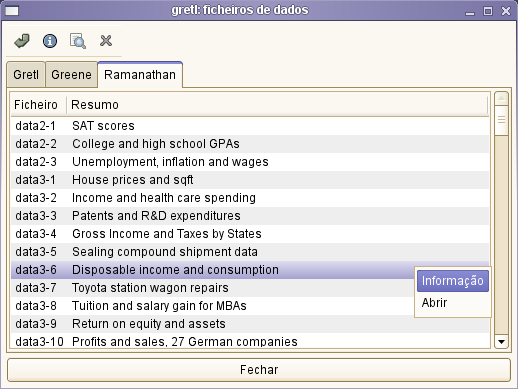
\includegraphics[scale=0.5]{figures/datafiles}
  \end{center}
\end{figure}

Selezionando una riga in questa finestra e facendo clic su ``Info'',
si aprir� una finestra di descrizione del dataset in questione (che
pu� contenere informazioni a proposito della fonte dei dati e della
definizione delle variabili).  Se si trova un file interessante, �
possibile aprirlo facendo clic su ``Apri'', o semplicemente facendo
doppio clic sul nome del file. Per il momento, apriamo \verb+data3-6+.
\tip{Nelle finestre di \app{gretl} che contengono liste, facendo
  doppio clic su una riga viene eseguita l'azione predefinita per la
  relativa voce nella lista: ad esempio mostrare i valori di una
  serie, o aprire un file.  } Questo file contiene dati relativi a un
oggetto classico dell'econometria, la funzione di consumo. La finestra
dei dati dovrebbe ora contenere il nome del file di dati in uso,
l'intervallo completo dei dati e quello del campione, i nomi delle
variabili, insieme a delle loro brevi descrizioni (si veda la Figure
\ref{fig-mainwin}).
    
\begin{figure}[htbp]
  \caption{Finestra principale, con un file di esempio aperto}
  \label{fig-mainwin}
  \begin{center}
    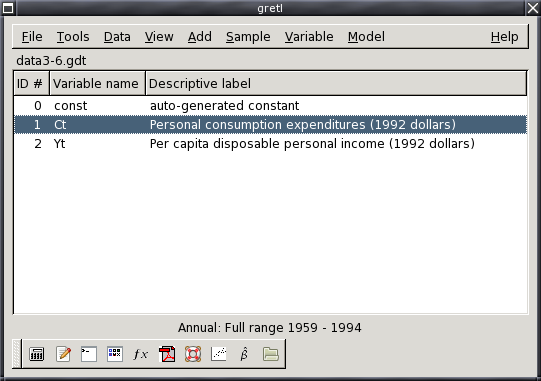
\includegraphics[scale=0.5]{figures/mainwin}
  \end{center}
\end{figure}

OK, cosa possiamo fare ora? Le varie opzioni dei men� dovrebbero
essere abbastanza chiare: per ora ci concentreremo sul men� Modello,
ma una panoramica di tutti i men� della finestra principale � fornita
pi� avanti (si veda Section \ref{menus}).
    
Il men� Modello di \app{gretl} offre varie routine di stima
econometrica: quella pi� semplice e nota � rappresentata dai minimi
quadrati ordinari (Ordinary Least Squares - OLS). Scegliendo OLS, si
apre una finestra di dialogo che richiede una \emph{specificazione del
  modello}; si veda la Figure \ref{fig-selector}.
    
\begin{figure}[htbp]
  \caption{Specificazione del modello}
  \label{fig-selector}
  \begin{center}
    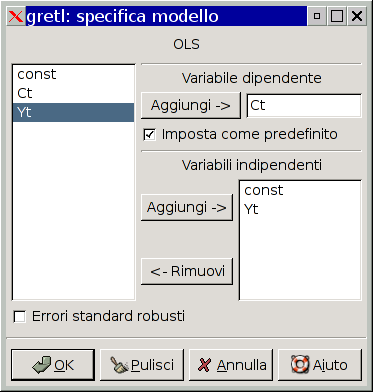
\includegraphics[scale=0.5]{figures/selector}
  \end{center}
\end{figure}
Per selezionare la variabile dipendente, fare clic su una variabile
nella lista di sinistra e premere il pulsante ``Scegli'' con la
freccia che punta verso il riquadro della variabile dipendente.
Selezionando la casella ``Imposta come predefinito'', la variabile
scelta verr� sempre pre-selezionata come variabile dipendente durante
le prossime aperture della finestra di dialogo.  Trucco: facendo
doppio clic su una variabile sulla sinistra, viene selezionata come
variabile dipendente e impostata come scelta predefinita.  Per
selezionare le variabili indipendenti, fare clic su di esse nella
lista di sinistra e premere il pulsante ``Aggiungi'' (o fare clic col
pulsante destro del mouse). � possibile selezionare pi� variabili
contigue trascinando il mouse; se le variabili da selezionare non sono
contigue, occorre fare clic tenendo prenuto il tasto \verb+Ctrl+.  Per
eseguire una regressione con il consumo come variabile dipendente e il
reddito come variabile indipendente, fare clic su \verb+Ct+ nel
riquadro della variabile dipendente e aggiungere \verb+Yt+ alla lista
delle variabili indipendenti.

\section{Risultati della stima}
\label{est-output}


Una volta specificato un modello, apparir� una finestra che mostra i
risultati della regressione, in un formato sufficientemente chiaro e
standard (Figure \ref{fig-modelwin}).
    
\begin{figure}[htbp]
  \caption{Finestra dei risultati del modello}
  \label{fig-modelwin}
  \begin{center}
    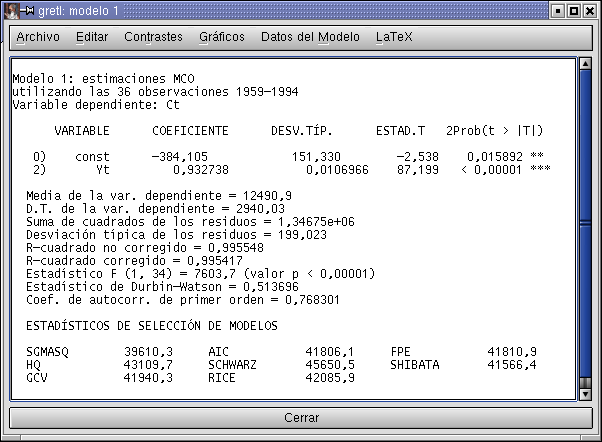
\includegraphics[scale=0.5]{figures/modelwin}
  \end{center}
\end{figure}
La finestra dei risultati contiene dei men� che consentono di
ispezionare o mostrare graficamente i residui e i valori stimati, e di
eseguire vari test diagnostici sul modello.Per la maggior parte dei
modelli c'� anche un'opzione per stampare il risultato della
regressione in formato {\LaTeX}. � possibile stampare i risultati in
formato tabulare (simile a quello usato nella finestra dei risultati,
ma con una migliore composizione tipografica) o sotto forma di
equazione. Per ognuna di queste opzioni � possibile scegliere di
vedere un'anteprima della pagina finale, o di salvare il risultato in
un file da includere in un documento {\LaTeX}. L'anteprima richiede
che si disponga di un sistema {\TeX} funzionante sul proprio computer.
� possibile controllare l'aspetto del {\LaTeX} generato da \app{gretl}
includendo un file chiamato \verb+gretlpre.tex+ nella propria
directory utente \app{gretl} (si veda XXX). Il contenuto di tale file
verr� usato come ``preambolo'' {\LaTeX}, il cui valore predefinito �
il seguente:
    
\begin{code}
      \documentclass[11pt]{article}
      \usepackage[latin1]{inputenc}
      \usepackage{amsmath}
      \usepackage{dcolumn,longtable}
      \begin{document}
      \thispagestyle{empty}
\end{code}

Si noti che sono richiesti i pacchetti \verb+amsmath+ e
\verb+dcolumn+.Per importare i risultati di \app{gretl}
in un word processor, � possibile fare copia e incolla da una
finestra dei risultati usando il men� \textsf{Modifica}
(o il pulsante Copia, in alcuni contesti) nel programma di arrivo.
Molte (non tutte) finestre di \app{gretl}
offrono l'opzione di copiare in formato RTF (il ``Rich Text
Format'' di Microsoft) o come {\LaTeX}. Se si deve incollare in
      un word processor, RTF pu� essere una buona opzione, visto che
      il formato tabulare dei risultati viene preservato\footnote{Si
noti 
che quando si copia come RTF in MS Windows,
          Windows permetter� di incollare il materiale solo in applicazioni
          che ``comprendono'' l'RTF. Quindi, sar� possibile
          incollare in MS Word, ma non nel Blocco Note. Inoltre sembra
          esserci un bug in alcune versioni di Windows, per cui
          l'operazione di copia non funziona se l'applicazione ``di
          arrivo'' (ad es. MS Word) non � stata avviata prima di
          copiare il materiale in questione.}.
      In alternativa, � possibile salvare i risultati come file di testo
      semplice e importare successivamente il file nel programma di arrivo:
      quando si conclude una sessione di \app{gretl}
      si ha l'opportunit� di salvare tutti i risultati della sessione in un
      unico file.Si noti che nel desktop \app{gnome} e in
      MS Windows, il men� \textsf{File} contiene un
      comando per inviare i risultati direttamente a una stampante.

    \tip{Quando si incollano o si importano dei risultati di
	\app{gretl} sotto forma di testo semplice in
        un word processor, conviene selezionare un carattere a spaziatura
        fissa, in stile macchina da scrivere (ad es. il Courier), per
        preservare il formato tabulare dei risultati. Selezionare un
        carattere non troppo grande (Courier da 10 punti dovrebbe andare
        bene) eviter�  che le righe dei risultati vengano spezzate nei
        punti sbagliati.}

\section{I men� della finestra principale}
\label{menus}


      Sulla barra dei men� della finestra principale si trovano,
      nell'ordine da sinistra a destra, i men� File, Utilit�, Sessione,
      Dati, Campione, Variabile, Modello e Aiuto.
    \begin{center}
      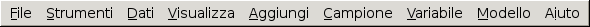
\includegraphics[scale=0.5]{figures/menubar}
    \end{center}

\begin{itemize}
\item \textsf{Men� file}
  \begin{itemize}
  \item \textsf{Apri dati}: apre un file di dati in formato interno di
    \app{gretl} o lo importa da altri formati. Si veda il [?].
  \item \textsf{Aggiungi dati}: Aggiunge dati al dataset in uso, da un
    file di dati di \app{gretl}, un file con dati separati da virgole,
    o un foglio elettronico.
  \item \textsf{Salva dati}: salva il file di dati \app{gretl} in uso.
              
  \item \textsf{Salva dati come}: salva il dataset in uso in formato
    interno, con la possibilit� di usare la compressione gzip. Si veda
    il [?].
	    
  \item \textsf{Esporta dati}: salva il dataset in uso in formato CSV
    (valori separati da virgole), o nei formati di GNU R o GNU Octave.
    Si veda il [?] e anche l'[?].
  \item \textsf{Abbandona dataset}: cancella dalla memoria il dataset
    in uso. Di solito questa operazione non � necessaria (visto che
    aprendo un nuovo file di dati, quello in uso viene sostituito), ma
    ci sono casi in cui � utile (si veda [?]).
  \item \textsf{Consulta database}: Si veda [?] e [?].
  \item \textsf{Crea dataset}: Apre il foglio elettronico integrato
    per inserire dati manualmente.  Si veda [?].
  \item \textsf{Visualizza log comandi}: Apre una finestra che
    contiene la registrazione dei comandi eseguiti finora.
  \item \textsf{Apri file comandi}: apre un file di comandi di
    \app{gretl} creato dall'utente o uno dei file di esempio forntiti
    con il programma. Se si intende creare un file di comandi da zero,
    occorre usare il comando successivo, \textsf{Nuovo file comandi}.
  \item \textsf{Preferenze}: imposta i percorsi per vari file a cui
    \app{gretl} deve accedere; sceglie i caratteri usati per mostrare
    i risultati; attiva la ``modalit� esperto'' (che sopprime la
    visualizzazione di alcuni messaggi di avvertimento); attiva o
    sopprime il controllo per la disponibilit� in rete di
    aggiornamenti di \app{gretl}; configura o disattiva la barra degli
    strumenti nella finestra principale.  Si veda il XXX per i
    dettagli.
  \item \textsf{Esci}: abbandona il programma.  Se non si � in
    modalit� esperto, verr� proposto di salvare il lavoro svolto.
  \end{itemize}


\item \textsf{Men� utilit�}
  \begin{itemize}
  \item \textsf{Tavole statistiche}: cerca i valori critici per alcune
    distribuzioni di uso comune (normale o Gaussiana, \emph{t},
    chi-quadro, \emph{F} e Durbin--Watson).
  \item \textsf{Calcola p-value}: apre una finestra che mostra i
    p-value per le distribuzioni Gaussiana, \emph{t}, chi-quadro,
    \emph{F} o gamma. Si veda anche il comando \cmd{pvalue} nel XXX.
  \item \textsf{Calcola test}: calcola le statistiche test e i p-value
    per una serie di test di ipotesi di uso comune (media della
    popolazione, varianza e proporzione, differenza delle medie o
    delle varianze e proporzioni). Occorre inserire nella finestra di
    dialogo le necessarie statistiche del campione. Alcuni semplici
    test richiedono che sia indicata una serie di dati, invece che
    delle statistiche del campione: si veda ``Differenza delle medie''
    e ``Differenza delle varianze'' nel men� Dati.
  \item \textsf{Terminale di Gretl}: apre una finestra di
    ``terminale'' in cui � possibile digitare dei comandi, come se si
    stesse usando la versione a riga di comando \app{gretlcli}, invece
    di quella con interfaccia grafica.
	    
  \item \textsf{Avvia Gnu R}: Avvia \app{R} (se � presente sul
    sistema) e vi carica una copia del dataset in uso in \app{gretl}.
    Si veda l'[?].
	    
  \item \textsf{Test NIST}: controlla l'accuratezza numerica di
    \app{gretl} usando i test di riferimento per la regressione
    lineare adottati dal National Institute of Standards and
    Technology statunitense.
  \end{itemize}


\item \textsf{Men� sessione}
  \begin{itemize}
  \item \textsf{Visualizza icone}: apre una finestra che mostra la
    sessione corrente di \app{gretl} sotto forma di un insieme di
    icone. Per i dettagli si veda [?].
	    
  \item \textsf{Apri}: apre un file di sessione salvato in precedenza.
	    
  \item \textsf{Salva}: salva la sessione corrente in un file.
	    
  \item \textsf{Salva come}: salva la sessione corrente in un file,
    scegliendone il nome.
	    
  \end{itemize}


\item \textsf{Men� Dati}
  \begin{itemize}
  \item \textsf{Mostra valori}: apre una finestra con un elenco (non
    modificabile) dei valori delle variabili (tutte o un sottoinsieme
    di esse).
  \item \textsf{Modifica valori}: apre una finestra di foglio
    elettronico, con cui � possibile modificare valori, aggiungere
    nuove variabili, o estendere il numero delle osservazioni.
	      
  \item \textsf{Ordina variabili}: riordina l'elenco delle variabili
    nella finestra principale, seguendo l'ordine numerico dell'ID o
    quello alfabetico del nome.
	      
  \item \textsf{Grafico delle variabili}: apre una finestra di dialogo
    che permette di scegliere tra un grafico temporale, un grafico a
    dispersione X--Y, un grafico X--Y a impulsi (barre verticali), un
    grafico X--Y ``con fattore'' (ossia, con i punti colorati in modo
    diverso a seconda del valore di una data variabile dummy), un
    boxplot e un grafico 3D.  Si veda il [?] per i dettagli.
  \item \textsf{Grafici multipli a dispersione}: mostra una raccolta
    di grafici (al massimo sei), con una variabile sull'asse \emph{y},
    rappresentata rispetto a diverse variabili sull'asse \emph{x},
    oppure con diverse variabili sull'asse \emph{y} rappresentate
    rispetto a una data variabile sull'asse \emph{x}. Pu� essere utile
    per l'analisi esplorativa dei dati.
  \item \textsf{Visualizza descrizione}, \textsf{Modifica
      descrizione}: ``Visualizza descrizione'' mostra le informazioni
    disponibili per il file di dati in uso; ``Modifica descrizione''
    permette di modificarle (se si ha il permesso di farlo).
  \item \textsf{Visualizza informazioni complete}: apre una finestra
    con una descrizione completa del dataset in uso, che include le
    informazioni di riepilogo e quelle specifiche di ogni variabile.
  \item \textsf{Statistiche descrittive}: mostra un insieme abbastanza
    ricco di statistiche descrittive per tutte le variabili del
    dataset, o per le variabili selezionate.
  \item \textsf{Matrice di correlazione}: mostra i coefficienti di
    correlazione per tutte le coppie di variabili nel dataset, o per
    quelle selezionate.
  \item \textsf{Componenti principali}: attivo solo se si selezionano
    due o pi� variabili; produce un'analisi delle componenti
    principali delle variabili selezionate.
          
  \item \textsf{Distanze di Mahalonobis}: attivo solo se si
    selezionano due o pi� variabili; calcola la distanza di
    Mahalonobis per ogni osservazione dal centroide dell'insieme di
    variabili selezionate.
          
  \item \textsf{Differenza delle medie}: calcola la statistica
    \emph{t} per l'ipotesi nulla che le medie della popolazione siano
    uguali per due variabili scelte, mostrando il p-value.
  \item \textsf{Differenza delle varianze}: calcola la statistica
    \emph{F} per l'ipotesi nulla che le varianze della popolazione
    siano uguali per due variabili scelte, mostrando il p-value.
  \item \textsf{Aggiungi variabili}: mostra un men� di trasformazioni
    standard per le variabili (logaritmi, ritardi, quadrati, ecc) che
    � possibile aggiungere al dataset. D� anche l'opzione di
    aggiungere variabili casuali e (per i dataset di serie storiche)
    variabili dummy stagionali (ad es. variabily dummy trimestrali per
    dati trimestrali). Include la possibilit� di impostare il seme del
    generatore di numeri pseudo-casuali.
  \item \textsf{Aggiorna finestra}: a volte i comandi di \app{gretl}
    generano nuove variabili. Questo comando sincronizza l'elenco
    delle variabili visualizzato nella finestra principale con
    l'elenco mantenuto internamente dal programma.
  \item \textsf{Aggiungi osservazioni}: Mostra una finestra di dialogo
    in cui � possibile scegliere un numero di osservazioni da
    aggiungere alla fine del dataset attuale; da usare per le
    previsioni.
           
  \item \textsf{Rimuove le osservazioni aggiuntive}: attivo solo se
    sono state aggiunte automaticamente delle osservazioni durante la
    procedura di previsione; cancella queste osservazioni aggiuntive.
           
  \end{itemize}


\item \textsf{Men� campione}
  \begin{itemize}
  \item \textsf{Imposta intervallo}: seleziona punti di partenza e
    arrivo diversi per il campione in uso, all'interno dell'intervallo
    di dati disponibili.
  \item \textsf{Ripristina campione completo}: si spiega da s�.
  \item \textsf{Struttura dataset}: permette di modificare
    l'interpretazione strutturale del dataset in uso. Ad esempio, se i
    dati sono stati importati come cross section, � possibile fare in
    modo che il programma li interpreti come serie storiche o come
    panel. Si veda anche il [?].
  \item \textsf{Compatta dati}: per serie storiche con frequenza
    superiore a quella annuale, permette di diminuire la frequenza dei
    dati, usando uno dei quattro metodi di compattamento disponibili
    (media, somma, inizio del periodo, fine del periodo).
  \item \textsf{Imposta in base a dummy}: data una variabile dummy
    (indicatore) con valori 0 o 1, vengono scartate dal campione tutte
    le osservazioni per cui la variabile dummy vale 0.
  \item \textsf{Imposta in base a condizione}: simile al precedente,
    tranne per il fatto che non si ha bisogno di una variabile
    predefinita: basta fornire una condizione Booleana (ad es.
    \verb+sqft > 1400+) e il campione sar� ristretto alle osservazioni
    che soddisfano la condizione. Si veda la voce \cmd{genr} nel XXX
    per maggiori dettagli sugli operatori Booleani che possono essere
    usati.
  \item \textsf{Scarta valori mancanti}: scarta dal campione corrente
    tutte le osservazioni per cui almeno una variabile ha un valore
    mancante (si veda [?]).
	    
  \item \textsf{Conta valori mancanti}: produce un rapporto sulle
    osservazioni per cui mancano dei valori. Pu� essere utile durante
    l'esame di un dataset panel, dove � abbastanza comune incontrare
    valori mancanti.
  \item \textsf{Imposta codice valori mancanti}: imposta il valore
    numerico che sar� interpretato come ``mancante'' o ``non
    disponibile''.
  \item \textsf{Aggiungi marcatori}: richiede di specificare un file
    di testo che contiene ``marcatori per le osservazioni'' (brevi
    stringhe che identificano singole osservazioni) e aggiunge queste
    informazioni al dataset. Si veda il [?].
  \item \textsf{Rimuovi marcatori}: attivo solo se il dataset contiene
    marcatori per le osservazioni; rimuove questi marcatori.
  \item \textsf{Ristruttura panel}: permette di convertire un dataset
    panel da una struttura "pila di dati cross-section" a una "pila di
    serie storiche", o viceversa. A differenza del comando
    \textsf{Struttura dataset}, questo modifica effettivamente
    l'organizzazione dei dati.
	    
  \item \textsf{Trasponi dati}: trasforma ogni osservazione in una
    variabile e viceversa (o, in altre parole, ogni riga della matrice
    dei dati diventa una colonna della nuova matrice dei dati); pu�
    essere utile per ``raddrizzare'' dati importati in modo errato.
           
  \end{itemize}


\item \textsf{Men� variabile}: la maggior parte di questi comandi
  operano su una sola variabile alla volta. La variabile ``attiva''
  viene impostata facendo clic sulla riga che la contiene nella
  finestra principale. La maggior parte delle opzioni si spiegano da
  sole.  Si noti che � possibile rinominare una variabile e modificare
  la sua etichetta descrittiva usando ``Modifica attributi''. � anche
  possibile definire una nuova variabile attraverso una formula (che
  pu� essere una funzione di una o pi� variabili esistenti). Per la
  sintassi di queste formule, si veda la sezione ``Definisci nuova
  variabile'' della guida in linea o la voce \cmd{genr}. Un semplice
  esempio:
	  
\begin{code}
	    pippo = x1 * x2
\end{code}

  creer� la nuova variabile \verb+pippo+ come prodotto delle variabili
  esistenti \verb+x1+ e \verb+x2+.  In queste formule, le variabili
  devono essere indicate per nome, non per numero identificativo.
\item \textsf{Men� modello}: per i dettagli sui vari stimatori offerti
  in questo men�, si consulti XXX oppure il capitolo ``Stima'' della
  guida in linea. Si veda anche il [?] a proposito della stima di
  modelli non lineari.
\item \textsf{Men� Aiuto}: usatelo!  Fornisce dettagli sulla sintassi
  dei comandi e delle finestre di dialogo.
\end{itemize}



\section{La barra degli strumenti di gretl}
\label{toolbar}

In basso a sinistra nella finestra principale si trova la barra
      degli strumenti.\begin{center}
        
\includegraphics[scale=0.5]{figures/toolbar}
      \end{center}
Le icone sulla barra hanno il seguente significato, nell'ordine:
\begin{enumerate}
\item Avvia una calcolatrice. Una funzione comoda quando si ha bisogno
  di usare velocemente una calcolatrice mentre si lavora in
  \app{gretl}. Il programma avviato in modo predefinito �
  \verb+calc.exe+ in MS Windows, o \verb+xcalc+ nel sistema X window.
  � possibile cambiare il programma nel men� \textsf{File, Preferenze,
    Generali}, sezione ``Programmi''.
          
\item Inizia un nuovo script. Apre una finestra in cui � possibile
  digitare una serie di comandi da eseguire in modalit� batch.
\item Apri il terminale di gretl. Una scorciatoia per il comando del
  men� ``Terminale di Gretl'' (si veda Section \ref{menus}).
\item Apri la finestra di sessione di gretl.
\item Apri il sito web di \app{gretl} nel proprio browser (funziona
  solo se si � connessi a internet e si dispone di un browser).
\item Apri l'ultima versione del manuale di gretl in formato PDF.
  Richiede una connessione a internet e un browser in grado di gestire
  i file PDF.
\item Apri la guida in linea per la sintassi dei comandi (che mostra i
  dettagli di tutti i comandi disponibili).
	  
\item Apri la finestra di dialogo per costruire un grafico.
	  
\item Apri la finestra di dialogo per stimare un modello con i minimi
  quadrati ordinari.
\item Apri una finestra che elenca i dataset relativi al libro
  \emph{Introductory Econometrics} di Ramanathan (e anche i dataset
  del libro di Jeffrey Wooldridge, se sono installati).
\end{enumerate}


      Se non si desidera visualizzare la barra degli strumenti, � possibile
      disabilitarla nel men� \textsf{File, Preferenze, Generali},
      de-selezionando la casella ``Mostra la barra degli strumenti di gretl''.

%%% Local Variables: 
%%% mode: latex
%%% TeX-master: "gretl-guide-it"
%%% End: 


\chapter{Modes of working}
\label{modes}

\section{Command scripts}
\label{scripts}

As you execute commands in \app{gretl}, using the GUI and filling in
dialog entries, those commands are recorded in the form of a
``script'' or batch file.  Such scripts can be edited and re-run,
using either \app{gretl} or the command-line client, \app{gretlcli}.

To view the current state of the script at any point in a \app{gretl}
session, choose ``Command log'' under the Tools menu. This log
file is called \verb+session.inp+ and it is overwritten whenever you
start a new session.  To preserve it, save the script under a
different name.  Script files will be found most easily, using the GUI
file selector, if you name them with the extension ``\verb+.inp+''.

To open a script you have written independently, use the ``File,
Script files'' menu item; to create a script from scratch use the
``File, Script files, New script'' item or the ``new script'' toolbar
button.  In either case a script window will open (see Figure
\ref{fig-scriptwin}).

\begin{figure}[htbp]
  \begin{center}
    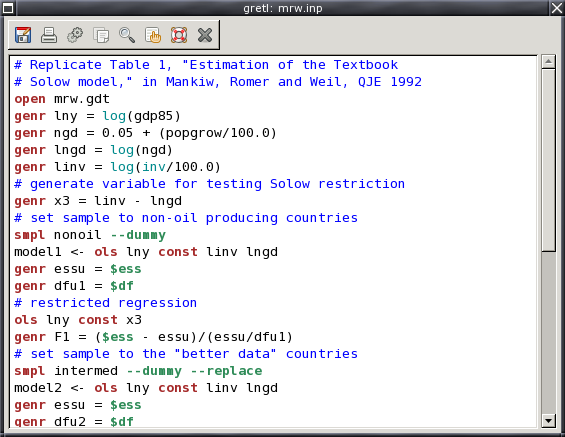
\includegraphics[scale=0.5]{figures/scriptwin}
  \end{center}
  \caption{Script window, editing a command file}
  \label{fig-scriptwin}
\end{figure}

The toolbar at the top of the script window offers the following
functions (left to right): (1) Save the file; (2) Save the file under
a specified name; (3) Print the file (this option is not available on
all platforms); (4) Execute the commands in the file; (5) Copy
selected text; (6) Paste the selected text; (7) Find and replace text;
(8) Undo the last Paste or Replace action; (9) Help (if you place the
cursor in a command word and press the question mark you will get help
on that command); (10) Close the window.

When you execute the script, by clicking on the Execute icon or by
pressing Ctrl-r, all output is directed to a single window, where it
can be edited, saved or copied to the clipboard.  To learn more about
the possibilities of scripting, take a look at the \app{gretl} Help
item ``Command reference,'' or start up the command-line program
\app{gretlcli} and consult its help, or consult the \GCR.

If you run the script when part of it is highlighted, \app{gretl} will
only run that portion. Moreover, if you want to run just the current
line, you can do so by pressing Ctrl-Enter.\footnote{This feature is
  not unique to \app{gretl}; other econometric packages offer the same
  facility. However, experience shows that while this can be
  remarkably useful, it can also lead to writing dinosaur scripts that
  are never meant to be executed all at once, but rather used as a
  chaotic repository to cherry-pick snippets from. Since \app{gretl}
  allows you to have several script windows open at the same time, you
  may want to keep your scripts tidy and reasonably small.}

Clicking the right mouse button in the script editor window produces a
pop-up menu.  This gives you the option of executing either the line
on which the cursor is located, or the selected region of the script
if there's a selection in place.  If the script is editable, this menu
also gives the option of adding or removing comment markers from the
start of the line or lines.

The \app{gretl} package includes over 70 ``practice'' scripts.  Most
of these relate to \cite{ramanathan02}, but they may also be used as a
free-standing introduction to scripting in \app{gretl} and to various
points of econometric theory.  You can explore the practice files
under ``File, Script files, Practice file'' There you will find a
listing of the files along with a brief description of the points they
illustrate and the data they employ.  Open any file and run it to see
the output.  Note that long commands in a script can be broken over
two or more lines, using backslash as a continuation character.

You can, if you wish, use the GUI controls and the scripting approach
in tandem, exploiting each method where it offers greater convenience.
Here are two suggestions.

\begin{itemize}
\item Open a data file in the GUI.  Explore the data --- generate
  graphs, run regressions, perform tests.  Then open the Command log,
  edit out any redundant commands, and save it under a specific name.
  Run the script to generate a single file containing a concise record
  of your work.
\item Start by establishing a new script file.  Type in any commands
  that may be required to set up transformations of the data (see the
  \cmd{genr} command in the \GCR). Typically this sort of thing can be
  accomplished more efficiently via commands assembled with
  forethought rather than point-and-click. Then save and run the
  script: the GUI data window will be updated accordingly.  Now you
  can carry out further exploration of the data via the GUI.  To
  revisit the data at a later point, open and rerun the
  ``preparatory'' script first.
\end{itemize}

\subsection{Scripts and data files}

One common way of doing econometric research with \app{gretl} is as
follows: compose a script; execute the script; inspect the output;
modify the script; run it again --- with the last three steps repeated
as many times as necessary.  In this context, note that when you open
a data file this clears out most of \app{gretl}'s internal state.
It's therefore probably a good idea to have your script start with an
\texttt{open} command: the data file will be re-opened each time, and
you can be confident you're getting ``fresh'' results.

One further point should be noted.  When you go to open a new data
file via the graphical interface, you are always prompted: opening a
new data file will lose any unsaved work, do you really want to do
this?  When you execute a script that opens a data file, however, you
are \textit{not} prompted.  The assumption is that in this case you're
not going to lose any work, because the work is embodied in the script
itself (and it would be annoying to be prompted at each iteration of
the work cycle described above).   

This means you should be careful if you've done work using the
graphical interface and then decide to run a script: the current data
file will be replaced without any questions asked, and it's your
responsibility to save any changes to your data first.


\section{Saving script objects}
\label{sect-script-objects}

When you estimate a model using point-and-click, the model results are
displayed in a separate window, offering menus which let you perform
tests, draw graphs, save data from the model, and so on.  Ordinarily,
when you estimate a model using a script you just get a
non-interactive printout of the results.  You can, however, arrange
for models estimated in a script to be ``captured'', so that you can
examine them interactively when the script is finished.  Here is an
example of the syntax for achieving this effect:
    
\begin{code}
Model1 <- ols Ct 0 Yt
\end{code}
That is, you type a name for the model to be saved under, then a
back-pointing ``assignment arrow'', then the model command.  You may
use names that have embedded spaces if you like, but such names must
be wrapped in double quotes:
\begin{code}
"Model 1" <- ols Ct 0 Yt
\end{code}
Models saved in this way will appear as icons in the \app{gretl}
icon view window (see Section \ref{session}) after the script is
executed.  In addition, you can arrange to have a named model
displayed (in its own window) automatically as follows:
\begin{code}
Model1.show
\end{code}
Again, if the name contains spaces it must be quoted:
\begin{code}
"Model 1".show
\end{code}
The same facility can be used for graphs.  For example the following
will create a plot of \verb+Ct+ against \verb+Yt+, save it under the
name ``CrossPlot'' (it will appear under this name in the icon
view window), and have it displayed:
\begin{code}
CrossPlot <- gnuplot Ct Yt
CrossPlot.show
\end{code}
You can also save the output from selected commands as named pieces of
text (again, these will appear in the session icon window, from where
you can open them later).  For example this command sends the output
from an augmented Dickey--Fuller test to a ``text object'' named
\verb+ADF1+ and displays it in a window:
\begin{code}
ADF1 <- adf 2 x1
ADF1.show
\end{code}
Objects saved in this way (whether models, graphs or pieces of text
output) can be destroyed using the command \verb+.free+ appended to
the name of the object, as in \verb+ADF1.free+.

\section{The gretl console}
\label{console}

A further option is available for your computing convenience. Under
\app{gretl}'s ``Tools'' menu you will find the item ``Gretl console''
(there is also an ``open gretl console'' button on the toolbar in the
main window).  This opens up a window in which you can type commands
and execute them one by one (by pressing the Enter key) interactively.
This is essentially the same as \app{gretlcli}'s mode of operation,
except that the GUI is updated based on commands executed from the
console, enabling you to work back and forth as you wish.

In the console, you have ``command history''; that is, you can use the
up and down arrow keys to navigate the list of command you have
entered to date.  You can retrieve, edit and then re-enter a previous
command.

In console mode, you can create, display and free objects (models,
graphs or text) aa described above for script mode.

\section{The Session concept}
\label{session}

\app{gretl} offers the idea of a ``session'' as a way of keeping track
of your work and revisiting it later. The basic idea is to provide an
iconic space containing various objects pertaining to your current
working session (see Figure \ref{fig-session}).  You can add objects
(represented by icons) to this space as you go along.  If you save the
session, these added objects should be available again if you re-open
the session later.

\begin{figure}[htbp]
  \begin{center}
    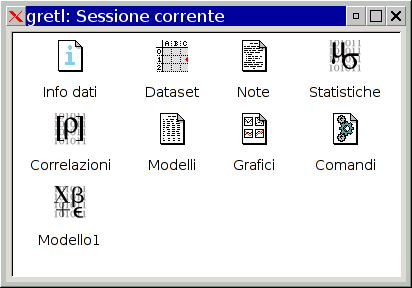
\includegraphics[scale=0.5]{figures/session}
  \end{center}
  \caption{Icon view: one model and one graph have been added to the
    default icons}
  \label{fig-session}
\end{figure}

If you start \app{gretl} and open a data set, then select ``Icon
view'' from the View menu, you should see the basic default set of
icons: these give you quick access to information on the data set (if
any), correlation matrix (``Correlations'') and descriptive summary
statistics (``Summary''). All of these are activated by
double-clicking the relevant icon.  The ``Data set'' icon is a little
more complex: double-clicking opens up the data in the built-in
spreadsheet, but you can also right-click on the icon for a menu of
other actions.

To add a model to the Icon view, first estimate it using the Model
menu.  Then pull down the File menu in the model window and select
``Save to session as icon\dots{}'' or ``Save as icon and close''.
Simply hitting the \verb+S+ key over the model window is a shortcut to
the latter action.

To add a graph, first create it (under the View menu, ``Graph
specified vars'', or via one of \app{gretl}'s other graph-generating
commands).  Click on the graph window to bring up the graph menu, and
select ``Save to session as icon''.

Once a model or graph is added its icon will appear in the Icon view
window.  Double-clicking on the icon redisplays the object, while
right-clicking brings up a menu which lets you display or delete the
object.  This popup menu also gives you the option of editing graphs.

\subsection{The model table}
\label{model-table}

In econometric research it is common to estimate several models with a
common dependent variable --- the models differing in respect of which
independent variables are included, or perhaps in respect of the
estimator used.  In this situation it is convenient to present the
regression results in the form of a table, where each column contains
the results (coefficient estimates and standard errors) for a given
model, and each row contains the estimates for a given variable across
the models.  

In the Icon view window \app{gretl} provides a means of constructing
such a table (and copying it in plain text, {\LaTeX} or Rich Text
Format).  The procedure is outlined below.  (The model table can also
be built non-interactively, in script mode.  For details, see the
entry for \cmd{modeltab} in the \emph{Gretl Command Reference}.)

      
\begin{enumerate}
\item Estimate a model which you wish to include in the table, and in
  the model display window, under the File menu, select ``Save to
  session as icon'' or ``Save as icon and close''.
\item Repeat step 1 for the other models to be included in the table
  (up to a total of six models).
\item When you are done estimating the models, open the icon view of
  your gretl session, by selecting ``Icon view'' under the View
  menu in the main gretl window, or by clicking the ``session icon
  view'' icon on the gretl toolbar.
\item In the Icon view, there is an icon labeled ``Model table''.
  Decide which model you wish to appear in the left-most column of the
  model table and add it to the table, either by dragging its icon
  onto the Model table icon, or by right-clicking on the model icon
  and selecting ``Add to model table'' from the pop-up menu.
\item Repeat step 4 for the other models you wish to include in the
  table.  The second model selected will appear in the second column
  from the left, and so on.
\item When you are finished composing the model table, display it by
  double-clicking on its icon.  Under the Edit menu in the window
  which appears, you have the option of copying the table to the
  clipboard in various formats.
\item If the ordering of the models in the table is not what you
  wanted, right-click on the model table icon and select ``Clear
  table''.  Then go back to step 4 above and try again.
\end{enumerate}

A simple instance of \app{gretl}'s model table is shown in
Figure~\ref{fig-model-table}.

\begin{figure}[htbp]
  \begin{center}
    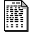
\includegraphics[scale=0.5]{figures/model_table}
  \end{center}
  \caption{Example of model table}
  \label{fig-model-table}
\end{figure}


\subsection{The graph page}
\label{sect-graphpage}

The ``graph page'' icon in the session window offers a means of
putting together several graphs for printing on a single page.  This
facility will work only if you have the {\LaTeX} typesetting system
installed, and are able to generate and view either PDF or PostScript
output.  The output format is controlled by your choice of program for
compiling \TeX\ files, which can be found under the ``Programs'' tab
in the Preferences dialog box (under the ``Tools'' menu in the main
window).  Usually this should be \app{pdflatex} for PDF output or
\app{latex} for PostScript.  In the latter case you must have
a working set-up for handling PostScript, which will
usually include \app{dvips}, \app{ghostscript} and a viewer such
as \app{gv}, \app{ggv} or \app{kghostview}.  

In the Icon view window, you can drag up to eight graphs onto the
graph page icon.  When you double-click on the icon (or right-click
and select ``Display''), a page containing the selected graphs (in PDF
or EPS format) will be composed and opened in your viewer.  From there
you should be able to print the page.

To clear the graph page, right-click on its icon and select ``Clear''.

As with the model table, it is also possible to manipulate the graph
page via commands in script or console mode --- see the entry for the
\cmd{graphpg} command in the \emph{Gretl Command Reference}.


\subsection{Saving and re-opening sessions}
\label{session-save}

If you create models or graphs that you think you may wish to
re-examine later, then before quitting \app{gretl} select ``Session
files, Save session'' from the File menu and give a name under
which to save the session.  To re-open the session later, either

\begin{itemize}
\item Start \app{gretl} then re-open the session file by going to the
  ``File, Session files, Open session'', or
\item From the command line, type \cmd{gretl -r} \textsl{sessionfile},
  where \textsl{sessionfile} is the name under which the session was
  saved, or
\item Drag the icon representing a \app{gretl} session file onto
  \app{gretl}.
\end{itemize}


%%% Local Variables: 
%%% mode: latex
%%% TeX-master: "gretl-guide"
%%% End: 


\chapter{File di dati}
\label{datafiles}



\section{Formato interno}
\label{native-format}

\app{gretl} ha un formato nativo per i file di dati. La maggior parte
degli utenti probabilmente non � interessata a leggere o scrivere
questi file con altri programmi che non siano \app{gretl}, ma in
alcune occasioni potrebbe essere utile farlo: per ulteriori dettagli
si veda l'[?].

\section{Altri formati dei file di dati}
\label{other-formats}


\app{gretl} legge anche file in altri formati:
    
\begin{itemize}
\item File di testo semplice (ASCII). Possono essere importati in
  \app{gretl} usando il comando ``File, Apri dati, Importa
  ASCII\dots{}'' dell'interfaccia grafica o il comando \cmd{import}
  dell'interfaccia a riga di comando. Per ulteriori dettagli su questo
  tipo di file, si veda Section \ref{scratch}.
\item File con valori separati da virgole (CSV).  Possono essere
  importati in \app{gretl} usando il comando ``File, Apri dati,
  Importa CSV\dots{}'' dell'interfaccia grafica o il comando
  \cmd{import} dell'interfaccia a riga di comando.  Si veda anche
  Section \ref{scratch}.
\item Cartelle di lavoro in formato \app{MS Excel} o \app{Gnumeric}.
  Possono essere importate in \app{gretl} con il comando ``File, Apri
  dati, Importa''.  Section \ref{scratch} descrive i requisiti per
  questo tipo di file.
\item Dati in formato BOX1. Il
  \href{http://www.census.gov/ftp/pub/DES/www/welcome.html}{Data
    Extraction Service} del Bureau of the Census statunitense offre
  (gratuitamente) molti dati microeconomici in questo formato.  I dati
  BOX1 possono essere importati con il comando ``File, Apri dati,
  Importa BOX\dots{}'', oppure con il comando \cmd{import -o}.
\end{itemize}

Quando vengono importati file in formato ASCII, CSV o BOX, \app{gretl}
apre una finestra ``diagnostica'', che informa sullo stato della
lettura dei dati. Se dovessero verificarsi dei problemi a causa di
dati malformattati, questa finestra mostrer� dei suggerimenti per
risolverli.Per venire incontro a chi vuole eseguire analisi pi�
sofisticate, \app{gretl} offre la possibilit� di salvare i dati nei
formati usati dai programmi GNU R e GNU Octave (si veda l'[?]).
Nell'interfaccia grafica, questa opzione si trova nel men� ``File'',
mentre nel client a riga di comando occorre usare il comando
\cmd{store} con l'opzione \cmd{-r} (per R) o \cmd{-m} (per Octave).

\section{Database binari}
\label{dbase}

Per lavorare con grandi quantit� di dati, \app{gretl} include una
routine per operare su database binari. Un \emph{database}, al
contrario di un \emph{file di dati}, non viene letto direttamente
nello spazio di lavoro del programma, ma pu� contenere serie con
frequenze e intervalli del campione diversi.  � possibile aprire un
database, selezionare delle serie e importarle nel dataset corrente;
le serie potranno poi essere salvate in un file di dati. � possibile
accedere ai database attraverso il comando ``File, Consulta
database''.Per i dettagli sul formato dei database di \app{gretl}, si
veda l'[?].

\subsection{Accesso ai database online}
\label{online-data}

Dalla versione 0.40, \app{gretl} � in grado di accedere ai database
via internet. Alla Wake Forest University sono disponibili alcuni
database, a cui � possibile accedere se il proprio computer � connesso
a internet. Si veda la voce ``Accesso ai database online'' nel men�
Aiuto di \app{gretl}.

\subsection{Database RATS 4}
\label{RATS}

Grazie a Thomas Doan di \emph{Estima}, che mi ha fornito le specifiche
del formato di database usato da RATS 4 (Regression Analysis of Time
Series), \app{gretl} � in grado di gestire anche alcuni tipi di
database RATS 4: per la precisione quelli che contengono dati mensili
o trimestrali.  La mia universit� possiede il database RATS G7, che
contiene dati per i sette maggiori paesi dell'OECD, e \app{gretl} lo
legge correttamente.\tip{Per dettagli e aggiornamenti sui dati
  disponibili, � possibile visitare la
  \href{http://gretl.sourceforge.net/gretl_data_it.html}{pagina dei
    dati} di \app{gretl}.}

\section{Creare un file di dati da zero}
\label{scratch}

Ci sono cinque modi per compiere questa operazione.
\begin{enumerate}
\item Acquisire, o creare con un editor di testo, un file di testo
  semplice ed aprirlo con il comando ``Importa ASCII'' di \app{gretl}.
       
\item Usare il proprio foglio di lavoro per inserire i dati, salvarlo
  in formato con valori separati da virgole (Comma Separated Values)
  se necessario (non dovrebbe essere necessario se il programma di
  foglio elettronico � MS Excel o Gnumeric) e infine usare uno dei
  comandi ``Importa'' di \app{gretl} (CSV, Excel o Gnumeric).
       
\item Usare il foglio elettronico contenuto in \app{gretl}.
       
\item Selezionare le serie di dati da un database.
       
\item Usare un editor di testo o altri programmi per creare un file di
  dati nel formato interno di \app{gretl}.
       
\end{enumerate}

Seguono alcune note a proposito dei vari metodi presentati.

\subsection{Note comuni sui dati importati}


Le opzioni 1 e 2 richiedono di usare il comando ``import'' di
\app{gretl}.  Affinch� i dati vengano letti correttamente, occorre che
siano soddisfatte alcune condizioni:
\begin{itemize}
\item La prima riga deve contenere nomi di variabile validi, ossia
  lunghi al massimo 8 caratteri (i nomi di variabile pi� lunghi
  verranno troncati a 8 caratteri), che iniziano con una lettera e
  sono composti solo da caratteri alfanumerici e dal carattere
  trattino basso, \verb+_+.  Precisazioni per i file ASCII o CSV: se
  il file non contiene righe con i nomi delle variabili, il programma
  user� automaticamente i nomi \verb+v1+, \verb+v2+ e cos� via.
  Inoltre, per ``prima riga'' si intende la prima riga
  \emph{significativa}: nel caso dei file ASCII e CSV, le righe
  bianche e quelle che iniziano con un carattere cancelletto,
  \verb+#+, vengono ignorate. Nel caso dell'importazione di file Excel
  e Gnumeric, viene presentata una finestra di dialogo in cui �
  possibile indicare il numero di righe e/o di colonne del foglio di
  lavoro da ignorare.
	  
\item I valori dei dati devono costituire un blocco rettangolare, con
  una variabile per colonna e un'osservazione per riga.  Il numero
  delle varibili (colonne dei dati) deve corrispondere al numero dei
  nomi di variabile specificati.  Si veda anche Section
  \ref{missing-data}. Il programma si aspetta dati di tipo numerico,
  ma nel caso di importazione da file ASCII/CSV, c'� un supporto
  limitato per dati di tipo carattere (stringa): se una colonna
  contiene solo dati di tipo stringa, le stringhe sono sostituite da
  codici numerici progressivi, e quando l'importazione si conclude,
  viene mostrata una tabella di corrispondenza tra stringhe e codici.
	  
\item Date (o marcatori per le osservazioni): opzionalmente, la
  \emph{prima} colonna pu� contenere stringhe, come date o etichette
  identificative per osservazioni su dati cross-section. Queste
  stringhe possono essere lunghe al massimo 8 caratteri (come avviene
  per le variabili, i nomi pi� lunghi verranno troncati), mentre la
  colonna che le ospita dovrebbe avere come nome \verb+obs+ o
  \verb+date+, oppure nessun nome.Affinch� una stringa sia
  riconosciuta come data, deve rispettare uno dei formati seguenti:
  per le serie \emph{annuali}, l'anno deve essere indicato con quattro
  cifre; per le serie \emph{trimestrali} occorre indicare l'anno con
  quattro cifre, seguito da un separatore (punto, due punti, o la
  lettera \verb+Q+) e da una cifra che indica il trimestre, ad
  esempio: \verb+1997.1+, \verb+2002:3+, \verb+1947Q1+; per le serie
  \emph{mensili} occorre indicare l'anno con quattro cifre, seguito
  dal punto o dai due punti, e da due cifre che indicano il mese, ad
  esempio: \verb+1997.01+, \verb+2002:10+.
	  
\end{itemize}

I file CSV possono usare virgole, spazi o tab come separatori fra le
colonne: il separatore da usare pu� essere selezionato subito dopo
aver eseguito il comando ``Importa CSV''. Se invece si usa ``Importa
ASCII'' il programma cerca di riconoscere automaticamente il
separatore usato nei dati.Se si usa un foglio elettronico per
preparare i dati, � possibile applicare varie trasformazioni ai dati
``grezzi'' (sommare variabili, calcolare percentuali, ecc.), ma queste
elaborazioni possono essere compiute, forse pi� facilmente, anche in
\app{gretl}, usando gli strumenti disponibili nel men� ``Dati,
Aggiungi variabili'' e/o ``Variabile, Definisci nuova variabile''.

\subsection{Importare dati e aggiungerli}


Pu� essere necessario costruire un dataset di \app{gretl} a poco a
poco, importando successivamente i dati da varie fonti. Questa
funzionalit� � fornita dai comandi del menu ``File, Aggiungi dati''.
\app{gretl} controller� che i nuovi dati siano compatibili con il
dataset esistente e in caso positivo aggiunger� i nuovi dati. In
questo modo � possibile aggiungere nuove variabili, a patto che la
frequenza dei dati corrisponda a quella del dataset esistente. � anche
possibile aggiungere nuove osservazioni per le serie di dati presenti
nel dataset; in questo caso i nomi delle variabili devono
corrispondere esattamente. Attenzione: se invece di ``Aggiungi dati''
si sceglie ``Apri dati'', il dataset corrente verr� chiuso.
	

\subsection{Usare il foglio elettronico interno}


� possibile creare un dataset con il comando ``File, Crea dataset'',
scegliendo il tipo di dati (ad es. serie storiche trimestrali, dati
cross-section), le date (o numero di osservazioni) iniziale e finale e
il nome della prima variabile da creare nel dataset. Dopo aver
effettuato queste scelte, viene presentato un semplice foglio
elettronico in cui � possibile iniziare a inserire i valori. Facendo
clic col tasto destro nella finestra del foglio elettronico, comparir�
un men� che permette di aggiungere una nuova variabile (colonna), di
aggiungere una nuova osservazione (aggiungere una riga in fondo al
foglio), o di inserire un'osservazione nel punto indicato (i dati
sottostanti saranno spostati in basso e verr� inserita una riga
vuota).Dopo aver inserito i dati nel foglio elettronico, � possibile
importarli nel foglio di lavoro di \app{gretl} premendo il pulsante
``Applica le modifiche'' nella finestra del foglio elettronico.Si noti
che il foglio elettronico di \app{gretl} � molto semplice e non
permette di inserire funzioni o formule: per trasformare i dati �
possibile usare i comandi disponibili nei men� ``Dati'' o
``Variabile'' nella finestra principale di \app{gretl}.

\subsection{Estrarre dati da un database}


Un modo alternativo di creare un dataset consiste nel selezionare le
variabili da un database.  \app{gretl} include un database di serie
storiche macroeconomiche relative agli USA e, come visto sopra,
consente di leggere i database RATS 4.Selezionando il comando ``File,
Consulta database'', vengono presentate tre alternative: ``gretl'',
``RATS 4'' e ``sul server di database''. Selezionando ``gretl'', si
trover� il file \verb+fedstl.bin+, che contiene un'ampia raccolta di
serie macroeconomiche USA ed � distribuito insieme al programma.Non si
trover� nulla sotto ``RATS 4'' a meno di non aver acquistato dei dati
RATS\footnote{Si veda \href{http://www.estima.com/}{www.estima.com}}.
Se si possiedono dati RATS, occorre usare il comando ``File,
Preferenze, Generali...'', selezionare la finestra Database e inserire
il percorso completo dei propri file RATS.Se il proprio computer �
connesso a internet � possibile accedere a vari database (alla Wake
Forest University) scegliendo ``sul server di database''. � possibile
consultare questi database da remoto, oppure installarli sul proprio
computer. La finestra dei database ha una colonna che mostra, per ogni
file, lo stato di installazione e lo stato di aggiornamento della
copia locale rispetto alla versione disponibile alla Wake Forest.Dopo
aver aperto un database � anche possibile importare singole serie
nello spazio di lavoro di \app{gretl} usando il comando ``Importa''
nella finestra del database, o nel men� che compare facendo clic col
tasto destro, oppure trascinando la serie nella finestra principale
del programma.
	

\subsection{Creare un file di dati nei formati interni di gretl}


Se si hanno gi� molti dati archiviati in formato elettronico,
l'approccio migliore pu� essere quello di creare un file di dati in
uno dei formati interni di \app{gretl}, usando un editor di testo o
altri programmi come \app{awk}, \app{sed} o \app{perl}. Ovviamente
occorrer� studiare i formati di dati di \app{gretl} (il formato XML o
quello ``tradizionale'') descritti nel chapter \ref{datafiles}.

\subsection{Nota aggiuntiva}



\app{gretl} non ha problemi a compattare serie di dati ad alta
frequenza (ad es. mensile) trasformandole in una frequenza pi� bassa
(ad es. trimestrale) utilizzando uno dei 4 metodi supportati (media
dei dati nel periodo, somma dei dati nel periodo, dato di inizio
periodo, dato di fine periodo).  Tuttavia, non c'� modo di convertire
dati a bassa frequenza in alta frequenza, quindi se si intende
importare serie con frequenza diversa da un database \emph{occorre
  iniziare ad importare le serie con la frequenza minore}. In questo
modo, il dataset di \app{gretl} verr� inizializzato con la frequenza
pi� bassa e i dati a frequenza maggiore potranno essere importati in
seguito (verranno compattati automaticamente). Se invece si inizia ad
importare dati ad alta frequenza, non sar� possibile importare serie a
frequenza pi� bassa in seguito.

\section{Valori mancanti nei dati}
\label{missing-data}

I valori mancanti vengono rappresentati internamente come
\verb+DBL_MAX+, il pi� alto numero in virgola mobile rappresentabile
sul sistema (che � probabile sia almeno 10 alla trecentesima potenza,
e non va interpretato come un valore legittimo dei dati).  Nei file di
dati in formato interno vanno rappresentati come \verb+NA+, mentre se
si importano dati in formato CSV \app{gretl} riconosce alcuni modi
comuni di rappresentare i valori mancanti: $-$999, la stringa
\verb+NA+ (in maiuscolo o minuscolo), un singolo punto, o
semplicemente una stringa vuota. Queste ultime, ovviamente, vanno
delimitate in modo opportuno, ad es. \verb+120.6,,5.38+ indica che il
valore di mezzo � mancante.Per quanto riguarda il trattamento dei
valori mancanti durante le analisi statistiche, \app{gretl} si
comporta nel modo seguente:
\begin{itemize}
\item Nel calcolo delle statistiche descrittive (media, deviazione
  standard, ecc.) con il comando \cmd{summary}, i valori mancanti sono
  semplicemente ignorati, e la dimensione del campione viene corretta
  adeguatamente.
\item Nel calcolo delle regressioni, \app{gretl} per prima cosa
  corregge l'inizio e la fine del campione, troncandolo dove occorre.
  Ad esempio, possono esserci dei valori mancanti all'inizio del
  campione perch� la regressione comprende serie differenziate,
  ritardate e cos� via. Oppure i valori mancanti possono trovarsi alla
  fine del campione, a causa della compresenza di serie con diverso
  livello di aggiornamento, o di serie anticipate.
\end{itemize}

Se \app{gretl} trova dei valori mancanti ``all'interno''
dell'intervallo del campione per una regressione (che pu� anche essere
troncato), il risultato dipende dal tipo di dataset e dallo stimatore
scelto. In molti casi, il programma eseguir� le stime saltando
automaticamente le osservazioni che contengono valori mancanti,
emettendo un messaggio che indica quante osservazioni sono state
escluse. Tuttavia, ci sono procedure che non saltano automaticamente
le osservazioni mancanti: tutti gli stimatori autoregressivi, gli
stimatori di sistema (come il SUR) e i minimi quadrati non lineari.
Nel caso di dati panel, l'esclusione automatica delle osservazioni
mancanti avviene solo se il dataset risultante costituisce un panel
"bilanciato". In tutti i casi in cui l'esclusione automatica delle
osservazioni mancanti non � supportata, \app{gretl} emette un
messaggio di errore e non produce stime.  In tutti i casi problematici
dovuti a valori mancanti all'interno di un dataset, � possibile
ricorrere alla funzione \cmd{misszero} (da usare con cautela!) del
comando \cmd{genr}. Eseguendo \cmd{genr pippo = misszero(pluto)} �
possibile produrre la serie \cmd{pippo}, che � identica a \cmd{pluto},
tranne per il fatto che tutti i valori mancanti sono stati trasformati
in zeri. In seguito, costruendo opportunamente delle variabili dummy,
sar� possibile eliminare dalla regressione le osservazioni che
contengono valori mancanti, pur mantenendo lo stesso intervallo del
campione\footnote{\cmd{genr} offre anche la funzione inversa di
  \cmd{misszero}, ossia \cmd{zeromiss}, che sostituisce in una serie i
  valori zero con il codice per i valori mancanti.}.
      

\section{Raccolte di file di dati}
\label{collections}


Se si usa \app{gretl} nell'attivit� didattica, pu� essere utile creare
una raccolta di file di dati e/o di script di comandi, personalizzati
per il proprio corso, ad uso degli studenti.A partire dalla versione
1.2.1 di \app{gretl}, ci sono tre modi per accedere a una raccolta di
file:
\begin{itemize}
\item Per i file di dati: selezionare dal men� ``File, Apri dati, File
  di esempio'', o fare clic sull'icona a forma di cartella sulla barra
  degli strumenti di \app{gretl}.
\item Per i file di comandi: selezionare dal men� ``File, Apri file
  comandi, File di esempio''.
\end{itemize}

Quando un utente seleziona uno dei comandi visti sopra:
\begin{itemize}
\item Vengono elencati automaticamente i file di dati o di comandi
  inclusi nella distribuzione di gretl (che comprendono i file
  relativi a \emph{Introductory Econometrics} di Ramanathan e a
  \emph{Econometric Analysis} di Greene).
\item Il programma cerca alcune raccolte di dati opzionali, ad esempio
  i file relativi ad alcuni libri di testo (Wooldridge, Gujarati,
  Stock e Watson) e la Penn World Table (PWT 5.6). Si veda
  \href{http://gretl.sourceforge.net/gretl_data_it.html}{la pagina dei
    dati} sul sito web di gretl per ulteriori informazioni su queste
  raccolte. Se queste raccolte vengono trovate, vengono aggiunte
  all'elenco dei file disponibili.
\item Il programma infine cerca delle raccolte di dati (non
  necessariamente note) nei posti seguenti: la directory ``di
  sistema'' dei file di dati, la directory di sistema dei file di
  comandi, la directory utente e tutte le loro sotto-directory di
  primo livello. Valori tipici per i nomi di queste directory sono
  mostrati nella Table \ref{tab-colls}.)
\end{itemize}

\begin{table}[htbp]
  \begin{center}
    \caption{Posizioni tipiche delle raccolte di file}
    \label{tab-colls}
    \begin{tabular}{p{2in}ll}
      � & Linux & MS Windows\\
        Directory di sistema per i dati & 
        \verb+/usr/share/gretl/data+ & 
        \verb+c:\userdata\gretl\data+\\
        Directory di sistema per i comandi & 
        \verb+/usr/share/gretl/scripts+ & 
        \verb+c:\userdata\gretl\scripts+\\
        Directory utente & \verb+/home/nomeutente/gretl+ & 
        \verb+c:\userdata\gretl\user+\\
      \end{tabular}
    \end{center}
  \end{table}

  Le raccolte trovate verranno aggiunte all'elenco dei file
  disponibili. In che formato deve essere una raccolta per essere
  riconosciuta come tale? Una raccolta pu� essere costituita da un
  gruppo di file di dati di \app{gretl} in fromato XML (con
  l'estensione \verb+.gdt+) o da un gruppo di file di comandi (con
  l'estensione \verb+.inp+), in entrambi i casi accompagnati da un
  ``file principale'' o catalogo.  La distribuzione di \app{gretl}
  contiene vari esempi di file di catalogo, ad esempio il file
  \verb+descriptions+ nella sottodirectory \verb+misc+ della directory
  dati di \app{gretl} e il file \verb+ps_descriptions+ nella
  sottodirectory \verb+misc+ della directory dei comandi.  Se si
  intende aggiungere una propria raccolta, occorrer� creare dei file
  di catalogo, chiamati \verb+descriptions+ per i file di dati, e
  \verb+ps_descriptions+ per i file di comandi, nelle rispettive
  directory (ad es.  \verb+/usr/share/gretl/data/mydata+ o
  \verb+c:\userdata\gretl\data\mydata+).La sintassi dei file di
  catalogo (che sono file di testo) � semplice; ecco ad esempio le
  prime righe del catalogo della raccolta di file di dati ``misc''
  inclusa nella distribuzione di gretl:
\begin{verbatim}
      # Gretl: various illustrative datafiles
      "arma","artificial data for ARMA script example"
      "ects_nls","Nonlinear least squares example"
      "hamilton","Prices and exchange rate, U.S. and Italy"
\end{verbatim}


  La prima riga, che deve iniziare con un carattere cancelletto,
  contiene un nome breve, qui ``Gretl'', che comparir� come etichetta
  identificativa per questa raccolta nella finestra di selezione dei
  dati, seguito da una virgola e da una descrizione breve della
  raccolta (opzionale).Le righe seguenti contengono due elementi,
  separati da una virgola e racchiusi tra virgolette doppie. Il primo
  � il nome del file di dati (escludendo l'estensione \verb+.gdt+),
  mentre il secondo � una breve descrizione del contenuto del file di
  dati. Dovrebbe esserci una riga come questa per ogni file di dati
  della raccolta.I file di catalogo per le raccolte di file di comandi
  sono molto simili a quelli appena visti, tranne per il fatto che
  ogni riga del file contiene tre campi: il nome del file (senza
  l'estensione \verb+.inp+), una breve descrizione del significato
  econometrico della serie di comandi contenuti nel file e una breve
  descrizione dei dati usati. Ecco un altro esempio: le prime righe
  del catalogo della raccolta di file di comandi ``misc'' inclusa
  nella distribuzione di gretl:
\begin{verbatim}
      # Gretl: various sample scripts
      "arma.inp","ARMA modeling","artificial data"
      "ects_nls","Nonlinear least squares (Davidson)","artificial data"
      "leverage","Influential observations","artificial data"
      "longley","Multicollinearity","US employment"
\end{verbatim}

  La procedura per creare la propria raccolta di dati e renderla
  disponibile agli utenti � la seguente:
  \begin{enumerate}
  \item Assemblare i dati, nel formato pi� comodo.
  \item Convertire i dati in formato \app{gretl} e salvarli come file
    \verb+gdt+. Probabilmente il modo pi� semplice consiste
    nell'importare i dati nel programma come testo semplice, CSV o
    formato foglio elettronico (MS Excel o Gnumeric) e quindi
    salvarli. Pu� essere utile aggiungere delle descrizioni delle
    singole variabili (usando il comando ``Variabile, Modifica
    attributi'') e delle informazioni sulle fonti dei dati (usando il
    comando ``Dati, Modifica descrizione'').
  \item Scrivere un file di catalogo per la raccolta, usando un editor
    di testi.
  \item Copiare i file di dati e il file di catalogo in una
    sottodirectory della directory dei dati (o utente) di \app{gretl}.
  \item Se la raccolta deve essere distribuita ad altri utenti, creare
    un pacchetto contenente i file di dati e il catalogo, ad esempio
    sotto forma di file zip.
  \end{enumerate}

  Se la raccolta creata non contiene dati proprietari, � possibile
  inviarla al curatore di \app{gretl} in modo che venga resa
  disponibile a tutti gli utenti del programma come pacchetto dati
  opzionale.

%%% Local Variables: 
%%% mode: latex
%%% TeX-master: "gretl-guide-it"
%%% End: 


\chapter{Special functions in genr}
\label{chap-genr}

\section{Introduction}
\label{genr-intro}

The \verb+genr+ command provides a flexible means of defining new
variables.  It is documented in the \GCR.  This chapter offers a more
expansive discussion of some of the special functions available via
\verb+genr+ and some of the finer points of the command.
    

\section{Time-series filters}
\label{genr-filter}

One sort of specialized function in \verb+genr+ is the time-series
filter.  Two such filters are currently available, the
Hodrick--Prescott filter and the Baxter--King bandpass filter. These
are accessed using \verb+hpfilt()+ and \verb+bkfilt()+ respectively:
in each case the function takes one argument, the name of the variable
to be processed.
    

\subsection{The Hodrick--Prescott filter}
\label{hodrick-prescott}

A time series $y_t$ may be decomposed into a trend or growth
component $g_t$ and a cyclical component $c_t$.  
%
\[
y_t = g_t + c_t, \quad t = 1,2,\dots,T
\]
%
The Hodrick--Prescott filter effects such a decomposition by
minimizing the following:
%
\[
    \sum_{t = 1}^T {(y_t - g_t )^2 } + \lambda \sum_{t = 2}^{T -
      1} \left((g_{t+1} - g_t) - (g_t - g_{t - 1} )\right)^2 .
\]
%
The first term above is the sum of squared cyclical components $c_t =
y_t - g_t$. The second term is a multiple $\lambda$ of the sum of
squares of the trend component's second differences. This
second term penalizes variations in the growth rate of the trend
component: the larger the value of $\lambda$, the higher is the
penalty and hence the smoother the trend series.

Note that the \cmd{hpfilt} function in \app{gretl} produces the
cyclical component, $c_t$, of the original series.  If you want the
smoothed trend you can subtract the cycle from the original:

\begin{code}
genr ct = hpfilt(yt)
genr gt = yt - ct
\end{code}

Hodrick and Prescott (1997) suggest that a value of $\lambda = 1600$
is reasonable for quarterly data.  The default value in \app{gretl} is
100 times the square of the data frequency (which, of course, yields
1600 for quarterly data).  The value can be adjusted using the
\cmd{set} command, with a parameter of \cmd{hp\_lambda}.  For example,
\cmd{set hp\_lambda 1200}.


\subsection{The Baxter and King filter}
\label{baxter-king}

Consider the spectral representation of a time series $y_t$:
%       
\[ y_t = \int_{-\pi}^{\pi} e^{i\omega} \mathrm{d} Z(\omega) \]
%
To extract the component of $y_t$ that lies between the frequencies
$\underline{\omega}$ and $\overline{\omega}$ one could apply a
bandpass filter:
%       
\[ c^*_t = \int_{-\pi}^{\pi} F^*(\omega) e^{i\omega} \mathrm{d}
Z(\omega) \]
%
where $F^*(\omega) = 1$ for $\underline{\omega} < |\omega| <
\overline{\omega}$ and 0 elsewhere. This would imply, in the time
domain, applying to the series a filter with an infinite number of
coefficients, which is undesirable. The Baxter and King bandpass
filter applies to $y_t$ a finite polynomial in the lag
operator $A(L)$:
%       
\[ c_t = A(L) y_t \]
%
where $A$($L$) is defined as
%       
\[ A(L) = \sum_{i=-k}^{k} a_i L^i \]

The coefficients $a_i$ are chosen such that $F(\omega)
= A(e^{i\omega})A(e^{-i\omega})$ is the best approximation to
$F^*(\omega)$ for a given $k$. Clearly, the higher $k$ the better the
approximation is, but since $2k$ observations have to be discarded, a
compromise is usually sought. Moreover, the filter has also other
appealing theoretical properties, among which the property that $A(1)
= 0$, so a series with a single unit root is made stationary by
application of the filter.

In practice, the filter is normally used with monthly or quarterly
data to extract the ``business cycle'' component, namely the component
between 6 and 36 quarters. Usual choices for $k$ are 8 or 12 (maybe
higher for monthly series).  The default values for the frequency
bounds are 8 and 32, and the default value for the approximation
order, $k$, is 8. You can adjust these values using the \cmd{set}
command. The keyword for setting the frequency limits is
\verb+bkbp_limits+ and the keyword for $k$ is \verb+bkbp_k+.  Thus for
example if you were using monthly data and wanted to adjust the
frequency bounds to 18 and 96, and $k$ to 24, you could do

\begin{code}
    set bkbp_limits 18 96
    set bkbp_k 24
\end{code}

These values would then remain in force for calls to the \verb+bkfilt+
function until changed by a further use of \verb+set+.
      

\section{Resampling and bootstrapping}
\label{genr-resample}

Another specialized function is the resampling, with replacement, of a
series.  Given an original data series \varname{x}, the command
\begin{code}
    genr xr = resample(x)
\end{code}
creates a new series each of whose elements is drawn at random from
the elements of \varname{x}.  If the original series has 100
observations, each element of \varname{x} is selected with probability
$1/100$ at each drawing.  This the effect is to ``shuffle'' the
elements of \varname{x}, with the twist that each element of
\varname{x} may appear more than once, or not at all, in \varname{xr}.

The primary use of this function is in the construction of bootstrap
confidence intervals or p-values.  Here is a simple example.  Suppose
we estimate a simple regression of $y$ on $x$ via OLS and find that
the slope coefficient has a reported $t$-ratio of 2.5 with 40 degrees
of freedom.  The two-tailed p-value for the null hypothesis that the
slope parameter equals zero is then 0.0166, using the $t(40)$
distribution.  Depending on the context, however, we may doubt whether
the ratio of coefficient to standard error truly follows the $t(40)$
distribution.  In that case we could derive a bootstrap p-value as
shown in Example~\ref{resample-loop}.  

Under the null hypothesis that the slope with respect to $x$ is zero,
$y$ is simply equal to its mean plus an error term.  We simulate $y$
by resampling the residuals from the initial OLS and re-estimate the
model.  We repeat this procedure a large number of times, and record
the number of cases where the absolute value of the $t$-ratio is
greater than 2.5: the proportion of such cases is our bootstrap
p-value.  For a good discussion of simulation-based tests and
bootstrapping, see Davidson and MacKinnon (2004, chapter 4).

\begin{script}[htbp]
  \caption{Calculation of bootstrap p-value}
  \label{resample-loop}
\begin{code}
    ols y 0 x
    # save the residuals
    genr ui = $uhat
    scalar ybar = mean(y)
    # number of replications for bootstrap
    scalar replics = 10000
    scalar tcount = 0
    series ysim = 0
    loop replics --quiet
      # generate simulated y by resampling
      ysim = ybar + resample(ui)
      ols ysim 0 x
      scalar tsim = abs(coeff(x) / stderr(x))
      tcount += (tsim > 2.5)
    endloop      
    printf "proportion of cases with |t| > 2.5 = %g\n", \
       tcount / replics
\end{code}
\end{script}
    

\section{Handling missing values}
\label{genr-missing}

Four special functions are available for the handling of missing
values.  The boolean function \verb+missing()+ takes the name of a
variable as its single argument; it returns a series with value 1 for
each observation at which the given variable has a missing value, and
value 0 otherwise (that is, if the given variable has a valid value at
that observation).  The function \verb+ok()+ is complementary to
\verb+missing+; it is just a shorthand for \verb+!missing+ (where
\verb+!+ is the boolean NOT operator).  For example, one can count the
missing values for variable \verb+x+ using

\begin{code}
    genr nmiss_x = sum(missing(x))
\end{code}

The function \verb+zeromiss()+, which again takes a single series as
its argument, returns a series where all zero values are set to the
missing code.  This should be used with caution --- one does not want
to confuse missing values and zeros --- but it can be useful in some
contexts.  For example, one can determine the first valid observation
for a variable \verb+x+ using

\begin{code}
    genr time
    genr x0 = min(zeromiss(time * ok(x)))
\end{code}

The function \verb+misszero()+ does the opposite of \verb+zeromiss+,
that is, it converts all missing values to zero.  

It may be worth commenting on the propagation of missing values within
\verb+genr+ formulae.  The general rule is that in arithmetical
operations involving two variables, if either of the variables has a
missing value at observation $t$ then the resulting series will also
have a missing value at $t$.  The one exception to this rule is
multiplication by zero: zero times a missing value produces zero
(since this is mathematically valid regardless of the unknown value).
    

\section{Retrieving internal variables}
\label{genr-internal}

The \verb+genr+ command provides a means of retrieving various values
calculated by the program in the course of estimating models or
testing hypotheses.  The variables that can be retrieved in this way
are listed in the \GCR; here we say a bit more about the special
variables \verb+$test+ and \verb+$pvalue+.

These variables hold, respectively, the value of the last test
statistic calculated using an explicit testing command and the p-value
for that test statistic.  If no such test has been performed at the
time when these variables are referenced, they will produce the
missing value code.  The ``explicit testing commands'' that work in
this way are as follows: \cmd{add} (joint test for the significance of
variables added to a model); \cmd{adf} (Augmented Dickey--Fuller test,
see below); \cmd{arch} (test for ARCH); \cmd{chow} (Chow test for a
structural break); \cmd{coeffsum} (test for the sum of specified
coefficients); \cmd{cusum} (the Harvey--Collier $t$-statistic);
\cmd{kpss} (KPSS stationarity test, no p-value available);
\cmd{lmtest} (see below); \cmd{meantest} (test for difference of
means); \cmd{omit} (joint test for the significance of variables
omitted from a model); \cmd{reset} (Ramsey's RESET); \cmd{restrict}
(general linear restriction); \cmd{runs} (runs test for randomness);
\cmd{testuhat} (test for normality of residual); and \cmd{vartest}
(test for difference of variances). In most cases both a \verb+$test+
and a \verb+$pvalue+ are stored; the exception is the KPSS test, for
which a p-value is not currently available.
    
An important point to notice about this mechanism is that the internal
variables \verb+$test+ and \verb+$pvalue+ are over-written each time
one of the tests listed above is performed.  If you want to reference
these values, you must do so at the correct point in the sequence of
\app{gretl} commands.  

A related point is that some of the test commands generate, by
default, more than one test statistic and p-value; in these cases only
the last values are stored. To get proper control over the retrieval
of values via \verb+$test+ and \verb+$pvalue+ you should formulate the
test command in such a way that the result is unambiguous.  This
comment applies in particular to the \verb+adf+ and \verb+lmtest+
commands.

\begin{itemize}
\item By default, the \cmd{adf} command generates three variants of
  the Dickey--Fuller test: one based on a regression including a
  constant, one using a constant and linear trend, and one using a
  constant and a quadratic trend.  When you wish to reference
  \verb+$test+ or \verb+$pvalue+ in connection with this command, you
  can control the variant that is recorded by using one of the flags
  \verb+--nc+, \verb+--c+, \verb+--ct+ or \verb+--ctt+ with
  \verb+adf+.
\item By default, the \cmd{lmtest} command (which must follow an OLS
  regression) performs several diagnostic tests on the regression in
  question.  To control what is recorded in \verb+$test+ and
  \verb+$pvalue+ you should limit the test using one of the flags
  \verb+--logs+, \verb+--autocorr+, \verb+--squares+ or
  \verb+--white+.
\end{itemize}

As an aid in working with values retrieved using \verb+$test+ and
\verb+$pvalue+, the nature of the test to which these values relate is
written into the descriptive label for the generated variable.  You
can read the label for the variable using the \cmd{label} command
(with just one argument, the name of the variable), to check that you
have retrieved the right value.  The following interactive session
illustrates this point.

\begin{code}
    ? adf 4 x1 --c

    Augmented Dickey-Fuller tests, order 4, for x1
    sample size 59
    unit-root null hypothesis: a = 1

      test with constant
      model: (1 - L)y = b0 + (a-1)*y(-1) + ... + e
      estimated value of (a - 1): -0.216889
      test statistic: t = -1.83491
      asymptotic p-value 0.3638

    P-values based on MacKinnon (JAE, 1996)
    ? genr pv = $pvalue
    Generated scalar pv (ID 13) = 0.363844
    ? label pv    
      pv=Dickey-Fuller pvalue (scalar)
\end{code}



%%% Local Variables: 
%%% mode: latex
%%% TeX-master: "gretl-guide"
%%% End: 


\chapter{Creare dei sotto-campioni}
\label{sampling}

\section{Introduzione}
\label{sample-intro}

Questo capitolo affronta alcune questioni correlate alla creazione di
sotto-campioni in un dataset.

� possibile definire un sotto-campione per un dataset in due modi
diversi, che chiameremo rispettivamente ``impostazione'' del campione
e ``restrizione'' del campione.
    
\section{Impostazione del campione}
\label{sample-set}

Per ``impostazione'' del campione, si intende la definizione di un
campione ottenuta indicando il punto iniziale e/o quello finale
dell'intervallo attuale del campione. Questa modalit� � usata
tipicamente con serie storiche; ad esempio se si hanno dati
trimestrali per l'intervallo da 1960:1 a 2003:4 e si vuole stimare una
regressione usando solo i dati degli anni '70, un comando adeguato �

\begin{code}
    smpl 1970:1 1979:4
\end{code}
      
Oppure se si vuole riservare la parte finale delle osservazioni
disponibili per eseguire una previsione "fuori dal campione", si pu�
usare il comando

\begin{code}
    smpl ; 2000:4
\end{code}
      
dove il punto e virgola significa ``mantenere inalterata
l'osservazione iniziale'' (e potrebbe essere usato in modo analogo al
posto del secondo parametro, indicando di mantenere inalterata
l'osservazione finale). Per ``inalterata'' in questo caso si intende
inalterata relativamente all'ultima impostazione eseguita con
\verb+smpl+, o relativamente all'intero dataset, se non � ancora stato
definito alcun sotto-campione in precedenza.  Ad esempio, dopo

\begin{code}
    smpl 1970:1 2003:4
    smpl ; 2000:4
\end{code}
      
l'intervallo del campione sar� da 1970:1 a 2000:4.

� possibile anche impostare l'intervallo del campione in modo incrementale o
relativo: in questo caso occorre indicare per il punto iniziale e finale uno
spostamento relativo, sotto forma di numero preceduto dal segno pi� o dal segno
meno (o da un punto e virgola per indicare nessuna variazione). Ad esempio

\begin{code}
    smpl +1 ;
\end{code}
      
sposter� in avanti di un'osservazione l'inizio del campione,
mantenendo inalterata la fine del campione, mentre

\begin{code}
    smpl +2 -1
\end{code}

sposter� l'inizio del campione in avanti di due osservazioni e la fine
del campione indietro di una.

Una caratteristica importante dell'operazione di ``impostazione del campione''
descritta fin qui � che il sotto-campione creato risulta sempre composto da un
insieme di osservazioni contigue. La struttura del dataset rimane quindi
inalterata: se si lavora su una serie trimestrale, dopo aver impostato il
campione la serie rimarr� trimestrale.
    

\section{Restrizione del campione}
\label{sample-restrict}

Per ``restrizione'' del campione si intende la definizione di un
campione ottenuta selezionando le osservazioni in base a un criterio
Booleano (logico), o usando un generatore di numeri casuali. Questa
modalit� � usata tipicamente con dati di tipo cross-section o panel.

Si supponga di avere dei dati di tipo cross-section che descrivono il
genere, il reddito e altre caratteristiche di un gruppo di individui e
si vogliano analizzare solo le donne presenti nel campione. Se si
dispone di una variabile dummy \verb+genere+, che vale 1 per gli
uomini e 0 per le donne, si potrebbe ottenere questo risultato con

\begin{code}
    smpl genere=0 --restrict
\end{code}
    
Oppure si supponga di voler limitare il campione di lavoro ai soli
individui con un reddito superiore ai 50.000 euro. Si potrebbe usare
\begin{code}
    smpl reddito>50000 --restrict
\end{code}

Qui sorge un problema: eseguendo in sequenza i due comandi visti
sopra, cosa conterr� il sotto-campione? Tutti gli individui con
reddito superiore a 50.000 euro o solo le donne con reddito superiore
a 50.000 euro? La risposta corretta � la seconda: la seconda
restrizione si aggiunge alla prima, ossia la restrizione finale � il
prodotto logico della nuova restrizione e di tutte le restrizioni
precedenti.  Se si vuole applicare una nuova restrizione
indipendentemente da quelle applicate in precedenza, occorre prima
re-impostare il campione alla sua lunghezza originaria, usando
    
\begin{code}
    smpl --full
\end{code}
%
In alternativa, � possibile aggiungere l'opzione \verb+replace+ al
comando \verb+smpl+:
%
\begin{code}
    smpl income>50000 --restrict --replace
\end{code}

Questa opzione ha l'effetto di re-impostare automaticamente il
campione completo prima di applicare la nuova restrizione.

A differenza della semplice ``impostazione'' del campione, la
``restrizione'' del campione pu� produrre un insieme di osservazioni
non contigue nel dataset originale e pu� anche modificare la struttura
del dataset.

Questo fenomeno pu� essere osservato nel caso dei dati
panel: si supponga di avere un panel di cinque imprese (indicizzate
dalla variabile \verb+impresa+) osservate in ognuno degli anni
identificati dalla variabile \verb+anno+.  La restrizione
%
\begin{code}
    smpl anno=1995 --restrict
\end{code}
%
produce un dataset che non � pi� di tipo panel, ma cross-section per
l'anno 1995.  In modo simile
%      
\begin{code}
    smpl impresa=3 --restrict
\end{code}
%
produce un dataset di serie storiche per l'impresa numero 3.

Per questi motivi (possibile non-contiguit� nelle osservazioni,
possibile cambiamento nella struttura dei dati) gretl si comporta in
modo diverso a seconda che si operi una ``restrizione'' del campione o
una semplice ``impostazione'' di esso. Nel caso dell'impostazione, il
programma memorizza semplicemente le osservazioni iniziali e finali e
le usa come parametri per i vari comandi di stima dei modelli, di
calcolo delle statistiche ecc. Nel caso della restrizione, il
programma crea una copia ridotta del dataset e la tratta come un
semplice dataset di tipo cross-section non datato.\footnote{Con una
  eccezione: se si parte da un dataset panel bilanciato e la
  restrizione � tale da preservare la struttura di panel bilanciato
  (ad esempio perch� implica la cancellazione di tutte le osservazioni
  per una unit� cross-section), allora il dataset ridotto � ancora
  trattato come panel.}

Se si vuole re-imporre un'interpretazione di tipo ``serie storiche'' o
``panel'' al dataset ridotto, occorre usare il comando \cmd{setobs}, o
il comando dal men� ``Campione, Struttura dataset'', se appropriato).

Il fatto che una ``restrizione'' del campione comporti la creazione di
una copia ridotta del dataset originale pu� creare problemi quando il
dataset � molto grande (nell'ordine delle migliaia di osservazioni).
Se si usano simili dataset, la creazione della copia pu� causare
l'esaurimento della memoria del sistema durante il calcolo dei
risultati delle regressioni. � possibile aggirare il problema in
questo modo:

\begin{enumerate}
\item Aprire il dataset completo e imporre la restrizione sul
  campione.
\item Salvare una copia del dataset ridotto su disco.
\item Chiudere il dataset completo e aprire quello ridotto.
\item Procedere con l'analisi.
\end{enumerate}

\section{Campionamento casuale}
\label{sample-random}

Se si usano dataset molto grandi (o se si intende studiare le
propriet� di uno stimatore), pu� essere utile estrarre un campione
casuale dal dataset completo. � possibile farlo ad esempio con

\begin{code}
    smpl 100 --random
\end{code}

che seleziona 100 osservazioni.  Se occorre che il campione sia
riproducibile, occorre per prima cosa impostare il seme del generatore
di numeri casuali, usando il comando \cmd{set}. Questo tipo di
campionamento � un esempio di ``restrizione'' del campione: viene
infatti generata una copia ridotta del dataset.

\section{I comandi del men� Campione}
\label{sample-menu}

Gli esempi visti finora hanno mostrato il comando testuale \cmd{set},
ma � possibile creare un sotto-campione usando i comandi del men�
\textsf{Campione} nell'interfaccia grafica del programma.

I comandi del men� permettono di ottenere gli stessi risultati delle
varianti del comando testuale \verb+smpl+, con la seguente eccezione:
se si usa il comando ``Campione, Imposta in base a condizione...'' e
sul dataset � gi� stato impostato un sotto-campione, viene data la
possibilit� di preservare la restrizione gi� attiva o di sostituirla
(in modo analogo a quanto avviene invocando l'opzione \verb+replace+
descritta nella parte~\ref{sample-restrict}.
    
%%% Local Variables: 
%%% mode: latex
%%% TeX-master: "gretl-guide-it"
%%% End: 


\chapter{Graphs and plots}
\label{chap-graphs}

\section{Gnuplot graphs}
\label{gnuplot-graphs}

A separate program, \app{gnuplot}, is called to generate graphs.
Gnuplot is a very full-featured graphing program with myriad options.
It is available from \href{http://www.gnuplot.info/}{www.gnuplot.info}
(but note that a suitable copy of gnuplot is bundled with the packaged
versions of gretl for MS Windows and Mac OS X).  Gretl gives you
direct access, via a graphical interface, to a subset of gnuplot's
options and it tries to choose sensible values for you; it also allows
you to take complete control over graph details if you wish.

With a graph displayed, you can click on the graph window for a pop-up
menu with the following options.

\begin{itemize}
\item \textsf{Save as PNG}: Save the graph in Portable Network
  Graphics format (the same format that you see on screen).
\item \textsf{Save as postscript}: Save in encapsulated postscript
  (EPS) format.
\item \textsf{Save as Windows metafile}: Save in Enhanced Metafile
  (EMF) format.
\item \textsf{Save to session as icon}: The graph will appear in
  iconic form when you select ``Icon view'' from the View menu.
\item \textsf{Zoom}: Lets you select an area within the graph for
  closer inspection (not available for all graphs).
\item \textsf{Print}: (Current GTK or MS Windows only) lets you
  print the graph directly.
\item \textsf{Copy to clipboard}: MS Windows only, lets you paste the
  graph into Windows applications such as MS Word.
\item \textsf{Edit}: Opens a controller for the plot which lets you
  adjust many aspects of its appearance.
\item \textsf{Close}: Closes the graph window.
\end{itemize}


\subsection{Displaying data labels}
\label{plot-labels}

For simple X-Y scatter plots, some further options are available if
the dataset includes ``case markers'' (that is, labels identifying
each observation).\footnote{For an example of such a dataset, see the
  Ramanathan file \verb+data4-10+: this contains data on private
  school enrollment for the 50 states of the USA plus Washington, DC;
  the case markers are the two-letter codes for the states.} With a
scatter plot displayed, when you move the mouse pointer over a data
point its label is shown on the graph.  By default these labels are
transient: they do not appear in the printed or copied version of the
graph.  They can be removed by selecting ``Clear data labels'' from
the graph pop-up menu. If you want the labels to be affixed
permanently (so they will show up when the graph is printed or
copied), select the option ``Freeze data labels'' from the pop-up
menu; ``Clear data labels'' cancels this operation.  The other
label-related option, ``All data labels'', requests that case markers
be shown for all observations.  At present the display of case markers
is disabled for graphs containing more than 250 data points.


\subsection{GUI plot editor}
\label{plot-editor}

Selecting the \textsf{Edit} option in the graph popup menu opens
an editing dialog box, shown in Figure~\ref{fig-plot}.  Notice that
there are several tabs, allowing you to adjust many aspects of
a graph's appearance: font, title, axis scaling, line colors
and types, and so on.  You can also add lines or descriptive
labels to a graph (under the Lines and Labels tabs).  The
``Apply'' button applies your changes without closing the
editor; ``OK'' applies the changes and closes the dialog.

\begin{figure}[htbp]
  \begin{center}
    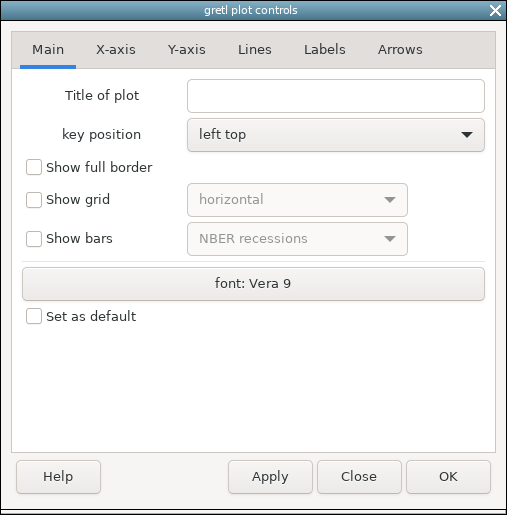
\includegraphics[scale=0.6]{figures/plot_control}
  \end{center}
  \caption{gretl's gnuplot controller}
  \label{fig-plot}
\end{figure}


\subsection{Publication-quality graphics: advanced options}
\label{plot-advanced}

The GUI plot editor has two limitations.  First, it cannot represent
all the myriad options that \app{gnuplot} offers. Users who are
sufficiently familiar with \app{gnuplot} to know what they're missing
in the plot editor presumably don't need much help from gretl,
so long as they can get hold of the \app{gnuplot} command file that
gretl has put together.  Second, even if the plot editor meets
your needs, in terms of fine-tuning the graph you see on screen, a few
details may need further work in order to get optimal results for
publication.

Either way, the first step in advanced tweaking of a graph is to get
access to the graph command file.

\begin{itemize}
\item In the graph display window, right-click and choose ``Save to
  session as icon''.
\item If it's not already open, open the icon view window---either
  via the menu item View/Icon view, or by clicking the ``session icon
  view'' button on the main-window toolbar.
\item Right-click on the icon representing the newly added graph and
  select ``Edit plot commands'' from the pop-up menu.
\item You get a window displaying the plot file
  (Figure~\ref{fig:plot-edit}).
\end{itemize}

\begin{figure}[htbp]
  \centering
  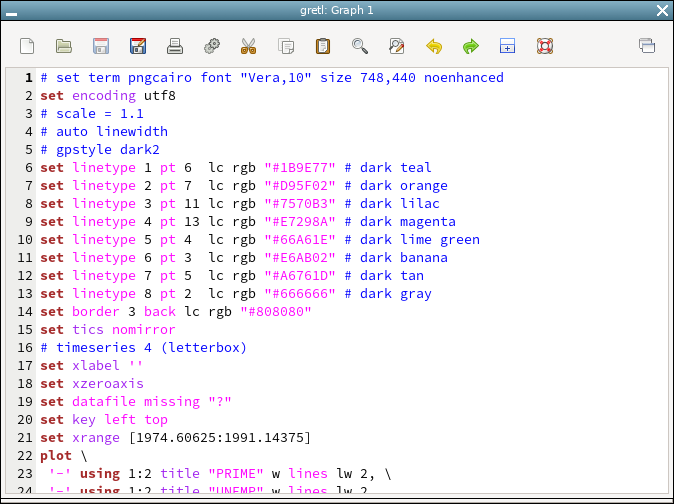
\includegraphics[scale=0.6]{figures/plotedit}
  \caption{Plot commands editor}
  \label{fig:plot-edit}
\end{figure}

Here are the basic things you can do in this window.  Obviously, you
can edit the file you just opened.  You can also send it for
processing by gnuplot, by clicking the ``Execute'' (cogwheel)
icon in the toolbar.  Or you can use the ``Save as'' button to save
a copy for editing and processing as you wish.

Unless you're a gnuplot expert, most likely you'll only need to edit a
couple of lines at the top of the file, specifying a driver (plus
options) and an output file.  We offer here a brief summary of some
points that may be useful.

First, \app{gnuplot}'s output mode is set via the command \texttt{set
  term} followed by the name of a supported driver (``terminal'' in
gnuplot parlance) plus various possible options.  (The top line in the
plot commands window shows the \texttt{set term} line that gretl
used to make a PNG file, commented out.)  The graphic formats that are
most suitable for publication are PDF and EPS.  These are supported by
the gnuplot \texttt{term} types \texttt{pdf}, \texttt{pdfcairo} and
\texttt{postscript} (with the \texttt{eps} option).  The
\texttt{pdfcairo} driver has the virtue that is behaves in a very
similar manner to the PNG one, the output of which you see on screen.
This is provided by the version of gnuplot that is included in the
gretl packages for MS Windows and Mac OS X; if you're on Linux
it may or may be supported.  If \texttt{pdfcairo} is not available,
the \texttt{pdf} terminal may be available; the \texttt{postscript}
terminal is almost certainly available.

Besides selecting a term type, if you want to get gnuplot to write the
actual output file you need to append a \texttt{set output} line
giving a filename.  Here are a few examples of the first two lines you
might type in the window editing your plot commands.  We'll make
these more ``realistic'' shortly.
%
\begin{code}
set term pdfcairo
set output 'mygraph.pdf'

set term pdf
set output 'mygraph.pdf'

set term postscript eps
set output 'mygraph.eps'
\end{code}

There are a couple of things worth remarking here.  First, you may
want to adjust the size of the graph, and second you may want to
change the font.  The default sizes produced by the above drivers are
5 inches by 3 inches for \texttt{pdfcairo} and \texttt{pdf}, and 5
inches by 3.5 inches for \texttt{postscript eps}.  In each case
you can change this by giving a size specification, which takes the
form \texttt{XX,YY} (examples below).  

You may ask, why bother changing the size in the gnuplot command file?
After all, PDF and EPS are both vector formats, so the graphs can be
scaled at will.  True, but a uniform scaling will also affect the font
size, which may end looking wrong.  You can get optimal results by
experimenting with the \texttt{font} and \texttt{size} options to
\app{gnuplot}'s \texttt{set term} command.  Here are some examples
(comments follow below).
%
\begin{code}
# pdfcairo, regular size, slightly amended
set term pdfcairo font "Sans,6" size 5in,3.5in
# or small size
set term pdfcairo font "Sans,5" size 3in,2in

# pdf, regular size, slightly amended
set term pdf font "Helvetica,8" size 5in,3.5in
# or small
set term pdf font "Helvetica,6" size 3in,2in

# postscript, regular 
set term post eps solid font "Helvetica,16"
# or small
set term post eps solid font "Helvetica,12" size 3in,2in
\end{code}

On the first line we set a sans serif font for \texttt{pdfcairo} at a
suitable size for a 5 $\times$ 3.5 inch plot (which you may find looks
better than the rather ``letterboxy'' default of 5 $\times$ 3).  And
on the second we illustrate what you might do to get a smaller 3
$\times$ 2 inch plot. You can specify the plot size in centimeters
if you prefer, as in
\begin{code}
set term pdfcairo font "Sans,6" size 6cm,4cm
\end{code}

We then repeat the exercise for the \texttt{pdf} terminal.  Notice
that here we're specifying one of the 35 standard PostScript fonts,
namely Helvetica.  Unlike \texttt{pdfcairo}, the plain \texttt{pdf}
driver is unlikely to be able to find fonts other than these.

In the third pair of lines we illustrate options for the
\texttt{postscript} driver (which, as you see, can be abbreviated as
\texttt{post}).  Note that here we have added the option
\texttt{solid}.  Unlike most other drivers, this one uses dashed lines
unless you specify the \texttt{solid} option.  Also note that we've
(apparently) specified a much larger font in this case.  That's
because the \texttt{eps} option in effect tells the
\texttt{postscript} driver to work at half-size (among other things),
so we need to double the font size.

Table~\ref{tab:drivers} summarizes the basics for the three drivers we
have mentioned.

\begin{table}[htbp]
  \centering
  \begin{tabular}{lcc}
    Terminal & default size (inches) & suggested font \\ [6pt]
    \texttt{pdfcairo} & 5 $\times$ 3 &   Sans,6 \\
    \texttt{pdf}      & 5 $\times$ 3 &   Helvetica,8 \\
    \texttt{post eps} & 5 $\times$ 3.5 & Helvetica,16 \\
  \end{tabular}
  \caption{Drivers for publication-quality graphics}
  \label{tab:drivers}
\end{table}

To find out more about \app{gnuplot} visit
\href{http://www.gnuplot.info/}{www.gnuplot.info}. This site has
documentation for the current version of the program in various
formats.

\subsection{Additional tips}
\label{subsect-graph-tips}

To be written.  Line widths, enhanced text.  Show a ``before and
after'' example.  

\section{Plotting graphs from scripts}
\label{sec:plotenv}

When working with scripts, you may want to have a graph shown onto
your display or saved into a file. In fact, if in your usual workflow
you find yourself creating similar graphs over and over again, you
might want to consider the option of writing a script which automates
this process for you. \app{Gretl} gives you two main tools for doing
this: one is a command called \cmd{gnuplot}, whose main use is to
create standard plot quickly. The other one is the \cmd{plot} command
block, which has a more elaborate syntax but offers you more control
on output.

\subsection{The \cmd{gnuplot} command}
\label{sec:gnuplot-cmd}

The \cmd{gnuplot} command is described at length in the \GCR\ and the
online help system. Here, we just summarize its main features:
basically, it consists of the \cmd{gnuplot} keyword, followed by a
list of items, telling the command \emph{what} you want plotted and a
list of options, telling it \emph{how} you want it plotted.

For example, the line
\begin{code}
gnuplot y1 y2 x   
\end{code}
will give you a basic XY plot of the two series \texttt{y1} and
\texttt{y2} on the vertical axis versus the series \texttt{x} on the
horizontal axis. In general, the arguments to the \cmd{gnuplot}
command is a list of series, the last of which goes on the x-axis,
while all the other ones go onto the y-axis. By default, the
\cmd{gnuplot} command gives you a scatterplot. If you just have one
variable on the y-axis, then \app{gretl} will also draw a the OLS
interpolation, if the fit is good enough.\footnote{The technical
  condition for this is that the two-tailed $p$-value for the slope
  coefficient should be under 10\%.}

Several aspects of the behavior described above can be modified. You
do this by appending options to the command. Most options can be
broadly grouped in three categories (FIXME: expand on this):
\begin{enumerate}
\item Plot styles
\item Algorithm for the fitted line
\item Input and output
\end{enumerate}

For more detail, consult the \GCR.

Example:

\begin{scode}
open AWM.gdt --quiet

# --- different styles -------

gnuplot PCR YER
gnuplot PCR YER --output=display
gnuplot PCR YER --output=display --time-series
gnuplot PCR YER --output=display --time-series --with-lines

# --- fitted lines -----------
# --- Phillips' curve --------

gnuplot INFQ URX  --output=display
gnuplot INFQ URX --suppress-fitted --output=display
gnuplot INFQ URX --inverse-fit --output=display
gnuplot INFQ URX --loess-fit --output=display
\end{scode}

FIXME: comment on the above

\subsection{The \cmd{plot} command block}
\label{sec:plotblock}

The \cmd{plot} environment is a way to pass information to Gnuplot in
a more structured way, so that customization of basic plot becomes
easier. It has the following characteristics:

The block starts with the \cmd{plot} keyword, followed by a required
parameter: the name of a list, a single series or a matrix. This
parameter specifies the data to be plotted. The starting line may be
prefixed with the \verb|savename <-| apparatus to save a plot as an icon
in the GUI program. The block ends with \cmd{end plot}.

Inside the block you have zero or more lines of these types, identified 
by an initial keyword:
\begin{description}
\item[\texttt{option}:] specify a single option (details below)
\item[\texttt{options}:] specify multiple options on a single line; if
  more than one option is given on a line, the options should be
  separated by spaces.
\item[\texttt{literal}:] a command to be passed to gnuplot literally 
\item[\texttt{printf}:] a printf statement whose result will be passed
  to gnuplot literally; this allows the use of string variables
  without having to resort to \verb!@!-style string substitution.
\end{description}

The options available are basically those of the current \cmd{gnuplot} 
command, but with a few differences. For one thing you don't need the 
leading double-dash in an "option" (or "options") line. Besides that,
\begin{itemize}
\item You can't use the option \option{matrix=whatever} with \cmd{plot}:
  that possibility is handled by providing the name of a matrix on the
  initial \cmd{plot} line.
\item The \option{input=filename} option is not supported: use
  \cmd{gnuplot} for the case where you're supplying the entire plot
  specification yourself.
\item The several options pertaining to the presence and type of a
  fitted line, are replaced in \cmd{plot} by a single option \cmd{fit} which
  requires a parameter. Supported values for the parameter are: none,
  linear, quadratic, cubic, inverse, semilog and loess. Example:
\begin{code}
  option fit=quadratic
\end{code}
\end{itemize}

As with \cmd{gnuplot}, the default is to show a linear fit in an X-Y scatter if 
it's significant at the 10 percent level.

Here's a simple example, the plot spec from the "bandplot" package,
which shows how to achieve the same result via the \cmd{command} and
the \cmd{plot} block, respectively:

\begin{code}
   gnuplot 1 2 3 4 --with-lines --matrix=plotmat \
   --suppress-fitted --output=display \
   { set linetype 3 lc rgb "#0000ff"; set title "@title"; \
     set nokey; set xlabel "@xname"; }
\end{code}

\begin{code}
   plot plotmat
     options with-lines fit=none
     literal set linetype 3 lc rgb "#0000ff"
     literal set nokey
     printf "set title \"%s\"", title
     printf "set xlabel \"%s\"", xname
   end plot --output=display
\end{code}

Note that \option{output=display} is appended to \cmd{end plot}; also
note that if you give a matrix to \cmd{plot} it's assumed you want to
plot all the columns. In addition, if you give a single series and the
dataset is time series, it's assumed you want a time-series plot.

FIXME: provide an example

\section{Boxplots}
\label{sect-boxplots}

\begin{figure}[htbp]
  \begin{center}
    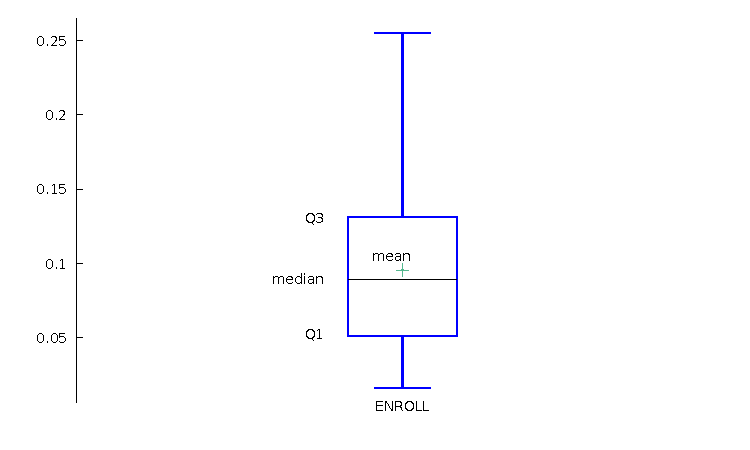
\includegraphics{figures/boxplot_sample}
  \end{center}
  \caption{Sample boxplot}
  \label{fig-boxplot}
\end{figure}

These plots (after Tukey and Chambers) display the distribution
of a variable. The central box encloses the middle 50 percent of the
data, i.e.\ it is bounded by the first and third quartiles.  The
``whiskers'' extend to the minimum and maximum values.  A line is
drawn across the box at the median and a ``\texttt{+}'' sign
identifies the mean---see Figure~\ref{fig-boxplot}.

In the case of boxplots with confidence intervals, dotted lines show
the limits of an approximate 90 percent confidence interval for the
median.  This is obtained by the bootstrap method, which can take a
while if the data series is very long. For details on constructing
boxplots, see the entry for \cmd{boxplot} in the \GCR\, or use the
\textsf{Help} button that appears when you select one of the boxplot
items under the menu item ``View, Graph specified vars'' in the main
gretl window.

\subsection{Factorized boxplots}

A nice feature which is quite useful for data visualization is the
conditional, or factorized boxplot.  This type of plot allows you to
examine the distribution of a variable conditional on the value of
some discrete factor.

As an example, we'll use one of the datasets supplied with
\app{gretl}, that is \cmd{rac3d}, which contains an example taken from
\cite{cameron-trivedi13} on the health conditions of 5190 people. The
script below compares the unconditional (marginal) distribution of the
number of illnesses in the past 2 weeks with the distribution of the
same variable, conditional on age classes.

\begin{scode}
open rac3d.gdt
# unconditional boxplot
boxplot ILLNESS --output=display
# create a discrete variable for age class: 
# 0 = below 20, 1 = bewteen 20 and 39, etc
series age_class = floor(AGE/0.2)
# conditional boxplot
boxplot ILLNESS age_class --factorized --output=display
\end{scode}

After running the code above, you should see two graphs similar to
Figure \ref{fig:fact-boxplots}. By comparing the marginal plot to
the factorized one, the effect of age on the mean number of illnesses
is quite evident (join the green crosses).

\begin{figure}[htbp]
  \centering
  \begin{tabular}{cc}
    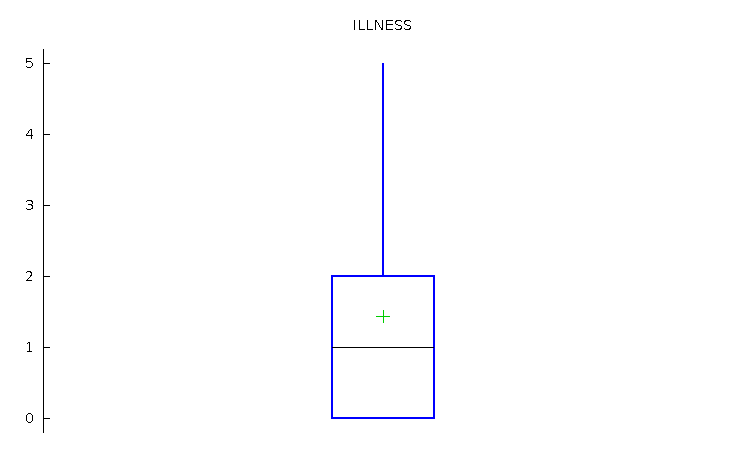
\includegraphics[width=0.475\textwidth]{figures/uboxplot} & 
    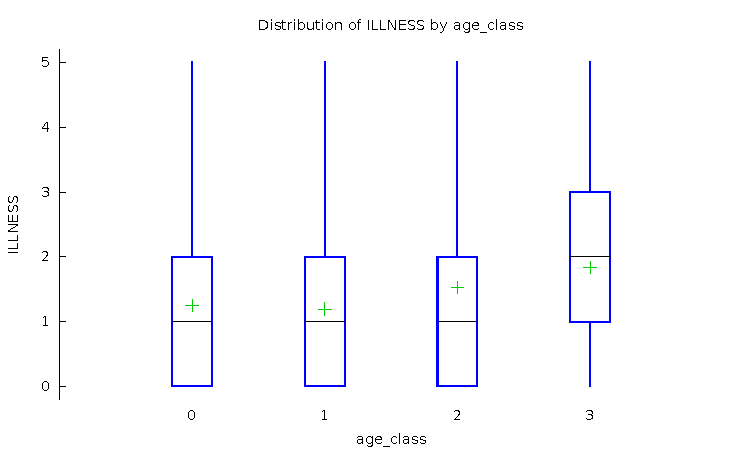
\includegraphics[width=0.475\textwidth]{figures/fboxplot}
  \end{tabular}
  \caption{Conditional and unconditional distribution of illnesses}
  \label{fig:fact-boxplots}
\end{figure}

%%% Local Variables: 
%%% mode: latex
%%% TeX-master: "gretl-guide"
%%% End: 


\chapter{Variabili discrete}
\label{chap-discrete}

Quando una variabile pu� assumere solo un numero finito, tipicamente basso, di
valori, essa si pu� chiamare \emph{discreta}. Alcuni comandi di
\app{gretl} si comportano in modo leggermente diverso quando sono usati su
variabili discrete; in pi�, \app{gretl} fornisce alcuni comandi che si applicano
solo alle variabili discrete.


\section{Dichiarazione delle variabili discrete}
\label{discr-declare}

Quando si crea un file di dati da zero, nessuna variabile viene considerata
discreta. Per marcare una variabile come discreta, � possibile agire in due
modi:
\begin{enumerate}
\item Dall'interfaccia grafica, selezionare ``Variabile, Modifica attributi''
  dal men�. Apparir� una finestra di dialogo che, se la variabile assume solo
  valori interi, contiene la casella ``Tratta questa variabile come discreta''.
  La stessa finestra di dialogo pu� essere richiamata dal men� contestuale
  (facendo clic col tasto destro su una variabile) o premendo il tasto F2;
\item Dall'interfaccia a riga di comando, usando il comando \texttt{discrete}.
  Il comando accetta uno o pi� argomenti, che possono essere variabili o liste
  di variabili. Ad esempio:
\begin{code}
  list xlist = x1 x2 x3
  discrete z1 xlist z2
\end{code}
In questo modo � possibile dichiarare pi� variabili discrete con un solo
comando, cosa che al momento non � possibile fare usando l'interfaccia grafica.
L'opzione \texttt{--reverse} inverte la dichiarazione, ossia rende continua una
variabile discreta.
Ad esempio:
\begin{code}
  discrete pippo
  # ora pippo � discreta
  discrete pippo --reverse
  # ora piipo � continua
\end{code}
\end{enumerate}

Si noti che marcare una variabile come discreta non ne modifica il contenuto. �
quindi responsabilit� dell'utente usare correttamente questa funzione. Per
ricodificare una variabile continua in classi, � possibile usare il comando
\texttt{genr} e le sue funzioni aritmetiche come nell'esempio seguente:
\begin{code}
  nulldata 100
  # genera una variabile con media 2 e varianza 1
  genr x = normal() + 2
  # suddivide in 4 classi
  genr z = (x>0) + (x>2) + (x>4)
  # ora dichiara z come discreta
  discrete z
\end{code}

Quando si marca una variabile come discreta, questa impostazione viene ricordata
dopo il salvataggio del file.

\section{Comandi per le variabili discrete}
\label{discr-commands}

\subsection{Il comando \texttt{dummify}}
\label{discr-dummify}

Il comando \texttt{dummify} prende come argomento una serie $x$ e crea delle
variabili dummy per ognuno dei valori distinti presenti in $x$, che deve essere
stata dichiarata discreta in precedenza. Ad esempio:
\begin{code}
  open greene22_2
  discrete Z5 # marca Z5 come discreta
  dummify Z5
\end{code}

L'effetto di questi comandi � quello di generare 5 nuove variabili dummy, i cui
nomi vanno da \texttt{DZ5\_1} fino a \texttt{DZ5\_5}, che corrispondono ai
diversi valori presenti in \texttt{Z5}. Ossia, la variabile
\texttt{DZ5\_4} vale 1 dove \texttt{Z5} vale 4, e 0 altrove. Questa funzionalit�
� disponibile anche nell'interfaccia grafica, con il comando del men�
``Aggiungi, dummy per le variabili discrete selezionate''.

Il comando \texttt{dummify} pu� essere usato anche con la sintassi seguente:
\begin{code}
  list dlist = dummify(x)
\end{code}
In questo modo, vengono create non solo le variabili dummy, ma anche una lista
che pu� essere usata in seguito (si veda la sezione~\ref{named-lists}).
L'esempio seguente calcola le statistiche descrittive per la variabile
\texttt{Y} in corrispondenza di ogni valore di \texttt{Z5}:
\begin{code}
  open greene22_2
  discrete Z5 # marca Z5 come discreta
  list foo = dummify(Z5)
  loop foreach i foo
    smpl $i --restrict --replace
    summary Y
  end loop
  smpl full
\end{code}
% $

Poich� \texttt{dummify} genera una lista, pu� essere usato direttamente in
comandi che accettano una lista come input, come \texttt{ols}.
Ad esempio:
\begin{code}
  open greene22_2
  discrete Z5 # marca Z5 come discreta
  ols Y 0 dummify(Z5)
\end{code}

\subsection{Il comando \texttt{freq}}
\label{discr-freq}

Il comando \texttt{freq} mostra le frequenze assolute e relative per una
variabile. Il modo in cui le frequenze vengono calcolate dipende dal carattere
discreto o continuo della variabile. Questo comando � disponibile anche
nell'interfaccia grafica, usando il comando del men� ``Variabile, Distribuzione
di frequenza''.

Per variabili discrete, le frequenze sono contate per ogni diverso valore
assunto dalla variabile. Per le variabili continue, i valori sono raggruppati in
``classi'' e quindi le frequenze sono calcolate per ogni classe.
Il numero di classi � calcolato in funzione del numero di osservazioni valide
nel campione selezionato al momento, come mostrato nella Tabella~\ref{tab:bins}.

\begin{table}[htbp]
  \centering
  \begin{tabular}{cc}
\hline
  Osservazioni & Classi \\
\hline
  $8 \le n < 16$ & 5 \\
  $16 \le n < 50 $ & 7 \\
  $50 \le n \le 850 $ & $\lceil \sqrt{n} \rceil$  \\
  $n > 850 $ & 29 \\
\hline
\end{tabular}
\caption{Numero di classi per varie ampiezze campionarie}
\label{tab:bins}
\end{table}

Ad esempio, il codice seguente
\begin{code}
  open greene19_1
  freq TUCE
  discrete TUCE # marca TUCE come discreta
  freq TUCE
\end{code}
produce questo risultato
\begin{code}
Lettura del file dati /usr/local/share/gretl/data/greene/greene19_1.gdt
Periodicit�: 1, oss. max.: 32,
Intervallo delle osservazioni: 1-32

5 variabili elencate:
  0) const    1) GPA      2) TUCE     3) PSI      4) GRADE  

? freq TUCE

Distribuzione di frequenza per TUCE, oss. 1-32
Numero di intervalli = 7, media = 21,9375, deviazione standard = 3,90151

       Intervallo        P.med.  Frequenza    Rel.     Cum.

          <  13,417     12,000        1      3,12%    3,12% *
    13,417 - 16,250     14,833        1      3,12%    6,25% *
    16,250 - 19,083     17,667        6     18,75%   25,00% ******
    19,083 - 21,917     20,500        6     18,75%   43,75% ******
    21,917 - 24,750     23,333        9     28,12%   71,88% **********
    24,750 - 27,583     26,167        7     21,88%   93,75% *******
          >= 27,583     29,000        2      6,25%  100,00% **

Test per l'ipotesi nulla di distribuzione normale:
Chi-quadro(2) = 1,872 con p-value 0,39211

? discrete TUCE # marca TUCE come discreta

? freq TUCE
Distribuzione di frequenza per TUCE, oss. 1-32

          Frequenza    Rel.     Cum.

  12           1      3,12%    3,12% *
  14           1      3,12%    6,25% *
  17           3      9,38%   15,62% ***
  19           3      9,38%   25,00% ***
  20           2      6,25%   31,25% **
  21           4     12,50%   43,75% ****
  22           2      6,25%   50,00% **
  23           4     12,50%   62,50% ****
  24           3      9,38%   71,88% ***
  25           4     12,50%   84,38% ****
  26           2      6,25%   90,62% **
  27           1      3,12%   93,75% *
  28           1      3,12%   96,88% *
  29           1      3,12%  100,00% *

Test per l'ipotesi nulla di distribuzione normale:
Chi-quadro(2) = 1,872 con p-value 0,39211
\end{code}
Come si pu� vedere dall'esempio, viene calcolato automaticamente un test
Jarque--Bera per la normalit�.

Questo comando accetta due opzioni: \texttt{--quiet}, per evitare la stampa
dell'istogramma, e \texttt{--gamma}, per sostituire il test di normalit� con
il test non parametrico di Locke, la cui ipotesi nulla � che i dati seguano una
distribuzione Gamma.


\subsection{Il comando \texttt{xtab}}
\label{discr-xtab}

Il comando \texttt{xtab} ha la sintassi seguente
\begin{code}
  xtab lista-y ; lista-x
\end{code}
dove \texttt{lista-y} e \texttt{lista-x} sono liste di variabili discrete;
esso produce tabulazioni incrociate per ognuna delle variabili nella
\texttt{lista-y} (per riga) rispetto a ognuna delle variabili nella
\texttt{lista-x} (per colonna). Al momento, questa funzionalit� non �
accessibile dall'interfaccia grafica.

Ad esempio:
\begin{code}
  open greene22_2
  discrete Z* # Marca Z1-Z8 come discrete
  xtab Z1 Z4 ; Z5 Z6
\end{code}
produce questo risultato
\begin{code}
Tabulazione incrociata di Z1 (righe) rispetto a Z5 (colonne)

       [   1][   2][   3][   4][   5]  TOT.
  
[   0]    20    91    75    93    36    315
[   1]    28    73    54    97    34    286

TOTALE    48   164   129   190    70    601

Test chi-quadro di Pearson = 5,48233 (4 df, p-value = 0,241287)

Tabulazione incrociata di Z1 (righe) rispetto a Z6 (colonne)

       [   9][  12][  14][  16][  17][  18][  20]  TOT.
  
[   0]     4    36   106    70    52    45     2    315
[   1]     3     8    48    45    37    67    78    286

TOTALE     7    44   154   115    89   112    80    601

Test chi-quadro di Pearson = 123,177 (6 df, p-value = 3,50375e-24)

Tabulazione incrociata di Z4 (righe) rispetto a Z5 (colonne)

       [   1][   2][   3][   4][   5]  TOT.
  
[   0]    17    60    35    45    14    171
[   1]    31   104    94   145    56    430

TOTALE    48   164   129   190    70    601

Test chi-quadro di Pearson = 11,1615 (4 df, p-value = 0,0248074)

Tabulazione incrociata di Z4 (righe) rispetto a Z6 (colonne)

       [   9][  12][  14][  16][  17][  18][  20]  TOT.
  
[   0]     1     8    39    47    30    32    14    171
[   1]     6    36   115    68    59    80    66    430

TOTALE     7    44   154   115    89   112    80    601

Test chi-quadro di Pearson = 18,3426 (6 df, p-value = 0,0054306)
\end{code}

Il test $\chi^2$ di Pearson per l'indipendenza viene mostrato automaticamente
se la frequenza attesa nell'ipotesi di indipendenza supera 5 per almeno l'80 per
cento delle celle. L'opzione \texttt{--chi-square} fa in modo che il test venga
sempre mostrato.

Inoltre, le opzioni \texttt{--row} o \texttt{--column} fanno in modo che vengano
mostrate le percentuali di riga o di colonna.

Se si vuole incollare il risultato di \texttt{xtab} in qualche altra
applicazione, ad esempio un foglio di calcolo, � utile usare l'opzione
\texttt{--zeros}, che scrive il numero zero nelle celle con frequenza pari a
zero, invece di lasciarle vuote.

%%% Local Variables: 
%%% mode: latex
%%% TeX-master: "gretl-guide"
%%% End: 

\chapter{Loop constructs}
\label{chap:looping}

\section{Introduction}
\label{loop-intro}

The command \cmd{loop} opens a special mode in which \app{gretl}
accepts a block of commands to be repeated zero or more times.  This
feature may be useful for, among other things, Monte Carlo simulations,
bootstrapping of test statistics and iterative estimation procedures.
The general form of a loop is:

\begin{code}
loop control-expression [ --progressive | --verbose | --quiet ]
   loop body
endloop
\end{code}

Five forms of control-expression are available, as explained in
section~\ref{loop-control}.

Not all \app{gretl} commands are available within loops.  The commands
that are not presently accepted in this context are shown in
Table~\ref{tab:nonloopcmds}.

\begin{table}[htbp]
\caption{Commands not usable in loops}
\label{tab:nonloopcmds}
\begin{center}
%% The following is generated automatically
\input tabnonloopcmds.tex
\end{center}
\end{table}

By default, the \cmd{genr} command operates quietly in the context of
a loop (without printing information on the variable generated).  To
force the printing of feedback from \cmd{genr} you may specify the
\option{verbose} option to \cmd{loop}.  The \option{quiet} option
suppresses the usual printout of the number of iterations performed,
which may be desirable when loops are nested.

The \option{progressive} option to \cmd{loop} modifies the behavior of
the commands \cmd{print} and \cmd{store}, and certain estimation
commands, in a manner that may be useful with Monte Carlo analyses
(see Section \ref{loop-progressive}).
    
The following sections explain the various forms of the loop control
expression and provide some examples of use of loops.  

\tip{If you are carrying out a substantial Monte Carlo analysis with
  many thousands of repetitions, memory capacity and processing time
  may be an issue.  To minimize the use of computer resources, run
  your script using the command-line program, \app{gretlcli}, with
  output redirected to a file.}

\section{Loop control variants}
\label{loop-control}

\subsection{Count loop}
\label{loop-count}

The simplest form of loop control is a direct specification of the
number of times the loop should be repeated.  We refer to this as a
``count loop''.  The number of repetitions may be a numerical
constant, as in \verb+loop 1000+, or may be read from a scalar
variable, as in \verb+loop replics+.

In the case where the loop count is given by a variable, say
\verb+replics+, in concept \verb+replics+ is an integer; if the value
is not integral, it is converted to an integer by truncation.  Note
that \verb+replics+ is evaluated only once, when the loop is initially
compiled.
      

\subsection{While loop}
\label{loop-while}

A second sort of control expression takes the form of the keyword
\cmd{while} followed by a boolean expression.  For example,
%
\begin{code}
loop while essdiff > .00001
\end{code}

Execution of the commands within the loop will continue so long as (a)
the specified condition evaluates as true and (b) the number of
iterations does not exceed the value of the internal variable
\verb|loop_maxiter|.  By default this equals 250, but you can specify
a different value via the \cmd{set} command (see the \GCR).

\subsection{Index loop}
\label{loop-index}

A third form of loop control uses an index variable, for example
\verb+i+.\footnote{It is common programming practice to use simple,
  one-character names for such variables.  However, you may use any
  name that is acceptable by gretl: up to 15 characters, starting with
  a letter, and containing nothing but letters, numerals and the
  underscore character.}  In this case you specify starting and ending
values for the index, which is incremented by one each time round the
loop.  The syntax looks like this: \cmd{loop i=1..20}.

The index variable may be a pre-existing scalar; if this is not the
case, the variable is created automatically and is destroyed on exit
from the loop.

The index may be used within the loop body in either of two ways: you
can access the integer value of \verb+i+ (see Example
\ref{loop-panel-script}) or you can use its string representation,
\dollar{i} (see Example \ref{loop-string-script}).

The starting and ending values for the index can be given in numerical
form, or by reference to predefined scalar variables.  In the latter
case the variables are evaluated once, at the start of the loop.  In
addition, with time series data you can give the starting and ending
values in the form of dates, as in \cmd{loop i=1950:1..1999:4}.

This form of loop control is intended to be quick and easy, and as
such it is subject to certain limitations.  You cannot do arithmetic
within the loop control expression, as in
\begin{code}
loop i=k..2*k # won't work
\end{code}
But one extension is permitted for convenience: you can inflect a loop
control variable with a minus sign, as in
\begin{code}
loop k=-lag..lag # OK
\end{code}

Also note that in this sort of loop the index variable is always
incremented by one at each iteration.  If, for example, you have
\begin{code}
loop i=m..n
\end{code}
where \texttt{m} and \texttt{n} are scalar variables with values
\texttt{m} $>$ \texttt{n} at the time of execution, the index will not
be decremented; rather, the loop will simply be bypassed.

If you need more complex loop control, see the ``\texttt{for}'' form
below.

The index loop is particularly useful in conjunction with the
\texttt{values()} matrix function when some operation must be carried
out for each value of some discrete variable (see chapter
\ref{chap:discrete}). Consider the following example:

\begin{code}
open greene22_2
discrete Z8
v8 = values(Z8)
n = rows(v8)
loop i=1..n
  scalar xi = v8[i]
  smpl (Z8=xi) --restrict --replace
  printf "mean(Y | Z8 = %g) = %8.5f, sd(Y | Z8 = %g) = %g\n", \
    xi, mean(Y), xi, sd(Y)
endloop
\end{code}

In this case, we evaluate the conditional mean and standard deviation
of the variable \texttt{Y} for each value of \texttt{Z8}.

\subsection{Foreach loop}
\label{loop-each}

The fourth form of loop control also uses an index variable, in this
case to index a specified list of strings.  The loop is executed once
for each string in the list.  This can be useful for performing
repetitive operations on a list of variables.  Here is an example of
the syntax:
      
\begin{code}
loop foreach i peach pear plum
   print "$i"
endloop
\end{code}

This loop will execute three times, printing out ``peach'', ``pear''
and ``plum'' on the respective iterations.  The numerical value of
the index starts at 1 and is incremented by 1 at each iteration.

If you wish to loop across a list of variables that are contiguous in
the dataset, you can give the names of the first and last variables in
the list, separated by ``\verb+..+'', rather than having to type all
the names.  For example, say we have 50 variables \verb+AK+,
\verb+AL+, \dots{}, \verb+WY+, containing income levels for the states
of the US.  To run a regression of income on time for each of the
states we could do:

\begin{code}
genr time
loop foreach i AL..WY
   ols $i const time
endloop
\end{code}

This loop variant can also be used for looping across the elements in
a \textit{named list} (see chapter~\ref{chap-persist}).  For example:

\begin{code}
list ylist = y1 y2 y3
loop foreach i ylist
   ols $i const x1 x2
endloop
\end{code}

Note that if you use this idiom inside a function (see
chapter~\ref{chap:functions}), looping across a list that has been
supplied to the function as an argument, it is necessary to use the
syntax \textsl{listname}.\dollar{i} to reference the list-member
variables.  In the context of the example above, this would mean
replacing the third line with
%
\begin{code}
   ols ylist.$i const x1 x2
\end{code}

\subsection{For loop}
\label{loop-for}

The final form of loop control emulates the \cmd{for} statement in the
C programming language.  The sytax is \texttt{loop for}, followed by
three component expressions, separated by semicolons and surrounded by
parentheses.  The three components are as follows:

\begin{enumerate}
\item Initialization: This is evaluated only once, at the start of the
  loop.  Common example: setting a scalar control variable to some
  starting value.
\item Continuation condition: this is evaluated at the top of each
  iteration (including the first).  If the expression evaluates as
  true (non-zero), iteration continues, otherwise it stops. Common
  example: an inequality expressing a bound on a control variable.
\item Modifier: an expression which modifies the value of
  some variable.  This is evaluated prior to checking the
  continuation condition, on each iteration after the first.
  Common example: a control variable is incremented or
  decremented.
\end{enumerate}

Here's a simple example:
%
\begin{code}
loop for (r=0.01; r<.991; r+=.01)
\end{code}

In this example the variable \verb+r+ will take on the values 0.01,
0.02, \dots{}, 0.99 across the 99 iterations.  Note that due to the
finite precision of floating point arithmetic on computers it may be
necessary to use a continuation condition such as the above,
\verb+r<.991+, rather than the more ``natural'' \verb+r<=.99+.  (Using
double-precision numbers on an x86 processor, at the point where you
would expect \verb+r+ to equal 0.99 it may in fact have value
0.990000000000001.)

Any or all of the three expressions governing a \texttt{for} loop may
be omitted --- the minimal form is \texttt{(;;)}.  If the continuation
test is omitted it is implicitly true, so you have an infinite loop
unless you arrange for some other way out, such as a \cmd{break}
statement.

If the initialization expression in a \texttt{for} loop takes the
common form of setting a scalar variable to a given value, the string
representation of that scalar's value is made available within
the loop via the accessor \dollar{\emph{varname}}.  


\section{Progressive mode}
\label{loop-progressive}

If the \option{progressive} option is given for a command loop,
special behavior is invoked for certain commands, namely, \cmd{print},
\cmd{store} and simple estimation commands.  By ``simple'' here we
mean commands which (a) estimate a single equation (as opposed to a
system of equations) and (b) do so by means of a single command
statement (as opposed to a block of statements, as with \cmd{nls} and
\cmd{mle}).  The paradigm is \cmd{ols}; other possibilities include
\cmd{tsls}, \cmd{wls}, \cmd{logit} and so on.

The special behavior is as follows.

Estimators: The results from each individual iteration of the
estimator are not printed.  Instead, after the loop is completed you
get a printout of (a) the mean value of each estimated coefficient
across all the repetitions, (b) the standard deviation of those
coefficient estimates, (c) the mean value of the estimated standard
error for each coefficient, and (d) the standard deviation of the
estimated standard errors.  This makes sense only if there is some
random input at each step.

\cmd{print}: When this command is used to print the value of a
variable, you do not get a print each time round the loop.  Instead,
when the loop is terminated you get a printout of the mean and
standard deviation of the variable, across the repetitions of the
loop.  This mode is intended for use with variables that have a scalar
value at each iteration, for example the error sum of squares from a
regression.  Data series cannot be printed in this way, and neither
can matrices.

\cmd{store}: This command writes out the values of the specified
scalars, from each time round the loop, to a specified file.  Thus it
keeps a complete record of their values across the iterations.  For
example, coefficient estimates could be saved in this way so as to
permit subsequent examination of their frequency distribution.  Only
one such \cmd{store} can be used in a given loop.

\section{Loop examples}
\label{loop-examples}


\subsection{Monte Carlo example}
\label{loop-mc-example}

A simple example of a Monte Carlo loop in ``progressive'' mode is
shown in Example~\ref{monte-carlo-loop}.

\begin{script}[htbp]
  \caption{Simple Monte Carlo loop}
  \label{monte-carlo-loop}
\begin{scode}
nulldata 50
set seed 547
genr x = 100 * uniform()
# open a "progressive" loop, to be repeated 100 times
loop 100 --progressive
   genr u = 10 * normal()
   # construct the dependent variable
   genr y = 10*x + u
   # run OLS regression
   ols y const x
   # grab the coefficient estimates and R-squared
   genr a = $coeff(const)
   genr b = $coeff(x)
   genr r2 = $rsq
   # arrange for printing of stats on these
   print a b r2
   # and save the coefficients to file
   store coeffs.gdt a b
endloop
\end{scode}
\end{script}

This loop will print out summary statistics for the `a' and `b'
estimates and $R^2$ across the 100 repetitions.  After running the
loop, \verb+coeffs.gdt+, which contains the individual coefficient
estimates from all the runs, can be opened in \app{gretl} to examine
the frequency distribution of the estimates in detail.

The command \cmd{nulldata} is useful for Monte Carlo work.  Instead of
opening a ``real'' data set, \cmd{nulldata 50} (for instance) opens a
dummy data set, containing just a constant and an index variable, with
a series length of 50. Constructed variables can then be added using
the \cmd{genr} command.  See the \cmd{set} command for information on
generating repeatable pseudo-random series.

\subsection{Iterated least squares}
\label{loop-ils-examples}

Example \ref{greene-ils-script} uses a ``while'' loop to replicate the
estimation of a nonlinear consumption function of the form
	
\[ C = \alpha + \beta Y^{\gamma} + \epsilon \]

as presented in \cite{greene00}, Example 11.3.  This script is included
in the \app{gretl} distribution under the name \verb+greene11_3.inp+;
you can find it in \app{gretl} under the menu item ``File, Script files,
Practice file, Greene...''.

The option \option{print-final} for the \cmd{ols} command arranges
matters so that the regression results will not be printed each time
round the loop, but the results from the regression on the last
iteration will be printed when the loop terminates.

\begin{script}[htbp]
  \caption{Nonlinear consumption function}
  \label{greene-ils-script}
\begin{scode}
open greene11_3.gdt
# run initial OLS
ols C 0 Y
genr essbak = $ess
genr essdiff = 1
genr beta = $coeff(Y)
genr gamma = 1
# iterate OLS till the error sum of squares converges
loop while essdiff > .00001
   # form the linearized variables
   genr C0 = C + gamma * beta * Y^gamma * log(Y)
   genr x1 = Y^gamma
   genr x2 = beta * Y^gamma * log(Y)
   # run OLS 
   ols C0 0 x1 x2 --print-final --no-df-corr --vcv
   genr beta = $coeff(x1)
   genr gamma = $coeff(x2)
   genr ess = $ess
   genr essdiff = abs(ess - essbak)/essbak
   genr essbak = ess
endloop 
# print parameter estimates using their "proper names"
set echo off
printf "alpha = %g\n", $coeff(0)
printf "beta  = %g\n", beta
printf "gamma = %g\n", gamma
\end{scode}
\end{script}

Example~\ref{jack-arma} shows how a loop can be used to
estimate an ARMA model, exploiting the ``outer product of the
gradient'' (OPG) regression discussed by Davidson and MacKinnon in
their \emph{Estimation and Inference in Econometrics}.

\begin{script}[htbp]
  \caption{ARMA 1, 1}
  \label{jack-arma}
\begin{scode}
open armaloop.gdt

genr c = 0
genr a = 0.1
genr m = 0.1

series e = 1.0
genr de_c = e
genr de_a = e
genr de_m = e

genr crit = 1
loop while crit > 1.0e-9

   # one-step forecast errors
   genr e = y - c - a*y(-1) - m*e(-1)  

   # log-likelihood 
   genr loglik = -0.5 * sum(e^2)
   print loglik

   # partials of forecast errors wrt c, a, and m
   genr de_c = -1 - m * de_c(-1) 
   genr de_a = -y(-1) -m * de_a(-1)
   genr de_m = -e(-1) -m * de_m(-1)

   # partials of l wrt c, a and m
   genr sc_c = -de_c * e
   genr sc_a = -de_a * e
   genr sc_m = -de_m * e

   # OPG regression
   ols const sc_c sc_a sc_m --print-final --no-df-corr --vcv

   # Update the parameters
   genr dc = $coeff(sc_c) 
   genr c = c + dc
   genr da = $coeff(sc_a) 
   genr a = a + da
   genr dm = $coeff(sc_m) 
   genr m = m + dm

   printf "  constant        = %.8g (gradient = %#.6g)\n", c, dc
   printf "  ar1 coefficient = %.8g (gradient = %#.6g)\n", a, da
   printf "  ma1 coefficient = %.8g (gradient = %#.6g)\n", m, dm

   genr crit = $T - $ess
   print crit
endloop

genr se_c = $stderr(sc_c)
genr se_a = $stderr(sc_a)
genr se_m = $stderr(sc_m)

set echo off
printf "\n"
printf "constant = %.8g (se = %#.6g, t = %.4f)\n", c, se_c, c/se_c
printf "ar1 term = %.8g (se = %#.6g, t = %.4f)\n", a, se_a, a/se_a
printf "ma1 term = %.8g (se = %#.6g, t = %.4f)\n", m, se_m, m/se_m
\end{scode}
\end{script}


\subsection{Indexed loop examples}

Example \ref{loop-panel-script} shows an indexed loop in which the
\cmd{smpl} is keyed to the index variable \verb+i+.  Suppose we have a
panel dataset with observations on a number of hospitals for the years
1991 to 2000 (where the year of the observation is indicated by a
variable named \verb+year+).  We restrict the sample to each of these
years in turn and print cross-sectional summary statistics for
variables 1 through 4.

\begin{script}[htbp]
  \caption{Panel statistics}
  \label{loop-panel-script}
\begin{scode}
open hospitals.gdt
loop i=1991..2000
  smpl (year=i) --restrict --replace
  summary 1 2 3 4
endloop
\end{scode}
\end{script}


Example \ref{loop-string-script} illustrates string substitution in an
indexed loop.

\begin{script}[htbp]
  \caption{String substitution}
  \label{loop-string-script}
\begin{scode}
open bea.dat
loop i=1987..2001
  genr V = COMP$i
  genr TC = GOC$i - PBT$i
  genr C = TC - V
  ols PBT$i const TC V
endloop
\end{scode}
\end{script}

The first time round this loop the variable \verb+V+ will be set to
equal \verb+COMP1987+ and the dependent variable for the \cmd{ols}
will be \verb+PBT1987+. The next time round \verb+V+ will be redefined
as equal to \verb+COMP1988+ and the dependent variable in the
regression will be \verb+PBT1988+.  And so on.

%%% Local Variables: 
%%% mode: latex
%%% TeX-master: "gretl-guide"
%%% End: 


\chapter{User-defined functions}
\label{chap:functions}

\section{Defining a function}
\label{func-define}

\app{Gretl} offers a mechanism for defining functions, which may be
called via the command line, in the context of a script, or (if
packaged appropriately, see section~\ref{sec:func-packages}) via the
program's graphical interface.

The syntax for defining a function looks like this:\footnote{The
  syntax given here differs from the standard prior to \app{gretl}
  version 1.8.4.  For reasons of backward compatibility the old syntax
  is still supported; see section~\ref{sec:old-func} for details.}

\begin{raggedright}
\texttt{function} \textsl{return-type} \textsl{function-name}
\texttt{(}\textsl{parameters}\texttt{)} \\
\qquad  \textsl{function body} \\
\texttt{end function}
\end{raggedright}

The opening line of a function definition contains these elements, in
strict order:

\begin{enumerate}
\item The keyword \texttt{function}.
\item \textsl{return-type}, which states the type of value returned by
  the function, if any.  This must be one of \texttt{void} (if the
  function does not return anything), \texttt{scalar},
  \texttt{series}, \texttt{matrix}, \texttt{list} or \texttt{string}.
\item \textsl{function-name}, the unique identifier for the
  function.  Names must start with a letter. They have a maximum
  length of 31 characters; if you type a longer name it will be
  truncated.  Function names cannot contain spaces.  You will get an
  error if you try to define a function having the same name as an
  existing \app{gretl} command.
\item The functions's \textsl{parameters}, in the form of a
  comma-separated list enclosed in parentheses.  This may be run
  into the function name, or separated by white space as shown.
\end{enumerate}

Function parameters can be of any of the types shown
below.\footnote{An additional parameter type is available for GUI use,
  namely \texttt{obs}; this is equivalent to \texttt{int} except for
  the way it is represented in the graphical interface for calling a
  function.}

\begin{center}
\begin{tabular}{ll}
\multicolumn{1}{c}{Type} & 
\multicolumn{1}{c}{Description} \\ [4pt]
\texttt{bool}   & scalar variable acting as a Boolean switch \\
\texttt{int}    & scalar variable acting as an integer  \\
\texttt{scalar} & scalar variable \\
\texttt{series} & data series \\
\texttt{list}   & named list of series \\
\texttt{matrix} & matrix or vector \\
\texttt{string} & string variable or string literal \\
\texttt{bundle} & all-purpose container (see section~\ref{sec:Bundles})
\end{tabular}
\end{center}

Each element in the listing of parameters must include two terms: a
type specifier, and the name by which the parameter shall be known
within the function.  An example follows:
%    
\begin{code}
function scalar myfunc (series y, list xvars, bool verbose)
\end{code}

Each of the type-specifiers, with the exception of \texttt{list} and
\texttt{string}, may be modified by prepending an asterisk to the
associated parameter name, as in
%    
\begin{code}
function scalar myfunc (series *y, scalar *b)
\end{code}

The meaning of this modification is explained below (see section
\ref{funscope}); it is related to the use of pointer arguments in the
C programming language.

\subsection{Function parameters: optional refinements}

Besides the required elements mentioned above, the specification of a
function parameter may include some additional fields, as follows:
\begin{itemize}
\item The \texttt{const} modifier.
\item For \texttt{scalar} or \texttt{int} parameters: minimum, maximum
  and default values; or for \texttt{bool} parameters, just a default
  value.
\item For all parameters, a descriptive string.
\item For \texttt{int} parameters with minimum and maximum values
  specified, a set of strings to associate with the allowed numerical
  values (value labels).
\end{itemize}

The first two of these options may be useful in many contexts; the
last two may be helpful if a function is to be packaged for use in
the \app{gretl} GUI (but probably not otherwise). We now expand on
each of the options.

\begin{itemize}

\item The \texttt{const} modifier: must be given as a prefix to the
  basic parameter specification, as in
%    
\begin{code}
const matrix M
\end{code} 
%
This constitutes a promise that the corresponding argument will not be
modified within the function; \app{gretl} will flag an error if
the function attempts to modify the argument.

\item Minimum, maximum and default values for \texttt{scalar} or
  \texttt{int} types: These values should directly follow the name of
  the parameter, enclosed in square brackets and with the individual
  elements separated by colons.  For example, suppose we have an
  integer parameter \texttt{order} for which we wish to specify a
  minimum of 1, a maximum of 12, and a default of 4.  We can write
%    
\begin{code}
int order[1:12:4]
\end{code} 
%
If you wish to omit any of the three specifiers, leave the
corresponding field empty.  For example \texttt{[1::4]} would specify
a minimum of 1 and a default of 4 while leaving the maximum
unlimited.  

For a parameter of type \texttt{bool} (whose values are just zero or
non-zero), you can specify a default of 1 (true) or 0 (false), as in
%    
\begin{code}
bool verbose[0]
\end{code} 

\item Descriptive string: This will show up as an aid to the user if
  the function is packaged (see section~\ref{sec:func-packages} below)
  and called via \app{gretl}'s graphical interface.  The string should
  be enclosed in double quotes and separated from the preceding
  elements of the parameter specification with a space, as in
%
\begin{code}
series y "dependent variable"
\end{code} 

\item Value labels: These may be used only with \texttt{int}
  parameters for which minimum and maximum values have been specified,
  so there is a fixed number of admissible values, and the number of
  labels must match the number of values. They will show up in the
  graphical interface in the form of a drop-down list, making the
  function writer's intent clearer when an integer argument represents
  a categorical selection. A set of value labels must be enclosed in
  braces, and the individual labels must be enclosed in double quotes
  and separated by commas or spaces.  For example:
%
\begin{code}
int case[1:3:1] {"Fixed effects", "Between model", "Random effects"}
\end{code} 

\end{itemize}

If two or more of the trailing optional fields are given in a
parameter specification, they must be given in the order shown above:
min--max--default, description, value labels. Note that there is no
facility for ``escaping'' characters within descriptive strings or
value labels; these may contain spaces but they cannot contain the
double-quote character.  

Here is an example of a well-formed function specification using all
the elements mentioned above:
%
\begin{code}
function matrix myfunc (series y "dependent variable",
                        list X "regressors",
                        int p[0::1] "lag order",
                        int c[1:2:1] "criterion" {"AIC", "BIC"},
                        bool quiet[0])
\end{code} 

One advantage of specifying default values for parameters, where
applicable, is that in script or command-line mode users may omit
trailing arguments that have defaults. For example, \texttt{myfunc}
above could be invoked with just two arguments, corresponding to
\texttt{y} and \texttt{X}; implicitly \texttt{p} = 1, \texttt{c} = 1
and \texttt{quiet} is false.

\subsection{Functions taking no parameters}

You may define a function that has no parameters (these are called
``routines'' in some programming languages).  In this case,  
use the keyword \texttt{void} in place of the listing of parameters:
%    
\begin{code}
function matrix myfunc2 (void)
\end{code}


\subsection{The function body}
   
The \textsl{function body} is composed of \app{gretl} commands, or
calls to user-defined functions (that is, function calls may be
nested).  A function may call itself (that is, functions may be
recursive). While the function body may contain function calls, it may
not contain function definitions.  That is, you cannot define a
function inside another function.  For further details, see
section~\ref{func-details}.


\section{Calling a function}
\label{func-call}

A user function is called by typing its name followed by zero or more
arguments enclosed in parentheses.  If there are two or more arguments
these should be separated by commas.  

There are automatic checks in place to ensure that the number of
arguments given in a function call matches the number of parameters,
and that the types of the given arguments match the types specified in
the definition of the function.  An error is flagged if either of
these conditions is violated.  One qualification: allowance is made
for omitting arguments at the end of the list, provided that default
values are specified in the function definition.  To be precise, the
check is that the number of arguments is at least equal to the number
of \textit{required} parameters, and is no greater than the total
number of parameters.

A scalar, series or matrix argument to a function may be given either
as the name of a pre-existing variable or as an expression which
evaluates to a variable of the appropriate type.  Scalar arguments may
also be given as numerical values.  List arguments must be specified
by name.

The following trivial example illustrates a function call that
correctly matches the function definition.
    
\begin{code}
# function definition
function scalar ols_ess(series y, list xvars)
  ols y 0 xvars --quiet
  scalar myess = $ess
  printf "ESS = %g\n", myess
  return myess
end function
# main script
open data4-1
list xlist = 2 3 4
# function call (the return value is ignored here)
ols_ess(price, xlist)
\end{code}

The function call gives two arguments: the first is a data series
specified by name and the second is a named list of regressors.  Note
that while the function offers the variable \verb+myess+ as a return
value, it is ignored by the caller in this instance.  (As a side note
here, if you want a function to calculate some value having to do with
a regression, but are not interested in the full results of the
regression, you may wish to use the \option{quiet} flag with the
estimation command as shown above.)
    
A second example shows how to write a function call that assigns
a return value to a variable in the caller:
    
\begin{code}
# function definition
function series get_uhat(series y, list xvars)
  ols y 0 xvars --quiet
  series uh = $uhat
  return uh
end function
# main script
open data4-1
list xlist = 2 3 4
# function call
series resid = get_uhat(price, xlist)
\end{code}

\section{Deleting a function}
\label{func-del}

If you have defined a function and subsequently wish to clear it out
of memory, you can do so using the keywords \texttt{delete} or
\texttt{clear}, as in

\begin{code}
function myfunc delete
function get_uhat clear
\end{code}

Note, however, that if \texttt{myfunc} is already a defined function,
providing a new definition automatically overwrites the previous one,
so it should rarely be necessary to delete functions explicitly.

\section{Function programming details}
\label{func-details}

\subsection{Variables versus pointers}
\label{funscope}

Series, scalar, and matrix arguments to functions can be passed in two
ways: ``as they are'', or as pointers. For example, consider the
following:
\begin{code}
function series triple1(series x)
  return 3*x
end function
  
function series triple2(series *x)
  return 3*x
end function
\end{code}

These two functions are nearly identical (and yield the same result);
the only difference is that you need to feed a series into
\texttt{triple1}, as in \texttt{triple1(myseries)}, while
\texttt{triple2} must be supplied a \emph{pointer} to a series, as in
\texttt{triple2(\&myseries)}. 

Why make the distinction? There are two main reasons for doing so:
modularity and performance.

By modularity we mean the insulation of a function from the rest of
the script which calls it.  One of the many benefits of this approach
is that your functions are easily reusable in other contexts.  To
achieve modularity, \emph{variables created within a function are
  local to that function, and are destroyed when the function exits},
unless they are made available as return values and these values are
``picked up'' or assigned by the caller.
    
In addition, functions do not have access to variables in ``outer
scope'' (that is, variables that exist in the script from which the
function is called) except insofar as these are explicitly passed to
the function as arguments.

By default, when a variable is passed to a function as an argument,
what the function actually ``gets'' is a \emph{copy} of the outer
variable, which means that the value of the outer variable is not
modified by anything that goes on inside the function.  But the use of
pointers allows a function and its caller to cooperate such that
an outer variable can be modified by the function.  In effect, this
allows a function to ``return'' more than one value (although only one
variable can be returned directly --- see below).  The parameter in
question is marked with a prefix of \texttt{*} in the function
definition, and the corresponding argument is marked with the
complementary prefix \verb+&+ in the caller.  For example,
%
\begin{code}
function series get_uhat_and_ess(series y, list xvars, scalar *ess)
  ols y 0 xvars --quiet
  ess = $ess
  series uh = $uhat
  return uh
end function
# main script
open data4-1
list xlist = 2 3 4
# function call
scalar SSR
series resid = get_uhat_and_ess(price, xlist, &SSR)
\end{code}
%
In the above, we may say that the function is given the \emph{address}
of the scalar variable \texttt{SSR}, and it assigns a value to that
variable (under the local name \texttt{ess}).  (For anyone used to
programming in C: note that it is not necessary, or even possible, to
``dereference'' the variable in question within the function using the
\texttt{*} operator.  Unadorned use of the name of the variable is
sufficient to access the variable in outer scope.)

An ``address'' parameter of this sort can be used as a means of
offering optional information to the caller.  (That is, the
corresponding argument is not strictly needed, but will be used if
present).  In that case the parameter should be given a default value
of \texttt{null} and the the function should test to see if the caller
supplied a corresponding argument or not, using the built-in function
\texttt{isnull()}.  For example, here is the simple function shown
above, modified to make the filling out of the \texttt{ess} value
optional.
%
\begin{code}
function series get_uhat_and_ess(series y, list xvars, scalar *ess[null])
  ols y 0 xvars --quiet
  if !isnull(ess) 
     ess = $ess
  endif
  return $uhat
end function
\end{code}
%
If the caller does not care to get the \texttt{ess} value, it can
use \texttt{null} in place of a real argument:
%
\begin{code}
series resid = get_uhat_and_ess(price, xlist, null)
\end{code}
%
Alternatively, trailing function arguments that have default values 
may be omitted, so the following would also be a valid call:
%
\begin{code}
series resid = get_uhat_and_ess(price, xlist)
\end{code}

Pointer arguments may also be useful for optimizing performance: even if
a variable is not modified inside the function, it may be a good idea
to pass it as a pointer if it occupies a lot of memory. Otherwise, the
time \app{gretl} spends transcribing the value of the variable to the
local copy may be non-negligible, compared to the time the function
spends doing the job it was written for.

Example \ref{ex:perf-pointers} takes this to the extreme.  We define
two functions which return the number of rows of a matrix (a pretty
fast operation).  One function gets a matrix as argument, the other
one a pointer to a matrix.  The two functions are evaluated on a
matrix with 2000 rows and 2000 columns; on a typical system,
floating-point numbers take 8 bytes of memory, so the space occupied
by the matrix is roughly 32 megabytes.

Running the code in example \ref{ex:perf-pointers} will produce output
similar to the following (the actual numbers depend on the
machine you're running the example on):
\begin{code}
Elapsed time: 
	without pointers (copy) = 3.66 seconds,
	with pointers (no copy) = 0.01 seconds.
\end{code}

\begin{script}[htbp]
  \caption{Performance comparison: values versus pointer}
  \label{ex:perf-pointers}
  \begin{scode}
function scalar a(matrix X)
  return rows(X)
end function

function scalar b(const matrix *X)
  return rows(X)
end function

nulldata 10
set echo off
set messages off
X = zeros(2000,2000)
r = 0

set stopwatch
loop 100
  r = a(X)
endloop
fa = $stopwatch

set stopwatch
loop 100
  r = b(&X)
endloop
fb = $stopwatch

printf "Elapsed time:\n\
\twithout pointers (copy) = %g seconds,\n\
\twith pointers (no copy) = %g seconds.\n", fa, fb 
\end{scode}
%$
\end{script}

If a pointer argument is used for this sort of purpose --- and the
object to which the pointer points is not modified by the function ---
it is a good idea to signal this to the user by adding the
\texttt{const} qualifier, as shown for function \texttt{b} in
Example~\ref{ex:perf-pointers}.  When a pointer argument is qualified
in this way, any attempt to modify the object within the function will
generate an error.

One limitation on the use of pointer-type arguments should be noted:
you cannot supply a given variable as a pointer argument more than
once in any given function call. For example, suppose we have a
function that takes two matrix-pointer arguments,
\begin{code}
function scalar pointfunc (matrix *a, matrix *b)
\end{code}
And suppose we have two matrices, \texttt{x} and \texttt{y}, at the
caller level.  The call
\begin{code}
pointfunc(&x, &y)
\end{code}
is OK, but the call
\begin{code}
pointfunc(&x, &x) # will not work
\end{code}
will generate an error.

\subsection{List arguments}

The use of a named list as an argument to a function gives a means of
supplying a function with a set of variables whose number is unknown
when the function is written --- for example, sets of regressors or
instruments.  Within the function, the list can be passed on to
commands such as \texttt{ols}.  

A list argument can also be ``unpacked'' using a \texttt{foreach} loop
construct, but this requires some care.  For example, suppose you have
a list \texttt{X} and want to calculate the standard deviation of each
variable in the list.  You can do:
%
\begin{code}
loop foreach i X
   scalar sd_$i = sd(X.$i)
endloop
\end{code}

\textit{Please note}: a special piece of syntax is needed in this
context.  If we wanted to perform the above task on a list in a
regular script (not inside a function), we could do
%
\begin{code}
loop foreach i X
   scalar sd_$i = sd($i)
endloop
\end{code}
%
where \dollar{i} gets the name of the variable at position $i$ in the
list, and \verb|sd($i)| gets its standard deviation.  But inside a
function, working on a list supplied as an argument, if we want to
reference an individual variable in the list we must use the syntax
\textsl{listname.varname}.  Hence in the example above we write
\verb|sd(X.$i)|.

This is necessary to avoid possible collisions between the name-space
of the function and the name-space of the caller script.  For example,
suppose we have a function that takes a list argument, and that
defines a local variable called \texttt{y}.  Now suppose that this
function is passed a list containing a variable named \texttt{y}.  If
the two name-spaces were not separated either we'd get an error, or
the external variable \texttt{y} would be silently over-written by the
local one.  It is important, therefore, that list-argument variables
should not be ``visible'' by name within functions.  To ``get hold
of'' such variables you need to use the form of identification just
mentioned: the name of the list, followed by a dot, followed by the
name of the variable.

\paragraph{Constancy of list arguments} When a named list of
variables is passed to a function, the function is actually provided
with a copy of the list.  The function may modify this copy (for
instance, adding or removing members), but the original list at the
level of the caller is not modified.

\paragraph{Optional list arguments} If a list argument to a function is
optional, this should be indicated by appending a default value of
\texttt{null}, as in
%
\begin{code}
function scalar myfunc (scalar y, list X[null])
\end{code}
%
In that case, if the caller gives \texttt{null} as the list argument
(or simply omits the last argument) the named list \texttt{X} inside the
function will be empty.  This possibility can be detected using the
\texttt{nelem()} function, which returns 0 for an empty list.

\subsection{String arguments}

String arguments can be used, for example, to provide flexibility in
the naming of variables created within a function.  In the following
example the function \texttt{mavg} returns a list containing two
moving averages constructed from an input series, with the names of
the newly created variables governed by the string argument.
%
\begin{code}
function list mavg (series y, string vname)
   series @vname_2 = (y+y(-1)) / 2
   series @vname_4 = (y+y(-1)+y(-2)+y(-3)) / 4
   list retlist = @vname_2 @vname_4
   return retlist
end function

open data9-9
list malist = mavg(nocars, "nocars")
print malist --byobs
\end{code}
%
The last line of the script will print two variables named
\verb|nocars_2| and \verb|nocars_4|.  For details on the handling of
named strings, see chapter~\ref{chap-persist}.

If a string argument is considered optional, it may be given a
\texttt{null} default value, as in
%
\begin{code}
function scalar foo (series y, string vname[null])
\end{code}

\subsection{Retrieving the names of arguments}

The variables given as arguments to a function are known inside the
function by the names of the corresponding parameters.  For example,
within the function whose signature is
%
\begin{code}
function void somefun (series y)
\end{code}
%
we have the series known as \texttt{y}.  It may be useful, however, to
be able to determine the names of the variables provided as arguments.
This can be done using the function \texttt{argname}, which takes the
name of a function parameter as its single argument and returns a
string.  Here is a simple illustration:
%
\begin{code}
function void namefun (series y)
  printf "the series given as 'y' was named %s\n", argname(y)
end function

open data9-7
namefun(QNC)
\end{code}
%
This produces the output
%
\begin{code}
the series given as 'y' was named QNC
\end{code}

Please note that this will not always work: the arguments given
to functions may be anonymous variables, created on the fly, as in
\texttt{somefun(log(QNC))} or \texttt{somefun(CPI/100)}.  In that case
the \textsf{argname} function fails to return a string.  Function
writers who wish to make use of this facility should check the return
from \texttt{argname} using the \texttt{isstring()} function, which
returns 1 when given the name of a string variable, 0 otherwise.

\subsection{Return values}

Functions can return nothing (just printing a result, perhaps), or
they can return a single variable --- a scalar, series, list, matrix,
string, or bundle (see section~\ref{sec:Bundles}).  The return value,
if any, is specified via a statement within the function body
beginning with the keyword \texttt{return}, followed by either the
name of a variable (which must be of the type announced on the first
line of the function definition) or an expression which produces a
value of the correct type.

Having a function return a list or bundle is a way of permitting the
``return'' of more than one variable.  For example, you can define
several series inside a function and package them as a list; in this
case they are not destroyed when the function exits.  Here is a simple
example, which also illustrates the possibility of setting the
descriptive labels for variables generated in a function.
%    
\begin{code}
function list make_cubes (list xlist)
   list cubes = null
   loop foreach i xlist --quiet
      series $i3 = (xlist.$i)^3
      setinfo $i3 -d "cube of $i"
      list cubes += $i3
   endloop
   return cubes
end function

open data4-1
list xlist = price sqft
list cubelist = make_cubes(xlist)
print xlist cubelist --byobs
labels
\end{code}
%$

A \texttt{return} statement causes the function to return (exit) at
the point where it appears within the body of the function.  A
function may also exit when (a) the end of the function code is
reached (in the case of a function with no return value), (b) a
\app{gretl} error occurs, or (c) a \verb+funcerr+ statement is
reached.

The \verb+funcerr+ keyword, which may be followed by a string enclosed
in double quotes, causes a function to exit with an error flagged.  If
a string is provided, this is printed on exit, otherwise a generic
error message is printed.  This mechanism enables the author of a
function to pre-empt an ordinary execution error and/or offer a more
specific and helpful error message.  For example,
%
\begin{code}
if nelem(xlist) = 0
   funcerr "xlist must not be empty"
endif
\end{code}

A function may contain more than one \texttt{return} statement, as in
%
\begin{code}
function scalar multi (bool s)
   if s
      return 1000
   else
      return 10
   endif
end function
\end{code}
%
However, it is recommended programming practice to have a single
return point from a function unless this is very inconvenient.  The
simple example above would be better written as
%
\begin{code}
function scalar multi (bool s)
   return s ? 1000 : 10
end function
\end{code}
    

\subsection{Error checking}

When gretl first reads and ``compiles'' a function definition there is
minimal error-checking: the only checks are that the function name is
acceptable, and, so far as the body is concerned, that you are not
trying to define a function inside a function (see Section
\ref{func-define}). Otherwise, if the function body contains invalid
commands this will become apparent only when the function is called
and its commands are executed.

\subsection{Debugging}

The usual mechanism whereby \app{gretl} echoes commands and reports on
the creation of new variables is by default suppressed when a function
is being executed.  If you want more verbose output from a particular
function you can use either or both of the following commands within
the function:
%
\begin{code}
set echo on
set messages on
\end{code}

Alternatively, you can achieve this effect for all functions via
the command \texttt{set debug 1}.  Usually when you set the value of a
state variable using the \texttt{set} command, the effect applies only
to the current level of function execution.  For instance, if you do
\texttt{set messages on} within function \texttt{f1}, which in turn
calls function \texttt{f2}, then messages will be printed for
\texttt{f1} but not \texttt{f2}.  The debug variable, however, acts
globally; all functions become verbose regardless of their level.

Further, you can do \texttt{set debug 2}: in addition to command echo
and the printing of messages, this is equivalent to setting
\verb|max_verbose| (which produces verbose output from the BFGS
maximizer) at all levels of function execution.

\section{Function packages}
\label{sec:func-packages}

Since \app{gretl} 1.6.0 there has been a mechanism to package
functions and make them available to other users of \app{gretl}.  Here
is a walk-through of the process.

\subsection{Load a function in memory}

There are several ways to load a function:

\begin{itemize}
\item If you have a script file containing function definitions, open
  that file and run it.
\item Create a script file from scratch.  Include at least one
  function definition, and run the script.
\item Open the GUI console and type a function definition
  interactively.  This method is not particularly recommended; you are
  probably better composing a function non-interactively.
\end{itemize}

For example, suppose you decide to package a function that returns the
percentage change of a time series. Open a script file and type
\begin{code}
function series pc(series y "Series to process")
  return 100 * diff(y)/y(-1)
end function
\end{code}
In this case, we have appended a string to the function argument, as
explained in section \ref{func-define}, so as to make our interface
more informative.  This is not obligatory: if you omit the descriptive
string, \app{gretl} will supply a predefined one.

\begin{figure}[htbp]
  \centering
  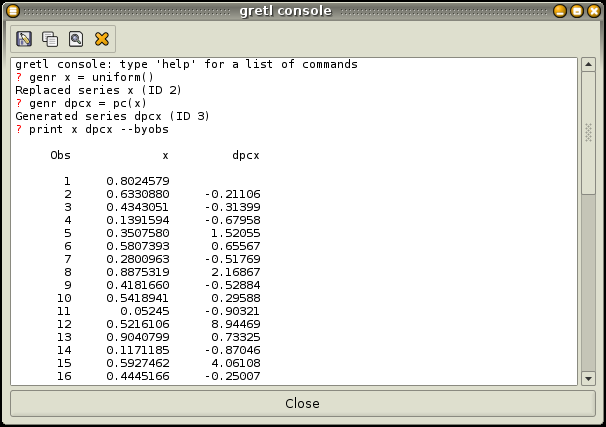
\includegraphics[scale=0.5]{figures/func_check}
  \caption{Output of function check}
  \label{fig:func_check}
\end{figure}

Now run your function. You may want to make sure it works properly by
running a few tests. For example, you may open the console and type

\begin{code}
genr x = uniform()
genr dpcx = pc(x)
print x dpcx --byobs
\end{code}

You should see something similar to figure \ref{fig:func_check}. The
function seems to work ok.  Once your function is debugged, you
may proceed to the next stage.

\subsection{Create a package}

We first present the mechanism for creating a function package via
\app{gretl}'s graphical interface. This can also be done via the
command line, which offers some additional functionality for package
authors; an explanation is given later in this section.

Start the GUI program and take a look at the ``File, Function files'' menu.
This menu contains four items: ``On local machine'', ``On server'', ``Edit
package'', ``New package''.

Select ``New package''.  (This will produce an error message unless at
least one user-defined function is currently loaded in memory --- see
the previous point.)  In the first dialog you get to select:

\begin{itemize}
\item A public function to package.
\item Zero or more ``private'' helper functions.
\end{itemize}

Public functions are directly available to users; private functions are
part of the ``behind the scenes'' mechanism in a function package.

\begin{figure}[htbp]
  \centering
  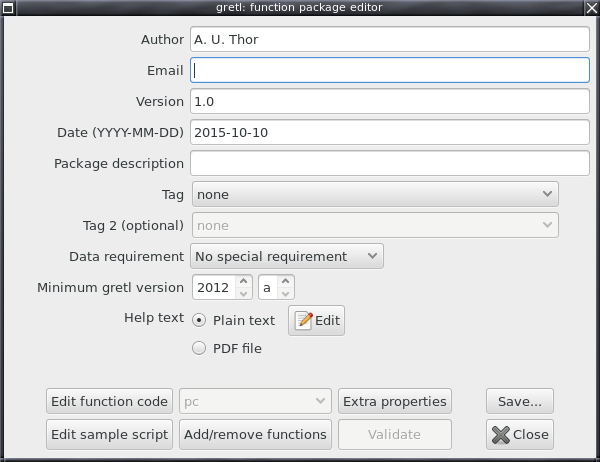
\includegraphics[scale=0.5]{figures/package_editor}
  \caption{The package editor window}
  \label{fig:package_editor}
\end{figure}

On clicking ``OK'' a second dialog should appear (see
Figure~\ref{fig:package_editor}), where you get to enter the package
information (author, version, date, and a short description).  You can
also enter help text for the public interface.  You have a further
chance to edit the code of the function(s) to be packaged, by clicking
on ``Edit function code''.  (If the package contains more than one
function, a drop-down selector will be shown.)  And you get to add a
sample script that exercises your package.  This will be helpful for
potential users, and also for testing.  A sample script is required if
you want to upload the package to the gretl server (for which a
check-box is supplied).

You won't need it right now, but the button labeled ``Save as script''
allows you to ``reverse engineer'' a function package, writing out a
script that contains all the relevant function definitions.

Clicking ``Save'' in this dialog leads you to a File Save dialog.  All
being well, this should be pointing towards a directory named
\texttt{functions}, either under the \app{gretl} system directory (if
you have write permission on that) or the \app{gretl} user directory.
This is the recommended place to save function package files, since
that is where the program will look in the special routine for opening
such files (see below).

Needless to say, the menu command ``File, Function files, Edit package''
allows you to make changes to a local function package.

\vspace{6pt}

A word on the file you just saved.  By default, it will have a
\texttt{.gfn} extension.  This is a ``function package'' file: unlike
an ordinary \app{gretl} script file, it is an XML file containing both
the function code and the extra information entered in the packager.
Hackers might wish to write such a file from scratch rather than using
the GUI packager, but most people are likely to find it awkward.  Note
that XML-special characters in the function code have to be escaped,
e.g.\ \texttt{\&} must be represented as \texttt{\&amp;}.  Also, some
elements of the function syntax differ from the standard script
representation: the parameters and return values (if any) are
represented in XML.  Basically, the function is pre-parsed, and ready
for fast loading using \textsf{libxml}.

\vspace{6pt}

\subsection{Load a package}

Why package functions in this way?  To see what's on offer so far, try
the next phase of the walk-through.

Close gretl, then re-open it.  Now go to ``File, Function files, On
local machine''. If the previous stage above has gone OK, you should
see the file you packaged and saved, with its short description.  If
you click on ``Info'' you get a window with all the information gretl
has gleaned from the function package.  If you click on the ``View
code'' icon in the toolbar of this new window, you get a script view
window showing the actual function code. Now, back to the ``Function
packages'' window, if you click on the package's name, the relevant
functions are loaded into \app{gretl}'s workspace, ready to be called
by clicking on the ``Call'' button.

After loading the function(s) from the package, open the GUI console.
Try typing \texttt{help foo}, replacing \texttt{foo} with the name of
the public interface from the loaded function package: if any help text
was provided for the function, it should be presented.

In a similar way, you can browse and load the function packages
available on the \app{gretl} server, by selecting ``File, Function
files, On server''.

Once your package is installed on your local machine, you can use the
function it contains via the graphical interface as described above,
or by using the CLI, namely in a script or through the console. In the
latter case, you load the function via the \texttt{include} command,
specifying the package file as the argument, complete with the
\texttt{.gfn} extension.

\begin{figure}[htbp]
  \centering
  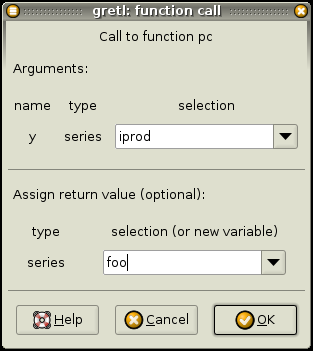
\includegraphics[scale=0.5]{figures/function_call}
  \caption{Using your package}
  \label{fig:function_call}
\end{figure}

To continue with our example, load the file \texttt{np.gdt} (supplied
with \app{gretl} among the sample datasets). Suppose you want to
compute the rate of change for the variable \texttt{iprod} via your
new function and store the result in a series named \texttt{foo}.

Go to ``File, Function files, On local machine''.  You will be shown a
list of the installed packages, including the one you have just
created. If you select it and click on ``Execute'' (or double-click on
the name of the function package), a window similar to the one shown
in figure \ref{fig:function_call} will appear.  Notice that the
description string ``Series to process'', supplied with the function
definition, appears to the left of the top series chooser.

Click ``Ok'' and the series \texttt{foo} will be generated (see figure
\ref{fig:iprod_pc}).  You may have to go to ``Data, Refresh data'' in
order to have your new variable show up in the main window variable
list (or just press the ``r'' key).

\begin{figure}[htbp]
  \centering
  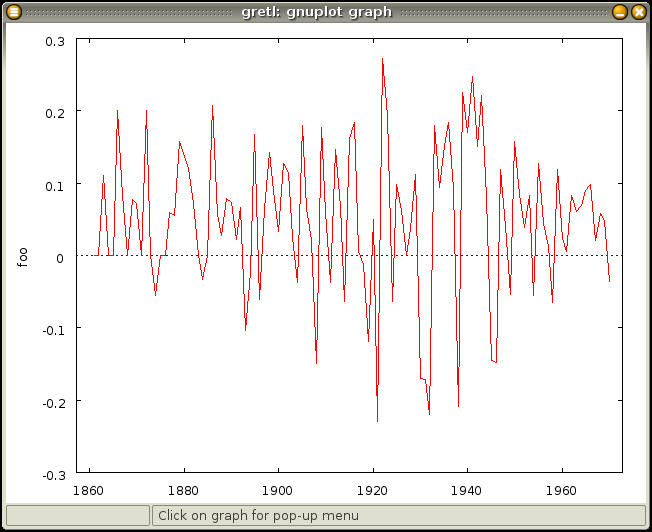
\includegraphics[scale=0.5]{figures/iprod_pc}
  \caption{Percent change in industrial production}
  \label{fig:iprod_pc}
\end{figure}

Alternatively, the same could have been accomplished by the script
\begin{code}
include pc.gfn
open np
foo = pc(iprod)
\end{code}

\subsection{Creating a package via the command line}

The mechanism described above, for creating function packages using
the GUI, is likely to be convenient for small to medium-sized packages
but may be too cumbersome for ambitious packages that include a large
hierarchy of private functions. To facilitate the building of such
packages \app{gretl} offers the \texttt{makepkg} command.

To use \texttt{makepkg} you create three files: a driver script that
loads all the functions you want to package and invokes
\texttt{makepkg}; a small, plain-text specification file that contains
the required package details (author, version, etc.); and (in the
simplest case) a plain text help file.  You run the driver script and
\app{gretl} writes the package (\texttt{.gfn}) file.

We first illustrate with a simple notional package. We have a gretl
script file named \texttt{foo.inp} that contains a function,
\texttt{foo}, that we want to package. Our driver script would then
look like this
%
\begin{code}
include foo.inp
makepkg foo.gfn
\end{code}
%
Note that the \texttt{makepkg} command takes one argument, the name of
the package file to be created. The package \emph{specification file}
should have the same basename but the extension \texttt{.spec}. In
this case \app{gretl} will therefore look for \texttt{foo.spec}. It
should look something like this:
%
\begin{code}
# foo.spec
author = A. U. Thor
version = 1.0
date = 2011-02-01
description = Does something with time series
public = foo 
help = foohelp.txt
sample-script = example.inp
min-version = 1.9.3
data-requirement = needs-time-series-data
\end{code}

As you can see, the format of each line in this file is \texttt{key =
  value}, with two qualifications: blank lines are permitted (and
ignored, as are comment lines that start with \verb|#|). 

All the fields included in the above example are required, with the
exception of \texttt{data-requirement}, though the order in which they
appear is immaterial. Here's a run-down of the basic fields:

\begin{itemize}
\item \texttt{author}: the name(s) of the author(s). Accented or other
  non-ASCII characters should be given as UTF-8.
\item \texttt{version}: the version number of the package, which should
  be limited to two integers separated by a period.
\item \texttt{date}: the release date of the current verson of the
  package, in ISO 8601 format: YYYY-MM-DD.
\item \texttt{description}: a brief description of the functionality
  offered by the package. This will be displayed in the GUI function
  packages window so it should be just one short line.
\item \texttt{public}: the listing of public functions.
\item \texttt{help}: the name of a plain text (UTF-8) file containing
  help; all packages must provide help.
\item \texttt{sample-script}: the name of a sample script that
 illustrates use of the package; all packages must supply a
 sample script.
\item \texttt{min-version}: the minimum version of gretl required
 for the package to work correctly. If you're unsure about this,
 the conservative thing is to give the current \app{gretl} version.
\end{itemize}

The \texttt{public} field indicates which function or functions are to
be made directly available to users (as opposed to private ``helper''
functions).  In the example above there is just one public
function. Note that any functions in memory when \texttt{makepkg} is
invoked, other than those designated as public, are assumed to be
private functions that should also be included in the package. That
is, the list of private functions (if any) is implicit.

The \texttt{data-requirement} field should be specified if the package
requires time-series or panel data, or alternatively if no dataset is
required.  If the \texttt{data-requirement} field is omitted, the
assumption is that the package needs a dataset in place, but it
doesn't matter what kind; if the packaged functions do not use any
series or lists this requirement can be explicitly relaxed.  Valid
values for this field are:

\begin{center}
\begin{tabular}{ll}
\texttt{needs-time-series-data} & (any time-series data OK) \\ 
\texttt{needs-qm-data} & (must be quarterly or monthly) \\ 
\texttt{needs-panel-data} & (must be a panel) \\
\texttt{no-data-ok} & (no dataset is needed) \\
\end{tabular}
\end{center}

For a more complex example, let's look at the \app{gig}
(GARCH-in-gretl) package.  The driver script for building \app{gig}
looks something like this:
%
\begin{code}
set echo off
set messages off
include gig_mle.inp
include gig_setup.inp
include gig_estimate.inp
include gig_printout.inp
include gig_plot.inp
makepkg gig.gfn
\end{code}

In this case the functions to be packaged (of which there are many)
are distributed across several script files, each of which is the
target of an \texttt{include} command.  The \texttt{set} commands at
the top are included to cut down on the verbosity of the output.

The content of \texttt{gig.spec} is as follows:
%
\begin{code}
author = Riccardo "Jack" Lucchetti and Stefano Balietti
version = 2.0
date = 2010-12-21
description = An assortment of univariate GARCH models
public = GUI_gig \
    gig_setup gig_set_dist gig_set_pq gig_set_vQR \
    gig_print gig_estimate \
    gig_plot gig_dplot \
    gig_bundle_print GUI_gig_plot

gui-main = GUI_gig
bundle-print = gig_bundle_print
bundle-plot = GUI_gig_plot
help = gig.pdf
sample-script = examples/example1.inp
min-version = 1.9.3
data-requirement = needs-time-series-data
\end{code}

Note that backslash continuation can be used for the elements of the
\texttt{public} function listing.

In addition to the fields shown in the simple example above,
\texttt{gig.spec} includes three optional fields: \texttt{gui-main},
\texttt{bundle-print} and \texttt{bundle-plot}. These keywords are
used to designate certain functions as playing a special role in the
\app{gretl} graphical interface. A function picked out in this way
must be in the \texttt{public} list and must satisfy certain
further requirements.  
%
\begin{itemize}
\item \texttt{gui-main}: this specifies a function as the one which
  will be presented automatically to GUI users (instead of users'
  being faced with a choice of interfaces). This makes sense only for
  packages that have multiple public functions. In addition, the
  \texttt{gui-main} function must return a \texttt{bundle} (see
  section~\ref{sec:Bundles}).
\item \texttt{bundle-print}: this picks out a function that should be
  used to print the contents of a bundle returned by the
  \texttt{gui-main} function. It must take a pointer-to-bundle as its
  first argument. The second argument, if present, should be an
  \texttt{int} switch, with two or more valid values, that controls the
  printing in some way. Any further arguments must have default values
  specified so that they can be omitted.
\item \texttt{bundle-plot}: selects a function for the role of
  producing a plot or graph based on the contents of a returned
  bundle. The requirements on this function are as for 
  \texttt{bundle-print}.
\end{itemize}

The ``GUI special'' tags support a user-friendly mode of operation.
On a successful call to \texttt{gui-main}, \app{gretl} opens a 
window displaying the contents of the returned bundle (formatted
via \texttt{bundle-print}). Menus in this window give the user the
option of saving the entire bundle (in which case it's represented
as an icon in the ``icon view'' window) or of extracting specific
elements from the bundle (series or matrices, for example). 

If the package has a \texttt{bundle-plot} function, the bundle window
also has a \textsf{Graph} menu. In \app{gig}, for example, the
\texttt{bundle-plot} function has this signature:
%
\begin{code}
function void GUI_gig_plot(bundle *model, int ptype[0:1:0] \
                           "Plot type" {"Time series", "Density"})
\end{code}

The \texttt{ptype} switch is used to choose between a time-series plot
of the residual and its conditional variance, and a kernel density
plot of the innovation against the theoretical distribution it is
supposed to follow. The use of the value-labels \texttt{Time series}
and \texttt{Density} means that the \textsf{Graph} menu will display
these two choices.

One other feature of the \app{gig} spec file is noteworthy: the
\texttt{help} field specifies \texttt{gig.pdf}, documentation in PDF
format. Unlike plain-text help, this cannot be rolled into the
\texttt{gfn} (XML) file produced by the \texttt{makepkg} command;
rather, both \texttt{gig.gfn} and \texttt{gig.pdf} are packaged into a
zip archive for distribution. This represents a form of package
which is new in \app{gretl} 1.9.4. More details will be made
available before long. 

\section{Memo: updating old-style functions}
\label{sec:old-func}

As mentioned at the start of this chapter, different rules were in
force for defining functions prior to \app{gretl} 1.8.4. While the old
syntax is still supported to date, this may not always be the
case. But it is straightforward to convert a function to the new
style. The only thing that must be changed for compatibility with the
new syntax is the declaration of the function's return
type. Previously this was placed inline in the \texttt{return}
statement, whereas now it is placed right after the \texttt{function}
keyword. For example:
%
\begin{code}
# old style
function triple (series x)
  y = 3*x
  return series y # note the "series" here
end function

# new style
function series triple (series x)
  y = 3*x
  return y
end function
\end{code}

Note also that the role of the \texttt{return} statement has changed
(and its use has become more flexible):

\begin{itemize}
\item The \texttt{return} statement now causes the function to return
  directly, and you can have more than one such statement, wrapped in
  conditionals. Before there could only be one \texttt{return}
  statement, and its role was just to specify the type available for
  assignment by the caller.
\item The final element in the \texttt{return} statement can now be an
  expression that evaluates to a value of the advertised return type;
  before, it had to be the name of a pre-defined variable.
\end{itemize}


%%% Local Variables: 
%%% mode: latex
%%% TeX-master: "gretl-guide"
%%% End: 


\chapter{Oggetti persistenti}
\label{persist}

%%% Work in progress, not really ready for translation yet.

%FIXME This chapter needs to deal with saving models too.

\section{Liste definite dall'utente}
\label{named-lists}

Molti comandi di \app{gretl} richiedono come argomenti una o pi� liste di
variabili. Per semplificare la loro gestione negli script di comandi, in
particolare nelle funzioni definite dall'utente, \app{gretl} offre la
possibilit� di creare \textit{liste definite dall'utente}.  

\subsection{Creazione e modifica di una lista}

Per creare una lista occorre usare il comando \texttt{list}, seguito dal nome
della lista, un segno di uguale, e, in alternativa, \texttt{null} (per creare
una lista vuota) o il nome di una o pi� variabili da inserire nella lista. Ad
esempio:
%
\begin{code}
list xlist = 1 2 3 4
list reglist = income price 
list empty_list = null
\end{code}

Il nome della lista deve iniziare con una lettera e deve essere composto
interamente da lettere, numeri o il carattere trattino basso (non da spazi). La
lunghezza massima del nome � di 15 caratteri. Quando si aggiungono variabili a
una lista � possibile riferirsi a essa per nome o per numero identificativo.

Una volta creata, una lista viene ``ricordata'' per l'intera durata della
sessione di \app{gretl} e pu� essere usata nel contesto di qualsiasi comando
\app{gretl} che accetta liste di variabili. Un semplice esempio � la
specificazione di una lista di regressori:
%
\begin{code}
list xlist = x1 x2 x3 x4
ols y 0 xlist
\end{code}

Le liste possono essere modificate in due modi. Per \textit{ridefinire} una
lista si usa la stessa sintassi usata per crearla. Ad esempio
%
\begin{code}
list xlist = 1 2 3
list xlist = 4 5 6
\end{code}

Dopo il secondo comando, \texttt{xlist} contiene solo le variabili 4,
5 e 6.

Per \textit{accodare} o \textit{premettere} variabili a una lista esistente,
� possibile usare il nome di una lista all'interno del comando di definizione
della lista stessa. Ad esempio, � possibile scrivere
%
\begin{code}
list xlist = xlist 5 6 7
list xlist = 9 10 xlist 11 12
\end{code}

\subsection{Interrogazione delle liste}

� possibile determinare se una variabile sconosciuta rappresenta una lista
usando la funzione \texttt{islist()}.
%
\begin{code}
series xl1 = log(x1)
series xl2 = log(x2)
list xlogs = xl1 xl2
genr is1 = islist(xlogs)
genr is2 = islist(xl1)
\end{code}

Il primo comando \texttt{genr} assegner� il valore 1 a \texttt{is1} visto che
\texttt{xlogs} in effetti � una lista. Il secondo comando genr assegner� il
valore 0 a \texttt{is2}, visto che \texttt{xl1} � una serie di dati, non una
lista.

� anche possibile determinare il numero di elementi che compongono una lista
usando la funzione \texttt{nelem()}.
%
\begin{code}
list xlist = 1 2 3
genr nl = nelem(xlist)
\end{code}

Lo scalare \texttt{nl} avr� un valore di 3, visto che
\texttt{xlist} contiene 3 membri.

� possibile mostrare i membri di una lista come illustrato in questa sessione
interattiva:
%
\begin{code}
? list xlist = x1 x2 x3
 # list xlist = x1 x2 x3
Added list 'xlist'
? list xlist print
 # list xlist = x1 x2 x3
\end{code}
%
Si noti che \texttt{print xlist} produrr� un effetto diverso, ossia mostrer� i
valori di tutte le variabili contenute in \texttt{xlist} (come ci si pu�
aspettare).

\subsection{Liste di variabili trasformate}

Data una lista di variabili, � possibile generare liste che contengono
trasformazioni di queste variabili usando una forma speciale dei comandi
\texttt{logs}, \texttt{lags}, \texttt{diff}, \texttt{ldiff},
\texttt{sdiff} o \texttt{square}. In pratica basta far seguire questi comandi
dal nome della lista tra parentesi. Ad esempio:
%
\begin{code}
list xlist = x1 x2 x3
list lxlist = logs(xlist)
list difflist = diff(xlist)
\end{code}

Quando si genera una lista di \textit{ritardi} in questo modo, � possibile
specificare il massimo ordine di ritardi, inserendolo per primo tra parentesi e
separandolo dal nome della lista con una virgola. Ad esempio
%
\begin{code}
list xlist = x1 x2 x3
list laglist = lags(2, xlist)
\end{code}
%
oppure
%
\begin{code}
scalar order = 4
list laglist = lags(order, xlist)
\end{code}

Questi comandi riempiranno \texttt{laglist} col numero specificato di ritardi
delle variabili presenti in \texttt{xlist}. Come avviene per il normale comando
\texttt{lags} � possibile omettere l'ordine, che sar� cos� determinato
automaticamente a seconda della frequenza dei dati. Un altro modo speciale di
utilizzare questi comandi consiste nell'indicare tra parentesi il nome di una
singola variabile al posto di quello di una lista, come in
%
\begin{code}
series lx = log(x)
list laglist = lags(4, lx)
\end{code}

Si noti che la sintassi normale per questi comandi, ad esempio \texttt{logs},
� semplicemente
%
\begin{code}
logs x1 x2 x3
\end{code}
%
Se \texttt{xlist} � una lista, � anche possibile scrivere
%
\begin{code}
logs xlist
\end{code}
%
ma questo comando non salver� i logaritmi in una lista; per avere questo
risultato occorre usare la sintassi
%
\begin{code}
list loglist = logs(xlist)
\end{code}


\subsection{Controllo dei valori mancanti}

\app{Gretl} offre varie funzioni per riconoscere e gestire i valori mancanti (si
veda la \GCR{} per i dettagli). In questa sede � utile ricordare che la funzione
\texttt{ok()} pu� essere usata con un argomento lista. Ad esempio:
%
\begin{code}
list xlist = x1 x2 x3
series xok = ok(xlist)
\end{code}
%
Dopo questi comandi, la serie \texttt{xok} avr� valore 1 per le osservazioni in
cui nessuna variabile tra \texttt{x1}, \texttt{x2}, e
\texttt{x3} ha un valore mancante, e valore 0 per le osservazioni che non
soddisfano questa condizione.


\section{Stringhe definite dall'utente}
\label{named-strings}

In alcuni casi pu� essere utile salvare una stringa (ossia una sequenza di
caratteri) sotto forma di variabile che possa essere riutilizzata.
\app{Gretl} offre questa funzionalit� a partire dalla versione 1.6.0.

Per \textit{definire} una variabile stringa � possibile usare uno dei comandi
seguenti: \texttt{string} o \texttt{sprintf}.  Il comando \texttt{string}
� il pi� semplice: basta scrivere, ad esempio
%
\begin{code}
string pippo = "Qualcosa da ricordare"
\end{code}
%
Il primo campo dopo \texttt{string} � il nome della variabile che verr� creata,
quindi segue il segno di uguale, infine la stringa da salvare, racchiusa tra
virgolette doppie. Quest'ultima pu� anche essere indicata come sequenza di
sotto-stringhe, come in questo esempio:
%
\begin{code}
string pezzi = "Primo " "e" " secondo"
\end{code}
%
Il comando \texttt{sprintf} � pi� flessibile. Funziona esattamente come
\texttt{printf}, tranne per il fatto che la stringa ``di formato'' deve
essere preceduta dal nome di una variabile stringa. Ad esempio,
%
\begin{code}
scalar x = 8
sprintf pippo "var%d", x
\end{code}
%
Per \textit{recuperare il valore} di una variabile stringa, basta usare il nome
della variabile preceduto dal carattere ``at'', \verb|@|.  In un comando
\app{gretl}, una sequenza di caratteri che segue il simbolo \verb|@| viene
trattata come il nome di una variabile stringa e il valore della variabile viene
sostituito sulla riga di comando, come avviene in questo esempio di sessione
interattiva:
%
\begin{code}
? scalar x = 8
 scalar x = 8
Generato lo scalare x (ID 2) = 8
? sprintf pippo "var%d", x
Salvata la stringa 'pippo'
? print "@foo"
var8
\end{code}

\subsection{Stringhe predefinite}

Oltre alle stringhe definite dall'utente, \app{gretl} contiene alcune variabili
stringa predefinite che possono essere utili per chi scrive funzioni che
includono comandi shell. Le stringhe predefinite sono mostrate nella
Tabella~\ref{tab-strings}.

\begin{table}[htbp]
\centering
\begin{tabular}{ll}
  \verb|@gretldir| & La directory di installazione di \app{gretl} \\
  \verb|@userdir| & La directory utente di \app{gretl} \\
  \verb|@gnuplot| & Percorso, o nome, dell'eseguibile \app{gnuplot} \\
  \verb|@tramo| & Percorso, o nome, dell'eseguibile \app{tramo} \\
  \verb|@x12a| & Percorso, o nome, dell'eseguibile \app{x-12-arima} \\
  \verb|@tramodir| & Directory dei dati di \app{tramo} \\
  \verb|@x12adir| & Directory dei dati di \app{x-12-arima} \\
\end{tabular}
\caption{Variabili stringa predefinite}
\label{tab-strings}
\end{table}

%%% Local Variables: 
%%% mode: latex
%%% TeX-master: "gretl-guide"
%%% End: 


\chapter{Matrix manipulation}
\label{chap:matrices}

\section{Introduction}
\label{matrix-intro}

Since version 1.5.1, gretl has offered the facility of creating and
manipulating user-defined matrices.  There are a few changes in this
respect in version 1.6.1.

\section{Creating matrices}
\label{matrix-create}

Matrices can be created using any of these methods:

\begin{enumerate}
\item By direct specification of the scalar values that compose the
  matrix, in numerical form, by reference to pre-existing
  scalar variables, or using computed values.
\item By providing a list of data series.
\item By providing a \textit{named list} of series.
\item Using a formula of the same general type that is used
  with the \texttt{genr} command, whereby a new matrix is defined
  in terms of existing matrices and/or scalars, or via some
  special functions.
\end{enumerate}

To specify a matrix \textit{directly in terms of scalars}, the syntax
is, for example:

\begin{code}
matrix A = { 1, 2, 3 ; 4, 5, 6 }
\end{code}

The matrix is defined by rows; the elements on each row are separated
by commas and the rows are separated by semi-colons.  The whole
expression must be wrapped in braces.  Spaces within the braces are
not significant.  The above expression defines a $2\times3$ matrix.
Each element should be a numerical value, the name of a scalar
variable, or an expression that evaluates to a scalar.  Directly after
the closing brace you can append a single quote (\texttt{'}) to obtain
the transpose.

To specify a matrix \textit{in terms of data series} the syntax is,
for example,
%
\begin{code}
matrix A = { x1, x2, x3 }
\end{code}
%
where the names of the variables are separated by commas.  Besides
names of existing variables, you can use expressions that evaluate to
a series.  For example, given a series \texttt{x} you could do
%
\begin{code}
matrix A = { x, x^2 }
\end{code}
%
Each variable occupies a column (and there can only be one variable
per column).  You cannot use the semi-colon as a row separator in this
case: if you want the series arranged in rows, append the transpose
symbol.  The range of data values included in the matrix depends on
the current setting of the sample range.

Please note: while gretl's built-in statistical functions are
capable of handling missing values, the matrix arithmetic functions
are not.  \emph{When you build a matrix from series that include missing
values, observations for which at least one series has a missing value
are skipped}.  

Instead of giving an explicit list of variables, you may instead
provide the \textit{name of a saved list} (see
Chapter~\ref{chap-persist}), as in
%
\begin{code}
list xlist = x1 x2 x3
matrix A = { xlist }
\end{code}
%
When you provide a named list, the data series are by default placed
in columns, as is natural in an econometric context: if you want them
in rows, append the transpose symbol.

As a special case of constructing a matrix from a list of variables,
you can say
%
\begin{code}
matrix A = { dataset }
\end{code}
%
This builds a matrix using all the series in the current dataset,
apart from the constant (variable 0).  When this dummy list is used, it
must be the sole element in the matrix definition \texttt{\{...\}}.  You
can, however, create a matrix that includes the constant along with
all other variables using column-wise concatenation (see below), as in
%
\begin{code}
matrix A = {const}~{dataset}
\end{code}
%

You can create new matrices, or replace existing matrices, by means of
various transformations just as with scalars and data series.  The
relevant mechanisms are discussed in the next several sections.

\tip{Names of matrices must satisfy the same requirements as names of
  gretl variables in general: the name can be no longer than 15
  characters, must start with a letter, and must be composed of
  nothing but letters, numbers and the underscore character.}

\section{Matrix operators}
\label{matrix-op}

The following binary operators are available for matrices:

\begin{center}
\begin{tabular}{ll}
\texttt{+}  & addition \\
\texttt{-}  & subtraction \\
\texttt{*}  & ordinary matrix multiplication \\
\texttt{'}  & pre-multiplication by transpose \\
\texttt{/}  & matrix ``division'' (see below) \\
\texttt{.*} & element-wise multiplication \\
\texttt{./} & element-wise division \\
\verb+.^+   & element-wise exponentiation \\
\verb+~+    & column-wise concatenation \\
\verb+|+    & row-wise concatenation \\
\texttt{**} & Kronecker product \\
\texttt{=}  & test for equality 
\end{tabular}
\end{center}

Here are explanations of the less obvious cases. 

For matrix addition and subtraction, in general the two matrices have
to be of the same dimensions but an exception to this rule is granted
if one of the operands is a $1\times 1$ matrix or scalar.  The scalar
is implicitly promoted to the status of a matrix of the correct
dimensions, all of whose elements are equal to the given scalar value.
For example, if $A$ is an $m \times n$ matrix and $k$ a scalar, then
the commands
%
\begin{code}
matrix C = A + k
matrix D = A - k
\end{code}
%
both produce $m \times n$ matrices, with elements $c_{ij} = 
a_{ij} + k$ and $d_{ij} = a_{ij} - k$ respectively.

By ``pre-multiplication by transpose'' we mean, for example, that 
%
\begin{code}
matrix C = X'Y
\end{code}
%
produces the product of $X$-transpose and $Y$.  In effect, 
the expression \texttt{X'Y} is shorthand for \texttt{X'*Y}
(which is also valid).

In matrix ``division'', $A/B$ is algebraically equivalent to
$B^{-1}A$ (pre-multiplication by the inverse of the ``divisor'').
Therefore the following two expressions are equivalent in principle:
%
\begin{code}
matrix C = A / B
matrix C = inv(B) * A
\end{code}
%
where \texttt{inv()} is the matrix inversion function (see below for
more on matrix functions).  The first form, however, may be more
accurate than the second; the solution is obtained via LU
decomposition, without the explicit calculation of the inverse.

In \textit{element-wise multiplication} if we write
%
\begin{code}
matrix C = A .* B
\end{code}
% 
then the result depends on the dimensions of $A$ and $B$.  Let $A$ be
an $m \times n$ matrix and let $B$ be $p \times q$.  
%
\begin{itemize}
\item If $m=p$ and $n=q$ then $C$ is $m\times n$ with $c_{ij} = a_{ij}
  \times b_{ij}$.  This is known as the \emph{Hadamard product}.
\item Otherwise, if $m=1$ and $n=q$, or $n=1$ and $m=p$, then $C$ is
  $p\times q$ with $c_{ij} = a_k \times b_{ij}$, where $k=j$ if $m=1$
  else $k=i$.
\item Otherwise, if $p=1$ and $n=q$, or $q=1$ and $m=p$, then $C$ is
  $m\times n$ with $c_{ij} = a_{ij} \times b_k$, where $k=j$ if $p=1$
  else $k=i$.
\item If none of the above conditions are satisfied the product is
  undefined and an error is flagged.
\end{itemize}
For example, if $A$ is a row vector with the same number of
columns of $B$, then the columns of $C$ are the columns of $B$
multiplied by the corresponding element of $A$.  Note that this
convention makes it unnecessary, in most cases, to use diagonal
matrices to perform transformations by means of ordinary matrix
multiplication: if $Y = XV$, where $V$ is diagonal, it is
computationally much more convenient to obtain $Y$ via the
instruction
%
\begin{code}
matrix Y = X .* v
\end{code}
%
where \texttt{v} is a row vector containing the diagonal of $V$.

Element-wise division and element-wise exponentiation work in a manner
exactly analogous to element-wise multiplication: simply replace
$\times$ by $\div$, or the exponentation operation, in the account
given for multiplication.

In \textit{column-wise concatenation} of an $m\times n$ matrix $A$ and
an $m\times p$ matrix $B$, the result is an $m\times (n+p)$ matrix.
That is,
%
\begin{code}
matrix C = A ~ B
\end{code}
% 
produces $C = \left[ \begin{array}{cc} A & B \end{array} \right]$.

\textit{Row-wise concatenation} of an $m\times n$ matrix $A$ and
an $p\times n$ matrix $B$ produces an $(m+p) \times n$ matrix.
That is,
%
\begin{code}
matrix C = A | B
\end{code}
% 
produces $C = \left[ \begin{array}{cc} A \\ B \end{array} \right]$.

\section{Matrix--scalar operators}
\label{matrix-scalar-op}

For matrix $A$ and scalar $k$, the operators shown in
Table~\ref{tab:matrix-scalar-ops} are available.  (Addition and
subtraction were discussed in section~\ref{matrix-op} but we include
them in the table for completeness.)  In addition, for square $A$ and
integer $k \geq 0$, \verb|B = A^k| produces a matrix $B$ which is $A$
raised to the power $k$.  (Note that the operator \texttt{**} cannot
be used in place of \verb|^| for this purpose because in a matrix
context it is reserved for the Kronecker product.)

\begin{table}[htbp]
\centering
\begin{tabular}{ll}
\textit{Expression} & \textit{Effect} \\[4pt]
\texttt{matrix B = A * k} & $b_{ij} = k a_{ij}$ \\
\texttt{matrix B = A / k} & $b_{ij} = a_{ij} / k$ \\
\texttt{matrix B = k / A} & $b_{ij} = k / a_{ij}$ \\
\texttt{matrix B = A + k} & $b_{ij} = a_{ij} + k$ \\
\texttt{matrix B = A - k} & $b_{ij} = a_{ij} - k$ \\
\texttt{matrix B = k - A} & $b_{ij} = k - a_{ij}$ \\
\texttt{matrix B = A \% k} & $b_{ij} = a_{ij} \mbox{ modulo } k$ \\
\end{tabular}
\caption{Matrix--scalar operators}
\label{tab:matrix-scalar-ops}
\end{table}


\section{Matrix functions}
\label{matrix-func}

\begin{table}[htbp]
\centering
\textbf{Creation}
\hrulefill

\begin{tabular}{p{0.1\textwidth}p{0.1\textwidth}p{0.1\textwidth}p{0.1\textwidth}p{0.1\textwidth}p{0.1\textwidth}}
\texttt{I}         &
\texttt{mnormal}   &
\texttt{muniform}  &
\texttt{ones}      &
\texttt{seq}       &
\texttt{zeros}     
\end{tabular}      

\textbf{Shape/size}
\hrulefill

\begin{tabular}{p{0.1\textwidth}p{0.1\textwidth}p{0.1\textwidth}p{0.1\textwidth}p{0.1\textwidth}p{0.1\textwidth}}
\texttt{cols}      &
\texttt{diag}      &
\texttt{dsort}     &
\texttt{mlag}      &
\texttt{mshape}    &
\texttt{rows}      \\
\texttt{sort}      &
\texttt{transp}    &
\texttt{unvech}    &
\texttt{vec}       &
\texttt{vech}      
\end{tabular}      

\textbf{Element by element}
\hrulefill

\begin{tabular}{p{0.1\textwidth}p{0.1\textwidth}p{0.1\textwidth}p{0.1\textwidth}p{0.1\textwidth}p{0.1\textwidth}}
\texttt{abs}       &
\texttt{atan}      &
\texttt{cnorm}     &
\texttt{cos}       &
\texttt{dnorm}     &
\texttt{exp}       \\
\texttt{gamma}     &
\texttt{int}       &
\texttt{lngamma}   &
\texttt{log}       &
\texttt{qnorm}     &
\texttt{sin}       \\
\texttt{sqrt}      &
\texttt{tan}       
\end{tabular}      

\textbf{Matrix algebra}
\hrulefill

\begin{tabular}{p{0.1\textwidth}p{0.1\textwidth}p{0.1\textwidth}p{0.1\textwidth}p{0.1\textwidth}p{0.1\textwidth}}
\texttt{cholesky}  &
\texttt{det}       &
\texttt{eigengen}  &
\texttt{eigensym}  &
\texttt{infnorm}   &
\texttt{inv}       \\
\texttt{ldet}      &
\texttt{mexp}      &
\texttt{nullspace} &
\texttt{onenorm}   &
\texttt{qform}     &
\texttt{qrdecomp}  \\
\texttt{rank}      &
\texttt{rcond}     &
\texttt{svd}       &
\texttt{tr}        &
\end{tabular}      

\textbf{Statistical}
\hrulefill

\begin{tabular}{p{0.1\textwidth}p{0.1\textwidth}p{0.1\textwidth}p{0.1\textwidth}p{0.1\textwidth}p{0.1\textwidth}}
\texttt{cdemean}   &
\texttt{imaxc}     &
\texttt{imaxr}     &
\texttt{iminc}     &
\texttt{iminr}     &
\texttt{mcorr}     \\
\texttt{mcov}      &
\texttt{maxc}      &   
\texttt{maxr}      &
\texttt{meanc}     &
\texttt{meanr}     &
\texttt{minc}      \\   
\texttt{minr}      &
\texttt{princomp}  &
\texttt{sumc}      &
\texttt{sumr}      &
\texttt{values}    &
\end{tabular}      
\caption{Table of matrix functions by category}
\label{tab:matrix_funcs_cat}
\end{table}

Table \ref{tab:matrix_funcs_cat} lists the matrix function that
\app{gretl} provides (an alphabetized version of the table is
provided at the end of this chapter as Table~\ref{tab:matrix_funcs}).
The following functions are available for \textit{element-by-element
  transformations} of matrices: \texttt{log}, \texttt{exp},
\texttt{sin}, \texttt{cos}, \texttt{tan}, \texttt{atan}, \texttt{int},
\texttt{abs}, \texttt{sqrt}, \texttt{dnorm}, \texttt{cnorm},
\texttt{qnorm}, \texttt{gamma} and \texttt{lngamma}.  These functions
have the effects documented in relation to the \texttt{genr} command.
For example, if a matrix \texttt{A} is already defined, then
%
\begin{code}
matrix B = sqrt(A)
\end{code}
%
generates a matrix such that $b_{ij} = \sqrt{a_{ij}}$.  All of these
functions require a single matrix as argument, or an expression which
evaluates to a single matrix.

Note that to find the ``matrix square root'' you need the
\texttt{cholesky()} function (see below); moreover, the \texttt{exp()}
function computes the exponential element by element, and therefore
does \emph{not} return the matrix exponential unless the matrix is
diagonal --- to get the matrix exponential, use \texttt{mexp()}.
  
The functions \texttt{sort()}, \texttt{dsort()} and \texttt{values()}
are available for matrices as well as data series.  In the matrix case
the argument to these functions must be a vector ($p \times 1$ or
$1\times p$).  For \texttt{sort} and \texttt{dsort} the return value
is a vector containing the elements of the input vector sorted in
ascending (\texttt{sort}) or descending (\texttt{dsort}) order of
magnitude.  For \texttt{values} the return is a vector containing the
distinct values in the input vector, sorted in ascending order.

Several matrix-specific functions are available.  These functions fall
into five categories:
%
\begin{enumerate}
\item Those taking a single matrix as argument and returning a scalar.
\item Those taking a single matrix as argument (plus in some cases an
  additional parameter) and returning a matrix.
\item Those taking one or two dimensions as arguments and
  returning a matrix.
\item Those taking two matrices as arguments and returning a matrix.
\item Those taking one or two matrices as arguments and returning one
  or two matrices.
\end{enumerate}
%
These sets of functions are discussed in turn below.

\subsection{Matrix to scalar functions}
\label{matrix-to-scalar}

The functions which take a single matrix as argument and return a
scalar are:

\begin{center}
\begin{tabular}{ll}
\texttt{rows()} & number of rows \\
\texttt{cols()} & number of columns \\
\texttt{rank()} & rank \\
\texttt{det()} & determinant \\
\texttt{ldet()} & log-determinant \\
\texttt{tr()} & trace \\
\texttt{onenorm()} & 1-norm \\
\texttt{infnorm()} & infinity-norm \\
\texttt{rcond()} & reciprocal condition number
\end{tabular}
\end{center}

The single matrix argument to these functions may be given as the name
of an existing matrix or as an expression that evaluates to a single
matrix.  Note that the functions \texttt{det}, \texttt{ldet} and
\texttt{tr} require a square matrix as input.  The \texttt{rank()}
function is computed via the QR decomposition.

The functions \texttt{onenorm} and \texttt{infnorm} function return,
respectively, the 1-norm and the infinity-norm of a matrix.  The
former is the maximum across the columns of the matrix of the sums of
the absolute values of the column elements, while the latter is the
maximum across the rows of the matrix of the sums of the absolute
values of the row elements.  The function \texttt{rcond} returns the
reciprocal condition number for a symmetric, positive definite matrix.

\subsection{Matrix to matrix functions}
\label{matrix-to-matrix}

The functions which take a single matrix as argument and return a
matrix are:

\begin{center}
\begin{tabular}{llcll}
\texttt{sumc()}    & sum by column & &
\texttt{sumr()}    & sum by row \\
\texttt{meanc()}   & mean by column & &
\texttt{meanr()}   & mean by row \\
\texttt{mcov()}    & covariance matrix & &
\texttt{mcorr()}   & correlation matrix \\
\texttt{mexp()}    & matrix exponential & &
\texttt{inv()}     & inverse \\
\texttt{cholesky()} & Cholesky decomposition & &
\texttt{diag()}    & extract principal diagonal \\
\texttt{transp()}  & transpose & &
\texttt{cdemean()} & subtract column means \\ 
\texttt{vec()}     & elements as column vector & &
\texttt{vech()}    & vectorize lower triangle \\
\texttt{unvech()}  & undo \texttt{vech} & &
\texttt{mlag()}    & matrix lag or lead \\
\texttt{nullspace()} & right nullspace & &
\texttt{princomp()} & principal components \\
\texttt{maxc}      & column maxima (values) & &
\texttt{maxr}      & row maxima (values) \\
\texttt{imaxc}     & column maxima (indices) & &
\texttt{imaxr}     & row maxima (indices) \\
\texttt{minc}      & column minima (values) & &
\texttt{minr}      & row minima (values) \\
\texttt{iminc}     & column minima (indices) & &
\texttt{iminr}     & row minima (indices) 
\end{tabular}
\end{center}

As with the previous set of functions, the argument may be given as
the name of an existing matrix or as an expression that evaluates to a
single matrix.

For an $m \times n$ matrix $A$, \texttt{sumc(A)} returns a row vector
holding the $n$ column sums, and \texttt{sumr(A)} returns a column
vector with the $m$ row sums.  \texttt{meanc(A)} returns a row vector
with the $n$ column means, and \texttt{meanr(A)} a column vector with
the $m$ row means.

Also for an $m \times n$ matrix $A$, the \texttt{max} and \texttt{min}
family of functions return either an $m \times 1$ matrix (the
\texttt{r} variants, which select the extremum of each row) or a $1
\times n$ matrix (the \texttt{c} variants, which select the column
extrema).  The \texttt{max} vectors contain the values of the row or
column maxima while the \texttt{min} ones hold the row or column
minima.  The variants with an \texttt{i} prefix (e.g.\ \texttt{imaxc})
return not the values but the (1-based) indices of the respective
maxima or minima.

For a $T \times k$ matrix $A$, \texttt{mcov(A)} and \texttt{mcorr(A)}
both return $k \times k$ symmetric matrices, in the first case
containing the variances (on the diagonal) and covariances of the
variables in the columns of $A$, and in the second, containing the
correlations of the variables.

For an $n \times n$ matrix $A$, \texttt{mexp(A)} returns an $n \times
n$ matrix holding the matrix exponential,
\[
e^A = \sum_{k=0}^{\infty} \frac{A^k}{k!} = \frac{I}{0!} + \frac{A}{1!}
 + \frac{A^2}{2!} + \frac{A^3}{3!} + \cdots
\]
(This series is sure to converge.)

The \texttt{cholesky} function computes the Cholesky decomposition $L$
of a symmetric positive definite matrix $A$: $A = LL'$; $L$ is lower
triangular (has zeros above the diagonal).  

The \texttt{diag} function returns the principal diagonal of an
$n\times n$ matrix $A$ as a column vector --- that is, an
$n$-vector $v$ such that $v_i = a_{ii}$.

The \texttt{cdemean} function applied to an $m \times n$ matrix $A$
returns an $m \times n$ matrix $B$ such that $b_{ij} = a_{ij} -
\bar{A}_j$, where $\bar{A}_j$ denotes the mean of column $j$ of $A$.  

The \texttt{vec} function applied to an $m \times n$ matrix $A$
returns a column vector of length $mn$ formed by stacking the columns
of $A$.  

The \texttt{vech} function applied to an $n \times n$ matrix $A$
returns a column vector of length $n(n+1)/2$ formed by stacking the
elements of the lower triangle of $A$, column by column.  Note that
$A$ must be square; for the operation to make sense $A$ should also
be symmetric.  The \texttt{unvech} function performs the inverse
operation, producing a symmetric matrix.

The \texttt{mlag} function requires two arguments, a matrix and a
scalar lag order, $m$.  Applied to an $T \times k$ matrix $A$, this
function returns a $T \times k$ matrix $B$ such that
%
\[
  b_{ij} = \left\{ 
    \begin{array}{ll} 
      a_{i-m,j} & 1 \leq i - m \leq T \\ 
      0 & \mbox{otherwise}
    \end{array}
    \right.
\]
%
That is, the columns of $B$ are lagged versions of the columns of $A$,
with missing values replaced by zeros.  The order $m$ may be negative
to generate leads instead of lags.

The \texttt{nullspace} function yields $X$, the right null space of a
matrix $A$ (it is assumed that A has full row rank): $X$ satisfies $A
\cdot X = 0$.

The function \texttt{princomp} requires two argument, a $T \times k$
matrix $X$ and a scalar $p$, $0 < p \leq k$.  It is assumed that $X$
contains $T$ observations on each of $k$ variables (series).  The
return value is a $T \times p$ matrix $P$ containing the first $p$
principal components of $X$.  The elements of $P$ are computed as
\[
P_{tj} = \sum_{i=1}^{k} Z_{ti} \, v^{(j)}_i
\]
where $Z_{ti}$ is the standardized value of variable $i$ at
observation $t$, $Z_{ti} = (X_{ti} - \bar{X}_i) / \hat{\sigma}_i$, and
$v^{(j)}$ is the $j$th eigenvector of the correlation matrix of the
$X_i$s, with the eigenvectors ordered by decreasing value of the
corresponding eigenvalues.


\subsection{Matrix filling functions}
\label{matrix-fill}

The functions taking one or two integers as arguments and returning
a matrix are:

\begin{center}
\begin{tabular}{ll}
\texttt{I(}\textsl{n}\texttt{)} & $n\times n$ identity matrix \\
\texttt{zeros(}\textsl{m}\texttt{,}\textsl{n}\texttt{)} & 
   $m\times n$ zero matrix \\
\texttt{ones(}\textsl{m}\texttt{,}\textsl{n}\texttt{)} &
   $m\times n$ matrix filled with 1s \\
\texttt{muniform(}\textsl{m}\texttt{,}\textsl{n}\texttt{)} &
   $m\times n$ matrix filled with uniform random values \\
\texttt{mnormal(}\textsl{m}\texttt{,}\textsl{n}\texttt{)} &
   $m\times n$ matrix filled with normal random values \\
\texttt{seq(}\textsl{a}\texttt{,}\textsl{b}\texttt{)} &
   row vector containing the numbers from $a$ to $b$
\end{tabular}
\end{center}

The dimensions $m$ and $n$ --- or in the case of \texttt{seq()}, the
limits $a$ and $b$ --- may be given numerically, by reference to
pre-existing scalar variables, or as expressions that evaluate to
scalars.

The \texttt{muniform()} and \texttt{mnormal()} matrix functions fill the
matrix with drawings from the uniform (0--1) distribution and the
standard normal distribution respectively.

The \texttt{seq()} function generates a sequence of integers from $a$
to $b$ inclusive, increasing if $a<b$ or decreasing if $a>b$.

\subsection{Matrix reshaping}
\label{matrix-mshape}

A matrix can also be created by re-arranging the elements of a
pre-existing matrix. This is accomplished via the \texttt{mshape()}
function. It takes three arguments: the input matrix, $A$, and the
rows and columns of the target matrix, $r$ and $c$ respectively.
Elements are read from $A$ and written to the target in column-major
order.  If $A$ contains fewer elements than $n = r \times c$, they are
repeated cyclically; if $A$ has more elements, only the first $n$ are
used.

For example:
\begin{code}
matrix a = mnormal(2,3)
a
matrix b = mshape(a,3,1)
b
matrix b = mshape(a,5,2)
b
\end{code}
produces
\begin{code}
?   a
a

      1.2323      0.99714     -0.39078
     0.54363      0.43928     -0.48467

?   matrix b = mshape(a,3,1)
Generated matrix b
?   b
b

      1.2323
     0.54363
     0.99714

?   matrix b = mshape(a,5,2)
Replaced matrix b
?   b
b

      1.2323     -0.48467
     0.54363       1.2323
     0.99714      0.54363
     0.43928      0.99714
    -0.39078      0.43928
\end{code}

\subsection{Single-return two-matrix functions}
\label{matrix-two}

The function \texttt{qform()} constructs a quadratic form in a matrix
$A$ and a conformable symmetric matrix $X$.  The command
%
\begin{code}
B = qform(A, X)
\end{code}
%
calculates $B = A X A^{\prime}$.  This is computed more efficiently than
the alternative command \texttt{B = A*X*A'}.  In addition, the result
is symmetric by construction.


\subsection{Multiple-return matrix functions}
\label{matrix-multiples}

The functions that take one or more matrices as arguments and compute
one or more matrices are:

\begin{center}
\begin{tabular}{ll}
\texttt{qrdecomp()} & QR decomposition \\
\texttt{eigensym()} & Eigen-analysis of symmetric matrix \\
\texttt{eigengen()} & Eigen-analysis of general matrix \\
\texttt{svd()}      & Singular value decomposition (SVD) 
\end{tabular}
\end{center}

The syntax for all but the last of these functions is of the form
%
\begin{code}
matrix B = func(A, &C)
\end{code}
%
while for \texttt{svd()} it is
%
\begin{code}
matrix B = func(A, &C, &D)
\end{code}
%
The first argument, \texttt{A}, represents the input data, that is,
the matrix whose decomposition or analysis is required.

The second argument (and in the case of \texttt{svd}, the third) must
be either the name of an existing matrix preceded by \verb+&+ (to
indicate the ``address'' of the matrix in question), in which case an
auxiliary result is written to that matrix, or the keyword
\texttt{null}, in which case the auxiliary result is not produced, or
is discarded.

In case a non-null second argument is given, the specified matrix will
be over-written with the auxiliary result.  (It is not required that
the existing matrix be of the right dimensions to receive the result.)

The \texttt{qrdecomp} function computes the QR decomposition of an $m
\times n$ matrix $A$: $A = QR$, where $Q$ is an $m \times n$
orthogonal matrix and $R$ is an $n \times n$ upper triangular matrix.
The matrix $Q$ is returned directly, while $R$ can be retrieved via
the second argument.  Here are two examples:
%
\begin{code}
matrix R
matrix Q = qrdecomp(M, &R)
matrix Q = qrdecomp(M, null)
\end{code}
%
In the first example, the triangular $R$ is saved as \texttt{R}; in
the second, $R$ is discarded.  The first line above shows an example
of a ``simple declaration'' of a matrix: \texttt{R} is
declared to be a matrix variable but is not given any explicit value.
In this case the variable is initialized as a $1\times 1$ matrix whose
single element equals zero.

The function \texttt{eigensym} computes the eigenvalues, and
optionally the right eigenvectors, of a symmetric $n \times n$ matrix.
The eigenvalues are returned directly in a column vector of length
$n$; if the eigenvectors are required, they are returned in an $n
\times n$ matrix.  For example:
%
\begin{code}
matrix V
matrix E = eigensym(M, &V)
matrix E = eigensym(M, null)
\end{code}
%
In the first case \texttt{E} holds the eigenvalues of \texttt{M} and
\texttt{V} holds the eigenvectors.  In the second, \texttt{E} holds
the eigenvalues but the eigenvectors are not computed.

The function \texttt{eigengen} computes the eigenvalues, and
optionally the eigenvectors, of a general $n \times n$ matrix.  The
eigenvalues are returned directly in a column vector of length $2n$:
the first $n$ elements are the real components and the remaining $n$
are the imaginary components.  If the eigenvectors are required (that
is, if the second argument to \texttt{eigengen} is not \texttt{null}),
they are returned in an $n \times n$ matrix.

The function \texttt{svd} computes all or part of the singular value
decomposition of the real $m \times n$ matrix $A$.  The decomposition
is
\[
A = U \Sigma V'
\]
where $\Sigma$ is an $m \times n$ matrix which is zero except for its
$k = \mbox{min}(m, n)$ diagonal elements, $U$ is an $m \times m$
orthogonal matrix, and $V$ is an $n \times n$ orthogonal matrix.  The
diagonal elements of $\Sigma$ are the singular values of $A$; they are
real and non-negative, and are returned in descending order.  The
first $\mbox{min}(m, n)$ columns of $U$ and $V$ are the left and right
singular vectors of $A$.

The \texttt{svd} function returns the singular values, in a vector of
length $k$.  The left and/or right singular vectors may be obtained by
supplying non-null values for the second and/or third arguments
respectively.  For example:
%
\begin{code}
matrix s = svd(A, &U, &V)
matrix s = svd(A, null, null)
matrix s = svd(A, null, &V)
\end{code}
%
In the first case both sets of singular vectors are obtained, in the
second case only the singular values are obtained; and in the third,
the right singular vectors are obtained but $U$ is not computed.
\emph{Please note}: when the third argument is non-null, it is
actually $V'$ that is provided.


\section{Matrix accessors}
\label{matrix-accessors}

In addition to the matrix functions discussed above,
various ``accessor'' strings allow you to create copies of internal
matrices associated with models previously estimated:

\begin{center}
\begin{tabular}{ll}
\texttt{\$coeff}  & vector of estimated coefficients \\
\texttt{\$stderr} & vector of estimated standard errors \\
\texttt{\$uhat}   & vector of residuals \\
\texttt{\$yhat}   & vector of fitted values \\
\texttt{\$vcv}    & covariance matrix (see below) \\
\texttt{\$rho}    & autoregressive coefficients for error process \\
\texttt{\$jalpha} & matrix $\alpha$ (loadings) from Johansen's procedure \\
\texttt{\$jbeta}  & matrix $\beta$ (cointegration vectors) from
Johansen's procedure \\
\texttt{\$jvbeta} & covariance matrix for the unrestricted elements of
$\beta$ from Johansen's procedure
\end{tabular}
\end{center}

If these accessors are given without any prefix, they retrieve results
from the last model estimated, if any.  Alternatively, they may be
prefixed with the name of a saved model plus a period (\texttt{.}), in
which case they retrieve results from the specified model.  Here are
some examples:
%
\begin{code}
matrix u = $uhat
matrix b = m1.$coeff
matrix v2 = m1.$vcv[1:2,1:2]
\end{code}
%
The first command grabs the residuals from the last model; the second
grabs the coefficient vector from model \texttt{m1}; and the third
(which uses the mechanism of sub-matrix selection described in the
following section) grabs a portion of the covariance matrix from model
\texttt{m1}.

If the ``model'' in question is actually a system (a VAR or VECM, or
system of simultaneous equations), \verb|$uhat| retrieves the
matrix of residuals (one column per equation) and \verb|$vcv| gets
the cross-equation covariance matrix; in the special case of a VAR or
a VECM, \verb|$coeff| returns the companion matrix. At present the
other accessors are not available for equation systems.

After a vector error correction model is estimated via Johansen's
procedure, the matrices \verb|$jalpha| and \verb|$jbeta| are
also available. These have a number of columns equal to the chosen
cointegration rank; therefore, the product
\begin{code}
matrix Pi = $jalpha * $jbeta'
\end{code}
returns the reduced-rank estimate of $A(1)$. Since $\beta$ is
automatically identified via the Phillips normalization (see section
\ref{sec:johansen-ident}), its unrestricted elements do have a proper
covariance matrix, which can be retrieved through the
\verb|$jvbeta| accessor.

\section{Selecting sub-matrices}
\label{matrix-sub}

You can select sub-matrices of a given matrix using the syntax

\texttt{A[}\textsl{rows},\textsl{cols}\texttt{]}

where \textsl{rows} can take any of these forms:

\begin{center}
\begin{tabular}{ll}
empty & selects all rows \\
a single integer & selects the single specified row \\
two integers separated by a colon & selects a range of rows \\
the name of a matrix & selects the specified rows \\
\end{tabular}
\end{center}

With regard to the second option, the integer value can be given
numerically, as the name of an existing scalar variable, or as an
expression that evaluates to a scalar.  With the last option, the
index matrix given in the \textsl{rows} field must be either $p\times
1$ or $1\times p$, and should contain integer values in the range 1 to
$n$, where $n$ is the number of rows in the matrix from which the
selection is to be made.

The \textsl{cols} specification works in the same way, \textit{mutatis
  mutandis}.  Here are some examples.
%
\begin{code}
matrix B = A[1,]
matrix B = A[2:3,3:5]
matrix B = A[2,2]
matrix idx = { 1, 2, 6 }
matrix B = A[idx,]
\end{code}
%
The first example selects row 1 from matrix \texttt{A}; the second
selects a $2\times 3$ submatrix; the third selects a scalar; and
the fourth selects rows 1, 2, and 6 from matrix \texttt{A}.

In addition there is a pre-defined index specification, \texttt{diag},
which selects the principal diagonal of a square matrix, as in
\texttt{B[diag]}, where \texttt{B} is square.

You can use selections of this sort on either the right-hand side of
a matrix-generating formula or the left.  Here is an example of use of
a selection on the right, to extract a $2\times 2$ submatrix $B$ from a
$3\times 3$ matrix $A$:
%
\begin{code}
matrix A = { 1, 2, 3; 4, 5, 6; 7, 8, 9 }
matrix B = A[1:2,2:3]
\end{code}
%
And here are examples of selection on the left.  The second line below
writes a $2\times 2$ identity matrix into the bottom right corner of the
$3\times 3$ matrix $A$.  The fourth line replaces the diagonal of $A$ 
with 1s.
%
\begin{code}
matrix A = { 1, 2, 3; 4, 5, 6; 7, 8, 9 }
matrix A[2:3,2:3] = I(2)
matrix d = { 1, 1, 1 }
matrix A[diag] = d
\end{code}

\section{Namespace issues}
\label{matrix-namespace}

Matrices share a common namespace with data series and scalar
variables.  In other words, no two objects of any of these types can
have the same name.  It is an error to attempt to change the type of
an existing variable, for example:
%
\begin{code}
scalar x = 3
matrix x = ones(2,2) # wrong!
\end{code}
%
It is possible, however, to delete or rename an existing variable then
reuse the name for a variable of a different type:
\begin{code}
scalar x = 3
delete x
matrix x = ones(2,2) # OK
\end{code}


\section{Creating a data series from a matrix}
\label{matrix-create-series}

Section~\ref{matrix-create} above describes how to create a matrix
from a data series or set of series.  You may sometimes wish to go in
the opposite direction, that is, to copy values from a matrix 
into a regular data series.  The syntax for this operation is
%
\begin{textcode}
series \textsl{sname} = \textsl{mspec}
\end{textcode}
%
where \ttsl{sname} is the name of the series to create and
\ttsl{mspec} is the name of the matrix to copy from, possibly followed
by a matrix selection expression.  Here are two examples.
%
\begin{code}
series s = x
series u1 = U[,1]
\end{code}
%
It is assumed that \texttt{x} and \texttt{U} are pre-existing
matrices.  In the second example the series \texttt{u1} is formed from
the first column of the matrix \texttt{U}.

For this operation to work, the matrix (or matrix selection) must be a
vector with length equal to either the full length of the current
dataset, $n$, or the length of the current sample range, $n^{\prime}$.
If $n^{\prime} < n$ then only $n^{\prime}$ elements are drawn from the
matrix; if the matrix or selection comprises $n$ elements, the
$n^{\prime}$ values starting at element $t_1$ are used, where $t_1$
represents the starting observation of the sample range.  Any values
in the series that are not assigned from the matrix are set to the
missing code.


\section{Matrices and lists}
\label{matrix-and-list}

To facilitate the manipulation of named lists of variables (see
Chapter~\ref{chap-persist}), it is possible to convert between
matrices and lists.  In section~\ref{matrix-create} above we mentioned
the facility for creating a matrix from a list of variables, as in
%
\begin{code}
matrix M = { listname }
\end{code}
%
That formulation, with the name of the list enclosed in braces, builds
a matrix whose columns hold the variables referenced in the list.
What we are now describing is a different matter: if we say
%
\begin{code}
matrix M = listname
\end{code}
%
(without the braces), we get a row vector whose elements are
the ID numbers of the variables in the list.  This special case
of matrix generation cannot be embedded in a compound
expression.  The syntax must be as shown above, namely simple
assignment of a list to a matrix.

To go in the other direction, you can include a matrix on the
right-hand side of an expression that defines a list, as in
%
\begin{code}
list Xl = M
\end{code}
%
where \texttt{M} is a matrix.  The matrix must be suitable for
conversion; that is, it must be a row or column vector containing
non-negative whole-number values, none of which exceeds the highest ID
number of a variable (series or scalar) in the current dataset.

Example~\ref{normalize-list} illustrates the use of this sort of
conversion to ``normalize'' a list, moving the constant (variable 0)
to first position.

\begin{script}[htbp]
  \caption{Manipulating a list}
  \label{normalize-list}
\begin{scode}
function normalize_list (matrix *x)
  # If the matrix (representing a list) contains var 0,
  # but not in first position, move it to first position

  if (x[1] != 0)
     scalar k = cols(x)
     loop for (i=2; i<=k; i++) --quiet
        if (x[i] = 0)
            x[i] = x[1]
            x[1] = 0
            break
         endif
     end loop
  end if
end function

open data9-7
list Xl = 2 3 0 4
matrix x = Xl
normalize_list(&x)
list Xl = x
\end{scode}
\end{script}


\section{Deleting a matrix}
\label{matrix-delete}

To delete a matrix, just write
%
\begin{code}
delete M
\end{code}
%
where \texttt{M} is the name of the matrix to be deleted.

\section{Printing a matrix}

To print a matrix, you can simply give the name of the matrix in
question on a line by itself, or you can use the \cmd{print} command:
%
\begin{code}
matrix M = mnormal(100,2)
M
print M
\end{code}

\section{Example: OLS using matrices}
\label{matrix-example}

Example \ref{matrixOLS} shows how matrix methods can be used to
replicate gretl's built-in OLS functionality.

\begin{script}[htbp]
  \caption{OLS via matrix methods}
  \label{matrixOLS}
\begin{scode}
open data4-1
matrix X = { const, sqft }
matrix y = { price }
matrix b = inv(X'X) * X'y
printf "estimated coefficient vector\n"
b
matrix u = y - X*b
scalar SSR = u'u
scalar s2 = SSR / (rows(X) - rows(b))
matrix V = s2 * inv(X'X)
V
matrix se = sqrt(diag(V))
printf "estimated standard errors\n"
se
# compare with built-in function
ols price const sqft --vcv
\end{scode}
\end{script}

\clearpage

\begin{table}[p]
\centering
\begin{tabular}{llllll}
\texttt{abs}       &
\texttt{atan}      &
\texttt{cdemean}   &
\texttt{cholesky}  &
\texttt{cnorm}     &
\texttt{cols}      \\
\texttt{cos}       &
\texttt{det}       &
\texttt{diag}      &
\texttt{dnorm}     &
\texttt{dsort}     &
\texttt{eigengen}  \\
\texttt{eigensym}  &
\texttt{exp}       &
\texttt{gamma}     &
\texttt{I}         &
\texttt{imaxc}     &
\texttt{imaxr}     \\
\texttt{iminc}     &
\texttt{iminr}     &
\texttt{infnorm}   &
\texttt{int}       &
\texttt{inv}       &
\texttt{ldet}      \\
\texttt{lngamma}   &
\texttt{log}       &
\texttt{mcorr}     &
\texttt{mcov}      &
\texttt{maxc}      &   
\texttt{maxr}      \\
\texttt{meanc}     &
\texttt{meanr}     &
\texttt{mexp}      &
\texttt{minc}      &   
\texttt{minr}      &
\texttt{mlag}      \\
\texttt{mnormal}   &
\texttt{mshape}    &
\texttt{muniform}  &
\texttt{nullspace} &
\texttt{onenorm}   &
\texttt{ones}      \\
\texttt{princomp}  &
\texttt{qform}     &
\texttt{qnorm}     &
\texttt{qrdecomp}  &
\texttt{rank}      &
\texttt{rcond}     \\
\texttt{rows}      &
\texttt{seq}       &
\texttt{sin}       &
\texttt{sort}      &
\texttt{sqrt}      &
\texttt{sumc}      \\
\texttt{sumr}      &
\texttt{svd}       &
\texttt{tan}       &
\texttt{tr}        &
\texttt{transp}    &
\texttt{unvech}    \\
\texttt{values}    &
\texttt{vec}       &
\texttt{vech}      &
\texttt{zeros}     
\end{tabular}      
\caption{Alphabetical listing of matrix functions}
\label{tab:matrix_funcs}
\end{table}



\part{Econometric methods}

\chapter{Panel data}
\label{chap-panel}

\section{Estimation of panel models}

\subsection{Pooled Ordinary Least Squares}
\label{pooled-est}

The simplest estimator for panel data is pooled OLS.  In most cases
this is unlikely to be adequate, but it provides a baseline for
comparison with more complex estimators.

If you estimate a model on panel data using OLS an additional test
item becomes available.  In the GUI model window this is the item
``panel diagnostics'' under the \textsf{Tests} menu; the script
counterpart is the \cmd{hausman} command.

To take advantage of this test, you should specify a model without any
dummy variables representing cross-sectional units.  The test compares
pooled OLS against the principal alternatives, the fixed effects and
random effects models.  These alternatives are explained in the
following section.

\subsection{The fixed and random effects models}
\label{panel-est}

In \app{gretl} version 1.6.0 and higher, the fixed and random effects
models for panel data can be estimated in their own right.  In the
graphical interface these options are found under the menu item
``Model/Panel/Fixed and random effects''.  In the command-line
interface one uses the \cmd{panel} command, with or without the
\verb+--random-effects+ option.

This section explains the nature of these models and comments on their
estimation via \app{gretl}.

The pooled OLS specification may be written as 
\begin{equation}
\label{eq:pooled}
y_{it} = X_{it}\beta + u_{it}
\end{equation}
where $y_{it}$ is the observation on the dependent variable for
cross-sectional unit $i$ in period $t$, $X_{it}$ is a $1\times k$
vector of independent variables observed for unit $i$ in period $t$,
$\beta$ is a $k\times 1$ vector of parameters, and $u_{it}$ is an error
or disturbance term specific to unit $i$ in period $t$.

The fixed and random effects models have in common that they decompose
the unitary pooled error term, $u_{it}$.  For the \textsl{fixed effects}
model we write $u_{it} = \alpha_i + \varepsilon_{it}$, yielding
\begin{equation}
\label{eq:FE}
y_{it} = X_{it}\beta + \alpha_i + \varepsilon_{it}
\end{equation}
That is, we decompose $u_{it}$ into a unit-specific and time-invariant
component, $\alpha_i$, and an observation-specific error,
$\varepsilon_{it}$.\footnote{It is possible to break a third component
  out of $u_{it}$, namely $w_t$, a shock that is time-specific but
  common to all the units in a given period.  In the interest of
  simplicity we do not pursue that option here.}  The $\alpha_i$s are
then treated as fixed parameters (in effect, unit-specific
$y$-intercepts), which are to be estimated.  This can be done by
including a dummy variable for each cross-sectional unit (and
suppressing the global constant).  This is sometimes called the Least
Squares Dummy Variables (LSDV) method.  Alternatively, one can subtract
the group mean from each of variables and estimate a model without a
constant.  In the latter case the dependent variable may be written as
\[
\tilde{y}_{it} = y_{it} - \bar{y}_i
\]
The ``group mean'', $\bar{y}_i$, is defined as
\[
\bar{y}_i = \frac{1}{T_i} \sum_{t=1}^{T_i} y_{it}
\]
where $T_i$ is the number of observations for unit $i$.  An exactly
analogous formulation applies to the independent variables.  Given
parameter estimates, $\hat{\beta}$, obtained using such de-meaned data
we can recover estimates of the $\alpha_i$s using
\[
\hat{\alpha}_i = \frac{1}{T_i} \sum_{t=1}^{T_i} 
   \left(y_{it} - X_{it}\hat{\beta}\right)
\]

These two methods (LSDV, and using de-meaned data) are numerically
equivalent. \app{Gretl} takes the approach of de-meaning the data.  If
you have a small number of cross-sectional units, a large number of
time-series observations per unit, and a large number of regressors,
it is more economical in terms of computer memory to use LSDV.  If 
need be you can easily implement this manually.  For example,
%
\begin{code}
genr unitdum
ols y x du_*
\end{code}
%
(See Chapter~\ref{chap-genr} for details on \texttt{unitdum}).

The $\hat{\alpha}_i$ estimates are not printed as part of the standard
model output in \app{gretl} (there may be a large number of these, and
typically they are not of much inherent interest).  However you can
retrieve them after estimation of the fixed effects model if you
wish.  In the graphical interface, go to the ``Save'' menu in the
model window and select ``per-unit constants''.  In command-line mode,
you can do \texttt{genr} \textsl{newname} = \verb+$ahat+, where
\textsl{newname} is the name you want to give the series. 

For the \textsl{random effects} model we write $u_{it} = v_i +
\varepsilon_{it}$, so the model becomes
\begin{equation}
\label{eq:RE}
y_{it} = X_{it}\beta + v_i + \varepsilon_{it}
\end{equation}
In contrast to the fixed effects model, the $v_i$s are not treated as
fixed parameters, but as random drawings from a given probability
distribution.

The celebrated Gauss--Markov theorem, according to which OLS is the
best linear unbiased estimator (BLUE), depends on the assumption that
the error term is independently and identically distributed (IID).  In
the panel context, the IID assumption means that $E(u_{it}^2)$, in
relation to equation~\ref{eq:pooled}, equals a constant, $\sigma^2_u$,
for all $i$ and $t$, while the covariance $E(u_{is} u_{it})$ equals
zero for all $s \neq t$ and the covariance $E(u_{jt} u_{it})$ equals
zero for all $j \neq i$.

If these assumptions are not met --- and they are unlikely to be met
in the context of panel data --- OLS is not the most efficient
estimator.  Greater efficiency may be gained using generalized least
squares (GLS), taking into account the covariance structure of the
error term.  

Consider observations on a given unit $i$ at two different times
$s$ and $t$. From the hypotheses above it can be worked out that
$\mbox{Var}(u_{is}) = \mbox{Var}(u_{it}) = \sigma^2_{v} +
\sigma^2_{\varepsilon}$, while the covariance between $u_{is}$ and
$u_{it}$ is given by $E(u_{is}u_{it}) = \sigma^2_{v}$.

In matrix notation, we may group all the $T_i$ observations for unit
$i$ into the vector $\mathbf{y}_i$ and write it as
\begin{equation}
\label{eq:REvec}
\mathbf{y}_{i} = \mathbf{X}_{i} \beta + \mathbf{u}_i
\end{equation}
The vector $\mathbf{u}_i$, which includes all the disturbances for
individual $i$, has a variance--covariance matrix given by
\begin{equation}
\label{eq:CovMatUnitI}
  \mbox{Var}(\mathbf{u}_i) = \Sigma_i = \sigma^2_{\varepsilon} I + \sigma^2_{v} J
\end{equation}
where $J$ is a square matrix with all elements equal to 1. It can be
shown that the matrix
\[
  K_i = I - \frac{\theta}{T_i} J,
\]
where $\theta = 1 -
\sqrt{\frac{\sigma^2_{\varepsilon}}{\sigma^2_{\varepsilon} + T_i
    \sigma^2_{v}}}$, has the property
\[
  K_i \Sigma K_i' = \sigma^2_{\varepsilon} I
\]
It follows that the transformed system
\begin{equation}
\label{eq:REGLS}
K_i \mathbf{y}_{i} = K_i \mathbf{X}_{i} \beta + K_i \mathbf{u}_i
\end{equation}
satisfies the Gauss--Markov conditions, and OLS estimation of
(\ref{eq:REGLS}) provides efficient inference. But since 
\[
  K_i \mathbf{y}_{i} = \mathbf{y}_{i} - \theta \bar{\mathbf{y}}_{i}
\]
GLS estimation is equivalent to OLS using ``quasi-demeaned''
variables; that is, variables from which we subtract a fraction
$\theta$ of their average. Notice that for $\sigma^2_{\varepsilon} \to
0$, $\theta \to 1$, while for $\sigma^2_{v} \to 0$, $\theta \to 0$.
This means that if all the variance is attributable to the individual
effects, then the fixed effects estimator is optimal; if, on the other
hand, individual effects are negligible, then pooled OLS turns out,
unsurprisingly, to be the optimal estimator.

To implement the GLS approach we need to calculate $\theta$, which in
turn requires estimates of the variances $\sigma^2_{\varepsilon}$ and
$\sigma^2_v$.  (These are often referred to as the ``within'' and
``between'' variances respectively, since the former refers to
variation within each cross-sectional unit and the latter to variation
between the units).  Several means of estimating these magnitudes have
been suggested in the literature (see Baltagi, 1995); \app{gretl} uses
the method of Swamy and Arora (1972): $\sigma^2_\varepsilon$ is
estimated by the residual variance from the fixed effects model, and
the sum $\sigma^2_\varepsilon + T_i \sigma^2_v$ is estimated as $T_i$
times the residual variance from the ``between'' estimator,
\[
\bar{y}_i = \bar{X}_i \beta + e_i
\]
The latter regression is implemented by constructing a data set
consisting of the group means of all the relevant variables.


\subsection{Choice of estimator}
\label{panel-choice}

Which panel method should one use, fixed effects or random effects?

One way of answering this question is in relation to the nature of the
data set.  If the panel comprises observations on a fixed and
relatively small set of units of interest (say, the member states of
the European Union), there is a presumption in favor of fixed effects.
If it comprises observations on a large number of randomly selected
individuals (as in many epidemiological and other longitudinal
studies), there is a presumption in favor of random effects.

Besides this general heuristic, however, various statistical
issues must be taken into account.

\begin{enumerate}

\item Some panel data sets contain variables whose values are specific
  to the cross-sectional unit but which do not vary over time.  If you
  want to include such variables in the model, the fixed effects
  option is simply not available.  When the fixed effects approach is
  implemented using dummy variables, the problem is that the
  time-invariant variables are perfectly collinear with the per-unit
  dummies.  When using the approach of subtracting the group means,
  the issue is that after de-meaning these variables are nothing but
  zeros.
\item A somewhat analogous prohibition applies to the random effects
  estimator.  This estimator is in effect a matrix-weighted average of
  pooled OLS and the ``between'' estimator.  Suppose we have
  observations on $m$ units or individuals and there are $k$
  independent variables of interest.  If $k>m$, the ``between''
  estimator is undefined --- since we have only $m$ effective
  observations --- and hence so is the random effects estimator.
\end{enumerate}

If one does not fall foul of one or other of the prohibitions
mentioned above, the choice between fixed effects and random effects
may be expressed in terms of the two econometric \textit{desiderata},
efficiency and consistency.  

From a purely statistical viewpoint, we could say that there is a
tradeoff between robustness and efficiency. In the fixed effects
approach, we do not make any hypotheses on the ``group effects'' (that
is, the time-invariant differences in mean between the groups) beyond
the fact that they exist --- and that can be tested; see below. As a
consequence, once these effects are swept out by taking deviations
from the group means, the remaining parameters can be estimated.

On the other hand, the random effects approach attempts to model the
group effects as drawings from a probability distribution instead of
removing them. This requires that individual effects are representable
as a legitimate part of the disturbance term, that is, zero-mean
random variables, uncorrelated with the regressors.

As a consequence, the fixed-effects estimator ``always works'', but at
the cost of not being able to estimate the effect of time-invariant
regressors.  The richer hypothesis set of the random-effects estimator
ensures that parameters for time-invariant regressors can be
estimated, and that estimation of the parameters for time-varying
regressors is carried out more efficiently.  These advantages, though,
are tied to the validity of the additional hypotheses. If, for
example, there is reason to think that individual effects may be
correlated with some of the explanatory variables, then the
random-effects estimator would be inconsistent, while fixed-effects
estimates would still be valid.  It is precisely on this principle
that the Hausman test is built (see below): if the fixed- and
random-effects estimates agree, to within the usual statistical margin
of error, there is no reason to think the additional hypotheses
invalid, and as a consequence, no reason \textit{not} to use the more
efficient RE estimator.

\subsection{Testing panel models}
\label{panel-tests}

If you estimate a fixed effects or random effects model in the
graphical interface, you may notice that the number of items available
under the ``Tests'' menu in the model window is relatively limited.
Panel models carry certain complications that make it difficult to
implement all of the tests one expects to see for models estimated on
straight time-series or cross-sectional data.  

Nonetheless, various panel-specific tests are printed along with the
parameter estimates as a matter of course, as follows.

When you estimate a model using \textsl{fixed effects}, you
automatically get an $F$-test for the null hypothesis that the
cross-sectional units all have a common intercept.  That is to say
that all the $\alpha_i$s are equal, in which case the pooled model
(\ref{eq:pooled}), with a column of 1s included in the $X$ matrix, is
adequate.

When you estimate using \textsl{random effects}, the Breusch--Pagan
and Hausman tests are presented automatically.  

The Breusch--Pagan test is the counterpart to the $F$-test mentioned
above.  The null hypothesis is that the variance of $v_i$ equals zero;
if this hypothesis is not rejected, then again we conclude that the
simple pooled model is adequate.

The Hausman test probes the consistency of the GLS estimates.  The
null hypothesis is that these estimates are consistent, that is, that
the requirement of orthogonality of the $v_i$ and the $X_i$ is
satisfied.  The test is based on a measure, $H$, of the ``distance''
between the fixed-effects and random-effects estimates, constructed
such that under the null it follows the $\chi^2$ distribution with
degrees of freedom equal to the number of time-varying regressors in
the matrix $X$.  If the value of $H$ is ``large'' this suggests
that the random effects estimator is not consistent and the
fixed-effects model is preferable.

There are two ways of calculating $H$, the matrix-difference method
and the regression method.  The procedure for the matrix-difference
method is this:
\begin{itemize}
\item Collect the fixed-effects estimates in a vector
  $\tilde{\beta}$ and the corresponding random-effects estimates in
  $\hat{\beta}$, then form the difference vector $(\tilde{\beta} -
  \hat{\beta})$. 
\item Form the covariance matrix of the difference vector as
  $\mbox{Var}(\tilde{\beta} - \hat{\beta}) = \mbox{Var}(\tilde{\beta})
  - \mbox{Var}(\hat{\beta}) = \Psi$, where $\mbox{Var}(\tilde{\beta})$
  and $\mbox{Var}(\hat{\beta})$ are estimated by the sample variance
  matrices of the fixed- and random-effects models
  respectively.\footnote{Hausman (1978) showed that the covariance of
    the difference takes this simple form when $\hat{\beta}$ is an
    efficient estimator and $\tilde{\beta}$ is inefficient.}
\item Compute $H = \left(\tilde{\beta} - \hat{\beta}\right)' \Psi^{-1}
   \left(\tilde{\beta} - \hat{\beta}\right)$.
\end{itemize}

Given the relative efficiencies of $\tilde{\beta}$ and $\hat{\beta}$,
the matrix $\Psi$ ``should be'' positive definite, in which case $H$ is
positive, but in finite samples this is not guaranteed and of course
a negative $\chi^2$ value is not admissible.  The regression method
avoids this potential problem.  The procedure is:
\begin{itemize}
\item Treat the random-effects model as the restricted model, and
  record its sum of squared residuals as SSR$_r$.
\item Estimate via OLS an unrestricted model in which the dependent
  variable is quasi-demeaned $y$ and the regressors include both
  quasi-demeaned $X$ (as in the RE model) and the de-meaned variants
  of all the time-varying variables (i.e.\ the fixed-effects
  regressors); record the sum of squared residuals from this model
  as SSR$_u$.
\item Compute $H = n \left(\mbox{SSR}_r - \mbox{SSR}_u\right) /
  \mbox{SSR}_u$, where $n$ is the total number of observations used.
  On this variant $H$ cannot be negative, since adding additional
  regressors to the RE model cannot raise the SSR.
\end{itemize}

By default \app{gretl} computes the Hausman test via the
matrix-difference method (largely for comparability with other
software), but it uses the regression method if you pass the
option \verb+--hausman-reg+ to the \cmd{panel} command.

\subsection{Robust standard errors}
\label{panel-robust}

For most estimators, \app{gretl} offers the option of computing an
estimate of the covariance matrix that is robust with respect to
heteroskedasticity and/or autocorrelation (and hence also robust
standard errors).  In the case of panel data, a robust covariance
matrix is available for the fixed effects model but not currently for
random effects.  The estimator used for fixed effects is
\[
\left(\tilde{X}^{\prime}\tilde{X}\right)^{-1}
\left[ \sum_{i=1}^m \tilde{X}_i^{\prime} \tilde{u}_i 
    \tilde{u}_i^{\prime} \tilde{X}_i \right]
\left(\tilde{X}^{\prime}\tilde{X}\right)^{-1}
\]
where $\tilde{X}$ is the matrix of regressors with the group means
subtracted, $\tilde{u}_i$ denotes the FE residuals for unit $i$, and
$m$ is the number of cross-sectional units.  This estimator is robust
with respect to heteroskedasticity; it is also robust with respect to
autocorrelation provided the time-series length of the panel is
relatively small.\footnote{See, for example, Arellano (2003, section
  2.3).}

\section{Dynamic panel models}
\label{panel-dyn}

Special problems arise when a lag of the dependent variable is
included among the regressors in a panel model.  Consider a dynamic
variant of the pooled model (\ref{eq:pooled}):
\begin{equation}
\label{eq:pooled-dyn}
y_{it} = X_{it}\beta + \rho y_{it-1} + u_{it}
\end{equation}
First, if the error $u_{it}$ includes a group effect, $v_i$, then
$y_{it-1}$ is bound to be correlated with the error, since the value
of $v_i$ affects $y_i$ at all $t$.  That means that OLS applied to
(\ref{eq:pooled-dyn}) will be inconsistent as well as inefficient.
The fixed-effects model sweeps out the group effects and so overcomes
this particular problem, but a subtler issue remains, which applies to
both fixed and random effects estimation.  Consider the de-meaned
representation of fixed effects, as applied to the dynamic model,
\[
\tilde{y}_{it} = \tilde{X}_{it}\beta + \rho \tilde{y}_{i,t-1} 
  + \varepsilon_{it}
\]
where $\tilde{y}_{it} = y_{it} - \bar{y}_i$ and $\varepsilon_{it} =
u_{it} - \bar{u}_i$ (or $u_{it} - \alpha_i$, using the notation of
equation~\ref{eq:FE}).  The trouble is that $\tilde{y}_{i,t-1}$ will be
correlated with $\varepsilon_{it}$ via the group mean, $\bar{y}_i$.
The disturbance $\varepsilon_{it}$ influences $y_{it}$ directly, which
influences $\bar{y}_i$, which, by construction, affects the value of
$\tilde{y}_{it}$ for all $t$.  The same issue arises in relation to
the quasi-demeaning used for random effects.  Estimators which ignore
this correlation will be consistent only as $T \to \infty$ (in which
case the marginal effect of $\varepsilon_{it}$ on the group mean of 
$y$ tends to vanish).  

One strategy for handling this problem, and producing consistent
estimates of $\beta$ and $\rho$, was proposed by Anderson and Hsiao
(1981).  Instead of de-meaning the data, they suggest taking the first
difference of (\ref{eq:pooled-dyn}), an alternative tactic for
sweeping out the group effects:
\begin{equation}
\label{eq:fe-dyn}
\Delta y_{it} = \Delta X_{it}\beta + \rho \Delta y_{i,t-1} 
  + \eta_{it}
\end{equation}
where $\eta_{it} = \Delta u_{it} = \Delta(v_i + \varepsilon_{it}) =
\varepsilon_{it} - \varepsilon_{i,t-1}$.  We're not in the clear yet,
given the structure of the error $\eta_{it}$: the disturbance
$\varepsilon_{i,t-1}$ is an influence on both $\eta_{it}$ and $\Delta
y_{i,t-1} = y_{it} - y_{i,t-1}$.  The next step is then to find an
instrument for the ``contaminated'' $\Delta y_{i,t-1}$. Anderson and
Hsiao suggest using either $y_{i,t-2}$ or $\Delta y_{i,t-2}$, both of
which will be uncorrelated with $\eta_{it}$ provided that the
underlying errors, $\varepsilon_{it}$, are not themselves serially
correlated.

The Anderson--Hsiao estimator is not provided as a built-in function
in \app{gretl}, since \app{gretl}'s sensible handling of lags and
differences for panel data makes it a simple application of regression
with instrumental variables --- see Example~\ref{anderson-hsiao},
which is based on a study of country growth rates by Nerlove
(1999).\footnote{Also see Clint Cummins' benchmarks page,
  \url{http://www.stanford.edu/~clint/bench/}.}
 
\begin{script}[htbp]
  \caption{The Anderson--Hsiao estimator for a dynamic panel model}
  \label{anderson-hsiao}
\begin{scode}
# Penn World Table data as used by Nerlove
open penngrow.gdt
# Fixed effects (for comparison)
panel Y 0 Y(-1) X
# Random effects (for comparison)
panel Y 0 Y(-1) X --random-effects
# take differences of all variables
diff Y X
# Anderson-Hsiao, using Y(-2) as instrument
tsls d_Y d_Y(-1) d_X ; 0 d_X Y(-2)
# Anderson-Hsiao, using d_Y(-2) as instrument
tsls d_Y d_Y(-1) d_X ; 0 d_X d_Y(-2)
\end{scode}
\end{script}

Although the Anderson--Hsiao estimator is consistent, it is not most
efficient: it does not make the fullest use of the available
instruments for $\Delta y_{i,t-1}$, nor does it take into account the
differenced structure of the error $\eta_{it}$.  It is improved upon
by the methods of Arellano and Bond (1991) and Blundell and Bond
(1998).  There is provisional support for the Arellano--Bond method in
current gretl --- please see the documentation for the \cmd{arbond}
command.


\section{Illustration: the Penn World Table}
\label{PWT}

The Penn World Table (homepage at
\href{http://pwt.econ.upenn.edu/}{pwt.econ.upenn.edu}) is a rich
macroeconomic panel dataset, spanning 152 countries over the years
1950--1992.  The data are available in \app{gretl} format; please see
the \app{gretl}
\href{http://gretl.sourceforge.net/gretl_data.html}{data site} (this
is a free download, although it is not included in the main
\app{gretl} package).

Example \ref{examp-pwt} opens \verb+pwt56_60_89.gdt+, a subset
of the PWT containing data on 120 countries, 1960--89, for 20
variables, with no missing observations (the full data set, which is
also supplied in the pwt package for \app{gretl}, has many missing
observations). Total growth of real GDP, 1960--89, is calculated for
each country and regressed against the 1960 level of real GDP, to see
if there is evidence for ``convergence'' (i.e.\ faster growth on the
part of countries starting from a low base).

\begin{script}[htbp]
  \caption{Use of the Penn World Table}
  \label{examp-pwt}
\begin{scode}
open pwt56_60_89.gdt 
# for 1989 (the last obs), lag 29 gives 1960, the first obs 
genr gdp60 = RGDPL(-29) 
# find total growth of real GDP over 30 years
genr gdpgro = (RGDPL - gdp60)/gdp60
# restrict the sample to a 1989 cross-section 
smpl --restrict YEAR=1989 
# convergence: did countries with a lower base grow faster?  
ols gdpgro const gdp60 
# result: No! Try an inverse relationship?
genr gdp60inv = 1/gdp60 
ols gdpgro const gdp60inv 
# no again.  Try treating Africa as special? 
genr afdum = (CCODE = 1)
genr afslope = afdum * gdp60 
ols gdpgro const afdum gdp60 afslope 
\end{scode}
\end{script}


%%% Local Variables: 
%%% mode: latex
%%% TeX-master: "gretl-guide"
%%% End: 


\chapter{Minimi quadrati non lineari}
\label{chap-nls}


\section{Introduzione ed esempi}
\label{nls-intro}

Dalla versione 1.0.9, \app{gretl} supporta i minimi quadrati non
lineari (NLS - nonlinear least squares), usando una variante
dell'algoritmo Levenberg--Marquandt.  L'utente deve fornire la
specificazione della funzione di regressione, e, prima ancora di fare
questo, occorre ``dichiarare'' i parametri da stimare e fornire dei
valori iniziali. � anche possibile indicare analiticamente delle
derivate della funzione di regressione rispetto a ognuno dei
parametri. La tolleranza usata per fermare la procedura iterativa di
stima pu� essere impostata con il comando \cmd{genr}.

La sintassi per la specificazione della funzione da stimare � la
stessa usata per il comando \cmd{genr}. Ecco due esempi, che includono
anche le derivate.

\begin{script}[htbp]
  \caption{Funzione di consumo da Greene}
  \label{nls-cons}
\begin{code}
          nls C = alfa + beta * Y^gamma
          deriv alfa = 1
          deriv beta = Y^gamma
          deriv gamma = beta * Y^gamma * log(Y)
          end nls
\end{code}
\end{script}

\begin{script}[htbp]
  \caption{Funzione non lineare da Russell Davidson}
  \label{nls-ects}
\begin{code}
          nls y = alfa + beta * x1 + (1/beta) * x2
          deriv alfa = 1
          deriv beta = x1 - x2/(beta*beta)
          end nls
\end{code}
\end{script}

Si notino i comandi \cmd{nls} (che indica la funzione di regressione),
\cmd{deriv} (che indica la specificazione di una derivata) e \cmd{end
  nls}, che conclude la specificazione e avvia la stima. Se si
aggiunge l'opzione \cmd{--vcv} all'ultima riga, verr� mostrata la
matrice di covarianza delle stime dei parametri.

\section{Inizializzazione dei parametri}
\label{nls-param}

Occorre definire dei valori iniziali per i parametri della funzione di
regressione prima di eseguire il comando \cmd{nls}. Per farlo, �
possibile usare il comando \cmd{genr} (o, nella versione grafica del
programma, con il comando \textsf{Definisci nuova variabile}).  

In alcuni casi, in cui la funzione non lineare � una generalizzazione
di un modello lineare (o di una sua forma ristretta), pu� essere
conveniente eseguire un comando \cmd{ols} e inizializzare i parametri
a partire dalle stime OLS dei coefficienti. In relazione al primo
degli esempi visti sopra, si potrebbe usare:

\begin{code}
      ols C 0 Y
      genr alfa = coeff(0)
      genr beta = coeff(Y)
      genr gamma = 1
\end{code}

E in relazione al secondo esempio si userebbe:

\begin{code}
      ols y 0 x1 x2
      genr alfa = coeff(0)
      genr beta = coeff(x1)
\end{code}

\section{Finestra di dialogo NLS}
\label{nls-gui}

Proabilmente il modo pi� comodo di formulare i comandi per una stima
NLS consiste nell'usare uno script per \app{gretl}, ma � possibile
anche procedere interattivamente, selezionando il comando
\textsf{Minimi quadrati non lineari} dal men� Modello. In questo modo,
si aprir� una finestra di dialogo in cui � possibile scrivere la
specificazione della funzione (opzionalmente preceduta da linee
\cmd{genr} per impostare i valori iniziali dei parametri) e le
derivate, se sono disponibili. Un esempio � mostrato nella Figure
\ref{fig-nls-dialog}.  Si noti che in questo contesto non occorre
scrivere i comandi \cmd{nls} e \cmd{end nls}.

\begin{figure}[htbp]
  \begin{center}
    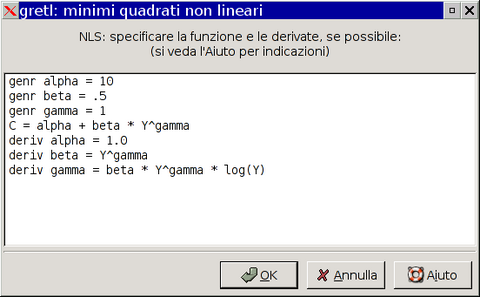
\includegraphics[scale=0.5]{figures/nls_window}
  \end{center}
  \caption{Finestra di dialogo NLS}
  \label{fig-nls-dialog}
\end{figure}


\section{Derivate analitiche e numeriche}
\label{nls-deriv}

Se si � in grado di calcolare le derivate dalla funzione di
regressione rispetto ai parametri, � consigliabile indicarle come
mostrato negli esempi precedenti. Se ci� non � possibile, \app{gretl}
calcoler� delle derivate approssimate numericamente. Le propriet�
dell'algoritmo NLS in questo caso potrebbero non essere ottimali (si
veda Section \ref{nls-accuracy}).

Se vengono fornite delle derivate analitiche, ne viene controllata la
coerenza con la funzione non lineare data. Se esse sono chiaramente
scorrette, la stima viene annullata con un messaggio di errore. Se le
derivate sono ``sospette'', viene mostrato un messaggio di
avvertimento, ma la stima prosegue.  Questo avvertimento pu� essere
causato da derivate scorrette, ma pu� anche essere dovuto a un alto
grado di collinearit� tra le derivate.

Si noti che non � possibile mischiare derivate numeriche e analitiche:
se si indicano espressioni analitiche per le derivate, occorre farlo
per tutte.

\section{Arresto della procedura}
\label{nls-toler}

La procedura di stima NLS � iterativa: l'iterazione viene arrestata si
verifica una qualunque delle seguenti condizioni: viene raggiunto un
criterio di convergenza, o si supera il massimo numero di iterazioni
impostato. Il massimo numero di iterazioni � \cmd{100*(k+1)} se
vengono fornite derivate analitiche, o \cmd{200*(k+1)} se vengono
usate derivate numeriche, dove \verb+k+ indica il numero di parametri
da stimare. Il criterio di convergenza consiste nel fatto che l'errore
relativo nella somma dei quadrati e/o l'errore relativo tra il vettore
dei coefficienti e la soluzione sia stimato inferiore a un certo
valore piccolo. Questo ``valore piccolo'' � impostato in modo
predefinito pari alla precisione della macchina elevato alla potenza
3/4, ma pu� essere impostato con il comando \cmd{genr}, usando la
variabile speciale \verb+toler+. Ad esempio

\begin{code}
genr toler = .0001
\end{code}

imposter� la tolleranza a 0.0001.

\section{Dettagli sul codice}
\label{nls-code}

Il motore sottostante la stima NLS � basato sulla suite di funzioni
\app{minpack}, disponibile su
\href{http://www.netlib.org/minpack/}{netlib.org}.  Nello specifico,
sono usate le seguenti funzioni \app{minpack}:

\begin{center}
  \begin{tabular}{ll}
    \verb+lmder+ & 
    Algoritmo Levenberg--Marquandt con derivate analitiche \\
    \verb+chkder+ & 
    Controllo delle derivate analitiche fornite \\
    \verb+lmdif+ & 
    Algoritmo Levenberg--Marquandt con derivate numeriche \\
    \verb+fdjac2+ & 
    Calcolo del Jacobiano approssimato finale se si usano le derivate 
    numeriche \\
    \verb+dpmpar+ & 
    Determinazioen della precisione della macchina \\
  \end{tabular}
\end{center}

In caso di successo nell'iterazione Levenberg--Marquandt, viene usata
una regressione Gauss--Newton per calcolare la matrice di covarianza
per le stime dei parametri. Poich� i risultati NLS sono asintotici, si
pu� discutere sulla necessit� di applicare una correzione per i gradi
di libert� nel calcolo dell'errore standard della regressione (e di
quello delle stime dei parametri). Per confrontabilit� con OLS, e
seguendo il ragionamento in Davidson e MacKinnon (1993), le stime
calcolate in \app{gretl} \emph{usano} una correzione per i gradi di
libert�.

\section{Accuratezza numerica}
\label{nls-accuracy}

La Table \ref{tab-nls} mostra i risultati dell'uso della procedura NLS
di \app{gretl} sui 27 ``Statistical Reference Dataset'' forniti dal
National Institute of Standards and Technology (NIST) statunitense,
per il test del software di regressione non lineare.\footnote{Per una
  discussione dell'accuratezza di \app{gretl} nella stima di modelli
  lineari, si veda l'appendice~\ref{app-accuracy}.} Per ogni dataset,
il file di test indicano due valori iniziali per i parametri, quindi
il test completo riporta 54 stime. Sono stati eseguiti due test
completi, uno usando derivate analitiche e uno usando approssimazioni
numeriche; in entrambi casi si � usata la tolleranza
predefinita.\footnote{I dati mostrati nella tabella derivano da una
  versione di \app{gretl} 1.0.9, compilata con \app{gcc} 3.3,
  collegata a \app{glibc} 2.3.2 ed eseguita in Linux su un PC i686
  (IBM ThinkPad A21m).}

Sulle 54 stime, \app{gretl} non riesce a produrre una soluzione in 4
casi, se vengono usate le derivate analitiche, e in 5 casi se vengono
usate le approssimazioni numeriche. Dei quattro fallimenti in modalit�
derivate analitiche, due sono dovuti alla non convergenza
dell'algoritmo Levenberg--Marquandt dopo il numero massimo di
iterazioni (su \verb+MGH09+ e \verb+Bennett5+, entrambi descritti dal
NIST come di ``alta difficolt�'') e due sono dovuti ad errori di
intervallo (valori in virgola mobile al di fuori dei limiti) occorsi
durante il calcolo del Jacobiano (su \verb+BoxBOD+ e \verb+MGH17+,
rispettivamente descritti come di ``alta difficolt�'' e di ``media
difficolt�''). In modalit� approssimazione numerica, l'ulteriore caso
di fallimento � rappresentato da \verb+MGH10+ (``alta difficolt�'',
massimo numero di iterazioni raggiunto).

La tabella mostra informazioni su vari aspetti dei test: numero di
fallimenti, numero medio di iterazioni richieste per produrre una
soluzione, e due tipi di misura dell'accuratezza dei risultati per i
parametri e per i loro errori standard.  Per ognuno dei 54 test
eseguiti in ogni modalit�, se � stata prodotta una soluzione, sono
state confrontate le stime dei parametri ottenute da \app{gretl} con i
valori certificati dal NIST. � stata definita la variabile ``numero
minimo di cifre corrette'' per una data stima come il numero di cifre
significative per cui la \emph{meno accurata} delle stime di
\app{gretl} coincide con il valore certificato. La tabella mostra i
valori medio e minimo di questa variabile, calcolati sulle stime che
hanno prodotto una soluzione; la stessa informazione � fornita per gli
errori standard stimati.\footnote{Per gli errori standard, dalle
  statistiche mostrate nella tabella, � stato escluso l'outlier
  costituito da \verb+Lanczos1+, che rappresenta un caso strano,
  composto da dati generati con un adattamento quasi esatto; gli
  errori standard sono di 9 o 10 ordini di grandezza pi� piccoli dei
  coefficienti. In questo caso \app{gretl} riesce a riprodurre gli
  errori standard solo per 3 cifre (con derivate analitiche) e per 2
  cifre (con derivate numeriche).}  

La seconda misura di accuratezza mostrata � la percentuale di casi,
tenendo conto di tutti i parametri di tutte le stime giunte a buon
fine, in cui la stima di \app{gretl} concorda con il valore
certificato per almeno 6 cifre significative, che sono mostrate in
modo predefinito nei risultati delle regressioni di \app{gretl}.

\begin{table}[htbp]
  \caption{Regressione non lineare: i test NIST}
  \label{tab-nls}
  \begin{center}
    \begin{tabular}{lcc}
      � & \textit{Derivate analitiche} 
        & \textit{Derivate numeriche} \\ [4pt]
        Falimenti in 54 test & 4 & 5\\
        Iterazioni medie & 32 & 127\\
        Media del "numero minimo di cifre corrette", & 8.120 & 6.980\\
        stima dei parametri \\
        Valore minimo del "numero minimo di cifre corrette", & 4 & 3 \\
        stima dei parametri \\
        Media del "numero minimo di cifre corrette", & 8.000 & 5.673\\
        stima degli errori standard \\
        Valore minimo del "numero minimo di cifre corrette", & 5 & 2\\
        stima degli errori standard \\
        Percentuale delle stime corrette a 6 cifre, & 96.5 & 91.9\\
        stima dei parametri \\
        Percentuale delle stime corrette a 6 cifre, & 97.7 & 77.3\\
        stima degli errori standard \\
      \end{tabular}
    \end{center}
  \end{table}

  Usando derivate analitiche, i valori dei casi peggiori sia per le
  stime dei parametri che per gli errori standard sono stati
  migliorati a 6 cifre corrette restringendo il valore di tolleranza a
  1.0e$-$14.  Usando derivate numeriche, la stessa modifica del limite
  di tolleranza ha innalzato la precisione dei valori peggiori a 5
  cifre corrette per i parametri e 3 cifre per gli errori standard, al
  costo di un fallimento in pi� nella convergenza.  

  Si noti la tendenziale superiorit� delle derivate analitiche: in
  media le soluzioni ai problemi dei test sono state ottenute con
  molte meno iterazioni e i risultati sono pi� accurati (in modo
  evidente per gli errori standard stimati). Si noti anche che i
  risultati a 6 cifre mostrati da \app{gretl} non sono affidabili al
  100 per cento per i problemi non lineari difficili (in particolare
  se si usano derivate numeriche). Tenendo presente questi limiti, la
  percentuale dei casi in cui i risultati sono accurati alla sesta
  cifra o pi� sembra sufficiente per giustificarne l'utilizzo in
  questa forma.

%%% Local Variables: 
%%% mode: latex
%%% TeX-master: "gretl-guide-it"
%%% End: 


\chapter{Maximum likelihood estimation}
\label{chap:mle}

\section{Generic ML estimation with gretl}
\label{sec:mle-intro}


Maximum likelihood estimation is a cornerstone of modern inferential
procedures. Gretl provides a way to implement this method for a wide
range of estimation problems, by use of the \texttt{mle} command. We
give here a few examples.

To give a foundation for the examples that follow, we start from a
brief reminder on the basics of ML estimation.  Given a sample of size
$T$, it is possible to define the density function\footnote{We are
  supposing here that our data are a realization of continuous random
  variables. For discrete random variables, everything continues to
  apply by referring to the probability function instead of the
  density. In both cases, the distribution may be conditional on some
  exogenous variables.} for the whole sample, namely the joint
distribution of all the observations $f(\mathbf{Y} ; \theta)$, where
$\mathbf{Y} = \left\{ y_1, \ldots, y_T \right\}$.  Its shape is
determined by a $k$-vector of unknown parameters $\theta$, which we
assume is contained in a set $\Theta$, and which can be used to
evaluate the probability of observing a sample with any given
characteristics.

After observing the data, the values $\mathbf{Y}$ are given, and this
function can be evaluated for any legitimate value of $\theta$. In
this case, we prefer to call it the \emph{likelihood} function; the
need for another name stems from the fact that this function works as
a density when we use the $y_t$s as arguments and $\theta$ as
parameters, whereas in this context $\theta$ is taken as the
function's argument, and the data $\mathbf{Y}$ only have the role of
determining its shape.

In standard cases, this function has a unique maximum.  The location
of the maximum is unaffected if we consider the logarithm of the
likelihood (or log-likelihood for short): this function will be
denoted as
\[
  \LogLik(\theta) = \log  f(\mathbf{Y}; \theta)
\] 
The log-likelihood functions that gretl can handle are those where
$\LogLik(\theta)$ can be written as
\[
  \LogLik(\theta) = \sum_{t=1}^T \ell_t(\theta)
\] 
which is true in most cases of interest. The functions $\ell_t(\theta)$
are called the log-likelihood contributions.

Moreover, the location of the maximum is obviously determined by the
data $\mathbf{Y}$. This means that the value
\begin{equation}
  \label{eq:maxlik}
  \hat{\theta}(\mathbf{Y}) = \argmax_{\theta \in \Theta} \LogLik(\theta)
\end{equation}
is some function of the observed data (a statistic), which has the
property, under mild conditions, of being a consistent, asymptotically
normal and asymptotically efficient estimator of $\theta$.

Sometimes it is possible to write down explicitly the function
$\hat{\theta}(\mathbf{Y})$; in general, it need not be so. In these
circumstances, the maximum can be found by means of numerical
techniques. These often rely on the fact that the log-likelihood is a
smooth function of $\theta$, and therefore on the maximum its partial
derivatives should all be 0.  The \textsl{gradient vector}, or
\textsl{score vector}, is a function that enjoys many interesting
statistical properties in its own right; it will be denoted here as
$\mathbf{g}(\theta)$.  It is a $k$-vector with typical element
\[
g_i(\theta) = \frac{\partial\LogLik(\theta)}{\partial\theta_i} 
  = \sum_{t=1}^T \frac{\partial\ell_t(\theta)}{\partial\theta_i}
\]

Gradient-based methods can be briefly illustrated as follows:

\begin{enumerate}
\item pick a point $\theta_0 \in \Theta$;
\item evaluate $\mathbf{g}(\theta_0)$;
\item if $\mathbf{g}(\theta_0)$ is ``small'', stop. Otherwise, compute
  a direction vector $d(\mathbf{g}(\theta_0))$;
\item evaluate $\theta_1 = \theta_0 + d(\mathbf{g}(\theta_0))$;
\item substitute $\theta_0$ with $\theta_1$;
\item restart from 2.
\end{enumerate}

Many algorithms of this kind exist; they basically differ from one
another in the way they compute the direction vector
$d(\mathbf{g}(\theta_0))$, to ensure that $\LogLik(\theta_1) >
\LogLik(\theta_0)$ (so that we eventually end up on the maximum).

The default method gretl uses to maximize the log-likelihood is a
gradient-based algorithm known as the \textbf{BFGS} (Broyden,
Fletcher, Goldfarb and Shanno) method. This technique is used in most
econometric and statistical packages, as it is well-established and
remarkably powerful. Clearly, in order to make this technique
operational, it must be possible to compute the vector
$\mathbf{g}(\theta)$ for any value of $\theta$. In some cases this
vector can be written explicitly as a function of $\mathbf{Y}$. If
this is not possible or too difficult the gradient may be evaluated
numerically. The alternative \textbf{Newton-Raphson} algorithm is also
available. This method is more effective under some circumstances but
is also more fragile; see section \ref{sec:mle-adv} and chapter
\ref{chap:numerical} for details.\footnote{Note that some of the
  statements made below (for example, regarding estimation of the
  covariance matrix) have to be modified when Newton's method is
  used.}

The choice of the starting value, $\theta_0$, is crucial in some contexts
and inconsequential in others. In general, however, it is
advisable to start the algorithm from ``sensible'' values whenever
possible. If a consistent estimator is available, this is usually a
safe and efficient choice: this ensures that in large samples the
starting point will be likely close to $\hat{\theta}$ and convergence
can be achieved in few iterations. 

The maximum number of iterations allowed for the BFGS procedure, and
the relative tolerance for assessing convergence, can be adjusted
using the \cmd{set} command: the relevant variables are
\verb+bfgs_maxiter+ (default value 500) and \verb+bfgs_toler+ (default
value, the machine precision to the power 3/4).

\subsection{Covariance matrix and standard errors}

By default the covariance matrix of the parameter estimates is
based on the Outer Product of the Gradient (OPG).  That is,
\begin{equation}
  \label{eq:OPGmat}
  \widehat{\mbox{Var}}_{\mbox{\scriptsize OPG}}(\hat{\theta}) =
  \left(G'(\hat{\theta}) G(\hat{\theta}) \right)^{-1}
\end{equation}
where $G(\hat{\theta})$ is the $T \times k$ matrix of contributions to
the gradient.  Two other options are available.  If the
\option{hessian} flag is given, the covariance matrix is computed from
a numerical approximation to the Hessian at convergence.  If the
\option{robust} option is selected, the quasi-ML ``sandwich''
estimator is used:
\[
\widehat{\mbox{Var}}_{\mbox{\scriptsize QML}}(\hat{\theta}) = H(\hat{\theta})^{-1}
  G'(\hat{\theta}) G(\hat{\theta}) H(\hat{\theta})^{-1}
\]
where $H$ denotes the numerical approximation to the Hessian.

Cluster-robust estimation is also available: in order to activate it,
use the \option{cluster=}\emph{\texttt{clustvar}}, where \cmd{clustvar}
should be a discrete series. See section \ref{sec:vcv-cluster} for
more details.

Note, however, that if the log-likelihood function supplied by the
user just returns a scalar value---as opposed to a series or vector
holding per-observation contributions---then the OPG method is not
applicable and so the covariance matrix must be estimated via a
numerical approximation to the Hessian.

\section{Gamma estimation}
\label{sec:ml-gamma}

Suppose we have a sample of $T$ independent and identically
distributed observations from a Gamma distribution. The density
function for each observation $x_t$ is
\begin{equation}
  \label{eq:gammadens}
  f(x_t) = \frac{\alpha^p}{\Gamma(p)} x_t^{p-1} \exp\left({-\alpha
      x_t}\right)
\end{equation}
The log-likelihood for the entire sample can be written as the
logarithm of the joint density of all the observations. Since these
are independent and identical, the joint density is the product of the
individual densities, and hence its log is
\begin{equation}
  \label{eq:gammaloglik}
  \LogLik(\alpha, p) = \sum_{t=1}^T \log \left[ \frac{\alpha^p}{\Gamma(p)} x_t^{p-1} \exp\left({-\alpha
      x_t}\right) \right] = 
      \sum_{t=1}^T \ell_t
\end{equation}
where 
\[
  \ell_t = p \cdot \log (\alpha x_t) - \gamma(p) - \log x_t - \alpha x_t
\]
and $\gamma(\cdot)$ is the log of the gamma function.  In order to
estimate the parameters $\alpha$ and $p$ via ML, we need to maximize
(\ref{eq:gammaloglik}) with respect to them. The corresponding
gretl code snippet is

\begin{code}
scalar alpha = 1
scalar p = 1

mle logl =  p*ln(alpha * x) - lngamma(p) - ln(x) - alpha * x 
  params alpha p
end mle 
\end{code}

The first two statements

\begin{code}
alpha = 1
p = 1
\end{code}

are necessary to ensure that the variables \texttt{alpha} and
\texttt{p} exist before the computation of \texttt{logl} is
attempted. Inside the \texttt{mle} block these variables (which could
be either scalars, vectors or a combination of the two --- see below
for an example) are identified as the parameters that should be
adjusted to maximize the likelihood via the \texttt{params} keyword.
Their values will be changed by the execution of the \texttt{mle}
command; upon successful completion, they will be replaced by the ML
estimates. The starting value is 1 for both; this is arbitrary and
does not matter much in this example (more on this later).

The above code can be made more readable, and marginally more
efficient, by defining a variable to hold $\alpha \cdot x_t$. This
command can be embedded in the \texttt{mle} block as follows:
\begin{code}
mle logl =  p*ln(ax) - lngamma(p) - ln(x) - ax 
  series ax = alpha*x
  params alpha p
end mle 
\end{code}
The variable \texttt{ax} is not added to the \texttt{params} list,
of course, since it is just an auxiliary variable to facilitate
the calculations.  You can insert as many such auxiliary lines
as you require before the \texttt{params} line, with the restriction
that they must contain either (a) commands to generate series,
scalars or matrices or (b) print commands (which may be used to
aid in debugging).

In a simple example like this, the choice of the starting values is
almost inconsequential; the algorithm is likely to converge no
matter what the starting values are. However, consistent
method-of-moments estimators of $p$ and $\alpha$ can be simply
recovered from the sample mean $m$ and variance $V$: since it can be
shown that
\[
  E(x_t) = p/\alpha \qquad  V(x_t) = p/\alpha^2
\]
it follows that the following estimators 
\begin{eqnarray*}
  \bar{\alpha} & = &  m/V \\
  \bar{p} & = & m \cdot \bar{\alpha} 
\end{eqnarray*}
are consistent, and therefore suitable to be used as starting point
for the algorithm.  The gretl script code then becomes
\begin{code}
scalar m = mean(x)
scalar alpha = m/var(x)
scalar p = m*alpha

mle logl =  p*ln(ax) - lngamma(p) - ln(x) - ax 
  series ax = alpha*x
  params alpha p
end mle 
\end{code}

Another thing to note is that sometimes parameters are constrained
within certain boundaries: in this case, for example, both $\alpha$
and $p$ must be positive numbers. Gretl does not check for this:
it is the user's responsibility to ensure that the function is
always evaluated at an admissible point in the parameter space during
the iterative search for the maximum. An effective technique is to
define a variable for checking that the parameters are admissible and
setting the log-likelihood as undefined if the check fails. An
example, which uses the conditional assignment operator, follows:
\begin{code}
scalar m = mean(x)
scalar alpha = m/var(x)
scalar p = m*alpha

mle logl = check ? p*ln(ax) - lngamma(p) - ln(x) - ax : NA
  series ax = alpha*x
  scalar check = (alpha>0) && (p>0)
  params alpha p
end mle 
\end{code}

\section{Stochastic frontier cost function}
\label{sec:frontier}

\emph{%
Note: this section has the only purpose of illustrating the \cmd{mle}
command. For the estimation of stochastic frontier cost or production
functions, you may want to use the \package{frontier} function package.}

When modeling a cost function, it is sometimes worthwhile to
incorporate explicitly into the statistical model the notion that
firms may be inefficient, so that the observed cost deviates from the
theoretical figure not only because of unobserved heterogeneity
between firms, but also because two firms could be operating at a
different efficiency level, despite being identical under all other
respects. In this case we may write
\[
  C_i = C^*_i + u_i + v_i
\]
where $C_i$ is some variable cost indicator, $C_i^*$ is its
``theoretical'' value, $u_i$ is a zero-mean disturbance term and $v_i$
is the inefficiency term, which is supposed to be nonnegative by its
very nature. A linear specification for $C_i^*$ is often chosen. For
example, the Cobb--Douglas cost function arises when $C_i^*$ is a
linear function of the logarithms of the input prices and the output
quantities.

The \emph{stochastic frontier} model is a linear model of the form
$y_i = x_i \beta + \varepsilon_i$ in which the error term
$\varepsilon_i$ is the sum of $u_i$ and $v_i$.  

A common postulate is that $u_i \sim N(0,\sigma_u^2)$ and
$v_i \sim \left|N(0,\sigma_v^2)\right|$. If independence between $u_i$
and $v_i$ is also assumed, then it is possible to show that the
density function of $\varepsilon_i$ has the form:
\begin{equation}
  \label{eq:frontdens}
  f(\varepsilon_i) = 
   \sqrt{\frac{2}{\pi}} 
   \Phi\left(\frac{\lambda \varepsilon_i}{\sigma}\right)
   \frac{1}{\sigma} \phi\left(\frac{\varepsilon_i}{\sigma}\right)
\end{equation}
where $\Phi(\cdot)$ and $\phi(\cdot)$ are, respectively, the distribution and density
function of the standard normal, $\sigma =
\sqrt{\sigma^2_u + \sigma^2_v}$ and $\lambda = \frac{\sigma_u}{\sigma_v}$.

As a consequence, the log-likelihood for one observation takes the
form (apart form an irrelevant constant)
\[
  \ell_t = 
  \log\Phi\left(\frac{\lambda \varepsilon_i}{\sigma}\right) -
  \left[ \log(\sigma) + \frac{\varepsilon_i^2}{2 \sigma^2} \right]
\]
Therefore, a Cobb--Douglas cost function with stochastic frontier is the
model described by the following equations: 
\begin{eqnarray*}
  \log C_i & = & \log C^*_i + \varepsilon_i \\
  \log C^*_i & = & c + \sum_{j=1}^m \beta_j \log y_{ij} + \sum_{j=1}^n \alpha_j \log p_{ij} \\
  \varepsilon_i & = & u_i + v_i \\
  u_i & \sim & N(0,\sigma_u^2) \\
  v_i & \sim & \left|N(0,\sigma_v^2)\right| 
\end{eqnarray*}

In most cases, one wants to ensure that the homogeneity of the cost
function with respect to the prices holds by construction. Since this
requirement is equivalent to $\sum_{j=1}^n \alpha_j = 1$, the above
equation for $C^*_i$ can be rewritten as

\begin{equation}
  \label{eq:CobbDouglasFrontier}
  \log C_i - \log p_{in}  = c + \sum_{j=1}^m \beta_j \log y_{ij} +
  \sum_{j=2}^n \alpha_j (\log p_{ij} - \log p_{in})  + \varepsilon_i
\end{equation}

The above equation could be estimated by OLS, but it would suffer from
two drawbacks: first, the OLS estimator for the intercept $c$ is
inconsistent because the disturbance term has a non-zero expected
value; second, the OLS estimators for the other parameters are
consistent, but inefficient in view of the non-normality of
$\varepsilon_i$. Both issues can be addressed by estimating
(\ref{eq:CobbDouglasFrontier}) by maximum likelihood. Nevertheless,
OLS estimation is a quick and convenient way to provide starting
values for the MLE algorithm.

Listing \ref{cost-estimation} shows how to implement the model
described so far. The \texttt{banks91} file contains part of the data
used in \citet*{lucchetti01}.

\begin{script}[htbp]
  \scriptcaption{Estimation of stochastic frontier cost function (with
    scalar parameters)}
  \label{cost-estimation}
\begin{scode}
open banks91.gdt

# transformations
series cost = ln(VC)
series q1 = ln(Q1)
series q2 = ln(Q2)
series p1 = ln(P1)
series p2 = ln(P2)
series p3 = ln(P3)

# Cobb-Douglas cost function with homogeneity restrictions
# (for initialization)
series rcost = cost - p1
series rp2 = p2 - p1
series rp3 = p3 - p1

ols rcost const q1 q2 rp2 rp3

# Cobb-Douglas cost function with homogeneity restrictions 
# and inefficiency 

scalar b0 = $coeff(const)
scalar b1 = $coeff(q1)
scalar b2 = $coeff(q2)
scalar b3 = $coeff(rp2)
scalar b4 = $coeff(rp3)

scalar su = 0.1
scalar sv = 0.1

mle logl = ln(cnorm(e*lambda/ss)) - (ln(ss) + 0.5*(e/ss)^2)
  scalar ss = sqrt(su^2 + sv^2)
  scalar lambda = su/sv
  series e = rcost - b0*const - b1*q1 - b2*q2 - b3*rp2 - b4*rp3
  params b0 b1 b2 b3 b4 su sv
end mle
\end{scode}
\end{script}

The script in example \ref{cost-estimation} is relatively easy to
modify to show how one can use vectors (that is, 1-dimensional
matrices) for storing the parameters to optimize: example
\ref{cost-estimation-vec} holds essentially the same script in which
the parameters of the cost function are stored together in a
vector. Of course, this makes also possible to use variable lists and
other refinements which make the code more compact and readable.

\begin{script}[htbp]
  \scriptcaption{Estimation of stochastic frontier cost function (with
    matrix parameters)}
  \label{cost-estimation-vec}
\begin{scode}
open banks91.gdt

# transformations
series cost = ln(VC)
series q1 = ln(Q1)
series q2 = ln(Q2)
series p1 = ln(P1)
series p2 = ln(P2)
series p3 = ln(P3)

# Cobb-Douglas cost function with homogeneity restrictions
# (for initialization)
series rcost = cost - p1
series rp2 = p2 - p1
series rp3 = p3 - p1
list X = const q1 q2 rp2 rp3

ols rcost X
X = const q1 q2 rp2 rp3
# Cobb-Douglas cost function with homogeneity restrictions 
# and inefficiency 

matrix b = $coeff
scalar su = 0.1
scalar sv = 0.1

mle logl = ln(cnorm(e*lambda/ss)) - (ln(ss) + 0.5*(e/ss)^2)
  scalar ss = sqrt(su^2 + sv^2)
  scalar lambda = su/sv
  series e = rcost - lincomb(X, b)
  params b su sv
end mle
\end{scode}
\end{script}

\section{GARCH models}
\label{sec:garch}

GARCH models are handled by gretl via a native function. However, it is
instructive to see how they can be estimated through the \texttt{mle}
command.\footnote{The \package{gig} addon, which handles other variants
of conditionally heteroskedastic models, uses \texttt{mle} as its
internal engine.}

The following equations provide the simplest example of a GARCH(1,1)
model:
\begin{eqnarray*}
  y_t & = & \mu + \varepsilon_t \\
  \varepsilon_t & = & u_t \cdot \sigma_t \\
  u_t & \sim & N(0,1) \\
  h_t & = & \omega + \alpha \varepsilon^2_{t-1} + \beta h_{t-1}.
\end{eqnarray*}
Since the variance of $y_t$ depends on past values, writing down the
log-likelihood function is not simply a matter of summing the log
densities for individual observations. As is common in time series
models, $y_t$ cannot be considered independent of the other
observations in our sample, and consequently the density function for
the whole sample (the joint density for all observations) is not just
the product of the marginal densities.

Maximum likelihood estimation, in these cases, is achieved by
considering \emph{conditional} densities, so what we maximize is a
conditional likelihood function. If we define the information set at
time $t$ as
\[
  F_t = \left\{ y_t, y_{t-1}, \ldots \right\} ,
\]
then the density of $y_t$ conditional on $F_{t-1}$ is normal:
\[
  y_t | F_{t-1} \sim N\left[ \mu, h_{t} \right].
\]

By means of the properties of conditional distributions, the joint
density can be factorized as follows
\[
  f(y_t, y_{t-1}, \ldots) = \left[ \prod_{t=1}^T f(y_t |F_{t-1})
  \right] \cdot f(y_0)
\]
If we treat $y_0$ as fixed, then the term $f(y_0)$ does not depend on
the unknown parameters, and therefore the conditional log-likelihood
can then be written as the sum of the individual contributions as
\begin{equation}
  \label{eq:garchloglik}
  \LogLik(\mu,\omega,\alpha,\beta) = \sum_{t=1}^T \ell_t
\end{equation}
where 
\[
  \ell_t = \log \left[ \frac{1}{\sqrt{h_t}} \phi\left( \frac{y_t - \mu}{\sqrt{h_t}}
    \right) \right] = 
    - \frac{1}{2} \left[ \log(h_t) + \frac{(y_t - \mu)^2}{h_t} \right]
\]

The following script shows a simple application of this technique,
which uses the data file \texttt{djclose}; it is one of the example
dataset supplied with gretl and contains daily data from the Dow Jones
stock index.

\begin{code}
open djclose

series y = 100*ldiff(djclose)

scalar mu = 0.0
scalar omega = 1
scalar alpha = 0.4
scalar beta = 0.0

mle ll = -0.5*(log(h) + (e^2)/h)
  series e = y - mu
  series h = var(y)
  series h = omega + alpha*(e(-1))^2 + beta*h(-1)
  params mu omega alpha beta
end mle
\end{code}

\section{Analytical derivatives}
\label{sec:anal-der}

Computation of the score vector is essential for the working of the
BFGS method. In all the previous examples, no explicit formula for the
computation of the score was given, so the algorithm was fed
numerically evaluated gradients. Numerical computation of the score for
the $i$-th parameter is performed via a finite approximation of the
derivative, namely
\[
  \pder{\LogLik(\theta_1, \ldots, \theta_n)}{\theta_i} \simeq 
  \frac{\LogLik(\theta_1, \ldots, \theta_i + h, \ldots, \theta_n) -
    \LogLik(\theta_1, \ldots, \theta_i - h, \ldots, \theta_n)}{2h}
\]
where $h$ is a small number. 

In many situations, this is rather efficient and accurate. A better
approximation to the true derivative may be obtained by forcing
\cmd{mle} to use a technique known as \emph{Richardson Extrapolation},
which gives extremely precise results, but is considerably more
CPU-intensive. This feature may be turned on by using the \cmd{set}
command as in
\begin{code}
  set bfgs_richardson on
\end{code}

However, one might want to avoid the approximation and specify an
exact function for the derivatives. As an example, consider the
following script:
%
\begin{code}
nulldata 1000

series x1 = normal()
series x2 = normal()
series x3 = normal()

series ystar = x1 + x2 + x3 + normal()
series y = (ystar > 0)

scalar b0 = 0
scalar b1 = 0
scalar b2 = 0
scalar b3 = 0

mle logl = y*ln(P) + (1-y)*ln(1-P)
  series ndx = b0 + b1*x1 + b2*x2 + b3*x3
  series P = cnorm(ndx)
  params b0 b1 b2 b3
end mle --verbose
\end{code}

Here, 1000 data points are artificially generated for an ordinary
probit model:\footnote{Again, gretl does provide a native
  \texttt{probit} command (see section \ref{sec:logit-probit}), but a
  probit model makes for a nice example here.} $y_t$ is a binary
variable, which takes the value 1 if $y_t^* = \beta_1 x_{1t} + \beta_2
x_{2t} + \beta_3 x_{3t} + \varepsilon_t > 0$ and 0 otherwise.
Therefore, $y_t = 1$ with probability $\Phi(\beta_1 x_{1t} + \beta_2
x_{2t} + \beta_3 x_{3t}) = \pi_t$.  The probability function for one
observation can be written as
\[
  P(y_t) = \pi_t^{y_t} ( 1 -\pi_t )^{1-y_t}
\]
Since the observations are independent and identically distributed,
the log-likelihood is simply the sum of the individual
contributions. Hence
\[
  \LogLik = \sum_{t=1}^T y_t \log(\pi_t) + (1 - y_t) \log(1 - \pi_t)
\]
The \option{verbose} switch at the end of the \texttt{end mle}
statement produces a detailed account of the iterations done by the
BFGS algorithm.

In this case, numerical differentiation works rather well;
nevertheless, computation of the analytical score is straightforward,
since the derivative $\pder{\LogLik}{\beta_i}$ can be written as
\[
  \pder{\LogLik}{\beta_i} = \pder{\LogLik}{\pi_t} \cdot \pder{\pi_t}{\beta_i}
\]
via the chain rule, and it is easy to see that
\begin{eqnarray*}
  \pder{\LogLik}{\pi_t} & = & \frac{y_t}{\pi_t} - \frac{1 - y_t}{1 -
    \pi_t} \\
  \pder{\pi_t}{\beta_i} & = & \phi(\beta_1 x_{1t} + \beta_2 x_{2t} +
  \beta_3 x_{3t}) \cdot x_{it}
\end{eqnarray*}

The \texttt{mle} block in the above script can therefore be modified
as follows:
%
\begin{code}
mle logl = y*ln(P) + (1-y)*ln(1-P)
  series ndx = b0 + b1*x1 + b2*x2 + b3*x3
  series P = cnorm(ndx)
  series m = dnorm(ndx)*(y/P - (1-y)/(1-P))
  deriv b0 = m
  deriv b1 = m*x1
  deriv b2 = m*x2
  deriv b3 = m*x3
end mle --verbose
\end{code}

Note that the \texttt{params} statement has been replaced by a series
of \texttt{deriv} statements; these have the double function of
identifying the parameters over which to optimize and providing an
analytical expression for their respective score elements.

\section{Debugging ML scripts}
\label{sec:mle-debug}

We have discussed above the main sorts of statements that are
permitted within an \texttt{mle} block, namely 
%
\begin{itemize}
\item auxiliary commands to generate helper variables;
\item \texttt{deriv} statements to specify the gradient with respect
  to each of the parameters; and
\item a \texttt{params} statement to identify the parameters in case
  analytical derivatives are not given.
\end{itemize}

For the purpose of debugging ML estimators one additional sort of
statement is allowed: you can print the value of a relevant variable
at each step of the iteration.  This facility is more restricted then
the regular \texttt{print} command.  The command word \texttt{print}
should be followed by the name of just one variable (a scalar, series
or matrix).

In the last example above a key variable named \texttt{m} was
generated, forming the basis for the analytical derivatives.  To track
the progress of this variable one could add a print statement within
the ML block, as in
%
\begin{code}
series m = dnorm(ndx)*(y/P - (1-y)/(1-P))
print m
\end{code}

\section{Using functions}
\label{sec:mle-func}

The \texttt{mle} command allows you to estimate models that
gretl does not provide natively: in some cases, it may be a good
idea to wrap up the \texttt{mle} block in a user-defined function (see
Chapter \ref{chap:functions}), so as to extend gretl's
capabilities in a modular and flexible way.

As an example, we will take a simple case of a model that gretl
does not yet provide natively: the zero-inflated Poisson model, or ZIP
for short.\footnote{The actual ZIP model is in fact a bit more general
than the one presented here. The specialized version discussed in this
section was chosen for the sake of simplicity. For futher details, see
\cite{greene03}.} In this model, we assume that we observe a mixed
population: for some individuals, the variable $y_t$ is (conditionally
on a vector of exogenous covariates $x_t$) distributed as a Poisson
random variate; for some others, $y_t$ is identically 0. The trouble
is, we don't know which category a given individual belongs to.  

For instance, suppose we have a sample of women, and the variable $y_t$
represents the number of children that woman $t$ has. There may be a
certain proportion, $\alpha$, of women for whom $y_t = 0$ with certainty
(maybe out of a personal choice, or due to physical impossibility). 
But there may be other women for whom $y_t = 0$ just as a matter of
chance --- they haven't happened to have any children at the time
of observation.

In formulae:
\begin{eqnarray*}
  P(y_t = k | x_t) & = & \alpha d_t + (1 - \alpha) 
  \left[e^{-\mu_t} \frac{\mu_t^{y_t}}{y_t!}\right] \\
    \mu_t & = & \exp(x_t \beta) \\
    d_t & = & 
    \left\{ 
      \begin{array}{ll} 
        1 & \mathrm{for} \quad y_t = 0 \\ 
        0 & \mathrm{for} \quad y_t > 0 
      \end{array}
    \right. 
\end{eqnarray*}

Writing a \texttt{mle} block for this model is not difficult:
\begin{code}
mle ll = logprob
  series xb = exp(b0 + b1 * x)
  series d = (y=0)
  series poiprob = exp(-xb) * xb^y / gamma(y+1)
  series logprob = (alpha>0) && (alpha<1) ? \
    log(alpha*d + (1-alpha)*poiprob) : NA
  params alpha b0 b1
end mle -v
\end{code}

However, the code above has to be modified each time we change our
specification by, say, adding an explanatory variable.  Using
functions, we can simplify this task considerably and eventually be
able to write something easy like
\begin{code}
list X = const x
zip(y, X)
\end{code}

\begin{script}[htbp]
  \scriptcaption{Zero-inflated Poisson Model -- user-level function}
  \label{mle-zip-main}
\begin{scode}
/*
  user-level function: estimate the model and print out
  the results
*/
function void zip(series y, list X)
    matrix coef_stde = zip_estimate(y, X)
    printf "\nZero-inflated Poisson model:\n"
    string parnames = "alpha,"
    string parnames += varname(X)
    modprint coef_stde parnames
end function
\end{scode}
\end{script}

Let's see how this can be done.  First we need to define a function
called \texttt{zip()} that will take two arguments: a dependent
variable \texttt{y} and a list of explanatory variables \texttt{X}. An
example of such function can be seen in script~\ref{mle-zip-main}. By
inspecting the function code, you can see that the actual estimation
does not happen here: rather, the \texttt{zip()} function merely
uses the built-in \cmd{modprint} command to print out the results
coming from another user-written function, namely
\texttt{zip\_estimate()}.

\begin{script}[htbp]
  \scriptcaption{Zero-inflated Poisson Model --- internal functions}
  \label{mle-zip-inc}
\begin{scode}
/* compute log probabilities for the plain Poisson model */
function series ln_poi_prob(series y, list X, matrix beta)
    series xb = lincomb(X, beta)
    return -exp(xb) + y*xb - lngamma(y+1)
end function  

/* compute log probabilities for the zero-inflated Poisson model */
function series ln_zip_prob(series y, list X, matrix beta, scalar p0)
    # check if the probability is in [0,1]; otherwise, return NA
    if p0 > 1 || p0 < 0
        series ret = NA
    else
        series ret = ln_poi_prob(y, X, beta) + ln(1-p0)
        series ret = y==0 ? ln(p0 + exp(ret)) : ret
    endif
    return ret
end function  

/* do the actual estimation (silently) */
function matrix zip_estimate(series y, list X)
    # initialize alpha to a "sensible" value: half the frequency
    # of zeros in the sample
    scalar alpha = mean(y==0)/2
    # initialize the coeffs (we assume the first explanatory 
    # variable is the constant here)
    matrix coef = zeros(nelem(X), 1)
    coef[1] = mean(y) / (1-alpha)
    # do the actual ML estimation
    mle ll = ln_zip_prob(y, X, coef, alpha)
        params alpha coef
    end mle --hessian --quiet
    return $coeff ~ $stderr
end function
\end{scode}
\end{script}

The function \texttt{zip\_estimate()} is not meant to be executed
directly; it just contains the number-crunching part of the job, whose
results are then picked up by the end function \texttt{zip()}. In
turn, \texttt{zip\_estimate()} calls other user-written functions to
perform other tasks. The whole set of ``internal'' functions is shown
in the panel \ref{mle-zip-inc}.

All the functions shown in \ref{mle-zip-main} and \ref{mle-zip-inc} can
be stored in a separate \texttt{inp} file and executed once, at the
beginning of our job, by means of the \texttt{include}
command.  Assuming the name of this script file is
\texttt{zip\_est.inp}, the following is an example script which
(a) includes the script file, (b) generates a simulated dataset,
and (c) performs the estimation of a ZIP model on the artificial data.

\begin{code}
set verbose off

# include the user-written functions
include zip_est.inp

# generate the artificial data
nulldata 1000
set seed 732237
scalar truep = 0.2
scalar b0 = 0.2
scalar b1 = 0.5
series x = normal()
series y = (uniform()<truep) ? 0 : randgen(p, exp(b0 + b1*x))
list X = const x

# estimate the zero-inflated Poisson model
zip(y, X)
\end{code}

The results are as follows:

\begin{code}
Zero-inflated Poisson model:

             coefficient   std. error   z-stat   p-value 
  -------------------------------------------------------
  alpha       0.209738     0.0261746     8.013   1.12e-15 ***
  const       0.167847     0.0449693     3.732   0.0002   ***
  x           0.452390     0.0340836    13.27    3.32e-40 ***
\end{code}

A further step may then be creating a function package for accessing
your new \texttt{zip()} function via gretl's graphical interface. For
details on how to do this, see section \ref{sec:func-packages}.

\section{Advanced use of \texttt{mle}: functions, analytical
  derivatives, algorithm choice}
\label{sec:mle-adv}

All the techniques decribed in the previous sections may be combined,
and \cmd{mle} can be used for solving non-standard estimation problems
(provided, of course, that one chooses maximum likelihood as the
preferred inference method).

The strategy that, as of this writing, has proven most successful in
designing scripts for this purpose is:
\begin{itemize}
\item Modularize your code as much as possible.
\item Use analytical derivatives whenever possible.
\item Choose your optimization method wisely.
\end{itemize}

In the rest of this section, we will expand on the probit example of
section \ref{sec:anal-der} to give the reader an idea of what a
``heavy-duty'' application of \cmd{mle} looks like. Most of the code
fragments come from \verb|mle-advanced.inp|, which is one of the
sample scripts supplied with the standard installation of gretl
(see under \emph{File $>$ Script files $>$ Practice File}).

\subsection{BFGS with and without analytical derivatives}
\label{sec:mle-adv-bfgs}

The example in section \ref{sec:anal-der} can be made more general by
using matrices and user-written functions. Consider the following code
fragment:
\begin{code}
list X = const x1 x2 x3
matrix b = zeros(nelem(X),1)

mle logl = y*ln(P) + (1-y)*ln(1-P)
    series ndx = lincomb(X, b)
    series P = cnorm(ndx)
    params b
end mle
\end{code}

In this context, the fact that the model we are estimating has four
explanatory variables is totally incidental: the code is written in
such a way that we could change the content of the list \texttt{X}
without having to make any other modification. This was made possible
by:
\begin{enumerate}
\item gathering the parameters to estimate into a single vector $b$
  rather than using separate scalars;
\item using the \texttt{nelem()} function to initialize $b$, so that
  its dimension is kept track of automatically;
\item using the \texttt{lincomb()} function to compute the index
  function.
\end{enumerate}

A parallel enhancement could be achieved in the case of analytically
computed derivatives: since $b$ is now a vector, \cmd{mle} expects the
argument to the \cmd{deriv} keyword to be a matrix, in which each
column is the partial derivative to the corresponding element of
$b$. It is useful to re-write the score for the $i$-th observation as
\begin{equation}
  \label{eq:mle-probscore}
  \pder{\LogLik_i}{\beta} = m_i \mathbf{x}_i'
\end{equation}
where $m_i$ is the ``signed Mills' ratio'', that is 
\[
m_i = y_i \frac{\phi(\mathbf{x}_i'\beta)}{\Phi(\mathbf{x}_i'\beta)} - 
(1-y_i) \frac{\phi(\mathbf{x}_i'\beta)}{1 - \Phi(\mathbf{x}_i'\beta)} ,
\]
which was computed in section \ref{sec:anal-der} via
\begin{code}
  series P = cnorm(ndx)
  series m = dnorm(ndx)*(y/P - (1-y)/(1-P))
\end{code}
Here, we will code it in a somewhat terser way as
\begin{code}
  series m = y ? invmills(-ndx) : -invmills(ndx)
\end{code}
and make use of the conditional assignment operator and of the
specialized function \cmd{invmills()} for efficiency.  Building the
score matrix is now easily achieved via
\begin{code}
mle logl = y*ln(P) + (1-y)*ln(1-P)
    series ndx = lincomb(X, b)
    series P = cnorm(ndx)
    series m = y ? invmills(-ndx) : -invmills(ndx)
    matrix mX = {X}
    deriv b = mX .* {m}
end mle
\end{code}
in which the \verb|{}| operator was used to turn series and lists into
matrices (see chapter \ref{chap:matrices}). However, proceeding in
this way for more complex models than probit may imply inserting into
the \cmd{mle} block a long series of instructions; the example above
merely happens to be short because the score matrix for the probit
model is very easy to write in matrix form.

A better solution is writing a user-level function to compute the
score and using that inside the \cmd{mle} block, as in
\begin{code}
function matrix score(matrix b, series y, list X)
    series ndx = lincomb(X, b)
    series m = y ? invmills(-ndx) : -invmills(ndx)
    return {m} .* {X}
end function
    
[...]

mle logl = y*ln(P) + (1-y)*ln(1-P)
    series ndx = lincomb(X, b)
    series P = cnorm(ndx)
    deriv b = score(b, y, X)
end mle
\end{code}
In this way, no matter how complex the computation of the score is,
the \cmd{mle} block remains nicely compact.

\subsection{Newton's method and the analytical Hessian}
\label{sec:mle-adv-hessian}

As mentioned above, gretl offers the user the option of using
Newton's method for maximizing the log-likelihood. In terms of the
notation used in section \ref{sec:mle-intro}, the direction for
updating the inital parameter vector $\theta_0$ is given by
\begin{equation}
  \label{eq:mle-newton}
  d\left[\mathbf{g}(\theta_0)\right] = -\lambda
  \mathbf{H}(\theta_0)^{-1}\mathbf{g}(\theta_0) ,
\end{equation}
where $\mathbf{H}(\theta)$ is the Hessian of the total loglikelihood
computed at $\theta$ and $0 < \lambda < 1$ is a scalar called the
\emph{step length}.

The above expression makes a few points clear:
\begin{enumerate}
\item At each step, it must be possible to compute not only the score
  $\mathbf{g}(\theta)$, but also its derivative $\mathbf{H}(\theta)$;
\item the matrix $\mathbf{H}(\theta)$ should be nonsingular;
\item it is assumed that for some positive value of $\lambda$,
  $\LogLik(\theta_1) > \LogLik(\theta_0)$; in other words, that going
  in the direction $d\left[\mathbf{g}(\theta_0)\right]$ leads upwards
  for some step length.
\end{enumerate}

The strength of Newton's method lies in the fact that, if the
loglikelihood is globally concave, then \eqref{eq:mle-newton} enjoys
certain optimality properties and the number of iterations required to
reach the maximum is often much smaller than it would be with other
methods, such as BFGS. However, it may have some disadvantages: for a
start, the Hessian $\mathbf{H}(\theta)$ may be difficult or very
expensive to compute; moreover, the loglikelihood may not be globally
concave, so for some values of $\theta$, the matrix
$\mathbf{H}(\theta)$ is not negative definite or perhaps even
singular.  Those cases are handled by gretl's implementation of
Newton's algorithm by means of several heuristic
techniques\footnote{The gist to it is that, if $\mathbf{H}$ is not
  negative definite, it is substituted by $k \cdot
  \mathrm{dg}(\mathbf{H}) + (1-k) \cdot \mathbf{H}$, where $k$ is a
  suitable scalar; however, if you're interested in the precise
  details, you'll be much better off looking at the source code: the
  file you'll want to look at is \texttt{lib/src/gretl\_bfgs.c}.}, but
a number of adverse consequences may occur, which range from
\emph{longer} computation time for optimization to non-convergence of
the algorithm.

As a consequence, using Newton's method is advisable only when the
computation of the Hessian is not too CPU-intensive and the nature of
the estimator is such that it is known in advance that the
loglikelihood is globally concave. The probit models satisfies both
requisites, so we will expand the preceding example to illustrate how
to use Newton's method in gretl.

A first example may be given simply by issuing the command
\begin{code}
  set optimizer newton
\end{code}
before the \cmd{mle} block.\footnote{To go back to BFGS, you use
  \cmd{set optimizer bfgs}.} This will instruct gretl to use
Newton's method instead of BFGS. If the \cmd{deriv} keyword is used,
gretl will differentiate the score function numerically;
otherwise, if the score has to be computed itself numerically,
gretl will calculate $\mathbf{H}(\theta)$ by differentiating the
loglikelihood numerically twice. The latter solution, though, is
generally to be avoided, as may be extremely time-consuming and may
yield imprecise results.

A much better option is to calculate the Hessian analytically and have
gretl use its true value rather than a numerical approximation. In
most cases, this is both much faster and numerically stable, but of
course comes at the price of having to differentiate the loglikelihood
twice to respect with the parameters and translate the resulting
expressions into efficient \app{hansl} code.

Luckily, both tasks are relatively easy in the probit case: the matrix
of second derivatives of $\LogLik_i$ may be written as
\[
  \pder{{}^2\LogLik_i}{\beta \partial \beta'} = 
  - m_i \left( m_i + \mathbf{x}_i'\beta \right) \mathbf{x}_i \mathbf{x}_i'
\]
so the total Hessian is 
\begin{equation}
  \label{eq:mle-tothess}
  \sum_{i=1}^n \pder{{}^2\LogLik_i}{\beta \partial \beta'} = 
  - X' \left[
    \begin{array}{cccc}
      w_1 & & & \\
      & w_2 & & \\
      & & \ddots & \\
      & & & w_n
    \end{array}
  \right] X 
\end{equation}
where $w_i = m_i \left( m_i + \mathbf{x}_i'\beta \right)$. It can be
shown that $w_i > 0$, so the Hessian is guaranteed to be negative
definite in all sensible cases and the conditions are ideal for
applying Newton's method.

A \app{hansl} translation of equation \eqref{eq:mle-tothess} may look
like
\begin{code}
function void Hess(matrix *H, matrix b, series y, list X) 
    /* computes the negative Hessian for a Probit model */
    series ndx = lincomb(X, b)
    series m = y ? invmills(-ndx) : -invmills(ndx)
    series w = m*(m+ndx)
    matrix mX = {X}    
    H = (mX .* {w})'mX
end function
\end{code}

There are two characteristics worth noting of the function above. For
a start, it doesn't return anything: the result of the computation is
simply stored in the matrix pointed at by the first argument of the
function. Second, the result is not the Hessian proper, but rather its
negative. This function becomes usable from within an \cmd{mle} block
by the keyword \cmd{hessian}. The syntax is
\begin{code}
mle ...
    ...
    hessian funcname(&mat_addr, ...)
end mle
\end{code}
In other words, the \cmd{hessian} keyword must be followed by the call
to a function whose first argument is a matrix pointer which is
supposed to be filled with the \emph{negative} of the Hessian at
$\theta$.

We said above (section~\ref{sec:mle-intro}) that the covariance matrix
of the parameter estimates is by default estimated using the Outer
Product of the Gradient (so long as the log-likelihood function
returns the per-observation contributions). However, if you supply a
function that computes the Hessian then by default it is used in
estimating the covariance matrix. If you wish to impose use of OPG
instead, append the \option{opg} option to the end of the \cmd{mle}
block.

Note that gretl does not perform any numerical check on whether a
user-supplied function computes the Hessian correctly. On the one
hand, this means that you can trick \cmd{mle} into using alternatives
to the Hessian and thereby implement other optimization methods. For
example, if you substitute in equation \ref{eq:mle-newton} the Hessian
$\mathbf{H}$ with the negative of the OPG matrix
$-\mathbf{G}'\mathbf{G}$, as defined in \eqref{eq:OPGmat}, you get the
so-called BHHH optimization method (see \cite{bhhh74}). Again, the
sample file \verb|mle-advanced.inp| provides an example. On the other
hand, you may want to perform a check of your analytically-computed
$\mathbf{H}$ matrix versus a numerical approximation.

If you have a function that computes the score, this is relatively
simple to do by using the \cmd{fdjac} function, briefly described in
section \ref{sec:fdjac}, which computes a numerical approximation to a
derivative. In practice, you need a function computing
$\mathbf{g}(\theta)$ as a row vector and then use \cmd{fdjac} to
differentiate it numerically with respect to $\theta$. The result can
then be compared to your analytically-computed Hessian. The code
fragment below shows an example of how this can be done in the probit
case:
\begin{code}
function matrix totalscore(matrix *b, series y, list X) 
    /* computes the total score */
    return sumc(score(b, y, X))
end function

function void check(matrix b, series y, list X)
    /* compares the analytical Hessian to its numerical
    approximation obtained via fdjac */
    matrix aH
    Hess(&aH, b, y, X) # stores the analytical Hessian into aH
    
    matrix nH = fdjac(b, "totalscore(&b, y, X)")
    nH = 0.5*(nH + nH') # force symmetry
    
    printf "Numerical Hessian\n%16.6f\n", nH 
    printf "Analytical Hessian (negative)\n%16.6f\n", aH 
    printf "Check (should be zero)\n%16.6f\n", nH + aH
end function
\end{code}

\section{Estimating constrained models}
\label{sec:mle-constr}

In many cases, you may want to perform ML estimation of a model under
some kind of constraint. Mathematically, this amounts to maximizing the
log-likelihood $\LogLik(\theta)$ under some restriction. Assume
that the restriction can be represented as $g(\theta) = 0$, where
the function $g(\cdot)$ is differentiable. On paper, the most
straightforward way to accomplish this task is to set up a Lagrangean
\[
  \mathcal{L}(\theta) = \LogLik(\theta) + \lambda' g(\theta)
\]
and solve the first-order conditions that arise from differentiating
the Lagrangean with respect to $\theta$ and $\lambda$.

If an explicit solution can be found, then all is well; but in many
cases the resulting system of equations cannot be solved explicitly,
so that numerical optimisation in necessary. In such cases the
approach above is not particularly useful; a different strategy is
much more convenient.

The idea is to find an alternative parametrization---a means of
expressing the vector $\theta$ as a (differentiable) function of a
smaller set of parameters $\psi$. In other words, find a function
$h(\cdot)$ such that any admissible value of $\theta$ can be written
as $\theta = h(\psi)$ and $g[h(\psi)] = 0$ for any value of
$\psi$. Then maximization of the log-likelihood is simply a question
of operating on $\LogLik^*(\psi) = \LogLik[h(\psi)]$ using an ordinary
unconstrained numerical optimization routine.

Once the ML estimate $\hat{\psi}$ is available, it is easy to recover
the corresponding constrained vector $\hat{\theta} =
h(\hat{\psi})$. Computing the covariance matrix involves an extra
step, known as the \emph{delta method}: the asymptotic covariance
matrix of $\hat{\theta}$ can be computed as

\begin{equation}
  \label{eq:mle-constvar}
  V\left( \hat{\theta} \right) = J(\hat{\psi})' V\left( \hat{\psi}
  \right) J(\hat{\psi})
\end{equation}

where $J$ is the Jacobian matrix, holding the partial derivatives of
$h(\psi)$. It is recommended that the Jacobian matrix should be
computed analytically whenever possible, but as a fallback strategy,
numerical differentiation (available via the function \cmd{fdjac} ---
see section \ref{sec:fdjac}) is a viable alternative. Note that the
matrix produced by this method will be singular by construction.

The example reported in script \ref{ex:mle-constr} is perhaps a little
contrived, but useful to elucidate the technique. Suppose we wish to
estimate mean and variance of an iid sample of Gaussian random
variables, under the constraint that $V(x_i) = \sigma^2 = \exp[E(x_i)]
= \exp(\mu)$. Of course the unconstrained ML estimators $\hat{\mu} =
\bar{X}$ and $\hat{\sigma}^2 = n^{-1} \sum_i (x_i - \bar{X})^2$
are not guaranteed to satisfy the constraints (in fact, the
probability that they do is 0). 

The Lagrangean in this case would be
\[
  \mathcal{L}(\theta) =
  K - \frac{n}{2} \log \sigma^2 - \frac{1}{2 \sigma^2} \sum_i (x_i -
  \mu)^2 + \lambda (e^\mu - \sigma^2)
\]
and finding an explicit solution by solving the first-order conditions
is not at all easy. Fortunately, numerical optimization becomes
straightforward by expressing the constrained parameters as
\[
  \theta = \left[ \mu, \sigma^2 \right]' = [\psi, \exp(\psi)]' =
  h(\psi) ;
\]
after maximizing the log-likelihood, the covariance matrix for
$\theta$ can be recovered by computing the Jacobian as
\[
  J(\psi) =
  \left[ \begin{array}{cc}
      \frac{d \mu}{d \psi} &
           \frac{d \sigma^2}{d \psi} 
  \end{array}\right] =          
  \left[ \begin{array}{cc}
      1 & \exp(\psi)
  \end{array}\right]           
\]
and applying formula \eqref{eq:mle-constvar}.

\begin{script}[htbp]
  \scriptcaption{Example of ML estimation of a model under constraints}
  \label{ex:mle-constr}
  \begin{scode}
set verbose off
set seed 7120

function matrix h(matrix psi)
    ret = psi[1] | exp(psi[1])
    return ret
end function

function matrix anJacob(matrix psi)
    # the derivative of h
    return 1 ~ exp(psi[1])
end function

nulldata 1000
# generate artificial data from a N(1, e) distribution
series x = 1 + normal() * exp(0.5)

# show that the unconstrained estimates don't satisfy the restriction

scalar muhat = mean(x)
scalar s2hat = sst(x)/$nobs
printf "unconstrained estimates:  mean = %g, variance = %g\n", muhat, s2hat
printf "check:  vhat - exp(muhat) = %g\n\n", s2hat - exp(muhat)

# now estimate under the constraint exp(mean) = variance

psi = {1}

mle loglik = -0.5*log(2*$pi) - 0.5*log(s2) - 0.5*(x-m)^2/s2
    matrix par = h(psi)
    scalar m = par[1]
    scalar s2 = par[2]
    params psi
end mle

# now map psi to the constrained parametrisation

matrix par = h(psi)

# show that now the constraint holds

printf "check:  vhat - exp(muhat) = %g\n\n", par[2] - exp(par[1])

# take care of the covariance matrix

matrix vpar = qform(anJacob(psi)', $vcv)
# alternatively, one could use the numerical Jacobian, as in
# matrix vpar = qform(fdjac(psi, "h(psi)"), $vcv)

# finally, print out the constrained parameters via "modprint"

matrix cs = par ~ sqrt(diag(vpar))
modprint cs "mean variance"
\end{scode}
\end{script}

Running the example script should produce the following output:

\begin{code}
unconstrained estimates:  mean = 1.00314, variance = 2.8903
check:  vhat - exp(muhat) = 0.163481

Model 1: ML, using observations 1-1000
loglik = -0.5*log(2*$pi) - 0.5*log(s2) - 0.5*(x-m)^2/s2
Standard errors based on Outer Products matrix

             estimate   std. error     z      p-value 
  ----------------------------------------------------
  psi[1]     1.03763    0.0357311    29.04   2.07e-185 ***

Log-likelihood      -1949.972   Akaike criterion     3901.943
Schwarz criterion    3906.851   Hannan-Quinn         3903.808

check:  vhat - exp(muhat) = 0

             coefficient   std. error     z      p-value 
  -------------------------------------------------------
  mean         1.03763     0.0357311    29.04   2.07e-185 ***
  variance     2.82251     0.100851     27.99   2.35e-172 ***
\end{code}
%$

\section{Handling non-convergence gracefully}
\label{sec:mle-nonconv}

If the numerical aspects of the estimation procedure are complex, it
is possible that \cmd{mle} fails to find the maximum within the number
of iterations stipulated via the \verb|bfgs_maxiter| state variable
(which defaults to 500).

In these cases, \cmd{mle} will exit with error and it's up to the user
to handle the situation appropriately. For example, it is possible
that \cmd{mle} is used inside a loop and you don't want the loop to
stop in case convergence is not achieved. The \cmd{catch} command
modifier (see also the \GCR) is an excellent tool for this purpose.

The example provided in listing \ref{ex:catch-mle} illustrates the
usage of \cmd{catch} in an artificially simple context: we use the
\cmd{mle} command for estimating mean and variance of a Gaussian rv
(of course you don't need the \cmd{mle} apparatus for this, but it
makes for a nice example). The gist of the example is using the
\verb|set bfgs_maxiter| command to force \cmd{mle} to abort after a
very small number of iterations, so that you can have an idea on how
to use the \cmd{catch} modifier and the associated \dollar{error}
accessor to handle the situation.

You may want to increase the maximum number if BFGS iterations in the
example to check what happens if the algorithm is allowed to
converge. Note that, upon successful completion of \cmd{mle}, a bundle
named \dollar{model} is available, containing several quantities that
may be of your interest, including the total number of function
evaluations.

\begin{script}[htbp]
  \scriptcaption{Handling non-convergence via \cmd{catch}}
  \label{ex:catch-mle}
\begin{scode}
set verbose off
nulldata 200
set seed 8118

# generate simulated data from a N(3,4) variate
series x = normal(3,2)

# set starting values
scalar m = 0
scalar s2 = 1

# set iteration limit to a ridiculously low value
set bfgs_maxiter 10 

# perform ML estimation; note the "catch" modifier
catch mle loglik = -0.5* (log(2*$pi) + log(s2) + e2/s2)
    series e2 = (x - m)^2
    params m s2
end mle --quiet

# grab the error and proceed as needed
err = $error
if err
    printf "Not converged! (m = %g, s2 = %g)\n", m, s2
else
    printf "Converged after %d iterations\n", $model.grcount
    cs = $coeff ~ sqrt(diag($vcv))
    pn = "m s2"
    modprint cs pn
endif
\end{scode}
\end{script}

%%% Local Variables: 
%%% mode: latex
%%% TeX-master: "gretl-guide"
%%% End: 

\chapter{Criteri di selezione dei modelli}
\label{select-criteria}

\section{Introduzione}
\label{select-intro}

In alcuni contesti, l'econometrico deve scegliere tra modelli alternativi
basandosi su test di ipotesi formali. Ad esempio, si pu� scegliere un
modello pi� generale rispetto ad uno pi� ristretto, se la restrizione in
questione pu� essere formulata sotto forma di ipotesi nulla testabile e
l'ipotesi nulla viene rifiutata da un apposito test.

In altri contesti si ha bisogno invece di un criterio di selezione dei modelli
che tenga conto da una parte dell'accuratezza dell'adattamento ai dati, o della
verosimiglianza del modello, e dall'altra parte della sua parsimonia. �
necessario mantenere questo equilibrio perch� l'aggiunta di variabili a un
modello pu� solo aumentare la sua capacit� di adattamento o la sua
verosimiglianza, ma � possibile che ci� avvenga anche se le variabili aggiuntive
non sono veramente rilevanti per il processo che ha generato i dati.

Il pi� famoso tra questi criteri di selezione, per modelli lineari stimati con i
minimi quadrati, � l'$R^2$ corretto,
%
\[
\bar{R}^2 = 1 - \frac{{\rm SSR} / (n-k)}{{\rm TSS} / (n-1)}
\]
%
dove $n$ � il numero di osservazioni nel campione, $k$ denota il numero di
parametri stimati, SSR e TSS denotano rispettivamente la somma dei quadrati dei
residui e la somma dei quadrati della variabile dipendente. Confrontata con il
classico coefficiente di determinazione $R^2$
%
\[
R^2 = 1 - \frac{{\rm SSR}}{{\rm TSS}}
\]
%
la versione ``corretta'' penalizza l'inclusione di variabili aggiuntive, a
parit� di altre condizioni.

\section{Criteri di informazione}
\label{select-aic}

Un criterio pi� generale, che segue un'impostazione simile, � il ``criterio di
informazione di Akaike'' (AIC) del 1974. La formulazione originale di questa
misura �
%
\begin{equation}
\label{aic-orig}
{\rm AIC} = -2 \ell(\hat{\theta}) + 2k
\end{equation}
%
dove $\ell(\hat{\theta})$ rappresenta la massima log-verosimiglianza come
funzione del vettore delle stime dei parametri, $\hat{\theta}$, e $k$
(come sopra) indica il numero di ``parametri indipendenti all'interno del
modello''. In questa formulazione, con AIC correlato negativamente alla
verosimiglianza e positivamente al numero dei parametri, il ricercatore mira a
minimizzare il suo valore.

L'AIC pu� generare confusione, dal momento che sono diffuse varie versioni per
il suo calcolo; ad esempio, Davidson e MacKinnon (2004) ne presentano una versione
semplificata,
%
\[
{\rm AIC} = \ell(\hat{\theta}) - k
\]
%
che vale quanto l'originale moltiplicata per $-2$: in questo caso, ovviamente,
si cercher� di massimizzare l'AIC.

Nel caso di modelli stimati con i minimi quadrati, la log-verosimiglianza pu�
essere scritta come
%
\begin{equation}
\label{ols-loglik}
\ell(\hat{\theta}) = -\frac{n}{2}(1 + \log 2\pi - \log n)
 - \frac{n}{2} \log {\rm SSR}
\end{equation}
%
Sostituendo (\ref{ols-loglik}) in (\ref{aic-orig}) otteniamo
%
\[
{\rm AIC} = n(1 + \log 2\pi - \log n) + n\log {\rm SSR} + 2k
\]
%
che pu� essere scritta anche come
%
\begin{equation}
\label{full-aic-alt}
{\rm AIC} = n\log \left( \frac{\rm SSR}{n} \right) + 2k + 
  n(1 + \log 2\pi)
\end{equation}
%

Alcuni autori semplificano la formula nel caso di modelli stimati con i minimi
quadrati. Ad esempio William Greene scrive
%
\begin{equation}
\label{aic-greene}
{\rm AIC} = \log \left( \frac{\rm SSR}{n} \right) + \frac{2k}{n}
\end{equation}
%
Questa variante pu� essere derivata da (\ref{full-aic-alt}) dividendo per
$n$ e sottraendo la costante $1 + \log 2\pi$.  Ossia, chiamando 
AIC$_G$ la versione proposta da Greene, abbiamo
%
\[
{\rm AIC}_G = \frac{1}{n} {\rm AIC} - (1 + \log 2\pi)
\]
%

Infine, Ramanathan offre un'altra variante:
%
\[
{\rm AIC}_R = \left( \frac{\rm SSR}{n} \right) e^{2k/n}
\]
%
che � l'esponenziale della versione di Greene.  

All'inizio, gretl usava la versione di Ramanathan, ma a partire dalla versione
1.3.1 del programma, viene usata la formula originale di Akaike
(\ref{aic-orig}), e pi� specificamente (\ref{full-aic-alt}) per i modelli
stimati con i minimi quadrati.

\vspace{1ex}

Anche se il criterio di Akaike � progettato per favorire la parsimonia, non lo
fa in modo eccessivo. Ad esempio, se abbiamo due modelli annidati con
rispettivamente $k-1$ e $k$ parametri, e se l'ipotesi nulla che il parametro
$k$ valga 0 � vera, per grandi campioni l'AIC tender� comunque a far preferire
il modello meno parsimonioso in circa il 16 per cento dei casi (si veda
Davidson e MacKinnon, 2004, capitolo 15).

Un criterio alternativo all'AIC che non risente di questo problema � il
``Criterio di informazione Bayesiana'' (BIC) di Schwarz (1978). Il BIC pu�
essere scritto (in modo simile alla formulazione di Akaike di AIC) come
%
\[
{\rm BIC} = -2 \ell(\hat{\theta}) + k \log n
\]
Il prodotto di $k$ per $\log n$ nel BIC significa che la penalizzazione per
l'aggiunta di parametri addizionali aumenta con l'ampiezza campionaria. Ci�
assicura che, asintoticamente, un modello troppo esteso non verr� mai scelto al
posto di un modello parsimonioso ma correttamente specificato.

Un'altra alternativa all'AIC che tende a favorire modelli pi� parsimoniosi � il
criterio di Hannan--Quinn, o HQC (Hannan e Quinn, 1979). Volendo essere coerenti
con la formulazione usata finora, pu� essere scritto nel modo seguente:
%
\[
{\rm HQC} = -2 \ell(\hat{\theta}) + 2k \log \log n
\]
%
Il calcolo di Hannan--Quinn si basa sulla regola del logaritmo iterato (si noti
che l'ultimo termine � il logaritmo del logaritmo dell'ampiezza campionaria).
Gli autori affermano che questa procedura fornisce un ``procedura di stima
consistente in senso forte per l'ordine di una autoregressione'', e che
``confrontata con altre procedure consistenti in senso forte, questa sottostimer�
l'ordine in modo minore''.

\vspace{1ex}

Gretl mostra AIC, BIC e HQC (calcolati nel modo spiegato sopra) per la maggior
parte dei modelli. Quando si interpretano questi valori occorre sempre
ricordarsi se sono calcolati in modo da essere massimizzati o minimizzati. In
gretl essi sono sempre calcolati per essere minimizzati: valori minori sono
da preferire.






\chapter{Time series models}
\label{chap:timeser}

\section{Introduction}
\label{sec:tsintro}

Time series models are discussed in this chapter and the next.  In
this chapter we concentrate on ARIMA models, unit root tests, and
GARCH.  The following chapter deals with cointegration and error
correction.

\section{ARIMA models}
\label{arma-estimation}

\subsection{Representation and syntax}
\label{arma-repr}

The \cmd{arma} command performs estimation of AutoRegressive,
Integrated, Moving Average (ARIMA) models.  These are models that can
be written in the form
\begin{equation}
  \label{eq:plain-0-arma}
  \phi(L) y_t = \theta(L) \epsilon_t
\end{equation}
where $\phi(L)$, and $\theta(L)$ are polynomials in the lag operator,
$L$, defined such that $L^n x_t = x_{t-n}$, and $\epsilon_t$ is a
white noise process. The exact content of $y_t$, of the AR polynomial
$\phi()$, and of the MA polynomial $\theta()$, will be explained in the
following.

\subsection{Mean terms}
\label{sec:arma-nonzeromean}

The process $y_t$ as written in equation (\ref{eq:plain-0-arma}) has,
without further qualifications, mean zero. If the model is to be
applied to real data, it is necessary to include some term to handle
the possibility that $y_t$ has non-zero mean. There are two possible
ways to represent processes with nonzero mean: one is to define $\mu_t$
as the \emph{unconditional} mean of $y_t$, namely the central value of
its marginal distribution. Therefore, the series $\tilde{y}_t = y_t -
\mu_t$ has mean 0, and the model (\ref{eq:plain-0-arma}) applies to
$\tilde{y}_t$. In practice, assuming that $\mu_t$ is a linear function
of some observable variables $x_t$, the model becomes
\begin{equation}
  \label{eq:arma-with-x}
  \phi(L) (y_t - x_t \beta) = \theta(L) \epsilon_t
\end{equation}
This is sometimes known as a ``regression model with ARMA errors'';
its structure may be more apparent if we represent it using two
equations:
\begin{eqnarray*}
  y_t & = & x_t \beta + u_t \\
  \phi(L) u_t & = & \theta(L) \epsilon_t
\end{eqnarray*}

The model just presented is also sometimes known as ``ARMAX'' (ARMA +
eXogenous variables).  It seems to us, however, that this label is
more appropriately applied to a different model: another way to
include a mean term in (\ref{eq:plain-0-arma}) is to base the
representation on the \emph{conditional} mean of $y_t$, that is the
central value of the distribution of $y_t$ \emph{given its own past}.
Assuming, again, that this can be represented as a linear combination
of some observable variables $z_t$, the model would expand to
\begin{equation}
  \label{eq:arma-with-z}
  \phi(L) y_t = z_t \gamma + \theta(L) \epsilon_t
\end{equation}
The formulation (\ref{eq:arma-with-z}) has the advantage that $\gamma$
can be immediately interpreted as the vector of marginal effects of
the $z_t$ variables on the conditional mean of $y_t$.  And by adding
lags of $z_t$ to this specification one can estimate \emph{Transfer
  Function models} (which generalize ARMA by adding the effects of
exogenous variable distributed across time).

\app{Gretl} provides a way to estimate both forms. Models written as
in (\ref{eq:arma-with-x}) are estimated by maximum likelihood; models
written as in (\ref{eq:arma-with-z}) are estimated by conditional
maximum likelihood. (For more on these options see the section on
``Estimation'' below.)  

In the special case when $x_t = z_t = 1$ (that is, the models include
a constant but no exogenous variables) the two specifications discussed
above reduce to
\begin{equation}
  \phi(L) (y_t - \mu) = \theta(L) \epsilon_t
  \label{eq:arma-with-xconst} 
\end{equation}
and
\begin{equation}
  \phi(L) y_t = \alpha + \theta(L) \epsilon_t
  \label{eq:arma-with-zconst}
\end{equation}
respectively.  These formulations are essentially equivalent, but if
they represent one and the same process $\mu$ and $\alpha$ are, fairly
obviously, not numerically identical; rather
\[
\alpha = \left(1 - \phi_1 - \ldots - \phi_p\right) \mu
\]

The \app{gretl} syntax for estimating (\ref{eq:arma-with-xconst}) is simply
\begin{code}
arma p q ; y
\end{code}
The AR and MA lag orders, \texttt{p} and \texttt{q}, can be given either as
numbers or as pre-defined scalars. The parameter $\mu$ can be dropped
if necessary by appending the option \cmd{--nc} (``no constant'') to
the command. If estimation of (\ref{eq:arma-with-zconst}) is needed,
the switch \option{conditional} must be appended to the command, as
in 
\begin{code}
arma p q ; y --conditional
\end{code}

Generalizing this principle to the estimation of
(\ref{eq:arma-with-x}) or (\ref{eq:arma-with-z}), you get that
\begin{code}
arma p q ; y const x1 x2
\end{code}
would estimate the following model:
\[
  y_t - x_t \beta = \phi_1 \left(y_{t-1} - x_{t-1} \beta \right) + \ldots + 
   \phi_p \left( y_{t-p} - x_{t-p} \beta \right) + 
  \epsilon_t + \theta_1 \epsilon_{t-1} + \ldots + \theta_q \epsilon_{t-q}
\]
where in this instance $x_t \beta = \beta_0 + x_{t,1} \beta_1 +
x_{t,2} \beta_2$. Appending the \option{conditional} switch, as in 
\begin{code}
arma p q ; y const x1 x2 --conditional
\end{code}
would estimate the following model:
\[
  y_t = x_t \gamma + \phi_1 y_{t-1} + \ldots +  \phi_p y_{t-p} + 
  \epsilon_t + \theta_1 \epsilon_{t-1} + \ldots + \theta_q \epsilon_{t-q}
\]

Ideally, the issue broached above could be made moot by writing a more
general specification that nests the alternatives; that is
\begin{equation}
 \label{armax-general}
  \phi(L) \left(y_t - x_t \beta\right) = z_t \gamma  + \theta(L) \epsilon_t ;
\end{equation}
we would like to generalize the \cmd{arma} command so that
the user could specify, for any estimation method, whether certain
exogenous variables should be treated as $x_t$s or $z_t$s, but we're
not yet at that point (and neither are most other software packages).


\subsection{Seasonal models}

A more flexible lag structure is desirable when analyzing time series
that display strong seasonal patterns. Model (\ref{eq:plain-0-arma})
can be expanded to
\begin{equation}
  \label{eq:seasonal-arma}
  \phi(L) \Phi(L^s) y_t = \theta(L) \Theta(L^s) \epsilon_t .
\end{equation}
For such cases, a fuller form of the syntax is available, namely,
\begin{code}
arma p q ; P Q ; y
\end{code}
where \texttt{p} and \texttt{q} represent the non-seasonal AR and MA
orders, and \texttt{P} and \texttt{Q} the seasonal orders.  For
example,
\begin{code}
arma 1 1 ; 1 1 ; y
\end{code}
would be used to estimate the following model:
\[
  (1 -\phi L)(1 -\Phi L^s) (y_t - \mu) = (1 + \theta L)(1 + \Theta L^s) \epsilon_t
\]
If $y_t$ is a quarterly series (and therefore $s=4$), the above
equation can be written more explicitly as
\[
y_t - \mu = \phi (y_{t-1} - \mu) + \Phi (y_{t-4} - \mu) - (\phi
  \cdot \Phi) (y_{t-5} - \mu) + \epsilon_t + \theta \epsilon_{t-1} + \Theta
  \epsilon_{t-4} + (\theta \cdot \Theta) \epsilon_{t-5}
\]
Such a model is known as a ``multiplicative seasonal ARMA model''.


\subsection{Gaps in the lag structure}

The standard way to specify an ARMA model in \app{gretl} is via the AR
and MA orders, $p$ and $q$ respectively.  In this case all lags from 1
to the given order are included.  In some cases one may wish to
include only certain specific AR and/or MA lags.  This can be done in
either of two ways.
%
\begin{itemize}
\item One can construct a matrix containing the desired lags (positive
  integer values) and supply the name of this matrix in place of $p$
  or $q$.
\item One can give a space-separated list of lags, enclosed in braces,
  in place of $p$ or $q$.
\end{itemize}
%
The following code illustrates these options:
%
\begin{code}
matrix pvec = {1, 4}
arma pvec 1 ; y
arma {1 4} 1 ; y
\end{code}
%
Both forms above specify an ARMA model in which AR lags 1 and 4 are
used (but not 2 and 3). 

This facility is available only for the non-seasonal component of
the ARMA specification.

\subsection{Differencing and ARIMA}

The above discussion presupposes that the time series $y_t$ has
already been subjected to all the transformations deemed necessary for
ensuring stationarity (see also section \ref{sec:uroot}). Differencing
is the most common of these transformations, and \app{gretl} provides
a mechanism to include this step into the \cmd{arma} command: the
syntax
\begin{code}
arma p d q ; y 
\end{code}
would estimate an ARMA$(p,q)$ model on $\Delta^d y_t$. It is
functionally equivalent to 
\begin{code}
series tmp = y
loop for i=1..d
  tmp = diff(tmp)
endloop
arma p q ; tmp 
\end{code}
except with regard to forecasting after estimation (see below).

When the series $y_t$ is differenced before performing the analysis
the model is known as ARIMA (``I'' for Integrated); for this reason,
\app{gretl} provides the \cmd{arima} command as an alias for
\cmd{arma}.

Seasonal differencing is handled similarly, with the syntax
\begin{code}
arma p d q ; P D Q ; y 
\end{code}
where \texttt{D} is the order for seasonal differencing.  Thus, the
command
\begin{code}
arma 1 0 0 ; 1 1 1 ; y 
\end{code}
would produce the same parameter estimates as
\begin{code}
genr dsy = sdiff(y)
arma 1 0 ; 1 1 ; dsy 
\end{code}
where we use the \texttt{sdiff} function to create a seasonal
difference (e.g.\ for quarterly data, $y_t - y_{t-4}$).

\subsection{Estimation}
\label{arma-est}

The default estimation method for ARMA models is exact maximum
likelihood estimation (under the assumption that the error term is
normally distributed), using the Kalman filter in conjunction with the
BFGS maximization algorithm.  The gradient of the log-likelihood with
respect to the parameter estimates is approximated numerically.  This
method produces results that are directly comparable with many other
software packages.  The constant, and any exogenous variables, are
treated as in equation (\ref{eq:arma-with-x}).  The covariance matrix
for the parameters is computed using a numerical approximation to the
Hessian at convergence.

The alternative method, invoked with the \option{conditional} switch,
is conditional maximum likelihood (CML), also known as ``conditional
sum of squares'' --- see Hamilton (1994, p.\ 132).  This method was
exemplified in the script~\ref{jack-arma}, and only a brief
description will be given here.  Given a sample of size $T$, the CML
method minimizes the sum of squared one-step-ahead prediction errors
generated by the model for the observations $t_0, \ldots, T$.  The
starting point $t_0$ depends on the orders of the AR polynomials in
the model.  The numerical maximization method used is BHHH, and the
covariance matrix is computed using a Gauss--Newton regression.

The CML method is nearly equivalent to maximum likelihood under the
hypothesis of normality; the difference is that the first $(t_0 - 1)$
observations are considered fixed and only enter the likelihood
function as conditioning variables. As a consequence, the two methods
are asymptotically equivalent under standard conditions --- except for
the fact, discussed above, that our CML implementation treats the
constant and exogenous variables as per equation (\ref{eq:arma-with-z}).

The two methods can be compared as in the following example
\begin{code}
open data10-1
arma 1 1 ; r
arma 1 1 ; r --conditional
\end{code}
which produces the estimates shown in Table~\ref{tab:ml-cml}.  As you
can see, the estimates of $\phi$ and $\theta$ are quite similar.  The
reported constants differ widely, as expected --- see the discussion
following equations (\ref{eq:arma-with-xconst}) and
(\ref{eq:arma-with-zconst}).  However, dividing the CML constant by
$1-\phi$ we get 7.38, which is not far from the ML estimate of 6.93.

\begin{table}[htbp]
\caption{ML and CML estimates}
\label{tab:ml-cml}
\begin{center}
  \begin{tabular}{crrrr}
    \hline
    Parameter & \multicolumn{2}{c}{ML} &
    \multicolumn{2}{c}{CML} \\
    \hline 
    $\mu$ & 6.93042 & (0.923882) & 1.07322 & (0.488661) \\
    $\phi$ & 0.855360 & (0.0511842) & 0.852772 & (0.0450252) \\
    $\theta$ & 0.588056 & (0.0986096) & 0.591838 & (0.0456662) \\
    \hline
  \end{tabular}
\end{center}
\end{table}

\subsection{Convergence and initialization}

The numerical methods used to maximize the likelihood for ARMA models
are not guaranteed to converge.  Whether or not convergence is
achieved, and whether or not the true maximum of the likelihood
function is attained, may depend on the starting values for the
parameters.  \app{Gretl} employs one of the following two
initialization mechanisms, depending on the specification of the model
and the estimation method chosen.

\begin{enumerate}
\item Estimate a pure AR model by Least Squares (nonlinear least
  squares if the model requires it, otherwise OLS).  Set the AR
  parameter values based on this regression and set the MA
  parameters to a small positive value (0.0001).
\item The Hannan--Rissanen method: First estimate an autoregressive
  model by OLS and save the residuals.  Then in a second OLS pass add
  appropriate lags of the first-round residuals to the model, to
  obtain estimates of the MA parameters.
\end{enumerate}

To see the details of the ARMA estimation procedure, add the
\option{verbose} option to the command.  This prints a notice of the
initialization method used, as well as the parameter values and
log-likelihood at each iteration.

Besides the build-in initialization mechanisms, the user has the
option of specifying a set of starting values manually.  This is done
via the \cmd{set} command: the first argument should be the keyword
\texttt{initvals} and the second should be the name of a pre-specified
matrix containing starting values.  For example
\begin{code}
matrix start = { 0, 0.85, 0.34 }
set initvals start
arma 1 1 ; y
\end{code}
The specified matrix should have just as many parameters as the model:
in the example above there are three parameters, since the model
implicitly includes a constant.  The constant, if present, is always
given first; otherwise the order in which the parameters are
expected is the same as the order of specification in the \cmd{arma}
or \cmd{arima} command.  In the example the constant is set to zero,
$\phi_1$ to 0.85, and $\theta_1$ to 0.34.

You can get \app{gretl} to revert to automatic initialization via
the command \cmd{set initvals auto}.

\subsection{Estimation via X-12-ARIMA}

As an alternative to estimating ARMA models using ``native'' code,
\app{gretl} offers the option of using the external program
\app{X-12-ARIMA}.  This is the seasonal adjustment software produced
and maintained by the U.S. Census Bureau; it is used for all official
seasonal adjustments at the Bureau.

\app{Gretl} includes a module which interfaces with \app{X-12-ARIMA}:
it translates \cmd{arma} commands using the syntax outlined above into
a form recognized by \app{X-12-ARIMA}, executes the program, and
retrieves the results for viewing and further analysis within
\app{gretl}.  To use this facility you have to install
\app{X-12-ARIMA} separately.  Packages for both MS Windows and
GNU/Linux are available from the \app{gretl} website,
\url{http://gretl.sourceforge.net/}.

To invoke \app{X-12-ARIMA} as the estimation engine, append the flag
\verb|--x-12-arima|, as in
\begin{code}
arma p q ; y --x-12-arima
\end{code}
As with native estimation, the default is to use exact ML but there is
the option of using conditional ML with the \option{conditional} flag.
However, please note that when \app{X-12-ARIMA} is used in conditional
ML mode, the comments above regarding the variant treatments of the
mean of the process $y_t$ \textit{do not apply}.  That is, when you
use \app{X-12-ARIMA} the model that is estimated is
(\ref{eq:arma-with-x}), regardless of whether estimation is by exact
ML or conditional ML.


\subsection{Forecasting}
\label{arma-fcast}

ARMA models are often used for forecasting purposes.  The
autoregressive component, in particular, offers the possibility of
forecasting a process ``out of sample'' over a substantial time
horizon.

\app{Gretl} supports forecasting on the basis of ARMA models using the
method set out by Box and Jenkins (1976).\footnote{See in particular
  their ``Program 4'' on p.\ 505ff.}  The Box and Jenkins algorithm
produces a set of integrated AR coefficients which take into account
any differencing of the dependent variable (seasonal and/or
non-seasonal) in the ARIMA context, thus making it possible to
generate a forecast for the level of the original variable.  By
contrast, if you first difference a series manually and then apply
ARMA to the differenced series, forecasts will be for the differenced
series, not the level.  This point is illustrated
in Example~\ref{arima-fcast-script}.  The parameter estimates are identical
for the two models.  The forecasts differ but are mutually consistent:
the variable \texttt{fcdiff} emulates the ARMA forecast (static,
one step ahead within the sample range, and dynamic out of sample).

\begin{script}[htbp]
  \caption{ARIMA forecasting}
  \label{arima-fcast-script}
\begin{scode}
open greene18_2.gdt
# log of quarterly U.S. nominal GNP, 1950:1 to 1983:4
genr y = log(Y)
# and its first difference
genr dy = diff(y)
# reserve 2 years for out-of-sample forecast
smpl ; 1981:4
# Estimate using ARIMA
arima 1 1 1 ; y 
# forecast over full period
smpl --full
fcast fc1
# Return to sub-sample and run ARMA on the first difference of y
smpl ; 1981:4
arma 1 1 ; dy
smpl --full
fcast fc2
genr fcdiff = (t<=1982:1)? (fc1 - y(-1)) : (fc1 - fc1(-1))
# compare the forecasts over the later period
smpl 1981:1 1983:4
print y fc1 fc2 fcdiff --byobs
\end{scode}
The output from the last command is:
%
\begin{code}
                  y          fc1          fc2       fcdiff
1981:1      7.964086     7.940930      0.02668      0.02668
1981:2      7.978654     7.997576      0.03349      0.03349
1981:3      8.009463     7.997503      0.01885      0.01885
1981:4      8.015625     8.033695      0.02423      0.02423
1982:1      8.014997     8.029698      0.01407      0.01407
1982:2      8.026562     8.046037      0.01634      0.01634
1982:3      8.032717     8.063636      0.01760      0.01760
1982:4      8.042249     8.081935      0.01830      0.01830
1983:1      8.062685     8.100623      0.01869      0.01869
1983:2      8.091627     8.119528      0.01891      0.01891
1983:3      8.115700     8.138554      0.01903      0.01903
1983:4      8.140811     8.157646      0.01909      0.01909
\end{code}
\end{script}


\section{Unit root tests}
\label{sec:uroot}

\subsection{The ADF test}
\label{sec:ADFtest}

The Augmented Dickey--Fuller (ADF) test is, as implemented in
\app{gretl}, the $t$-statistic on $\varphi$ in the following regression:
\begin{equation}
  \label{eq:ADFtest}
  \Delta y_t = \mu_t + \varphi y_{t-1} + \sum_{i=1}^p \gamma_i \Delta
  y_{t-i} + \epsilon_t .
\end{equation}

This test statistic is probably the best-known and most widely used
unit root test. It is a one-sided test whose null hypothesis is
$\varphi = 0$ versus the alternative $\varphi < 0$. Under the null,
$y_t$ must be differenced at least once to achieve stationarity;
under the alternative, $y_t$ is already stationary and no differencing
is required. Hence, large negative values of the test statistic lead
to the rejection of the null.

One peculiar aspect of this test is that its limit distribution is
non-standard under the null hypothesis: moreover, the shape of the
distribution, and consequently the critical values for the test,
depends on the form of the $\mu_t$ term.  A full analysis of the
various cases is inappropriate here: Hamilton (1994) contains an
excellent discussion, but any recent time series textbook covers
this topic. Suffice it to say that \app{gretl} allows the user to
choose the specification for $\mu_t$ among four different
alternatives:

\begin{center}
  \begin{tabular}{cc}
    \hline
    $\mu_t$ & command option \\
    \hline
    0 & \option{nc} \\
    $\mu_0$ &  \option{c} \\
    $\mu_0 + \mu_1 t$ &  \option{ct} \\
    $\mu_0 + \mu_1 t + \mu_1 t^2$ &  \option{ctt} \\
    \hline
  \end{tabular}
\end{center}

These options are not mutually exclusive; when they are used together
the statistic will be reported separately for each case.  By default,
\app{gretl} uses by default the combination \verb|--c --ct --ctt|. For
each case, approximate p-values are calculated by means of the
algorithm developed in MacKinnon (1996).

The \app{gretl} command used to perform the test is \cmd{adf}; for example
\begin{code}
adf 4 x1 --c --ct
\end{code}
would compute the test statistic as the t-statistic for $\varphi$ in
equation \ref{eq:ADFtest} with $p=4$ in the two cases $\mu_t = \mu_0$
and $\mu_t = \mu_0 + \mu_1 t$.

The number of lags ($p$ in equation \ref{eq:ADFtest}) should be chosen
as to ensure that (\ref{eq:ADFtest}) is a parametrization flexible
enough to represent adequately the short-run persistence of $\Delta
y_t$. Setting $p$ too low results in size distortions in the test,
whereas setting $p$ too high would lead to low power. As a convenience
to the user, the parameter $p$ can be automatically determined.
Setting $p$ to a negative number triggers a sequential procedure that
starts with $p$ lags and decrements $p$ until the $t$-statistic for
the parameter $\gamma_p$ exceeds 1.645 in absolute value.

\subsection{The KPSS test}
\label{sec:KPSStest}

The KPSS test (Kwiatkowski, Phillips, Schmidt and Shin, 1992) is a
unit root test in which the null hypothesis is opposite to that in the
ADF test: under the null, the series in question is stationary; the
alternative is that the series is $I(1)$.

The basic intuition behind this test statistic is very simple: if
$y_t$ can be written as $y_t = \mu + u_t$, where $u_t$ is some
zero-mean stationary process, then not only does the sample average of
the $y_t$'s provide a consistent estimator of $\mu$, but the long-run
variance of $u_t$ is a well-defined, finite number. Neither of these
properties hold under the alternative.

The test itself is based on the following statistic:
\begin{equation}
  \label{eq:KPSStest}
  \eta = \frac{\sum_{i=1}^T S_t^2 }{ T^2 \bar{\sigma}^2 }
\end{equation}
where $S_t = \sum_{s=1}^t e_s$ and $\bar{\sigma}^2$ is an estimate of
the long-run variance of $e_t = (y_t - \bar{y})$. Under the null, this
statistic has a well-defined (nonstandard) asymptotic distribution,
which is free of nuisance parameters and has been tabulated by
simulation. Under the alternative, the statistic diverges.

As a consequence, it is possible to construct a one-sided test based
on $\eta$, where $H_0$ is rejected if $\eta$ is bigger than the
appropriate critical value; \app{gretl} provides the 90\%, 95\%,
97.5\% and 99\% quantiles.

Usage example:
\begin{code}
kpss m y
\end{code}
where \verb|m| is an integer representing the bandwidth or window
size used in the formula for estimating the long run variance:
\[
  \bar{\sigma}^2 = \sum_{i=-m}^m \left( 1 - \frac{|i|}{m+1} \right) \hat{\gamma}_i
\]
The $\hat{\gamma}_i$ terms denote the empirical autocovariances of
$e_t$ from order $-m$ through $m$.  For this estimator to be
consistent, $m$ must be large enough to accommodate the short-run
persistence of $e_t$, but not too large compared to the sample size
$T$.  In the GUI interface of \app{gretl}, this value defaults to the
integer part of $4 \left( \frac{T}{100} \right)^{1/4}$.

The above concept can be generalized to the case where $y_t$ is
thought to be stationary around a deterministic trend. In this case,
formula (\ref{eq:KPSStest}) remains unchanged, but the series $e_t$ is
defined as the residuals from an OLS regression of $y_t$ on a constant
and a linear trend. This second form of the test is obtained by
appending the \option{trend} option to the \cmd{kpss} command:
\begin{code}
kpss n y --trend
\end{code}
Note that in this case the asymptotic distribution of the test is
different and the critical values reported by \app{gretl} differ
accordingly.


\subsection{Cointegration tests}
\label{sec:coint-test}

FIXME discuss Engle---Granger here, and refer forward to
the next chapter for the Johansen tests.


\section{ARCH and GARCH}
\label{sec:arch-garch}

Heteroskedasticity means a non-constant variance of the error term in
a regression model.  Autoregressive Conditional Heteroskedasticity
(ARCH) is a phenomenon specific to time series models, whereby the
variance of the error displays autoregressive behavior; for instance,
the time series exhibits successive periods where the error variance
is relatively large, and successive periods where it is relatively
small.  This sort of behavior is reckoned to be quite common in asset
markets: an unsettling piece of news can lead to a period of increased
volatility in the market.

An ARCH error process of order $q$ can be represented as
\[
u_t = \sigma_t \varepsilon_t; \qquad
\sigma^2_t \equiv {\rm E}(u^2_t|\Omega_{t-1}) = 
\alpha_0 + \sum_{i=1}^q \alpha_i u^2_{t-i}
\]
where the $\varepsilon_t$s are independently and identically
distributed (iid) with mean zero and variance 1, and where $\sigma_t$
is taken to be the positive square root of $\sigma^2_t$.
$\Omega_{t-1}$ denotes the information set as of time $t-1$ and
$\sigma^2_t$ is the conditional variance: that is, the
variance conditional on information dated $t-1$ and earlier.

It is important to notice the difference between ARCH and an ordinary
autoregressive error process.  The simplest (first-order) case of the
latter can be written as
\[
u_t = \rho u_{t-1} + \varepsilon_t; \qquad -1 < \rho < 1
\]
where the $\varepsilon_t$s are independently and identically
distributed with mean zero and variance $\sigma^2$.  With an
AR(1) error, if $\rho$ is positive then a positive value of $u_t$ will
tend to be followed, with probability greater than 0.5, by a positive
$u_{t+1}$.  With an ARCH error process, a disturbance $u_t$ of large
absolute value will tend to be followed by further large absolute
values, but with no presumption that the successive values will be of
the same sign.  ARCH in asset prices is a ``stylized fact'' and is
consistent with market efficiency; on the other hand autoregressive
behavior of asset prices would violate market efficiency.

One can test for ARCH of order $q$ in the following
way:
\begin{enumerate}
\item Estimate the model of interest via OLS and save the squared
  residuals, $\hat{u}^2_t$.
\item Perform an auxiliary regression in which the current squared
  residual is regressed on a constant and $q$ lags of itself.
\item Find the $TR^2$ value (sample size times unadjusted $R^2$) for
  the auxiliary regression.
\item Refer the $TR^2$ value to the $\chi^2$ distribution with $q$
  degrees of freedom, and if the p-value is ``small enough'' reject
  the null hypothesis of homoskedasticity in favor of the alternative
  of ARCH($q$).
\end{enumerate}

This test is implemented in \app{gretl} via the \cmd{arch} command.
This command may be issued following the estimation of a time-series
model by OLS, or by selection from the ``Tests'' menu in the model
window (again, following OLS estimation).  The result of the test is
reported and if the $TR^2$ from the auxiliary regression has a p-value
less than 0.10, ARCH estimates are also reported.  These estimates
take the form of Generalized Least Squares (GLS), specifically
weighted least squares, using weights that are inversely proportional
to the predicted variances of the disturbances, $\hat{\sigma}_t$,
derived from the auxiliary regression.

In addition, the ARCH test is available after estimating a vector
autoregression (VAR).  In this case, however, there is no provision to
re-estimate the model via GLS.

\subsection{GARCH}
\label{subsec:garch}

The simple ARCH($q$) process is useful for introducing the general
concept of conditional heteroskedasticity in time series, but it has
been found to be insufficient in empirical work.  The dynamics of the
error variance permitted by ARCH($q$) are not rich enough to represent 
the patterns found in financial data.  The generalized ARCH or GARCH
model is now more widely used.  

The representation of the variance of a process in the GARCH model is
somewhat (but not exactly) analogous to the ARMA representation of the
level of a time series.  The variance at time $t$ is allowed
to depend on both past values of the variance and past values of the
realized squared disturbance, as shown in the following system
of equations:
\begin{eqnarray}
  \label{eq:garch-meaneq}
  y_t &  = & X_t \beta + u_t \\
  \label{eq:garch-epseq}
  u_t &  = & \sigma_t \varepsilon_t \\
  \label{eq:garch-vareq}
  \sigma^2_t & = & \alpha_0 + \sum_{i=1}^q \alpha_i u^2_{t-i} +
	  \sum_{j=1}^p \delta_i \sigma^2_{t-j}
\end{eqnarray}
As above, $\varepsilon_t$ is an iid sequence with unit variance.
$X_t$ is a matrix of regressors (or in the simplest case,
just a vector of 1s allowing for a non-zero mean of $y_t$).  Note that
if $p=0$, GARCH collapses to ARCH($q$): the generalization is embodied
in the $\delta_i$ terms that multiply previous values of the error
variance.

In principle the underlying innovation, $\varepsilon_t$, could follow
any suitable probability distribution, and besides the obvious
candidate of the normal or Gaussian distribution the $t$ distribution
has been used in this context.  Currently \app{gretl} only handles the
case where $\varepsilon_t$ is assumed to be Gaussian.  However, when
the \option{robust} option to the \cmd{garch} command is given, the
estimator \app{gretl} uses for the covariance matrix can be considered
Quasi-Maximum Likelihood even with non-normal disturbances.  See below
for more on the options regarding the GARCH covariance matrix.

Example:
\begin{code}
garch p q ; y const x
\end{code}
where \verb|p| $\ge 0$ and \verb|q| $>0$ denote the respective lag
orders as shown in equation (\ref{eq:garch-vareq}).  These values
can be supplied in numerical form or as the names of pre-defined
scalar variables.

\subsection{GARCH estimation}
\label{subsec:garch-est}

Estimation of the parameters of a GARCH model is by no means a
straightforward task.  (Consider equation~\ref{eq:garch-vareq}: the
conditional variance at any point in time, $\sigma^2_t$, depends on
the conditional variance in earlier periods, but $\sigma^2_t$ is not
observed, and must be inferred by some sort of Maximum Likelihood
procedure.)  \app{Gretl} uses the method proposed by Fiorentini,
Calzolari and Panattoni (1996),\footnote{The algorithm is based on
  Fortran code deposited in the archive of the \textit{Journal of
    Applied Econometrics} by the authors, and is used by kind
  permission of Professor Fiorentini.}  which was adopted as a
benchmark in the study of GARCH results by McCullough and Renfro
(1998).  It employs analytical first and second derivatives of the
log-likelihood, and uses a mixed-gradient algorithm, exploiting the
information matrix in the early iterations and then switching to the
Hessian in the neighborhood of the maximum likelihood.  (This progress
can be observed if you append the \option{verbose} option to
\app{gretl}'s \cmd{garch} command.)

Several options are available for computing the covariance matrix of
the parameter estimates in connection with the \cmd{garch} command.
At a first level, one can choose between a ``standard'' and a
``robust'' estimator.  By default, the Hessian is used unless the
\option{robust} option is given, in which case the QML estimator is
used.  A finer choice is available via the \cmd{set} command, as
shown in Table~\ref{tab:garch-vcv}.

\begin{table}[htbp]
\caption{Options for the GARCH covariance matrix}
\label{tab:garch-vcv}
\begin{center}
\begin{tabular}{ll}
\multicolumn{1}{c}{\textit{command}} &
\multicolumn{1}{c}{\textit{effect}} \\ [4pt]
\texttt{set garch\_vcv hessian} & Use the Hessian \\
\texttt{set garch\_vcv im} & Use the Information Matrix \\
\texttt{set garch\_vcv op} & Use the Outer Product of the Gradient \\
\texttt{set garch\_vcv qml} & QML estimator \\
\texttt{set garch\_vcv bw} & Bollerslev--Wooldridge ``sandwich'' estimator
\end{tabular}
\end{center}
\end{table}

It is not uncommon, when one estimates a GARCH model for an arbitrary
time series, to find that the iterative calculation of the estimates
fails to converge.  For the GARCH model to make sense, there are
strong restrictions on the admissible parameter values, and it is not
always the case that there exists a set of values inside the
admissible parameter space for which the likelihood is maximized.  

The restrictions in question can be explained by reference to the
simplest (and much the most common) instance of the GARCH model, where
$p = q = 1$.  In the GARCH(1, 1) model the conditional variance is
\begin{equation}
\label{eq:condvar}
\sigma^2_t = \alpha_0 + \alpha_1 u^2_{t-1} + \delta_1 \sigma^2_{t-1}
\end{equation}
Taking the unconditional expectation of (\ref{eq:condvar}) we get
\[
\sigma^2 = \alpha_0 + \alpha_1 \sigma^2 + \delta_1 \sigma^2
\]
so that
\[
\sigma^2 = \frac{\alpha_0}{1 - \alpha_1 - \delta_1}
\]
For this unconditional variance to exist, we require that $\alpha_1 +
\delta_1 < 1$, and for it to be positive we require that $\alpha_0 > 0$.

A common reason for non-convergence of GARCH estimates (that is, a
common reason for the non-existence of $\alpha_i$ and $\delta_i$ values
that satisfy the above requirements and at the same time maximize the
likelihood of the data) is misspecification of the model.  It is
important to realize that GARCH, in itself, allows \textit{only} for
time-varying volatility in the data.  If the \textit{mean} of the
series in question is not constant, or if the error process is not
only heteroskedastic but also autoregressive, it is necessary to take
this into account when formulating an appropriate model.  For example,
it may be necessary to take the first difference of the variable in
question and/or to add suitable regressors, $X_t$, as in
(\ref{eq:garch-meaneq}).

%%% Local Variables: 
%%% mode: latex
%%% TeX-master: "gretl-guide"
%%% End: 


\chapter{Discrete and censored dependent variables}
\label{chap:discr-models}

\section{Logit and probit models}
\label{sec:logit-probit}

It often happens that one wants to specify and estimate a model in
which the dependent variable is not continuous, but discrete. A
typical example is a model in which the dependent variable is the
occupational status of an individual (1 = employed, 0 = unemployed). A
convenient way of formalizing this situation is to consider the
variable $y_i$ as a Bernoulli random variable and analyze its
distribution conditional on the explanatory variables $x_i$.  That is,
%
\begin{equation}
  \label{eq:qr-Bernoulli}
  y_i \left\{ 
    \begin{array}{ll} 
      1 & P_i \\ 0 & 1 - P_i 
    \end{array}
    \right.
\end{equation}
%
where $P_i = P(y_i = 1 | x_i) $ is a given function of the explanatory
variables $x_i$.

In most cases, the function $P_i$ is a cumulative distribution
function $F$, applied to a linear combination of the $x_i$s. In the
probit model, the normal cdf is used, while the logit model employs
the logistic function $\Lambda()$. Therefore, we have
%
\begin{eqnarray}
  \label{eq:qr-link}
  \textrm{probit} & \qquad & P_i = F(z_i) = \Phi(z_i)  \\
  \textrm{logit}  & \qquad & P_i = F(z_i) = \Lambda(z_i) = \frac{1}{1 + e^{-z_i}} \\
  & &z_i = \sum_{j=1}^k x_{ij} \beta_j
\end{eqnarray}
%
where $z_i$ is commonly known as the \emph{index} function. Note that
in this case the coefficients $\beta_j$ cannot be interpreted as the
partial derivatives of $E(y_i | x_i)$ with respect to
$x_{ij}$.  However, for a given value of $x_i$ it is possible to
compute the vector of ``slopes'', that is
\[
  \mathrm{slope}_j(\bar{x}) = \left. \pder{F(z)}{x_j} \right|_{z =
    \bar{z}}
\]
\app{Gretl} automatically computes the slopes, setting each
explanatory variable at its sample mean.

Another, equivalent way of thinking about this model is in terms of
an unobserved variable $y^*_i$ which can be described thus:
%
\begin{equation}
  \label{eq:qr-latent}
  y^*_i = \sum_{j=1}^k x_{ij} \beta_j + \varepsilon_i = z_i  +
  \varepsilon_i 
\end{equation}
%
We observe $y_i = 1$ whenever $y^*_i > 0$ and $y_i = 0$ otherwise. If
$\varepsilon_i$ is assumed to be normal, then we have the probit
model. The logit model arises if we assume that the density function
of $\varepsilon_i$ is
%
\[
  \lambda(\varepsilon_i) =
  \pder{\Lambda(\varepsilon_i)}{\varepsilon_i} =
  \frac{e^{-\varepsilon_i}}{(1 + e^{-\varepsilon_i})^2}
\]

Both the probit and logit model are estimated in \app{gretl} via
maximum likelihood; since the score equations do not have a closed
form solution, numerical optimization is used. However, in most cases
this is totally transparent to the user, since usually only a few
iterations are needed to ensure convergence. The \texttt{--verbose}
switch can be used to track the maximization algorithm.

\begin{script}[htbp]
  \caption{Estimation of simple logit and probit models}
  \label{simple-QR}
\begin{scode}
open greene19_1

logit GRADE const GPA TUCE PSI
probit GRADE const GPA TUCE PSI
\end{scode}
\end{script}

As an example, we reproduce the results given in Greene (2000),
chapter 21, where the effectiveness of a program for teaching
economics is evaluated by the improvements of students' grades.
Running the code in example \ref{simple-QR} gives the following output:
\begin{code}

Model 1: Logit estimates using the 32 observations 1-32
Dependent variable: GRADE

      VARIABLE       COEFFICIENT        STDERROR      T STAT       SLOPE
                                                                  (at mean)
  const               -13.0213           4.93132      -2.641
  GPA                   2.82611          1.26294       2.238      0.533859   
  TUCE                  0.0951577        0.141554      0.672      0.0179755  
  PSI                   2.37869          1.06456       2.234      0.449339   

  Mean of GRADE = 0.344
  Number of cases 'correctly predicted' = 26 (81.2%)
  f(beta'x) at mean of independent vars = 0.189
  McFadden's pseudo-R-squared = 0.374038
  Log-likelihood = -12.8896
  Likelihood ratio test: Chi-square(3) = 15.4042 (p-value 0.001502)
  Akaike information criterion (AIC) = 33.7793
  Schwarz Bayesian criterion (BIC) = 39.6422
  Hannan-Quinn criterion (HQC) = 35.7227

           Predicted
             0    1
  Actual 0  18    3
         1   3    8

Model 2: Probit estimates using the 32 observations 1-32
Dependent variable: GRADE

      VARIABLE       COEFFICIENT        STDERROR      T STAT       SLOPE
                                                                  (at mean)
  const                -7.45232          2.54247      -2.931
  GPA                   1.62581          0.693883      2.343      0.533347   
  TUCE                  0.0517288        0.0838903     0.617      0.0169697  
  PSI                   1.42633          0.595038      2.397      0.467908   

  Mean of GRADE = 0.344
  Number of cases 'correctly predicted' = 26 (81.2%)
  f(beta'x) at mean of independent vars = 0.328
  McFadden's pseudo-R-squared = 0.377478
  Log-likelihood = -12.8188
  Likelihood ratio test: Chi-square(3) = 15.5459 (p-value 0.001405)
  Akaike information criterion (AIC) = 33.6376
  Schwarz Bayesian criterion (BIC) = 39.5006
  Hannan-Quinn criterion (HQC) = 35.581

           Predicted
             0    1
  Actual 0  18    3
         1   3    8

\end{code}

In this context, the \verb+$uhat+ accessor function takes a
special meaning: it returns generalized residuals as defined in
Gourieroux \textit{et al} (1987), which can be interpreted as unbiased
estimators of the latent disturbances $\varepsilon_t$. These are
defined as
%
\begin{equation}
  \label{eq:QR-genres}
  u_i = \left\{
    \begin{array}{ll}
      y_i - \hat{P}_i & \textrm{for the logit model} \\
      y_i\cdot \frac{\phi(\hat{z}_i)}{\Phi(\hat{z}_i)} - 
      ( 1 - y_i ) \cdot \frac{\phi(\hat{z}_i)}{1 - \Phi(\hat{z}_i)}
      & \textrm{for the probit model} \\
    \end{array}
    \right.
\end{equation}

Among other uses, generalized residuals are often used for diagnostic
purposes.  For example, it is very easy to set up an omitted variables
test equivalent to the familiar LM test in the context of a linear
regression; example \ref{QR-add} shows how to perform a variable
addition test.

\begin{script}[htbp]
  \caption{Variable addition test in a probit model}
  \label{QR-add}
\begin{scode}
open greene19_1

probit GRADE const GPA PSI
series u = $uhat 

ols u const GPA PSI TUCE -q
printf "Variable addition test for TUCE:\n"
printf "Rsq * T = %g (p. val. = %g)\n", $trsq, pvalue(X,1,$trsq) 
\end{scode}
\end{script}

\subsection{Ordered models}
\label{sec:ordered}

These models are simple variations of ordinary logit/probit models,
and are usually applied in case the dependent variable is a discrete
and ordered measurement, not necessarily quantitative. For example,
this sort of model can be applied when the dependent variable is a
qualitative assessment like ``Good'', ``Average'' and ``Bad''.
Assuming we have $p$ categories, the probability that individual $i$
falls in the $j$-th category is given by
%
\begin{equation}
  \label{eq:QR-ordered}
  P(y_i = j | x_i) = \left\{
    \begin{array}{ll}
      F(z_i + \mu_0) & \textrm{for } j = 0 \\
      F(z_i + \mu_j) -  F(z_i + \mu_{j-1}) & \textrm{for } 0 < j < p \\
      1 -  F(z_i + \mu_{p-1}) & \textrm{for } j = p 
    \end{array}
    \right.
\end{equation}
%
The unknown parameters $\mu_j$ are called the ``cutoff
points'' and are estimated together with the $\beta$s. For
identification purposes, $\mu_0$ is assumed to be 0. In terms of the
unobserved variable $y^*_i$, the model can be equivalently cast as
$P(y_i = j | x_i) = P(\mu_{j-1} \le y^*_i < \mu_j)$. 

\begin{script}[htbp]
  \caption{Ordered probit model}
  \label{ex:oprobit}
\begin{scode}
open pension.gdt
series pctstck = pctstck/50
discrete pctstck
probit pctstck const choice age educ female black married finc25 finc35 \
  finc50 finc75 finc100 finc101 wealth89 prftshr
\end{scode}
\end{script}

In order to apply these models, the dependent variable must be marked
as discrete and its lowest value must be 0. Example \ref{ex:oprobit}
reproduces the estimation given in chap. 15 of Wooldridge (2002a). Note
that \app{gretl} does not provide a separate command for ordered
models: the \texttt{logit} and \texttt{probit} commands automatically
estimate the ordered version if the dependent variable is not binary
(provided it has already been marked as discrete).

After estimating ordered models, the \verb+$uhat+ accessor yields
generalized residuals as in binary models; additionally, the
\verb+$yhat+ accessor function returns $\hat{z}_i$, so it is
possible to compute an unbiased estimator of the latent variable
$y^*_i$ simply by adding the two together.

\section{The Tobit model}
\label{sec:tobit}

The Tobit model is used when the dependent variable of a model is
\emph{censored}.\footnote{We assume here that censoring occurs from
  below at 0. Censoring from above, or at a point different from zero,
  can be rather easily handled by re-defining the dependent variable
  appropriately. The more general case of two-sided censoring is not
  handled by \app{gretl} via a native command yet, but it is possible
  to estimate such models using the \texttt{mle} command (see chapter
  \ref{chap:mle}).}  
Assume a latent variable $y^*_i$ can be described
as
%
\[
  y^*_i = \sum_{j=1}^k x_{ij} \beta_j + \varepsilon_i ,
\]
%
where $\varepsilon_i \sim N(0,\sigma^2)$. If $y^*_i$ were observable,
the model's parameters could be estimated via ordinary least squares.
On the contrary, suppose that we observe $y_i$, defined as
%
\begin{equation}
  \label{eq:tobit}
  y_i \left\{ 
    \begin{array}{ll} 
      y^*_i & \mathrm{for} \quad y^*_i > 0 \\ 
      0 & \mathrm{for} \quad y^*_i \le 0 
    \end{array}
    \right. 
\end{equation}
%
In this case, regressing $y_i$ on the $x_i$s does not yield
consistent estimates of the parameters $\beta$, because the
conditional mean $E(y_i|x_i)$ is not equal to $\sum_{j=1}^k x_{ij}
\beta_j$.  It can be shown that restricting the sample to non-zero
observations would not yield consistent estimates either. The solution
is to estimate the parameters via maximum likelihood. The syntax is
simply
%
\begin{code}
  tobit depvar indvars
\end{code}

As usual, progress of the maximization algorithm can be tracked via
the \texttt{--verbose} switch, while \verb+$uhat+ returns the
generalized residuals.

An important difference between the Tobit estimator and OLS is that
the consequences of non-normality of the disturbance term are much
more severe: non-normality implies inconsistency for the Tobit
estimator. For this reason, the output for the tobit model includes
the Chesher--Irish (1987) test for normality by default.

\subsection{Generalized Tobit model}
\label{sec:heckit}

In the so-called ``Tobit II'' model, there are two latent variables:
%
\begin{eqnarray}
  \label{eq:heckit1}
  y^*_i & = & \sum_{j=1}^k x_{ij} \beta_j + \varepsilon_i \\
  \label{eq:heckit2}
  s^*_i & = & \sum_{j=1}^p z_{ij} \gamma_j + \eta_i 
\end{eqnarray}
%
and the observation rule is given by
%
\begin{equation}
  \label{eq:tobitII}
  y_i \left\{ 
    \begin{array}{ll} 
      y^*_i & \mathrm{for} \quad s^*_i > 0 \\ 
      0 & \mathrm{for} \quad s^*_i \le 0 
    \end{array}
    \right. 
\end{equation}

One of the most popular applications of this model in econometrics is
a wage equation coupled with a labor force participation equation: we
only observe the wage for the employed. If $y^*_i$ and $s^*_i$ were
(conditionally) independent, there would be no reason not to use OLS
for estimating equation (\ref{eq:heckit1}); otherwise, OLS does not
yield consistent estimates of the parameters $\beta_j$.

A widely used estimator is the so-called \emph{Heckit} estimator,
named after Heckman (1979). The procedure can be briefly outlined as
follows: first, a probit model is fit on equation (\ref{eq:heckit2});
next, the generalized residuals are inserted in equation
(\ref{eq:heckit1}) to correct for the effect of sample selection.

Example \ref{ex:heckit} shows two estimates from the dataset used in
Mroz (1987): the first one replicates Table 22.7 in Greene (2003),
while the second one replicates table 17.1 in Wooldridge (2002a). Note
that the \texttt{heckit.inp} script (provided with \app{gretl} as an
example script) is invoked.

\begin{script}[htbp]
  \caption{Heckit model}
  \label{ex:heckit}
\begin{scode}
open mroz.gdt
include heckit.inp

genr EXP2 = AX^2
genr WA2 = WA^2
genr KIDS = (KL6+K618)>0

# Greene's specification

list X = const AX EXP2 WE CIT
list Z = const WA WA2 FAMINC KIDS WE

heckit(WW,X,LFP,Z)

# Wooldridge's specification

series NWINC = FAMINC - WW*WHRS
series lww = log(WW)
list X = const WE AX EXP2
list Z = X NWINC WA KL6 K618

heckit(lww,X,LFP,Z)
\end{scode}
\end{script}

% \section{Count data}
% \label{sec:poisson}

% also include example script for negative binomial (done in Verbeek
% example files).



%%% Local Variables: 
%%% mode: latex
%%% TeX-master: "gretl-guide"
%%% End: 

\part{Technical details}

\chapter{Gretl and \TeX}
\label{gretltex}


\section{Introduction}
\label{tex-intro}

\TeX\ --- initially developed by Donald Knuth of Stanford University
and since enhanced by hundreds of contributors around the world --- is
the gold standard of scientific typesetting.  \app{Gretl} provides
various hooks that enable you to preview and print econometric results
using the \TeX\ engine, and to save output in a form suitable for
further processing with \TeX.

This chapter explains the finer points of \app{gretl}'s \TeX-related
functionality.  The next section describes the relevant menu items;
section~\ref{tex-tune} discusses ways of fine-tuning \TeX\ output;
section~\ref{tex-encode} explains how to handle the encoding of
characters not found in English; and section~\ref{tex-install} gives
some pointers on installing (and learning) \TeX\ if you do not already
have it on your computer.  (Just to be clear: \TeX\ is not included
with the \app{gretl} distribution; it is a separate package, including
several programs and a large number of supporting files.)

Before proceeding, however, it may be useful to set out briefly the
stages of production of a final document using \TeX.  For the most
part you don't have to worry about these details, since, in regard to
previewing at any rate, \app{gretl} handles them for you.  But having
some grasp of what is going on behind the scences will enable you to
understand your options better.

The first step is the creation of a plain text ``source'' file,
containing the text or mathematics to be typset, interspersed with
mark-up that defines how it should be formatted.  The second step is
to run the source through a processing engine that does the actual
formatting.  Typically this is either:
\begin{itemize}
\item a program called \app{latex} that generates so-called DVI
  (device-independent) output, or
\item a program called \app{pdflatex} that generates PDF
  output.\footnote{Experts will be aware of something called ``plain
    \TeX'', which is processed using the program \app{tex}.  The great
    majority of \TeX\ users, however, use the \LaTeX\ macros,
    initially developed by Leslie Lamport.  \app{Gretl} does not
    support plain \TeX.}
\end{itemize}

For previewing, one uses either a DVI viewer (typically \app{xdvi} on
GNU/Linux systems) or a PDF viewer (for example, Adobe's Acrobat
Reader or \app{xpdf}), depending on how the source was processed.  If
the DVI route is taken, there's then a third step to produce printable
output, typically using the program \app{dvips} to generate a
PostScript file.  If the PDF route is taken, the output is ready for
printing without any further processing.

On the MS Windows and Mac OS X platforms, \app{gretl} calls
\app{pdflatex} to process the source file, and expects the operating
system to be able to find the default viewer for PDF output; DVI is
not supported.  On GNU/Linux the default is to take the DVI route, but
if you prefer to use PDF you can do the following: select the menu
item ``Tools, Preferences, General'' then the ``Programs'' tab.  Find
the item titled ``Command to compile TeX files'', and set this to
\texttt{pdflatex}.  Make sure the ``Command to view PDF files'' is set
to something appropriate.  

\section{\TeX-related menu items}
\label{tex-menus}

\subsection{The model window}

The fullest \TeX\ support in \app{gretl} is found in the GUI model
window.  This has a menu item titled ``LaTeX'' with sub-items
``View'', ``Copy'', ``Save'' and ``Equation options'' (see
Figure~\ref{fig:latex-menu}).  

\begin{figure}[htbp]
  \caption{\LaTeX\ menu in model window}
  \label{fig:latex-menu}
  \begin{center}
    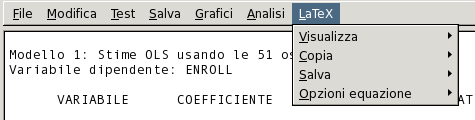
\includegraphics[scale=0.75]{figures/latex_menu}
  \end{center}
\end{figure}

The first three sub-items have branches titled ``Tabular'' and
``Equation''.  By ``Tabular'' we mean that the model is represented in
the form of a table; this is the fullest and most explicit
presentation of the results.  See Table~\ref{tab:mod1} for an example;
this was pasted into the manual after using the ``Copy, Tabular'' item
in \app{gretl} (a few lines were edited out for brevity).

\begin{table}[htbp]
\caption{Example of \LaTeX\ tabular output}
\label{tab:mod1}
\begin{center}

Model 1: OLS estimates using the 51 observations 1--51\\
Dependent variable: ENROLL\\

\vspace{1em}

\begin{tabular*}{.8\textwidth}{@{\extracolsep{\fill}}
l% col 1: varname
  D{.}{.}{-1}% col 2: coeff
    D{.}{.}{-1}% col 3: sderr
      D{.}{.}{-1}% col 4: t-stat
        D{.}{.}{4}}% col 5: p-value (or slope)
Variable &
  \multicolumn{1}{c}{Coefficient} &
    \multicolumn{1}{c}{Std.\ Error} &
      \multicolumn{1}{c}{$t$-statistic} &
        \multicolumn{1}{c}{p-value} \\[1ex]
const &
  0.241105 &
    0.0660225 &
      3.6519 &
        0.0007 \\
CATHOL &
  0.223530 &
    0.0459701 &
      4.8625 &
        0.0000 \\
PUPIL &
  -0.00338200 &
    0.00271962 &
      -1.2436 &
        0.2198 \\
WHITE &
  -0.152643 &
    0.0407064 &
      -3.7499 &
        0.0005 \\
\end{tabular*}

\vspace{1em}

\begin{tabular}{lD{.}{.}{-1}}
Mean of dependent variable & 0.0955686 \\
 S.D. of dependent variable & 0.0522150 \\
Sum of squared residuals & 0.0709594 \\
Standard error of residuals ($\hat{\sigma}$) & 0.0388558 \\
Unadjusted $R^2$ & 0.479466 \\
Adjusted $\bar{R}^2$ & 0.446241 \\
$F(3, 47)$ & 14.4306 \\
\end{tabular}
\end{center}
\end{table}

The ``Equation'' option is fairly self-explanatory --- the results are
written across the page in equation format, as below:

%%% the following needs the amsmath LaTeX package

\begin{gather}
\widehat{\rm ENROLL} = 
\underset{(0.066022)}{0.241105}
+\underset{(0.04597)}{0.223530}\,\mbox{CATHOL}
-\underset{(0.0027196)}{0.00338200}\,\mbox{PUPIL}
-\underset{(0.040706)}{0.152643}\,\mbox{WHITE}
 \notag \\
T = 51 \quad \bar{R}^2 = 0.4462 \quad F(3,47) = 14.431 \quad \hat{\sigma} = 0.038856\notag \\
\centerline{(standard errors in parentheses)} \notag
\end{gather}

The distinction between the ``Copy'' and ``Save'' options (for both
tabular and equation) is twofold.  First, ``Copy'' puts the \TeX\
source on the clipboard while with ``Save'' you are prompted for the
name of a file into which the source should be saved.  Second, with
``Copy'' the material is copied as a ``fragment'' while with ``Save''
it is written as a complete file.  The point is that a well-formed
\TeX\ source file must have a header that defines the
\texttt{documentclass} (article, report, book or whatever) and tags
that say \verb|\begin{document}| and \verb|\end{document}|.  This
material is included when you do ``Save'' but not when you do
``Copy'', since in the latter case the expectation is that you will
paste the data into an existing \TeX\ source file that already has the
relevant apparatus in place.

The items under ``Equation options'' should be self-explanatory: when
printing the model in equation form, do you want standard errors or
$t$-ratios displayed in parentheses under the parameter estimates?
The default is to show standard errors; if you want $t$-ratios, select
that item.  

\subsection{Other windows}

Several other sorts of output windows also have \TeX\ preview, copy
and save enabled.  In the case of windows having a graphical toolbar,
look for the \TeX\ button.  Figure~\ref{fig:tex-icon} shows this icon
(second from the right on the toolbar) along with the dialog that
appears when you press the button.

\begin{figure}[htbp]
  \caption{\TeX\ icon and dialog}
  \label{fig:tex-icon}
    \begin{center}
      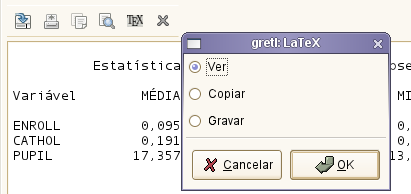
\includegraphics[scale=0.75]{figures/texdialog} 
    \end{center}
\end{figure}

One aspect of \app{gretl}'s \TeX\ support that is likely to be
particularly useful for publication purposes is the ability to produce
a typeset version of the ``model table'' (see
section~\ref{model-table}).  An example of this is shown in
Table~\ref{tab:modeltab}.

\begin{table}[htbp]
\caption{Example of model table output}
\label{tab:modeltab}
\begin{center}
OLS estimates\\
Dependent variable: ENROLL \\
\vspace{1em}

\begin{tabular}{lccc}
 & Model 1  & Model 2  & Model 3 \\  [6pt] 
const & $\,\,$0.2907$^{**}$ & $\,\,$0.2411$^{**}$ & 0.08557 \\
& \footnotesize{(0.07853)} & \footnotesize{(0.06602)} & \footnotesize{(0.05794)} \\ [4pt] 
CATHOL & $\,\,$0.2216$^{**}$ & $\,\,$0.2235$^{**}$ & $\,\,$0.2065$^{**}$ \\
& \footnotesize{(0.04584)} & \footnotesize{(0.04597)} & \footnotesize{(0.05160)} \\ [4pt] 
PUPIL & $-$0.003035 & $-$0.003382 & $-$0.001697 \\
& \footnotesize{(0.002727)} & \footnotesize{(0.002720)} & \footnotesize{(0.003025)} \\ [4pt] 
WHITE & $\,\,$$-$0.1482$^{**}$ & $\,\,$$-$0.1526$^{**}$ & \\
& \footnotesize{(0.04074)} & \footnotesize{(0.04071)} & \\ [4pt] 
ADMEXP & $-$0.1551 & & \\
& \footnotesize{(0.1342)} & & \\ [4pt] 
$n$ & 51 & 51 & 51 \\
$\bar R^2$ & 0.4502 & 0.4462 & 0.2956 \\
$\ell$ & 96.09 & 95.36 & 88.69 \\
\end{tabular}

\vspace{1em}
Standard errors in parentheses\\
{}* indicates significance at the 10 percent level\\
{}** indicates significance at the 5 percent level\\
\end{center}
\end{table}


\section{Fine-tuning typeset output}
\label{tex-tune}

There are three aspects to this: adjusting the appearance of the
output produced by \app{gretl} in \LaTeX\ preview mode; adjusting the
formatting of \app{gretl}'s tabular output for models when using the
\texttt{tabprint} command; and incorporating \app{gretl}'s output into
your own \TeX\ files.


\subsection{Previewing in the GUI}

As regards \emph{preview mode}, you can control the appearance of
\app{gretl}'s output using a file named \verb+gretlpre.tex+, which
should be placed in your \app{gretl} user directory (see the \GCR).
If such a file is found, its contents will be used as the ``preamble''
to the \TeX\ source.  The default value of the preamble is as follows:
    
\begin{code}
\documentclass[11pt]{article}
\usepackage[latin1]{inputenc} %% but see below
\usepackage{amsmath}
\usepackage{dcolumn,longtable}
\begin{document}
\thispagestyle{empty}
\end{code}

Note that the \verb+amsmath+ and \verb+dcolumn+ packages are required.
(For some sorts of output the \verb+longtable+ package is also
needed.)  Beyond that you can, for instance, change the type size or
the font by altering the \texttt{documentclass} declaration or
including an alternative font package.

The line \verb|\usepackage[latin1]{inputenc}| is automatically
changed if \app{gretl} finds itself running on a system where UTF-8
is the default character encoding --- see section~\ref{tex-encode}
below.

In addition, if you should wish to typeset \app{gretl} output in more
than one language, you can set up per-language preamble files.  A
``localized'' preamble file is identified by a name of the form
\verb|gretlpre_xx.tex|, where \texttt{xx} is replaced by the first two
letters of the current setting of the \texttt{LANG} environment
variable.  For example, if you are running the program in Polish,
using \verb|LANG=pl_PL|, then \app{gretl} will do the following when
writing the preamble for a \TeX\ source file.

\begin{enumerate}
\item Look for a file named \verb|gretlpre_pl.tex| in the \app{gretl}
  user directory.  If this is not found, then
\item look for a file named \verb|gretlpre.tex| in the \app{gretl}
  user directory.  If this is not found, then
\item use the default preamble.
\end{enumerate}

Conversely, suppose you usually run \app{gretl} in a language other
than English, and have a suitable \verb|gretlpre.tex| file in place
for your native language.  If on some occasions you want to produce
\TeX\ output in English, then you could create an additional
file \verb|gretlpre_en.tex|: this file will be used for the preamble
when \app{gretl} is run with a language setting of, say,
\verb|en_US|.  


\subsection{Command-line options}

After estimating a model via a script --- or interactively via the
\app{gretl} console or using the command-line program \app{gretlcli}
--- you can use the commands \texttt{tabprint} or \texttt{eqnprint} to
print the model to file in tabular format or equation format
respectively.  These options are explained in the \GCR{}.  

If you wish alter the appearance of \app{gretl}'s tabular output for
models in the context of the \texttt{tabprint} command, you can
specify a custom row format using the \option{format} flag.  The
format string must be enclosed in double quotes and must be tied to
the flag with an equals sign.  The pattern for the format string is as
follows.  There are four fields, representing the coefficient,
standard error, $t$-ratio and p-value respectively.  These fields
should be separated by vertical bars; they may contain a
\texttt{printf}-type specification for the formatting of the numeric
value in question, or may be left blank to suppress the printing of
that column (subject to the constraint that you can't leave all the
columns blank).  Here are a few examples:

\begin{code}
--format="%.4f|%.4f|%.4f|%.4f"
--format="%.4f|%.4f|%.3f|"
--format="%.5f|%.4f||%.4f"
--format="%.8g|%.8g||%.4f"
\end{code}

The first of these specifications prints the values in all columns
using 4 decimal places.  The second suppresses the p-value and prints
the $t$-ratio to 3 places.  The third omits the $t$-ratio.  The last
one again omits the $t$, and prints both coefficient and standard
error to 8 significant figures.

Once you set a custom format in this way, it is remembered and used
for the duration of the gretl session.  To revert to the default
formatting you can use the special variant \verb|--format=default|.


\subsection{Further editing}

Once you have pasted \app{gretl}'s \TeX\ output into your own
document, or saved it to file and opened it in an editor, you can of
course modify the material in any wish you wish.  In some cases,
machine-generated \TeX\ is hard to understand, but \app{gretl}'s
output is intended to be human-readable and -editable.  In addition,
it does not use any non-standard style packages.  Besides the standard
\LaTeX\ document classes, the only files needed are, as noted above,
the \verb+amsmath+, \verb+dcolumn+ and \verb+longtable+ packages.
These should be included in any reasonably full \TeX\ implementation.


\section{Character encodings}
\label{tex-encode}

People using \app{gretl} in English-speaking locales are unlikely to
have a problem with this, but if you're generating \TeX\ output in a
locale where accented characters (not in the ASCII character set) are
employed, you may want to pay attention here.

\app{Gretl} generates \TeX\ output using whatever character encoding
is standard on the local system.  If the system encoding is in the
ISO-8859 family, this will probably be OK wihout any special effort on
the part of the user.  Newer GNU/Linux systems, however, typically use
Unicode (UTF-8).  This is also OK so long as your \TeX\ system can
handle UTF-8 input, which requires use of the \app{latex-ucs} package.
So: if you are using \app{gretl} to generate \TeX\ in a non-English
locale, where the system encoding is UTF-8, you will need to ensure
that the \app{latex-ucs} package is installed.  This package may or
may not be installed by default when you install \TeX{}.

For reference, if \app{gretl} detects a UTF-8 environment, the
following lines are used in the \TeX\ preamble:
%
\begin{code}
\usepackage{ucs}
\usepackage[utf8x]{inputenc}
\end{code}


\section{Installing and learning \TeX}
\label{tex-install}

This is not the place for a detailed exposition of these matters, but
here are a few pointers.  

So far as we know, every GNU/Linux distribution has a package or set
of packages for \TeX, and in fact these are likely to be installed by
default.  Check the documentation for your distribution.  For MS
Windows, several packaged versions of \TeX\ are available: one of the
most popular is MiK\TeX\, at \url{http://www.miktex.org/}.  For Mac OS
X a nice implementation is i\TeX{}Mac, at
\url{http://itexmac.sourceforge.net/}.  An essential starting point for
online \TeX\ resources is the Comprehensive
\TeX\ Archive Network (CTAN) at \url{http://www.ctan.org/}.

As for learning \TeX, many useful resources are available both online
and in print.  Among online guides, Tony Roberts' ``\LaTeX: from quick
and dirty to style and finesse'' is very helpful, at

\url{http://www.sci.usq.edu.au/staff/robertsa/LaTeX/latexintro.html}

An excellent source for advanced material is \emph{The \LaTeX\
  Companion} (Goossens \textit{et al.}, 2004).


%%% Local Variables: 
%%% mode: latex
%%% TeX-master: "gretl-guide"
%%% End: 

\chapter{Troubleshooting gretl}
\label{trouble}

\section{Bug reports}
\label{trouble-bugs}

Bug reports are welcome. Hopefully, you are unlikely to find bugs in
the actual calculations done by \app{gretl} (although this statement
does not constitute any sort of warranty). You may, however, come
across bugs or oddities in the behavior of the graphical interface.
Please remember that the usefulness of bug reports is greatly enhanced
if you can be as specific as possible: what \emph{exactly} went wrong,
under what conditions, and on what operating system?  If you saw an
error message, what precisely did it say?

\section{Auxiliary programs}
\label{trouble-programs}

As mentioned above, \app{gretl} calls some other programs to
accomplish certain tasks (gnuplot for graphing, {\LaTeX} for
high-quality typesetting of regression output, GNU R).  If something
goes wrong with such external links, it is not always easy for
\app{gretl} to produce an informative error message.  If such a link
fails when accessed from the \app{gretl} graphical interface, you may
be able to get more information by starting \app{gretl} from the
command prompt rather than via a desktop menu entry or icon.  On the X
window system, start gretl from the shell prompt in an \app{xterm}; on
MS Windows, start the program \cmd{gretlw32.exe} from a console
window or ``DOS box''.  Additional error messages may be displayed on
the terminal window.

Also please note that for most external calls, \app{gretl} assumes
that the programs in question are available in your ``path'' --- that
is, that they can be invoked simply via the name of the program,
without supplying the program's full location.\footnote{The exception
  to this rule is the invocation of gnuplot under MS Windows, where a
  full path to the program is given.}  Thus if a given program fails,
try the experiment of typing the program name at the command prompt,
as shown below.

\begin{center}
  \begin{tabular}{llll}
    & \textit{Graphing} & \textit{Typesetting} & \textit{GNU R}\\
    X window system & gnuplot & latex, xdvi & R\\
    MS Windows & wgnuplot.exe & pdflatex & RGui.exe\\
  \end{tabular}
\end{center}

If the program fails to start from the prompt, it's not a \app{gretl}
issue but rather that the program's home directory is not in your
path, or the program is not installed (properly).  For details on
modifying your path please see the documentation or online help for
your operating system or shell.
    
%%% Local Variables: 
%%% mode: latex
%%% TeX-master: "gretl-guide"
%%% End: 


\chapter{L'interfaccia a riga di comando}
\label{cli}



\section{Gretl sul terminale}
\label{cli-console}


Il pacchetto \app{gretl} include il programma a riga di comando
\app{gretlcli}. Su Linux � possibile esegurlo in un terminale testuale
o in un xterm (o simili), mentre su MS Windows pu� essere eseguito in
una finestra di terminale (quella che di solito viene chiamata
``prompt di MS-DOS'').  \app{gretlcli} ha un file di aiuto, a cui si
accede inserendo il comando ``help'' al prompt. Inoltre, pu� essere
usato in modalit� batch, inviando i risultati direttamente a un file
(si veda XXX).
    
Se \app{gretlcli} � linkato alla libreria \app{readline} (ci� avviene
automaticamente nella versione MS Windows, si veda anche l'[?]), �
possibile richiamare e modificare i comandi gi� eseguiti, inoltre �
disponibile il completamento automatico dei comandi. Per muoversi
nella lista dei comandi gi� eseguiti � possibile usare i tasti Freccia
Su/Gi�, mentre per muoversi sulla riga di comando � possibile usare i
tasti Freccia a destra/sinistra e le scorciatoie in stile
Emacs\footnote{In realt� quelli mostrati sono i valori predefiniti, ma
  possono essere modificati: si veda il
  \href{http://cnswww.cns.cwru.edu/~chet/readline/readline.html}{manuale
    di readline}.}. Le scorciatoie pi� usate sono:
    

\begin{center}
  \begin{tabular}{ll}
    Scorciatoia & Effetto\\
    \verb+Ctrl-a+ & Va all'inizio della riga\\
    \verb+Ctrl-e+ & Va alla fine della riga\\
    \verb+Ctrl-d+ & Cancella il carattere a destra\\
  \end{tabular}
\end{center}


dove ``\verb+Ctrl-a+'' significa premere il tasto ``\verb+a+'' mentre
si tiene premuto il tasto ``\verb+Ctrl+''.  Quindi se si vuole
correggere qualcosa all'inizio della riga di comando, \emph{non
  occorre} usare il tasto di cancellazione all'indietro su tutta la
riga, basta saltare all'inizio della riga e aggiungere o cancellare i
caratteri desiderati.  Inserendo le prime lettere del nome di un
comando e premendo il tasto Tab, readline cercher� di completare
automaticamente il nome del comando. Se esiste un solo modo di
completare le lettere inserite, verr� inserito il comando
corrispondente, altrimenti premendo Tab una seconda volta verr�
visualizzata una lista delle alternative possibili.
    

\section{Differenze con ESL di Ramanathan}
\label{cli-syntax}

\app{gretlcli} ha ereditato la sintassi di base dei comandi dal
programma \app{ESL} di Ramu Ramanathan e gli script di comandi
sviluppati per \app{ESL} dovrebbero essere utilizzabili con con pochi
cambiamenti: le uniche cose a cui stare attenti sono i comandi
multilinea e il comando \cmd{freq}.
    
\begin{itemize}
\item In \app{ESL} viene usato un punto e virgola come terminatore per
  molti comandi.  In \app{gretlcli} ho deciso di rimuovere questa
  caratteristica: il carattere punto e virgola � semplicemente
  ignorato, a parte in alcuni casi speciali in cui ha un significato
  particolare: come separatore per due liste nei comandi \cmd{ar} e
  \cmd{tsls}, e come segnaposto per l'osservazione iniziale o finale
  immutata nel comando \cmd{smpl}. In \app{ESL} il punto e virgola d�
  la possibilit� di spezzare le righe di comando su pi� righe dello
  schermo; in \app{gretlcli} si ottiene questo risultato inserendo una
  barra rovesciata \verb+\+ alla fine della riga da spezzare.
	
\item Per quanto riguarda \cmd{freq}, al momento non � possibile
  specificare intervalli personalizzati, come avviene in \app{ESL}.
  Inoltre, ai risultati del comando � stato aggiunto un test
  chi-quadro di normalit�.
	
\end{itemize}


Si noti anche che i comandi per usare la modalit� batch sono stati
semplificati. In \app{ESL} si usava, ad esempio:
      
\begin{verbatim}
        esl -b filedati < fileinput > fileoutput
\end{verbatim}

mentre in \app{gretlcli} si usa:
      
\begin{verbatim}
	gretlcli -b fileinput > fileoutput
\end{verbatim}


Il file di input viene trattato come un argomento del programma,
mentre il file di dati su cui operare va indicato all'interno del file
di input, usando il comando \cmd{open datafile} o il commento speciale
\verb+(* !+ filedati \verb+*)+.
    
%%% Local Variables: 
%%% mode: latex
%%% TeX-master: "gretl-guide-it"
%%% End: 



\begin{appendices}
\chapter{Data file details}
\label{app-datafile}

\section{Basic native format}
\label{native}

In \app{gretl}'s native data format, a data set is stored in XML
(extensible mark-up language). Data files correspond to the simple DTD
(document type definition) given in \verb+gretldata.dtd+, which is
supplied with the \app{gretl} distribution and is installed in the
system data directory (e.g.\ \url{/usr/share/gretl/data} on Linux.)
Data files may be plain text or gzipped.  They contain the actual data
values plus additional information such as the names and descriptions
of variables, the frequency of the data, and so on.

Most users will probably not have need to read or write such files
other than via \app{gretl} itself, but if you want to manipulate them
using other software tools you should examine the DTD and also take a
look at a few of the supplied practice data files: \verb+data4-1.gdt+
gives a simple example; \verb+data4-10.gdt+ is an example where
observation labels are included.

\section{Traditional ESL format}
\label{traddata}

For backward compatibility, \app{gretl} can also handle data files in
the ``traditional'' format inherited from Ramu Ramanathan's \app{ESL}
program.  In this format a data set is represented by two text files;
one contains the actual data and the other information on how the data
should be read.  To be more specific:

\begin{enumerate}
\item \emph{Actual data}: A rectangular matrix of white-space
  separated numbers. By default, each column represents a variable,
  each row an observation. The data columns can be separated by spaces
  or tabs. Traditionally the data filename has no extension/suffix.
\item \emph{Header}: The data file must be accompanied by a header
  file which has the same basename as the data file plus the suffix
  \verb+.hdr+.  This file contains, in order:
  \begin{itemize}
  \item (Optional) \emph{comments} on the data, set off by the opening
    string \verb+(*+ and the closing string \verb+*)+, each of these
    strings to occur on lines by themselves.
  \item (Required) a list of the \emph{names of the variables} in the
    data file, separated by white space. Names are limited to 8
    characters, must start with a letter, and are limited to
    alphanumeric characters plus the underscore.  The list may
    continue over more than one line; it should be terminated with a
    semicolon.
  \item (Required) an \emph{observations} line of the form
    \verb+1 1 85+.  The first element gives the data frequency (1 for
    undated or annual data, 4 for quarterly, 12 for monthly).  The
    second and third elements give the starting and ending
    observations.  These should be 1 and the number of observations,
    respectively, for undated data.  For time-series data one can use
    dates of the form \cmd{1959.1} (quarterly, one digit after the
    point) or \cmd{1967.03} (monthly, two digits after the point).
  \item The keyword \verb+BYOBS+ (but see below).
  \end{itemize}
\end{enumerate}

Here is an example of a well-formed data header file; the
corresponding data file contains three columns of data, each having 90
entries.

\begin{code} 
(* 
  DATA9-6: 
  Data on log(money), log(income) and interest rate from US. 
  Source: Stock and Watson (1993) Econometrica 
  (unsmoothed data) Period is 1900-1989 (annual data). 
  Data compiled by Graham Elliott. 
*) 
lmoney lincome intrate ; 
1 1900 1989 BYOBS
\end{code}

Three further features of the traditional ESL data format may be
noted.
    
\begin{enumerate}
\item If the \verb+BYOBS+ keyword is replaced by \verb+BYVAR+ this
  indicates that in the corresponding data file the data are written
  out by variable rather than by observation.
\item If \verb+BYOBS+ is followed by the keyword \verb+MARKERS+,
  \app{gretl} expects a data file in which the \emph{first column}
  contains strings (8 characters maximum) used to identify the
  observations.  This may be useful in the case of cross-sectional data
  where the units of observation are identifiable: countries, states,
  cities or whatever.  It can also be useful for irregular time series
  data, such as daily stock price data where some days are not trading
  days --- in this case the observations can be marked with a date
  string such as \cmd{10/01/98}.  (Remember the 8-character maximum.)
  Note that \cmd{BYVAR} and \cmd{MARKERS} are mutually exclusive
  flags.  Also note that the ``markers'' are not considered to be a
  variable: this column does not have a corresponding entry in the
  list of variable names in the header file.
\item If a file with the same base name as the data file and header
  files, but with the suffix \verb+.lbl+, is found, it is read to fill
  out the descriptive labels for the data series. The format of the
  label file is simple: each line contains the name of one variable
  (as found in the header file), followed by one or more spaces,
  followed by the descriptive label. Here is an example, giving
  a label for a variable named ``price'':
  \verb+price New car price index, 1982 base year+
\end{enumerate}

If you want to save data in traditional format, use the
\verb|--traditional| flag with the \cmd{store} command, either in the
command-line program or in the console window of the GUI program.


\section{Binary database details}
\label{dbdetails}

A \app{gretl} database consists of two parts: an ASCII index file
(with filename suffix \verb+.idx+) containing information on the
series, and a binary file (suffix \verb+.bin+) containing the actual
data.  Two examples of the format for an entry in the \verb+idx+ file
are shown below:

\begin{code}
G0M910  Composite index of 11 leading indicators (1987=100) 
M 1948.01 - 1995.11  n = 575
currbal Balance of Payments: Balance on Current Account; SA 
Q 1960.1 - 1999.4 n = 160
\end{code}

The first field is the series name.  The second is a description of
the series (maximum 128 characters).  On the second line the first
field is a frequency code: \verb+M+ for monthly, \verb+Q+ for
quarterly, \verb+A+ for annual, \verb+B+ for business-daily (daily
with five days per week) and \verb+D+ for daily (seven days per week).
No other frequencies are accepted at present.  Then comes the starting
date (N.B. with two digits following the point for monthly data, one
for quarterly data, none for annual), a space, a hyphen, another
space, the ending date, the string ``\verb+n = +'' and the integer
number of observations. In the case of daily data the starting and
ending dates should be given in the form \verb+YYYY/MM/DD+. This
format must be respected exactly.

Optionally, the first line of the index file may contain a short
comment (up to 64 characters) on the source and nature of the data,
following a hash mark.  For example:

\begin{code}
# Federal Reserve Board (interest rates)
\end{code}

The corresponding binary database file holds the data values,
represented as ``floats'', that is, single-precision floating-point
numbers, typically taking four bytes apiece.  The numbers are packed
``by variable'', so that the first \emph{n} numbers are the
observations of variable 1, the next \emph{m} the observations on
variable 2, and so on.

\chapter{Gretl and ODBC}
\label{chap:odbc}

Gretl provides a method for retrieving data from databases which
support the Open Database Connectivity (ODBC) standard. Most users
won't be interested in this, but there may be some for whom this
feature matters a lot---typically, those who work in an environment
where huge data collections are accessible via a Data Base Management
System (DBMS).

In the following section we explain what is needed for ODBC support in
gretl. We provide some background information on how ODBC works
in section~\ref{sec:odbc-base}, and explain the details of getting
gretl to retrieve data from a database in
section~\ref{sec:odbc-syntax}. Section~\ref{sec:odbc-examples}
provides some example of usage, and section~\ref{sec:odbc-conn} gives
some details on the management of ODBC connections.

\section{ODBC support}
\label{sec:odbc-support}

The piece of software that bridges between gretl and the ODBC system
is a dynamically loaded ``plugin''. This is included in the gretl
packages for MS Windows and Mac OS X. On other unix-type platforms
(notably Linux) you may have to build gretl from source to get ODBC
support.  This is because the plugin depends on having \app{unixODBC}
installed, which we cannot assume to be the case on typical Linux
systems. To enable the ODBC plugin when building gretl, you must pass
the option \verb|--with-odbc| to gretl's \texttt{configure} script. In
addition, if \app{unixODBC} is installed in a non-standard location
you will have to specify its installation prefix using
\verb|--with-ODBC-prefix|, as in (for example)
\begin{code}
  ./configure --with-odbc --with-ODBC-prefix=/opt/ODBC
\end{code}

\section{ODBC base concepts}
\label{sec:odbc-base}

ODBC is short for \emph{Open DataBase Connectivity}, a group of
software methods that enable a \emph{client} to interact with a
database \emph{server}. The most common operation is when the client
fetches some data from the server. ODBC acts as an intermediate layer
between client and server, so the client ``talks'' to ODBC rather than
accessing the server directly (see Figure~\ref{fig:odbc}).

\begin{figure}[htbp]
  \centering
  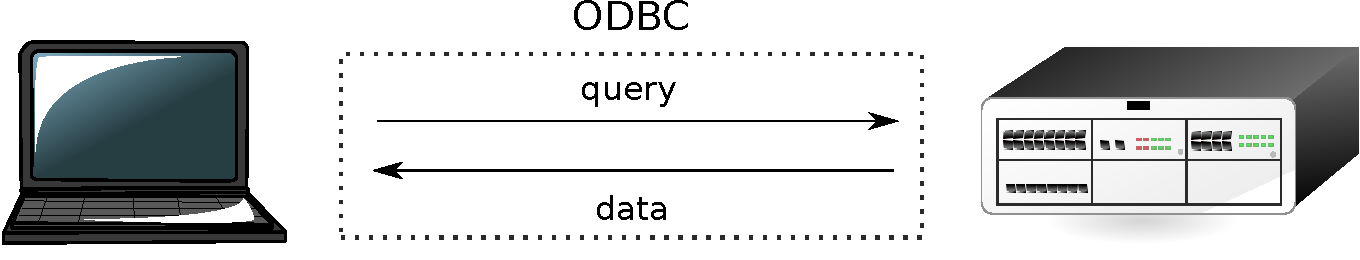
\includegraphics[width=0.8\textwidth]{figures/odbc}
  \caption{Retrieving data via ODBC}
  \label{fig:odbc}
\end{figure}

For the above mechanism to work, it is necessary that the relevant
ODBC software is installed and working on the client machine (contact
your DB administrator for details). At this point, the database (or
databases) that the server provides will be accessible to the client
as a \emph{data source} with a specific identifier (a Data Source Name
or DSN); in most cases, a username and a password are required to
connect to the data source.

Once the connection is established, the user sends a \emph{query} to
ODBC, which contacts the database manager, collects the results and
sends them back to the user. The query is almost invariably formulated
in a special language used for the purpose, namely SQL.\footnote{See
  \url{http://en.wikipedia.org/wiki/SQL}.} We will not provide here an
SQL tutorial: there are many such tutorials on the Net; besides, each
database manager tends to support its own SQL dialect so the precise
form of an SQL query may vary slightly if the DBMS on the other end is
Oracle, MySQL, PostgreSQL or something else.

Suffice it to say that the main statement for retrieving data is the
\texttt{SELECT} statement.  Within a DBMS, data are organized in
\emph{tables}, which are roughly equivalent to spreadsheets. The
\texttt{SELECT} statement returns a subset of a table, which is itself
a table. For example, imagine that the database holds a table called
``NatAccounts'', containing the data shown in
Table~\ref{tab:odbc-nataccounts}.

\begin{table}[htbp]
  \centering
  \begin{tabular}{rrrrr}
    \hline
    year	& qtr	& gdp	 & consump	& tradebal \\ 
    \hline
    1970	& 1	& 584763 & 344746.9	& $-$5891.01 \\ 
    1970	& 2	& 597746 & 350176.9	& $-$7068.71 \\ 
    1970	& 3	& 604270 & 355249.7	& $-$8379.27 \\ 
    1970	& 4	& 609706 & 361794.7	& $-$7917.61 \\ 
    1971	& 1	& 609597 & 362490	& $-$6274.3  \\ 
    1971	& 2	& 617002 & 368313.6	& $-$6658.76 \\ 
    1971	& 3	& 625536 & 372605	& $-$4795.89 \\ 
    1971	& 4	& 630047 & 377033.9	& $-$6498.13  
  \end{tabular}
  \caption{The ``NatAccounts'' table}
  \label{tab:odbc-nataccounts}
\end{table}

The SQL statement
\begin{code}
  SELECT qtr, tradebal, gdp FROM NatAccounts WHERE year=1970;
\end{code}
produces the subset of the original data shown in Table~\ref{tab:odbc-result}.

\begin{table}[htbp]
  \centering
  \begin{tabular}{rrrrr}
    \hline
    qtr	& tradebal & gdp    \\ 
    \hline
    1	& $-$5891.01 & 584763 \\ 
    2	& $-$7068.71 & 597746 \\ 
    3	& $-$8379.27 & 604270 \\ 
    4	& $-$7917.61 & 609706  
  \end{tabular}
  \caption{Result of a \texttt{SELECT} statement}
  \label{tab:odbc-result}
\end{table}

Gretl provides a mechanism for forwarding your query to the DBMS
via ODBC and including the results in your currently open dataset.

\section{Syntax}
\label{sec:odbc-syntax}

At present we do not offer a graphical interface for ODBC import; this
must be done via the command line interface. The two commands used for
fetching data via an ODBC connection are \texttt{open} and
\texttt{data}.

The \texttt{open} command is used for connecting to a DBMS: its syntax
is
\begin{flushleft}
\texttt{%
  open dsn=\emph{database} [user=\emph{username}]
  [password=\emph{password}]} \option{odbc}
\end{flushleft}
The \texttt{user} and \texttt{password} items are optional; the effect
of this command is to initiate an ODBC connection. It is assumed that
the machine gretl runs on has a working ODBC client installed.

In order to actually retrieve the data, the \texttt{data} command is
used. Its syntax is:
\begin{flushleft}
\texttt{%
  data \emph{series} [obs-format=\emph{format-string}] query=\emph{query-string}} \option{odbc}
\end{flushleft}
where:
\begin{description}
\item[\emph{series}] is a list of names of gretl series to contain the
  incoming data, separated by spaces.  Note that these series need not
  exist pior to the ODBC import.
\item[\emph{format-string}] is an optional parameter, used to handle
  cases when a ``rectangular'' organisation of the database cannot be
  assumed (more on this later);
\item[\emph{query-string}] is a string containing the SQL statement
  used to extract the data.
\end{description}
%
There should be no spaces around the equals signs in the
\texttt{obs-format} and \texttt{query} fields in the \texttt{data}
command.

The \texttt{\emph{query-string}} can, in principle, contain any valid
SQL statement which results in a table. This string may be specified
directly within the command, as in
\begin{code}
  data x query="SELECT foo FROM bar" --odbc
\end{code}
which will store into the gretl variable \texttt{x} the content of the
column \texttt{foo} from the table \texttt{bar}. However, since in a
real-life situation the string containing the SQL statement may be
rather long, it may be best to store it in a string variable.  For
example:
\begin{code}
  string SqlQry = "SELECT foo1, foo2 FROM bar"
  data x y query=SqlQry --odbc
\end{code}

\subsection{The observation format specifier}

If the optional parameter \texttt{obs-format} is absent, as in the
above example, the SQL query should return $k$ columns of data, where
$k$ is the number of series names listed in the \texttt{data} command.
It may be necessary to include a \texttt{smpl} command before the
\texttt{data} command to set up the right ``window'' for the incoming
data.  In addition, if one cannot assume that the data will be
delivered in the correct order (typically, chronological order), the
SQL query should contain an appropriate \texttt{ORDER BY} clause.

The optional format string is used for those cases when there is no
certainty that the data from the query will arrive in the same order
as the gretl dataset. This may happen when missing values are
interspersed within a column, or with data that do not have a natural
ordering, e.g.\ cross-sectional data. In this case, the SQL statement
should return a table with $m+k$ columns, where the first $m$
columns are used to identify the observation or row in the gretl
dataset into which the actual data values in the final $k$ columns
should be placed.  The \texttt{obs-format} string is used to translate
the first $m$ fields into a string which matches the string
gretl uses to identify observations in the currently open
dataset. Up to three columns can be used for this purpose ($m \leq
3$).

Note that the strings gretl uses to identify observations
can be seen by printing any variable ``by observation'', as in
%
\begin{code}
print index --byobs
\end{code}
%
(The series named \texttt{index} is automatically added to a dataset
created via the \texttt{nulldata} command.)

The format specifiers available for use with \texttt{obs-format} are
as follows:

\begin{center}
\begin{tabular}{ll}
\texttt{\%d} & print an integer value \\
\texttt{\%s} & print an string value \\
\texttt{\%g} & print a floating-point value \\
\end{tabular}
\end{center}

In addition the format can include literal characters to be passed
through, such as slashes or colons, to make the resulting string
compatible with gretl's observation identifiers.

For example, consider the following fictitious case: we have a
5-days-per-week dataset, to which we want to add the stock index for
the Verdurian market;\footnote{See
  \url{http://www.almeopedia.com/index.php/Verduria}.} it so
happens that in Verduria Saturdays are working days but Wednesdays are
not. We want a column which does \emph{not} contain data on
Saturdays, because we wouldn't know where to put them, but at the same
time we want to place missing values on all the Wednesdays.

In this case, the following syntax could be used
%
\begin{code}
  string QRY="SELECT year,month,day,VerdSE FROM AlmeaIndexes"
  data y obs-format="%d-%d-%d" query=QRY --odbc
\end{code}
%
The column \texttt{VerdSE} holds the data to be fetched, which will go
into the gretl series \texttt{y}. The first three columns are
used to construct a string which identifies the day. Daily dates take
the form \texttt{YYYY-MM-DD} in gretl.  If a row from the DBMS
produces the observation string \texttt{2008-04-01} this will match OK
(it's a Tuesday), but \texttt{2008-04-05} will not match since it is a
Saturday; the corresponding row will therefore be discarded.  On the
other hand, since no string \texttt{2008-04-23} will be found in the
data coming from the DBMS (it's a Wednesday), that entry is left blank
in our series \texttt{y}.

\section{Examples}
\label{sec:odbc-examples}

\begin{table}[htbp]
  \centering
  \begin{tabular}{p{0.4\textwidth}p{0.4\textwidth}}
  Table \texttt{Consump} &
  Table \texttt{DATA} \\
    
\begin{tabular}{ll}
\hline
 Field   & Type           \\ 
\hline 
 time    & decimal(7,2)   \\ 
 income  & decimal(16,6) \\ 
 consump & decimal(16,6) \\
\hline
\end{tabular} &

\begin{tabular}{ll}
\hline
 Field   & Type           \\ 
\hline 
 year    & decimal(4,0)  \\ 
 qtr     & decimal(1,0)  \\ 
 varname & varchar(16)   \\ 
 xval    & decimal(20,10)\\ 
\hline
\end{tabular}

  \end{tabular}

  \caption{Example AWM database -- structure}
  \label{tab:odbc-AWMexample1}
\end{table}

\begin{table}[htbp]
  \centering
  \begin{tabular}{p{0.475\textwidth}p{0.475\textwidth}}
  Table \texttt{Consump} &
  Table \texttt{DATA} \\
    
\begin{tabular}{lll}
  1970.00	& 424278.975500	& 344746.944000 \\ 
  1970.25	& 433218.709400	& 350176.890400 \\ 
  1970.50	& 440954.219100	& 355249.672300 \\ 
  1970.75	& 446278.664700	& 361794.719900 \\ 
  1971.00	& 447752.681800	& 362489.970500 \\ 
  1971.25	& 453553.860100	& 368313.558500 \\ 
  1971.50	& 460115.133100	& 372605.015300 \\ 
\ldots \\ 
\end{tabular} &

\begin{tabular}{lllr}
1970	& 1	& CAN	& $-$517.9085000000\\ 
1970	& 2	& CAN	& 662.5996000000 \\ 
1970	& 3	& CAN	& 1130.4155000000\\ 
1970	& 4	& CAN	& 467.2508000000 \\ 
1970	& 1	& COMPR	& 18.4000000000  \\ 
1970	& 2	& COMPR	& 18.6341000000  \\ 
1970	& 3	& COMPR	& 18.3000000000  \\ 
1970	& 4	& COMPR	& 18.2663000000  \\ 
1970	& 1	& D1	& 1.0000000000   \\ 
1970	& 2	& D1	& 0.0000000000   \\ 
\ldots \\ 
\end{tabular}
\end{tabular}
  \caption{Example AWM database --- data}
  \label{tab:odbc-AWMexample2}
\end{table}

In the following examples, we will assume that access is available to
a database known to ODBC with the data source name ``AWM'', with
username ``Otto'' and password ``Bingo''. The database ``AWM''
contains quarterly data in two tables (see \ref{tab:odbc-AWMexample1}
and \ref{tab:odbc-AWMexample2}):

The table \texttt{Consump} is the classic ``rectangular'' dataset;
that is, its internal organization is the same as in a spreadsheet or
econometrics package: each row is a data point and each column is a
variable. The structure of the \texttt{DATA} table
is different: each record is one figure, stored in the column
\texttt{xval}, and the other fields keep track of which variable it
belongs to, for which date.

\begin{script}[htbp]
  \fragcaption{Simple query from a rectangular table}
  \label{ex:odbc-1}
\begin{scode}
nulldata 160
setobs 4 1970:1 --time
open dsn=AWM user=Otto password=Bingo --odbc

string Qry = "SELECT consump, income FROM Consump"
data cons inc query=Qry --odbc
\end{scode}
\end{script}

Listing~\ref{ex:odbc-1} shows a query for two series: first we set up
an empty quarterly dataset. Then we connect to the database using the
\texttt{open} statement. Once the connection is established we
retrieve two columns from the \texttt{Consump} table. No observation
string is required because the data already have a suitable structure;
we need only import the relevant columns.

\begin{script}[htbp]
  \caption{Simple query from a non-rectangular table}
  \label{ex:odbc-2}
\begin{scode}
string S = "select year, qtr, xval from DATA \
       where varname='WLN' ORDER BY year, qtr"
data wln obs-format="%d:%d" query=S --odbc
\end{scode}
\end{script}

In example~\ref{ex:odbc-2}, by contrast, we make use of the
observation string since we are drawing from the \texttt{DATA}
table, which is not rectangular. The SQL statement stored in the
string \texttt{S} produces a table with three columns. The
\texttt{ORDER BY} clause ensures that the rows will be in
chronological order, although this is not strictly necessary in this
case.

\begin{script}[htbp]
  \caption{Handling of missing values for a non-rectangular table}
  \label{ex:odbc-3}
\begin{scode}
string foo = "select year, qtr, xval from DATA \
       where varname='STN' AND qtr>1"
data bar obs-format="%d:%d" query=foo --odbc
print bar --byobs
\end{scode}

Listing \ref{ex:odbc-3} shows what happens if the rows in
the outcome from the \texttt{SELECT} statement do not match the
observations in the currently open gretl dataset. The query
includes a condition which filters out all the data from the first
quarter. The query result (invisible to the user) would be something
like
\begin{code}
+------+------+---------------+
| year | qtr  | xval          |
+------+------+---------------+
| 1970 |    2 |  7.8705000000 | 
| 1970 |    3 |  7.5600000000 | 
| 1970 |    4 |  7.1892000000 | 
| 1971 |    2 |  5.8679000000 | 
| 1971 |    3 |  6.2442000000 | 
| 1971 |    4 |  5.9811000000 | 
| 1972 |    2 |  4.6883000000 | 
| 1972 |    3 |  4.6302000000 | 
...
\end{code}
Internally, gretl fills the variable \texttt{bar} with the
corresponding value if it finds a match; otherwise, \texttt{NA} is
used. Printing out the variable \texttt{bar} thus produces
\begin{code}
     Obs           bar

  1970:1              
  1970:2        7.8705
  1970:3        7.5600
  1970:4        7.1892
  1971:1              
  1971:2        5.8679
  1971:3        6.2442
  1971:4        5.9811
  1972:1              
  1972:2        4.6883
  1972:3        4.6302
...
\end{code}

\end{script}

\section{Connectivity details}
\label{sec:odbc-conn}

It may be helpful to supply some details on gretl's management of ODBC
connections. First, when the \cmd{open} command is invoked with the
\option{odbc} option, gretl checks to see if a connection to the
specified DSN (Data Source Name) can be established via the ODBC
function \texttt{SQLConnect}. If not, an error is flagged; if so, the
connection is dropped (\texttt{SQLDisconnect}) but the DSN details are
stored. The stored DSN then remains the implicit source for subsequent
invocation of the \cmd{data} command, with the \option{odbc} option,
until a countermanding \cmd{open} command is issued.

Each time an OBDC-related \cmd{data} command is issued, gretl attempts
to re-establish a connection to the given DSN; the connection is
dropped once the data transfer is complete.

%%% Local Variables:
%%% mode: latex
%%% TeX-master: "gretl-guide"
%%% End:


\chapter{Building \app{gretl}: a step-by-step guide}
\label{app-build}

Here we give instructions detailed enough to allow a user
with only a basic knowledge of a Unix-type system to build \app{gretl}.
These steps were tested on a fresh installation of Debian Etch. For
other Linux distributions (especially Debian-based ones, like Ubuntu
and its derivatives) little should change. Other Unix-like operating
systems such as MacOSX and BSD would probably require more substantial
adjustments.

In this guided example, we will build \app{gretl} complete with
documentation.  This introduces a few more requirements, but gives you
the ability to modify the documentation files as well, like the help
files or the manuals.

\section{Installing the prerequisites}

We assume that the basic GNU utilities are already installed on the
system, together with these other programs:
\begin{itemize}
\item some \TeX/\LaTeX system (\texttt{texlive} will do beautifully)
\item Gnuplot
\item ImageMagick
\end{itemize}
We also assume that the user has administrative privileges and knows
how to install packages.  The examples below are carried out using the
\texttt{apt-get} shell command, but they can be performed with
menu-based utilities like \texttt{aptitude}, \texttt{dselect} or the
GUI-based program \texttt{synaptic}. Users of Linux distributions
which employ rpm packages (e.g.\ Red Hat/Fedora, Mandriva, SuSE) may
want to refer to the
\href{http://gretl.sourceforge.net/depend.html}{dependencies} page on
the \app{gretl} website.

The first step is installing the C compiler and related basic
utilities, if these are not already in place. On a Debian system,
these are contained in a bunch of packages that can be installed via
the command
\begin{code}
apt-get install gcc autoconf automake1.9 libtool flex bison gcc-doc \
libc6-dev libc-dev gfortran gettext pkgconfig
\end{code}

Then it is necessary to install the ``development'' (\texttt{dev})
packages for the libraries that \app{gretl} uses:
\begin{center}
  \begin{tabular}{ll}
    \textit{Library} & \textit{command} \\ [4pt]
    GLIB     & \texttt{apt-get install libglib2.0-dev} \\
    GTK 2.0  & \texttt{apt-get install libgtk2.0-dev} \\
    PNG      & \texttt{apt-get install libpng12-dev} \\
    XSLT     & \texttt{apt-get install libxslt1-dev} \\
    LAPACK   & \texttt{apt-get install liblapack-dev} \\
    FFTW     & \texttt{apt-get install libfftw3-dev} \\
    READLINE & \texttt{apt-get install libreadline-dev} \\
    ZLIB     & \texttt{apt-get install zlib1g-dev} \\
    XML      & \texttt{apt-get install libxml2-dev} \\
    GMP      & \texttt{apt-get install libgmp3-dev} \\
    CURL     & \texttt{apt-get install libcurl-dev} \\
    MPFR     & \texttt{apt-get install libmpfr-dev}
  \end{tabular}
\end{center}

(MPFR is optional, but recommended.)  The \texttt{dev} packages for
these libraries are necessary to \emph{compile} \app{gretl} --- you'll
also need the plain, non-\texttt{dev} library packages to \emph{run}
\app{gretl}, but most of these should already be part of a standard
installation.  In order to enable other optional features, like audio
support, you may need to install more libraries.

\tip{The above steps can be much simplified on Linux systems
that provide deb-based package managers, such as Debian and its
derivatives (Ubuntu, Knoppix and other distributions). The command

\texttt{apt-get build-dep gretl}

will download and install all the necessary packages for building the
version of \app{gretl} that is currently present in your APT
sources. Techincally, this does not guarantee that all the software
necessary to build the CVS version is included, because the version of
\app{gretl} on your repository may be quite old and build requirements
may have changed in the meantime. However, the chances of a mismatch
are rather remote for a reasonably up-to-date system, so in most cases
the above command should take care of everything correctly.}

\section{Getting the source: release or CVS}

At this point, it is possible to build from the source.  You have two
options here: obtain the latest released source package, or retrieve
the current CVS version of \app{gretl} (CVS = Concurrent Versions
System).  The usual caveat applies to the CVS version, namely, that it
may not build correctly and may contain ``experimental'' code; on the
other hand, CVS often contains bug-fixes relative to the released
version.  If you want to help with testing and to contribute bug
reports, we recommend using CVS \app{gretl}.

To work with the released source:
\begin{enumerate}
\item Download the \app{gretl} source package from
  \href{http://gretl.sourceforge.net/}{gretl.sourceforge.net}.
\item Unzip and untar the package.  On a system with the GNU utilities
  available, the command would be \cmd{tar xvfz gretl-N.tar.gz}
  (replace \cmd{N} with the specific version number of the file you
  downloaded at step 1).
\item Change directory to the gretl source directory created at step 2
  (e.g.\ \verb+gretl-1.6.6+).
\item Proceed to the next section, ``Configure and make''.
\end{enumerate}

To work with CVS you'll first need to install the \app{cvs} client
program if it's not already on your system.  Relevant resources
you may wish to consult include the CVS website at
\href{http://www.nongnu.org/cvs/}{www.nongnu.org/cvs},
general information on sourceforge CVS on the 
  \href{http://sourceforge.net/docman/display_doc.php?docid=14035&group_id=1}{SourceForge
    CVS page}, and instructions specific to \app{gretl} at the
\href{http://sourceforge.net/cvs/?group_id=36234}{SF gretl CVS page}.

When grabbing the CVS sources \textit{for the first time}, you should
first decide where you want to store the code.  For example, you might
create a directory called \texttt{cvs} under your home directory.
Open a terminal window, \texttt{cd} into this directory, and type
the following commands:
%
\begin{code}
cvs -d:pserver:anonymous@gretl.cvs.sourceforge.net:/cvsroot/gretl login
cvs -z3 -d:pserver:anonymous@gretl.cvs.sourceforge.net:/cvsroot/gretl co -P gretl
\end{code}
%
After the first command you will be prompted for a password: just hit
the Enter key.  After the second command, \app{cvs} should create a
subdirectory named \texttt{gretl} and fill it with the current
sources.

When you want to \textit{update the source}, this is very simple: just move into
the \texttt{gretl} directory and type
\begin{code}
cvs update -d -P
\end{code}

Assuming you're now in the CVS \texttt{gretl} directory, you can
proceed in the same manner as with the released source package.


\section{Configure the source}
          
The next command you need is \texttt{./configure}; this is a complex
script that detects which tools you have on your system and sets
things up. The \texttt{configure} command accepts many
options; you may want to run 
\begin{code}
./configure --help
\end{code}
first to see what options are available. One option you way wish to
tweak is \cmd{--prefix}.  By default the installation goes under
\verb+/usr/local+ but you can change this.  For example
\begin{code}
./configure --prefix=/usr
\end{code}
will put everything under the \verb+/usr+ tree.  Another useful option
refers to the fact that, by default, \app{gretl} offers support for
the \app{gnome} desktop.  If you want to suppress the
\app{gnome}-specific features you can pass the option
\option{without-gnome} to \cmd{configure}.

In order to have the documentation built, we need to pass the relevant
option to \texttt{configure}, as in
\begin{code}
./configure --enable-build-doc
\end{code}
But please note that this option will work only if you are using
the CVS source.

You will see a number of checks being run, and if everything goes
according to plan, you should see a summary similar to that displayed
in Example~\ref{configure-output}.

\begin{script}[htbp]
  \caption{Output from \texttt{./configure --enable-build-doc}}
  \label{configure-output}
\begin{scode}
Configuration:

  Installation path:                      /usr/local
  Use readline library:                   yes
  Use gnuplot for graphs:                 yes
  Use PNG for gnuplot graphs:             yes
  Use LaTeX for typesetting output:       yes
  Gnu Multiple Precision support:         yes
  MPFR support:                           no
  LAPACK support:                         yes
  FFTW3 support:                          yes
  Build with GTK version:                 2.0
  Script syntax highlighting:             yes
  Use installed gtksourceview:            yes
  Build with gnome support:               no
  Build gretl documentation:              yes
  Build message catalogs:                 yes
  Gnome installation prefix:              NA
  X-12-ARIMA support:                     yes
  TRAMO/SEATS support:                    yes
  Experimental audio support:             no

Now type 'make' to build gretl.
\end{scode}
\end{script}

\tip{If you're using CVS, it's a good idea to re-run the
  \texttt{configure} script after doing an update.  This is not always
  necessary, but sometimes it is, and it never does any harm.  For
  this purpose, you may want to write a little shell script that calls
  \texttt{configure} with any options you want to use.}


\section{Build and install}

We are now ready to undertake the compilation proper: this is done by
running the \texttt{make} command, which takes care of compiling all
the necessary source files in the correct order. All you need to do is
type
\begin{code}
make 
\end{code}

This step will likely take several minutes to complete; a lot of
output will be produced on screen. Once this is done, you can install
your freshly baked copy of \app{gretl} on your system via
\begin{code}
make install
\end{code}

On most systems, the \texttt{make install} command requires you to
have administrative privileges.  Hence, either you log in as
\texttt{root} before launching \texttt{make install} or you may want
to use the \texttt{sudo} utility:
\begin{code}
sudo make install
\end{code}


\chapter{Numerical accuracy}
\label{app-accuracy}

\app{Gretl} uses double-precision arithmetic throughout --- except for
the multiple-precision plugin invoked by the menu item ``Model, Other
linear models, High precision OLS'' which represents floating-point
values using a number of bits given by the environment variable
\verb+GRETL_MP_BITS+ (default value 256).  

The normal equations of Least Squares are by default solved via
Cholesky decomposition, which is highly accurate provided the matrix
of cross-products of the regressors, $X'X$, is not very ill
conditioned.  If this problem is detected, \app{gretl} automatically
switches to use QR decomposition.

The program has been tested rather thoroughly on the statistical
reference datasets provided by NIST (the U.S.  National Institute of
Standards and Technology) and a full account of the results may be
found on the gretl website (follow the link ``Numerical accuracy'').

To date, two published reviews have discussed \app{gretl}'s accuracy:
Giovanni Baiocchi and Walter Distaso \citeyearpar{baiocchi03}, and
Talha Yalta and Yasemin Yalta \citeyearpar{yalta07}.  We are grateful
to these authors for their careful examination of the program.  Their
comments have prompted several modifications including the use of
Stephen Moshier's \app{cephes} code for computing p-values and other
quantities relating to probability distributions (see
\href{http://www.netlib.org/cephes/}{netlib.org}), changes to the
formatting of regression output to ensure that the program displays a
consistent number of significant digits, and attention to compiler
issues in producing the MS Windows version of \app{gretl} (which at
one time was slighly less accurate than the Linux version).

\app{Gretl} now includes a ``plugin'' that runs the NIST linear
regression test suite.  You can find this under the ``Tools'' menu in
the main window.  When you run this test, the introductory text
explains the expected result.  If you run this test and see anything
other than the expected result, please send a bug report to
\verb+cottrell@wfu.edu+.

All regression statistics are printed to 6 significant figures in the
current version of \app{gretl} (except when the multiple-precision
plugin is used, in which case results are given to 12 figures).  If
you want to examine a particular value more closely, first save it
(for example, using the \cmd{genr} command) then print it using
\cmd{printf}, to as many digits as you like (see the \GCR).  

\chapter{Related free software}
\label{app-advanced}

\app{Gretl}'s capabilities are substantial, and are expanding.
Nonetheless you may find there are some things you can't do in
\app{gretl}, or you may wish to compare results with other programs.
If you are looking for complementary functionality in the realm of
free, open-source software we recommend the following programs.  The
self-description of each program is taken from its website.

\begin{itemize}

\item \textbf{GNU R} \href{http://www.r-project.org/}{r-project.org}:
  ``R is a system for statistical computation and graphics. It
  consists of a language plus a run-time environment with graphics, a
  debugger, access to certain system functions, and the ability to run
  programs stored in script files\dots\ It compiles and runs on a wide
  variety of UNIX platforms, Windows and MacOS.''  Comment: There are
  numerous add-on packages for R covering most areas of statistical
  work.

\item \textbf{GNU Octave}
  \href{http://www.octave.org/}{www.octave.org}:
  ``GNU Octave is a high-level language, primarily intended for
  numerical computations. It provides a convenient command line
  interface for solving linear and nonlinear problems numerically, and
  for performing other numerical experiments using a language that is
  mostly compatible with Matlab. It may also be used as a
  batch-oriented language.''

\item \textbf{JMulTi} \href{http://www.jmulti.de/}{www.jmulti.de}:
  ``JMulTi was originally designed as a tool for certain econometric
  procedures in time series analysis that are especially difficult to
  use and that are not available in other packages, like Impulse
  Response Analysis with bootstrapped confidence intervals for VAR/VEC
  modelling. Now many other features have been integrated as well to
  make it possible to convey a comprehensive analysis.''  Comment:
  JMulTi is a java GUI program: you need a java run-time environment to
  make use of it.

\end{itemize}

As mentioned above, \app{gretl} offers the facility of exporting
data in the formats of both Octave and R.  In the case of Octave, the
\app{gretl} data set is saved as a single matrix, \verb+X+. You can
pull the \verb+X+ matrix apart if you wish, once the data are loaded
in Octave; see the Octave manual for details.  As for R, the exported
data file preserves any time series structure that is apparent to
\app{gretl}.  The series are saved as individual structures. The data
should be brought into R using the \cmd{source()} command.
  
In addition, \app{gretl} has a convenience function for moving data
quickly into R.  Under \app{gretl}'s ``Tools'' menu, you will find the
entry ``Start GNU R''.  This writes out an R version of the current
\app{gretl} data set (in the user's gretl directory), and sources it
into a new R session.  The particular way R is invoked depends on the
internal \app{gretl} variable \verb+Rcommand+, whose value may be set
under the ``Tools, Preferences'' menu.  The default command is
\cmd{RGui.exe} under MS Windows. Under X it is \cmd{xterm -e R}.
Please note that at most three space-separated elements in this
command string will be processed; any extra elements are ignored.

\chapter{Listing of URLs}
\label{app-urls}

Below is a listing of the full URLs of websites mentioned in the text.

\begin{description}

\item[Estima (RATS)] \url{http://www.estima.com/}
\item[FFTW3] \url{http://www.fftw.org/}
\item[Gnome desktop homepage] \url{http://www.gnome.org/}
\item[GNU Multiple Precision (GMP) library]
  \url{http://gmplib.org/}
\item[CURL library]
  \url{http://curl.haxx.se/libcurl/}
\item[GNU Octave homepage] \url{http://www.octave.org/}
\item[GNU R homepage] \url{http://www.r-project.org/}
\item[GNU R manual]
  \url{http://cran.r-project.org/doc/manuals/R-intro.pdf}
\item[Gnuplot homepage] \url{http://www.gnuplot.info/}
\item[Gnuplot manual] \url{http://ricardo.ecn.wfu.edu/gnuplot.html}
\item[Gretl data page]
  \url{http://gretl.sourceforge.net/gretl_data.html}
\item[Gretl homepage] \url{http://gretl.sourceforge.net/}
\item[GTK+ homepage] \url{http://www.gtk.org/}
\item[GTK+ port for win32]
  \url{http://www.gimp.org/~tml/gimp/win32/}
\item[InfoZip homepage]
  \url{http://www.info-zip.org/pub/infozip/zlib/}
\item[JMulTi homepage] \url{http://www.jmulti.de/}
\item[JRSoftware] \url{http://www.jrsoftware.org/}
\item[Mingw (gcc for win32) homepage] \url{http://www.mingw.org/}
\item[Minpack] \url{http://www.netlib.org/minpack/}
\item[Penn World Table] \url{http://pwt.econ.upenn.edu/}
\item[Readline homepage]
  \url{http://cnswww.cns.cwru.edu/~chet/readline/rltop.html}
\item[Readline manual]
  \url{http://cnswww.cns.cwru.edu/~chet/readline/readline.html}
\item[Xmlsoft homepage] \url{http://xmlsoft.org/}

\end{description}


%%% Local Variables: 
%%% mode: latex
%%% TeX-master: "gretl-guide"
%%% End: 


\end{appendices}

\clearpage

\begin{thebibliography}

  Akaike, H. (1974) ``A New Look at the Statistical Model
  Identification'', \emph{IEEE Transactions on Automatic Control},
  AC-19, pp.  716--23.

  Anderson, T. W. and Hsiao, C. (1981) ``Estimation of Dynamic Models
  with Error Components'', \emph{Journal of the American Statistical
    Association}, 76, pp. 598--606.

  Arellano, M. and Bond, S. (1991) ``Some Tests of Specification for
  Panel Data: Monte Carlo Evidence and an Application to Employment
  Equations'', \emph{The Review of Economic Studies}, 58, pp.
  277--297.

  Baiocchi, G. and Distaso, W. (2003) ``GRETL: Econometric software
  for the GNU generation'', \emph{Journal of Applied Econometrics},
  18, pp. 105--10.
  
  Baltagi, B. H. (1995) \emph{Econometric Analysis of Panel Data}, New
  York: Wiley.

  Baxter, M. and King, R. G. (1995) ``Measuring Business Cycles:
  Approximate Band-Pass Filters for Economic Time Series'', National
  Bureau of Economic Research, Working Paper No. 5022.

  Belsley, D., Kuh, E. and Welsch, R. (1980) \emph{Regression
    Diagnostics}, New York: Wiley.

  Berndt, E., Hall, B., Hall, R. and Hausman, J. (1974) ``Estimation
  and Inference in Nonlinear Structural Models'', \emph{Annals of
    Economic and Social Measurement}, 3/4, pp. 653--665.

  Blundell, R. and Bond S. (1998) ``Initial Conditions and Moment
  Restrictions in Dynamic Panel Data Models'', \emph{Journal of
    Econometrics}, 87, pp. 115--143.

  Box, G. E. P. and Jenkins, G. (1976) \textit{Time Series Analysis:
  Forecasting and Control}, San Franciso: Holden-Day.

  Box, G. E. P. and Muller, M. E.  (1958) ``A Note on the Generation
  of Random Normal Deviates'', \emph{Annals of Mathematical
    Statistics}, 29, pp.  610--11.

  Davidson, R. and MacKinnon, J. G. (1993) \emph{Estimation and
    Inference in Econometrics}, New York: Oxford University Press.

  Davidson, R. and MacKinnon, J. G. (2004) \emph{Econometric Theory
    and Methods}, New York: Oxford University Press.

  Doornik, J. A. and Hansen, H.  (1994) ``An Omnibus Test for
  Univariate and Multivariate Normality'', working paper, Nuffield
  College, Oxford.

  Doornik, J. A. (1998) ``Approximations to the Asymptotic
  Distribution of Cointegration Tests'', \emph{Journal of Economic
    Surveys}, 12, pp. 573--93.  Reprinted with corrections in M.
  McAleer and L. Oxley \emph{Practical Issues in Cointegration
    Analysis}, Oxford: Blackwell, 1999.

  Fiorentini, G., Calzolari, G. and Panattoni, L. (1996) ``Analytic
  Derivatives and the Computation of GARCH Estimates'', \emph{Journal
    of Applied Econometrics}, 11, pp. 399--417.

  Goossens, M., Mittelbach, F., and Samarin, A. (1993) \emph{The
    \LaTeX\ Companion}, Boston: Addison-Wesley.

  Greene, William H. (2000) \emph{Econometric Analysis}, 4th edition,
  Upper Saddle River, NJ: Prentice-Hall.

  Gujarati, Damodar N. (2003) \emph{Basic Econometrics}, 4th edition,
  Boston, MA: McGraw-Hill.

  Hamilton, James D. (1994) \emph{Time Series Analysis}, Princeton,
  NJ: Princeton University Press.

  Hannan, E. J. and Quinn, B. G. (1979) ``The Determination of the
    Order of an Autoregression'', \emph{Journal of the Royal
    Statistical Society}, B, 41, pp. 190--195.

  Hausman, J. A. (1978) ``Specification Tests in Econometrics'',
  \emph{Econometrica}, 46, pp.\ 1251--1271.

  Hodrick, Robert and Prescott, Edward C. (1997) ``Postwar U.S. Business
  Cycles: An Empirical Investigation'', \emph{Journal of Money, Credit and
  Banking}, 29, pp. 1--16.

  Johansen, S�ren (1995) \emph{Likelihood-Based Inference in
    Cointegrated Vector Autoregressive Models}, Oxford: Oxford
  University Press.

  Kiviet, J. F. (1986) ``On the Rigour of Some Misspecification Tests
  for Modelling Dynamic Relationships'', \emph{Review of Economic
    Studies}, 53, pp. 241--261.

  Kwiatkowski, D., Phillips, P. C. B., Schmidt, P. and Shin, Y. (1992)
  ``Testing the Null of Stationarity Against the Alternative of a Unit
  Root: How Sure Are We That Economic Time Series Have a Unit Root?'',
  \emph{ Journal of Econometrics}, 54, pp. 159--178.

  Locke, C. (1976) ``A Test for the Composite Hypothesis that a
  Population has a Gamma Distribution'', \emph{Communications in
    Statistics --- Theory and Methods}, A5(4), pp. 351--364.
  
  Lucchetti, R., Papi, L., and Zazzaro, A. (2001) ``Banks'
  Inefficiency and Economic Growth: A Micro Macro Approach'',
  \emph{Scottish Journal of Political Economy}, 48, pp. 400--424.

  McCullough, B. D. and Renfro, Charles G. (1998) ``Benchmarks and
  software standards: A case study of GARCH procedures'',
  \emph{Journal of Economic and Social Measurement}, 25, pp. 59--71.

  MacKinnon, J. G. (1996) ``Numerical Distribution Functions for Unit
  Root and Cointegration Tests'', \emph{Journal of Applied
    Econometrics}, 11, pp. 601--618.
  
  MacKinnon, J. G. and White, H.  (1985) ``Some
  Heteroskedasticity-Consistent Covariance Matrix Estimators with
  Improved Finite Sample Properties'', \emph{Journal of Econometrics},
  29, pp. 305--25.
  
  Maddala, G. S. (1992) \emph{Introduction to Econometrics}, 2nd
  edition, Englewood Cliffs, NJ: Prentice-Hall.
  
  Matsumoto, M. and Nishimura, T.  (1998) ``Mersenne twister: a
  623-dimensionally equidistributed uniform pseudo-random number
  generator'', \emph{ACM Transactions on Modeling and Computer
    Simulation}, 8, pp. 3--30.

  Nerlove, M, (1999) ``Properties of Alternative Estimators of Dynamic
  Panel Models: An Empirical Analysis of Cross-Country Data for the
  Study of Economic Growth'', in Hsiao, C., Lahiri, K., Lee, L.-F. and
  Pesaran, M. H. (eds) \emph{Analysis of Panels and Limited Dependent
    Variable Models}, Cambridge: Cambridge University Press.
    
  Neter, J. Wasserman, W. and Kutner, M. H. (1990) \emph{Applied
    Linear Statistical Models}, 3rd edition, Boston, MA: Irwin.
  
  R Core Development Team (2000) \emph{An Introduction to R}, version
  1.1.1.

  Ramanathan, Ramu (2002) \emph{Introductory Econometrics with
    Applications}, 5th edition, Fort Worth: Harcourt.
  
  Schwarz, G. (1978) ``Estimating the dimension of a model'',
  \textit{Annals of Statistics}, 6, pp. 461--64.
  
  Shapiro, S. and Chen, L. (2001) ``Composite Tests for the Gamma
  Distribution'', \emph{Journal of Quality Technology}, 33, pp.
  47--59.
    
  Silverman, B. W. (1986) \emph{Density Estimation for Statistics and
    Data Analysis}, London: Chapman and Hall.
  
  Stock, James H. and Watson, Mark W. (2003) \emph{Introduction to
    Econometrics}, Boston, MA: Addison-Wesley.

  Swamy, P. A. V. B. and Arora, S. S. (1972) ``The exact finite sample
  properties of the estimators of coefficients in the error components
  regression models'', \emph{Econometrica}, 40, pp. 261--75.  
  
  Wooldridge, Jeffrey M. (2002) \emph{Introductory Econometrics, A
    Modern Approach}, 2nd edition, Mason, Ohio: South-Western.

\end{thebibliography}

%%% Local Variables: 
%%% mode: latex
%%% TeX-master: "gretl-guide"
%%% End: 



\end{document}
